
%DIF LATEXDIFF DIFFERENCE FILE
%DIF DEL AnalysisNote_Jets_pp_8TeV_v4.tex                 Wed Mar  8 17:27:02 2023
%DIF ADD AnalysisNote_FullJets_Spectra_RpPb_8TeV_v0.tex   Sun Jun 25 22:52:21 2023
\documentclass[ALICE]{ALICE_analysis_notes}

\usepackage[american]{babel}
\usepackage[utf8x]{inputenc}
\usepackage{hyperref}
\usepackage{floatrow}

 \usepackage{graphicx}	
 \usepackage{subfigure}
 \usepackage{geometry}
 \geometry{a4paper, inner=28mm, outer=18mm, top=25mm, bottom=29mm, headsep=10mm, footskip=12mm, twoside} 
 \usepackage{amsmath}
 \usepackage{amssymb}
 \usepackage{mathcomp}
 \usepackage{array}
\usepackage{helvet}
 \usepackage{color}
 \usepackage{multicol}
\usepackage[dvips]{epsfig}
\hypersetup{
    pdfauthor={Austin Schmier},     
    colorlinks=true,       
    linkcolor=blue,          
    citecolor=black,        
    filecolor=magenta,      
    urlcolor=blue           
}
\usepackage[all]{hypcap}
 \usepackage{listings}
 \usepackage{acronym}
 \usepackage{units}
 \usepackage{lineno}
\linenumbers
 \usepackage{ascii}
 \usepackage{feynmf}
\usepackage{dcolumn}
\usepackage[point,rounding]{rccol}
\usepackage{rotating}

\renewcommand*{\acsfont}[1]{{\color{black}#1}}
\renewcommand*{\acffont}[1]{{\color{black}#1}}
 \usepackage{booktabs}
\setlength{\abovecaptionskip}{4pt plus 0pt minus 0pt}
\setlength{\parskip}{0pt}

\makeatletter
\AtBeginDocument{
  \renewcommand*{\AC@hyperlink}[2]{
    \begingroup
      \hypersetup{hidelinks}
      \hyperlink{#1}{#2}
    \endgroup
  }
}
\makeatother
\PHnumber{ALICE-ANA-1330} 


\renewcommand{\floatpagefraction}{.82}
\renewcommand{\bottomfraction}{.95}
\renewcommand{\topfraction}{.95}
\renewcommand{\textfraction}{.04}
\newcommand{\pT}{$p_{\mbox{\tiny T}}$\xspace}
\newcommand{\pTHard}{$p_{\mbox{\tiny T,hard}}$\xspace}
\newcommand{\sNN}{$\sqrt{s_{\mbox{\tiny NN}}}$\xspace}
\newcommand{\s}{$\sqrt{s}$\xspace}
\newcommand{\sF}{\s~=~7~TeV\xspace}
\newcommand{\sM}{\s~=~2.76~TeV\xspace}
\newcommand{\sL}{\s~=~0.9~TeV\xspace}
\newcommand{\sNNF}{\sNN~=~2.76~TeV\xspace}
\newcommand{\sNNMa}{\sNN~=~5.02~TeV\xspace}
\newcommand{\mT}{$m_{\mbox{\tiny T}}$\xspace}
\newcommand{\qT}{$q_{\mbox{\tiny T}}$\xspace}
\newcommand{\xT}{$x_{\mbox{\tiny T}}$\xspace}
\newcommand{\Pb}{{\mbox{Pb--Pb}}\xspace}
\newcommand{\AACol}{{\mbox{A--A}}\xspace}
\newcommand{\Au}{{\mbox{Au--Au}}\xspace}
\newcommand{\pPb}{{\mbox{p--Pb}}\xspace}
\newcommand{\pA}{{\mbox{p--A}}\xspace}
\newcommand{\pp}{pp\xspace}
\newcommand{\MeVc}{MeV/$c$\xspace}
\newcommand{\GeVc}{GeV/$c$\xspace}
\newcommand{\vtwo}{$\nu_2$\xspace}
\newcommand{\vn}{$\nu_n$\xspace}
\newcommand{\mum}{$\mu$m\xspace}
\newcommand{\dEdx}{$\mbox{d}E/\mbox{d}x$\xspace}
\newcommand{\RConv}{R_{\mbox{\tiny conv}}}
\newcommand{\ZConv}{Z_{\mbox{\tiny conv}}}
\newcommand{\XConv}{X_{\mbox{\tiny conv}}}
\newcommand{\YConv}{Y_{\mbox{\tiny conv}}}
\newcommand{\PhiConv}{\phi_{\mbox{\tiny conv}}}
\newcommand{\RSec}{R_{\mbox{\tiny sec}}}
\newcommand{\ZSec}{Z_{\mbox{\tiny sec}}}
\newcommand{\XSec}{X_{\mbox{\tiny sec}}}
\newcommand{\YSec}{Y_{\mbox{\tiny sec}}}
\newcommand{\PhiSec}{\phi_{\mbox{\tiny sec}}}
\newcommand{\dcaZ}{$dca_z$\xspace}
\newcommand{\pTtrack}{p_{\mbox{\tiny T},\mbox{\tiny track}}}
\newcommand{\EtaToPi}{$\eta/\pi^0$\xspace}
\newcommand{\Etat}{\eta_{\mbox{\tiny track, V0}}}
\newcommand{\EtaV}{\eta_{\mbox{\tiny V0}}}
\setlength{\textfloatsep}{1em}
%DIF PREAMBLE EXTENSION ADDED BY LATEXDIFF
%DIF UNDERLINE PREAMBLE %DIF PREAMBLE
\RequirePackage[normalem]{ulem} %DIF PREAMBLE
\RequirePackage{color}\definecolor{RED}{rgb}{1,0,0}\definecolor{BLUE}{rgb}{0,0,1} %DIF PREAMBLE
\providecommand{\DIFaddtex}[1]{{\protect\color{blue}\uwave{#1}}} %DIF PREAMBLE
\providecommand{\DIFdeltex}[1]{{\protect\color{red}\sout{#1}}}                      %DIF PREAMBLE
%DIF SAFE PREAMBLE %DIF PREAMBLE
\providecommand{\DIFaddbegin}{} %DIF PREAMBLE
\providecommand{\DIFaddend}{} %DIF PREAMBLE
\providecommand{\DIFdelbegin}{} %DIF PREAMBLE
\providecommand{\DIFdelend}{} %DIF PREAMBLE
%DIF FLOATSAFE PREAMBLE %DIF PREAMBLE
\providecommand{\DIFaddFL}[1]{\DIFadd{#1}} %DIF PREAMBLE
\providecommand{\DIFdelFL}[1]{\DIFdel{#1}} %DIF PREAMBLE
\providecommand{\DIFaddbeginFL}{} %DIF PREAMBLE
\providecommand{\DIFaddendFL}{} %DIF PREAMBLE
\providecommand{\DIFdelbeginFL}{} %DIF PREAMBLE
\providecommand{\DIFdelendFL}{} %DIF PREAMBLE
%DIF HYPERREF PREAMBLE %DIF PREAMBLE
\providecommand{\DIFadd}[1]{\texorpdfstring{\DIFaddtex{#1}}{#1}} %DIF PREAMBLE
\providecommand{\DIFdel}[1]{\texorpdfstring{\DIFdeltex{#1}}{}} %DIF PREAMBLE
\newcommand{\DIFscaledelfig}{0.5}
%DIF HIGHLIGHTGRAPHICS PREAMBLE %DIF PREAMBLE
\RequirePackage{settobox} %DIF PREAMBLE
\RequirePackage{letltxmacro} %DIF PREAMBLE
\newsavebox{\DIFdelgraphicsbox} %DIF PREAMBLE
\newlength{\DIFdelgraphicswidth} %DIF PREAMBLE
\newlength{\DIFdelgraphicsheight} %DIF PREAMBLE
% store original definition of \includegraphics %DIF PREAMBLE
\LetLtxMacro{\DIFOincludegraphics}{\includegraphics} %DIF PREAMBLE
\newcommand{\DIFaddincludegraphics}[2][]{{\color{blue}\fbox{\DIFOincludegraphics[#1]{#2}}}} %DIF PREAMBLE
\newcommand{\DIFdelincludegraphics}[2][]{% %DIF PREAMBLE
\sbox{\DIFdelgraphicsbox}{\DIFOincludegraphics[#1]{#2}}% %DIF PREAMBLE
\settoboxwidth{\DIFdelgraphicswidth}{\DIFdelgraphicsbox} %DIF PREAMBLE
\settoboxtotalheight{\DIFdelgraphicsheight}{\DIFdelgraphicsbox} %DIF PREAMBLE
\scalebox{\DIFscaledelfig}{% %DIF PREAMBLE
\parbox[b]{\DIFdelgraphicswidth}{\usebox{\DIFdelgraphicsbox}\\[-\baselineskip] \rule{\DIFdelgraphicswidth}{0em}}\llap{\resizebox{\DIFdelgraphicswidth}{\DIFdelgraphicsheight}{% %DIF PREAMBLE
\setlength{\unitlength}{\DIFdelgraphicswidth}% %DIF PREAMBLE
\begin{picture}(1,1)% %DIF PREAMBLE
\thicklines\linethickness{2pt} %DIF PREAMBLE
{\color[rgb]{1,0,0}\put(0,0){\framebox(1,1){}}}% %DIF PREAMBLE
{\color[rgb]{1,0,0}\put(0,0){\line( 1,1){1}}}% %DIF PREAMBLE
{\color[rgb]{1,0,0}\put(0,1){\line(1,-1){1}}}% %DIF PREAMBLE
\end{picture}% %DIF PREAMBLE
}\hspace*{3pt}}} %DIF PREAMBLE
} %DIF PREAMBLE
\LetLtxMacro{\DIFOaddbegin}{\DIFaddbegin} %DIF PREAMBLE
\LetLtxMacro{\DIFOaddend}{\DIFaddend} %DIF PREAMBLE
\LetLtxMacro{\DIFOdelbegin}{\DIFdelbegin} %DIF PREAMBLE
\LetLtxMacro{\DIFOdelend}{\DIFdelend} %DIF PREAMBLE
\DeclareRobustCommand{\DIFaddbegin}{\DIFOaddbegin \let\includegraphics\DIFaddincludegraphics} %DIF PREAMBLE
\DeclareRobustCommand{\DIFaddend}{\DIFOaddend \let\includegraphics\DIFOincludegraphics} %DIF PREAMBLE
\DeclareRobustCommand{\DIFdelbegin}{\DIFOdelbegin \let\includegraphics\DIFdelincludegraphics} %DIF PREAMBLE
\DeclareRobustCommand{\DIFdelend}{\DIFOaddend \let\includegraphics\DIFOincludegraphics} %DIF PREAMBLE
\LetLtxMacro{\DIFOaddbeginFL}{\DIFaddbeginFL} %DIF PREAMBLE
\LetLtxMacro{\DIFOaddendFL}{\DIFaddendFL} %DIF PREAMBLE
\LetLtxMacro{\DIFOdelbeginFL}{\DIFdelbeginFL} %DIF PREAMBLE
\LetLtxMacro{\DIFOdelendFL}{\DIFdelendFL} %DIF PREAMBLE
\DeclareRobustCommand{\DIFaddbeginFL}{\DIFOaddbeginFL \let\includegraphics\DIFaddincludegraphics} %DIF PREAMBLE
\DeclareRobustCommand{\DIFaddendFL}{\DIFOaddendFL \let\includegraphics\DIFOincludegraphics} %DIF PREAMBLE
\DeclareRobustCommand{\DIFdelbeginFL}{\DIFOdelbeginFL \let\includegraphics\DIFdelincludegraphics} %DIF PREAMBLE
\DeclareRobustCommand{\DIFdelendFL}{\DIFOaddendFL \let\includegraphics\DIFOincludegraphics} %DIF PREAMBLE
%DIF LISTINGS PREAMBLE %DIF PREAMBLE
\lstdefinelanguage{codediff}{ %DIF PREAMBLE
  moredelim=**[is][\color{red}]{*!----}{----!*}, %DIF PREAMBLE
  moredelim=**[is][\color{blue}]{*!++++}{++++!*} %DIF PREAMBLE
} %DIF PREAMBLE
\lstdefinestyle{codediff}{ %DIF PREAMBLE
	belowcaptionskip=.25\baselineskip, %DIF PREAMBLE
	language=codediff, %DIF PREAMBLE
	basicstyle=\ttfamily, %DIF PREAMBLE
	columns=fullflexible, %DIF PREAMBLE
	keepspaces=true, %DIF PREAMBLE
} %DIF PREAMBLE
%DIF END PREAMBLE EXTENSION ADDED BY LATEXDIFF

\begin{document}

\title{\DIFaddbegin \DIFadd{Inclusive }\DIFaddend Jet \DIFdelbegin \DIFdel{\mbox{%DIFAUXCMD
$p_T$
}%DIFAUXCMD
}\DIFdelend \DIFaddbegin \pT \DIFaddend Spectrum \DIFaddbegin \DIFadd{and Nuclear Modification Factor}\\ \DIFaddend in pp \DIFdelbegin \DIFdel{collisions }%DIFDELCMD < \\
%DIFDELCMD < %%%
\DIFdelend \DIFaddbegin \DIFadd{and p--Pb Collisions }\DIFaddend at \DIFdelbegin \DIFdel{\mbox{%DIFAUXCMD
$\sqrt{s}$
}%DIFAUXCMD
}\DIFdelend \DIFaddbegin \sNN\DIFaddend ~=~8~TeV in ALICE}
\ShortTitle{ALICE-ANA-1330}


\begin{Authlist}
A.~Schmier \Iref{a1},
C.~Nattrass \Iref{a1},
F.~Bock\Iref{a2}, 
M.~Fasel\Iref{a2},
N.~Schmidt\Iref{a2},
F.~Jonas\Iref{a2}\Iref{a3}\\
for the ALICE Collaboration
\end{Authlist}

\ShortAuthor{ALICE Analysis Note ANA-1330}

\Instfoot{a1}{University of Tennessee, Knoxville, Tennessee, United States}
\Instfoot{a2}{Oak Ridge National Laboratory, Oak Ridge, Tennessee, United States}
\Instfoot{a3}{University of Munster, Munster, Germany}

\vspace{4cm}
\begin{abstract}
The differential \DIFdelbegin \DIFdel{cross-section is }\DIFdelend \DIFaddbegin \DIFadd{cross-sections and nuclear modification factor are }\DIFaddend presented for fully reconstructed jets with R = 0.2 - 0.6 in \pp collisions at \s~=~8~TeV \DIFaddbegin \DIFadd{and }\pPb \DIFadd{collisions at }\sNN\DIFadd{~=~8.16~TeV}\DIFaddend . Cross-section ratios are shown between R = 0.2 jets and the other radii. \DIFaddbegin \DIFadd{The nuclear modification factor, R\mbox{%DIFAUXCMD
$_{pPb}$
}%DIFAUXCMD
, is defined as the ratio of the yield in }\pPb \DIFadd{to }\pp \DIFadd{collisions, scaled by the number of binary nucleon-nucleon collisions. }\DIFaddend Comparisons are made to a generator model using PYTHIA8 Monash. The \DIFaddbegin \pp \DIFaddend sample was collected with the ALICE detector in 2012, during run periods LHC12a - LHC12i. \DIFdelbegin \DIFdel{This }\DIFdelend \DIFaddbegin \DIFadd{The }\pPb \DIFadd{sample was collected in 2016, during run periods LHC16r and LHC16s. The spectra }\DIFaddend analysis and subsequent analysis note \DIFaddbegin \DIFadd{sections }\DIFaddend were adapted from the methods used by Markus Fasel in his analysis at \s =~13~TeV \cite{anaNoteMFasel}.
\end{abstract}

\newpage

\tableofcontents

\clearpage{}\section{Introduction}
\label{chap:Introduction}

At the CERN LHC, protons and ions are collided at relativistic speeds in order to study the behavior and processes of quantum chromodynamics (QCD). One such process is the production of columnated sprays of particles called jets\DIFaddbegin \DIFadd{, }\DIFaddend resulting from the hard scattering of two partons. Jets are an important probe that provide a window into the early stages of the collision.

Measurements \DIFdelbegin \DIFdel{of jet production in proton-proton collisions are sensitive to the parton distribution function (PDF) and }\DIFdelend \DIFaddbegin \DIFadd{in small systems such as pp and p--Pb collisions are important in order to provide constraints on nuclear PDFs and the }\DIFaddend strong coupling constant $\alpha_{S}$ \cite{CMSPDFConstraints}\DIFdelbegin \DIFdel{, and measurements }\DIFdelend \DIFaddbegin \DIFadd{. Measurements }\DIFaddend at different center of mass energies can improve constraints on these objects and find deviations from their predictions. In addition, jet production in proton-proton collisions can be used as a reference for which to compare more complex systems, such as the environments produced in p-Pb and Pb-Pb collisions, where cold nuclear matter effects and strongly-interacting medium are believed to play a role. \DIFaddbegin \DIFadd{While such a medium is not expected in small collision systems, recent studies still suggest the presence of collectivity.}\DIFaddend \clearpage{}
\clearpage{}\section{Trigger and Instrumentation}
\label{chap:TriggerAndInstrumentation}

\subsection{Jet \pT Ranges}
\label{sec:ptRanges}

The selected \DIFaddbegin \DIFadd{jet }\DIFaddend \pT ranges for \DIFdelbegin \DIFdel{this measurement }\DIFdelend \DIFaddbegin \pp \DIFadd{collisions }\DIFaddend are as follows:

\begin{itemize}
    \item R = 0.2 $\rightarrow$ 20 - 240 GeV/c
    \item R = 0.3 $\rightarrow$ 20 - 240 GeV/c
    \item R = 0.4 $\rightarrow$ 20 - 240 GeV/c
    \item R = 0.5 $\rightarrow$ 20 - 160 GeV/c
    \item R = 0.6 $\rightarrow$ 20 - 120 GeV/c
\end{itemize}

The \DIFaddbegin \DIFadd{selected jet }\pT \DIFadd{ranges for }\pPb \DIFadd{collisions are as follows:
}

\begin{itemize}
    \item \DIFadd{R = 0.2 \mbox{%DIFAUXCMD
$\rightarrow$
}%DIFAUXCMD
\textcolor{red}{?} Gev/c
    }\item \DIFadd{R = 0.3 \mbox{%DIFAUXCMD
$\rightarrow$
}%DIFAUXCMD
\textcolor{red}{?} Gev/c
    }\item \DIFadd{R = 0.4 \mbox{%DIFAUXCMD
$\rightarrow$
}%DIFAUXCMD
\textcolor{red}{?} Gev/c
    }\item \DIFadd{R = 0.5 \mbox{%DIFAUXCMD
$\rightarrow$
}%DIFAUXCMD
\textcolor{red}{?} Gev/c
    }\item \DIFadd{R = 0.6 \mbox{%DIFAUXCMD
$\rightarrow$
}%DIFAUXCMD
\textcolor{red}{?} Gev/c
}\end{itemize}

\DIFadd{The }\DIFaddend lower limit was selected based on the kinematic efficiency (see section \ref{subsec:kinEff}), while the upper limit was based on several criteria. First, the variation of the maximum track and cluster \pT cuts is studied. For more details and plots on this topic, see the systematics chapter \ref{chap:Systematics}. Once the max track/cluster cuts cause the spectrum to diverge significantly, the spectrum can no longer be trusted. This happens for all radii at 240 GeV/c. Next, the statistics must be considered. The response matrix is filtered at \pT-hard bin level to set any bins with less than 10 entries to zero. The unfolded spectrum produced by the filtered response is compared to the spectrum produced with the unfiltered response. The variation of the spectra is well within the statistical uncertainties within the chosen ranges listed above, and thus, the measurements can be trusted within these ranges. Ratio plots for this study can be found in appendix \ref{sec:appendixFilterComparison}.

\subsection{Event and Trigger Selection}
\label{sec:EvtTrgSel}

For the analysis, both minimum bias and EMCal triggers were used. \DIFdelbegin \DIFdel{The }\DIFdelend \DIFaddbegin \DIFadd{For }\pp\DIFadd{, the }\DIFaddend min bias trigger covers the low jet-p$_T$ range from 20 - 30 GeV/c, while for higher jet-p$_T$, EMCal-L0 (EMC7) and L1 jet (EJE) triggers were used. These triggers cover 30 - 60 GeV/c and over 60 GeV/c, respectively. \DIFaddbegin \DIFadd{For }\pPb\DIFadd{, the min bias trigger covers the range from \textcolor{red}{instert \pPb min bias range}, while the two EMCal-L1 jet triggers, EJ2 and EJ1, cover the ranges \textcolor{red}{insert EJ1 and EJ2 ranges}, respectively.  }\DIFaddend These ranges were chosen based on the turn-on for each EMCal trigger. Once an adequate trigger efficiency is reached, and the trigger has reached the threshold in which it is bias-free, the trigger may be used (see section \ref{sec:EMCTriggerBias} for more details).
\DIFdelbegin \DIFdel{Throughout this note, EMCal-L0 and EMC7 will be used interchangeably, as will EMCal-L1 and EJE.
}\DIFdelend 

The \DIFaddbegin \pp \DIFaddend data for all triggers in this analysis were collected in 2012, and include periods LHC12a - LHC12i. \DIFaddbegin \DIFadd{The }\pPb \DIFadd{data for all trigger in this analysis were collected in 2016, and include periods LHC16r and LHC16s. }\DIFaddend From these periods, runs were selected for use only if the EMCal was read out and the data in the EMCAL was considered "good" (see appendix \ref{sec:goodRuns} for runlists corresponding to each period). These criteria excluded periods LHC12e and LHC12g. LHC12a and LHC12b were used only for the minimum bias trigger. Table \DIFdelbegin \DIFdel{\ref{table:eventsPerPeriod} }\DIFdelend \DIFaddbegin \iffalse \DIFadd{\ref{table:eventsPerPeriod} }\fi [\DIFadd{\textcolor{red}{Table is currently broken and causes pdflatex to crash. Will be fixed for next version.}}] \DIFaddend shows the number of events in each period used for the analysis.

Corrections from simulation were obtained using the production LHC16c2, a PYTHIA 8 simulation generated at \sNN = 8 TeV, using 20 bins of p$_T^{hard}$. The simulation was anchored to a number of runs in different periods in 2012, relative to the number of INT7 triggers in data.

A detailed QA was done on each period in data, both for the entire period and run-wise, and comparisons to simulation were performed \cite{JIRATicket}.

\DIFaddbegin \DIFadd{\textcolor{red}{Table is currently broken and causes pdflatex to crash. Will be fixed for next version.}
}

\iffalse

\DIFaddend \begin{table}[h!]
    \centering
    \footnotesize
    \setlength\tabcolsep{5pt}
    \DIFdelbeginFL %DIFDELCMD < \begin{tabular}{l rr r} %%%
\DIFdelendFL \DIFaddbeginFL \begin{tabular}{l rr r r} \DIFaddendFL \toprule
        &\DIFdelbeginFL %DIFDELCMD < \multicolumn{3}{c}{norm. Evt. $N_{\mbox{\tiny evt}}$} %%%
\DIFdelendFL \DIFaddbeginFL \multicolumn{4}{c}{norm. Evt. \mbox{%DIFAUXCMD
$N_{\mbox{\tiny evt}}$
}%DIFAUXCMD
} \DIFaddendFL \\
        Data set name &   INT7 & EMC7 & EJE\DIFaddbeginFL \DIFaddFL{/EJ1 }& \DIFaddFL{EJ2 }\DIFaddendFL \\ \midrule
        \textbf{LHC12a}, pass2 & $1.28 \cdot 10^7$ \\ 
        \textbf{LHC12b}, pass2 & $7.69 \cdot 10^6$ \\ 
        \textbf{LHC12c}, pass2 & $1.54 \cdot 10^7$ & $1.19 \cdot 10^7$ & $8.29 \cdot 10^5$ \\ 
        \textbf{LHC12d}, pass2 & $2.99 \cdot 10^7$ & $1.52 \cdot 10^7$ & $1.10 \cdot 10^6$ \\ 
        \textbf{LHC12f}, pass2 & $8.49 \cdot 10^6$ & $6.58 \cdot 10^6$ & $5.12 \cdot 10^5$ \\
        \textbf{LHC12h}, pass2 & $2.45 \cdot 10^7$ & $7.89 \cdot 10^5$ & $2.15 \cdot 10^6$ \\
        \textbf{LHC12i}, pass2 & $2.33 \cdot 10^6$ & $6.61 \cdot 10^5$ & $5.41 \cdot 10^5$ \\
        \DIFaddbeginFL \textbf{\DIFaddFL{LHC16r}}\DIFaddFL{, pass2 }& \DIFaddFL{\textcolor{red}{?} }& \DIFaddFL{n/a }& \DIFaddFL{\textcolor{red}{?} }& \DIFaddFL{\textcolor{red}{?} }\\
        \textbf{\DIFaddFL{LHC16s}}\DIFaddFL{, pass2 }& \DIFaddFL{\textcolor{red}{?} }& \DIFaddFL{n/a }& \DIFaddFL{\textcolor{red}{?} }& \DIFaddFL{\textcolor{red}{?} }\\
        \DIFaddendFL \bottomrule
    \end{tabular}
    \caption{Number of events per period for each trigger used.}
    \label{table:eventsPerPeriod}
\end{table}

\DIFaddbegin \fi

\DIFaddend \subsection{Bias of the EMCal Trigger}
\label{sec:EMCTriggerBias}

The two EMCal triggers are based on the neutral component of the jet, and are implemented as a sliding window over the EMCal surface with two different patch sizes and energy thresholds:

\begin{itemize}
    \item EMC7: Lower threshold at 2 GeV, patch size of 2x2 cells
    \item EJE: Higher threshold at 16 GeV, patch size of 16x16 cells
    \DIFaddbegin \item \DIFadd{EJ2: \textcolor{red}{insert threshold and patch size}
    }\item \DIFadd{EJ1: \textcolor{red}{insert threshold and patch size}
}\DIFaddend \end{itemize}

\begin{figure}[h!]
    \centering
    \begin{multicols}{2}
            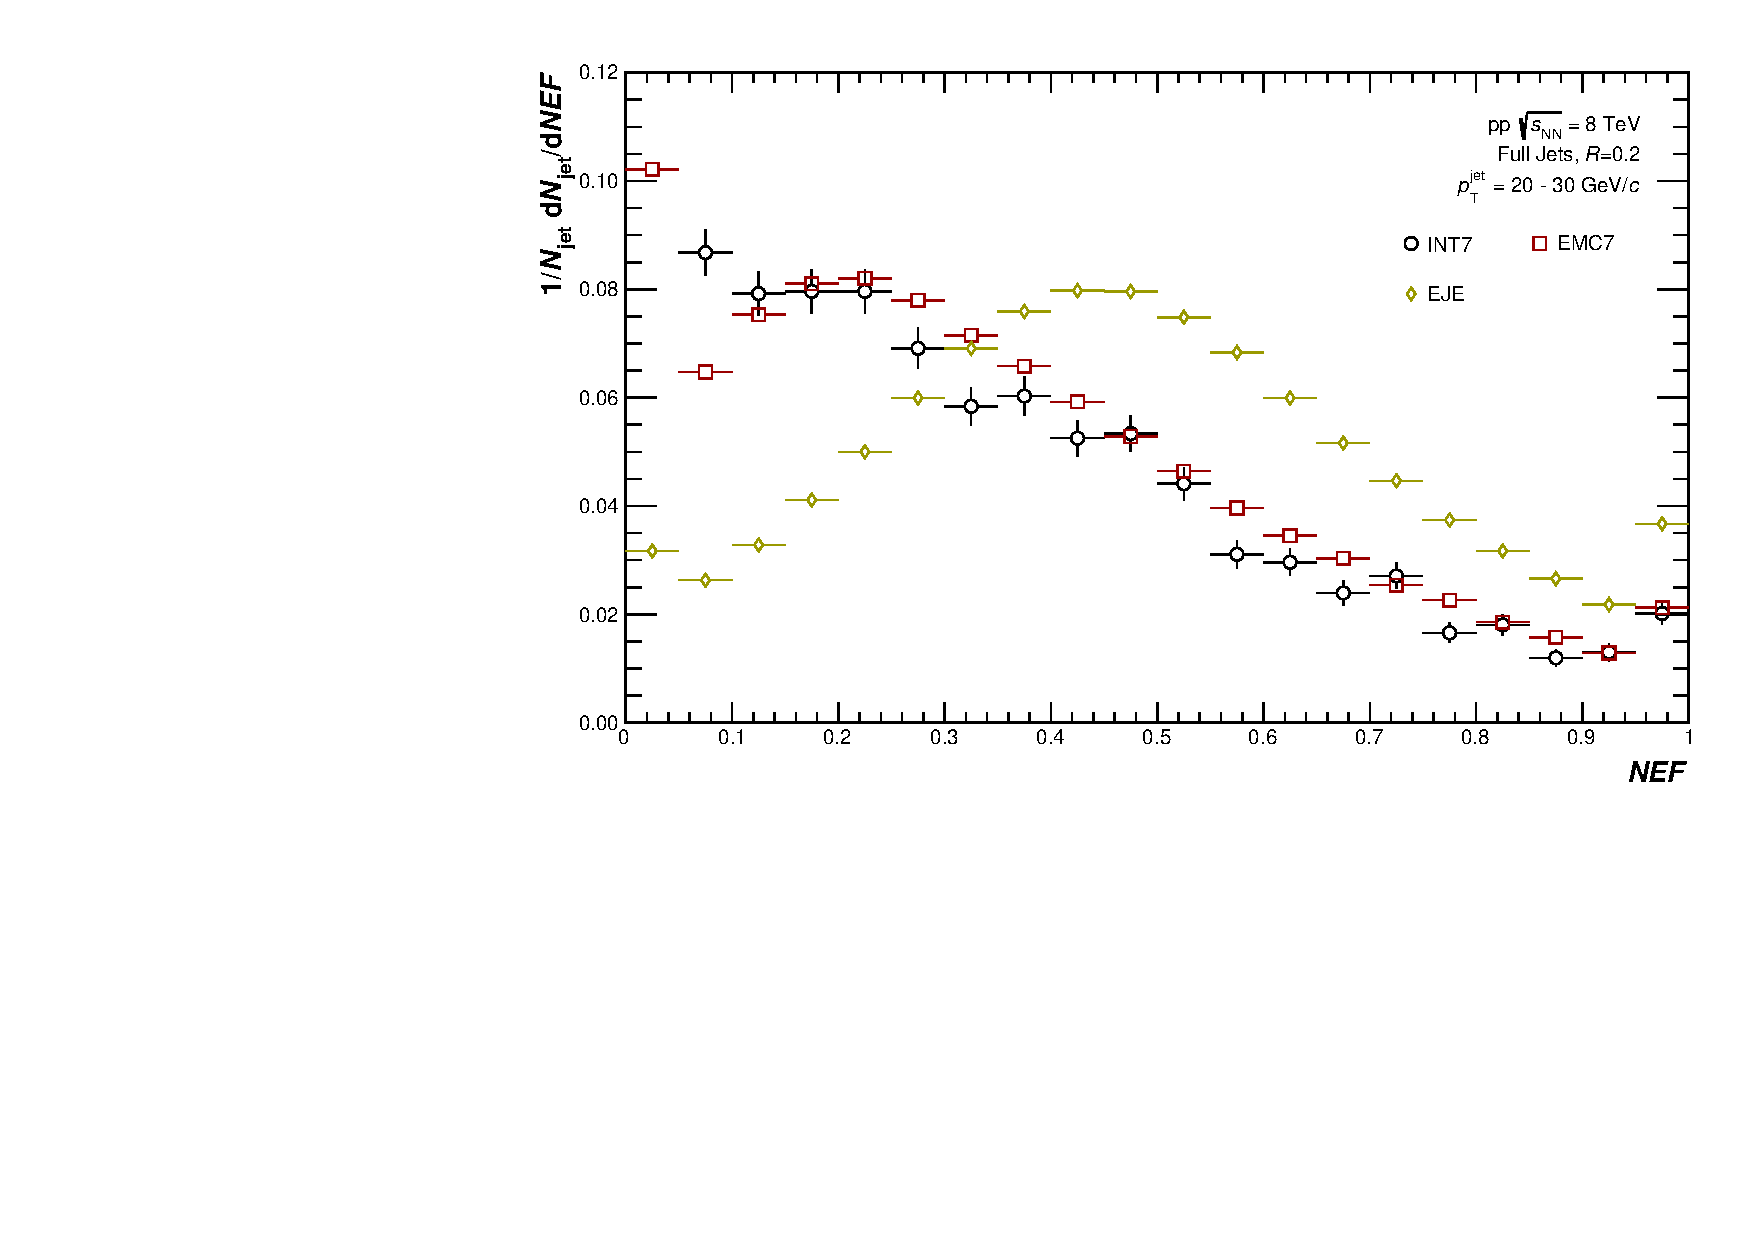
\includegraphics[width=7.5cm]{figures/NEF/All/hNEF_20-30GeV_R02.pdf}
            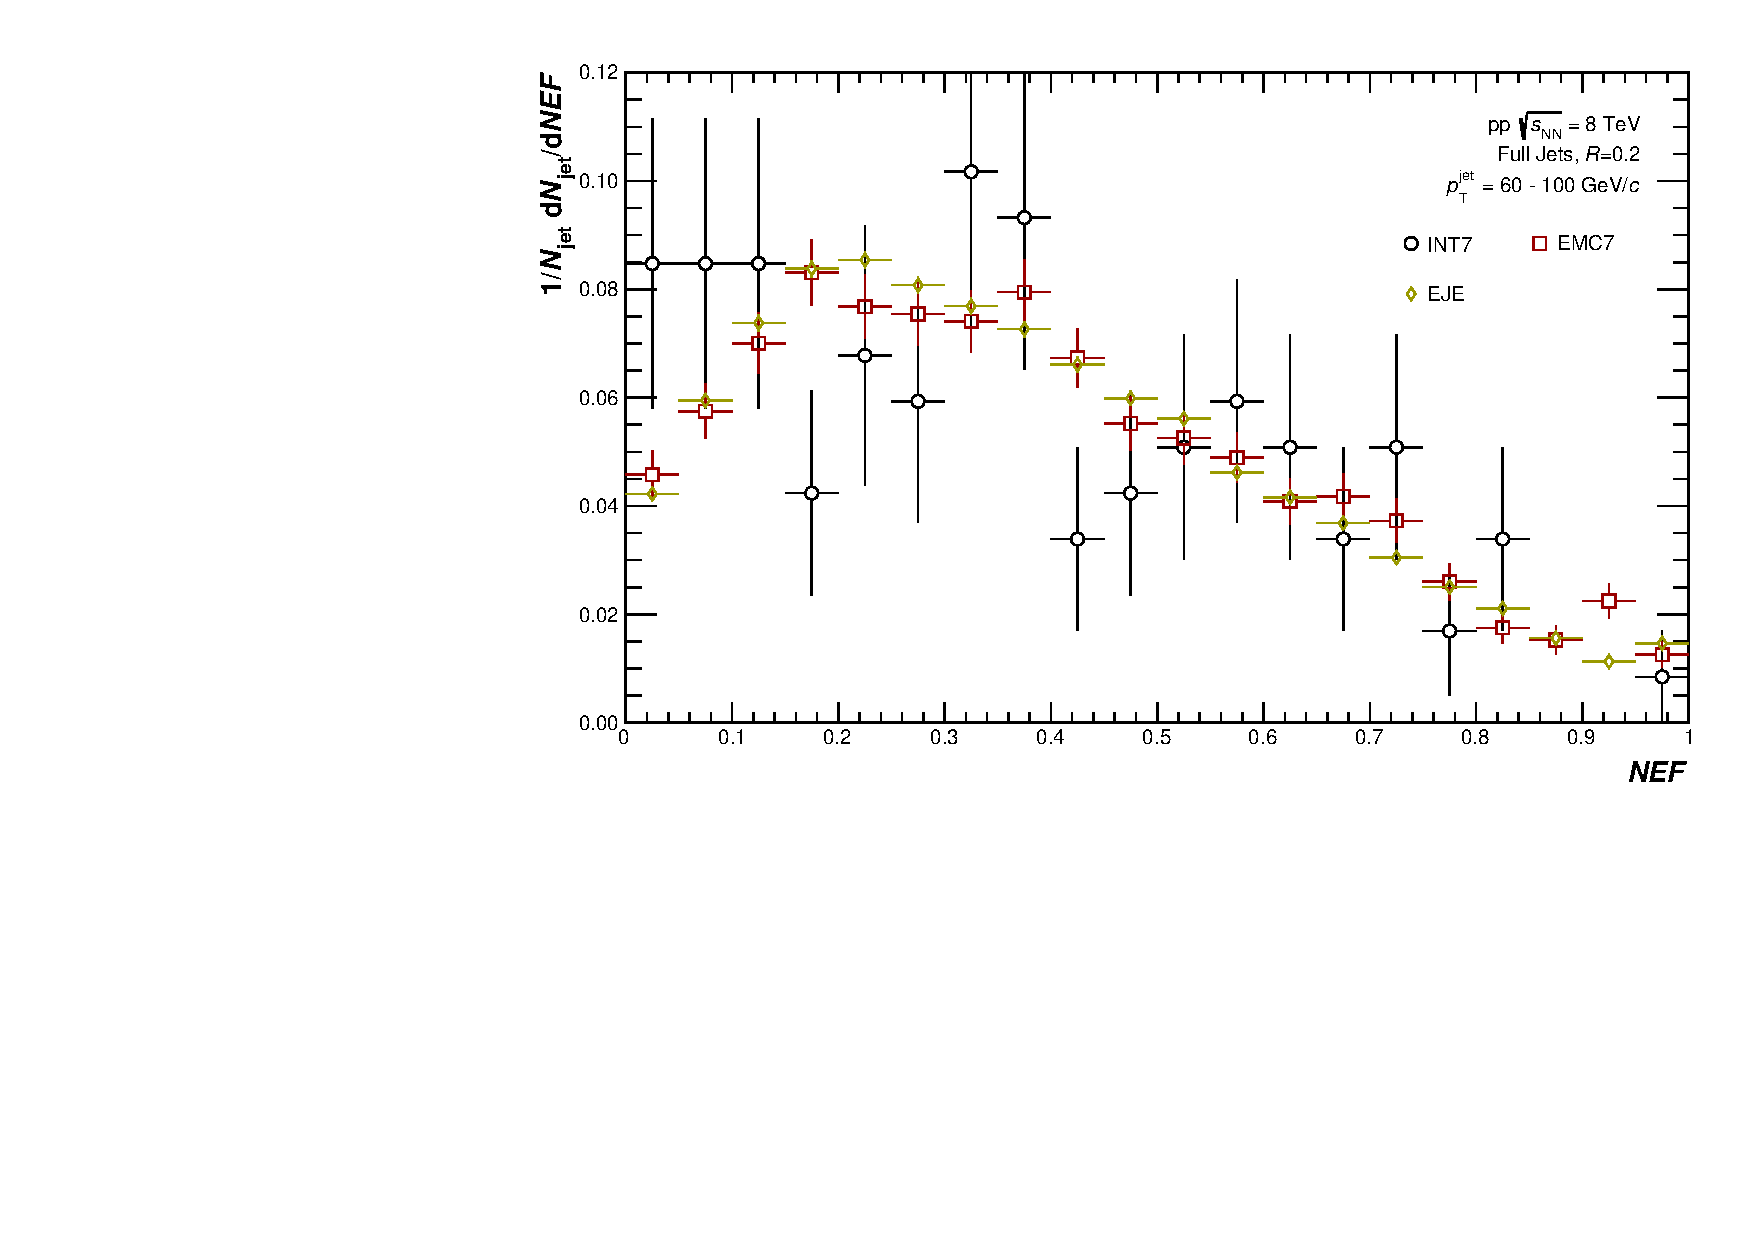
\includegraphics[width=7.5cm]{figures/NEF/All/hNEF_60-100GeV_R02.pdf}
            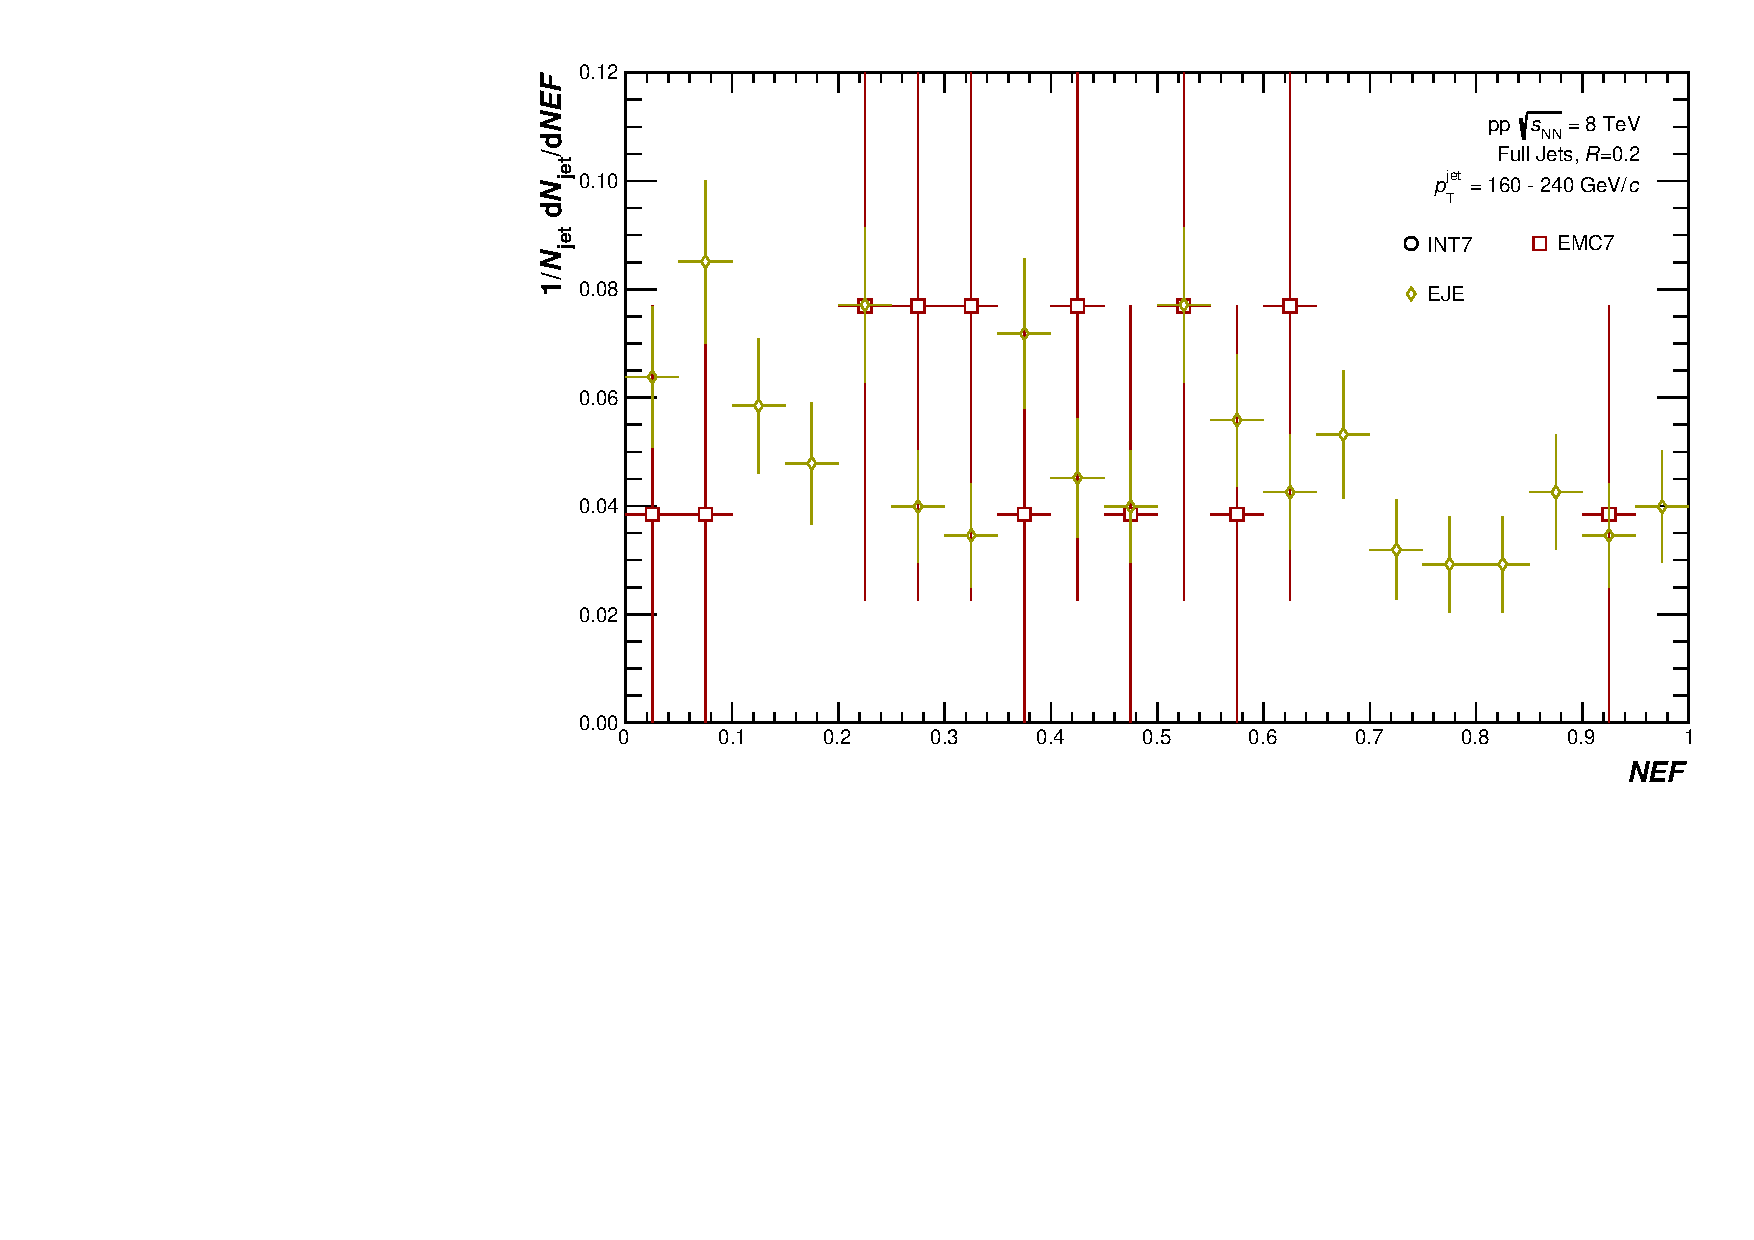
\includegraphics[width=7.5cm]{figures/NEF/All/hNEF_160-240GeV_R02.pdf}
        \vfill\null
        \columnbreak
            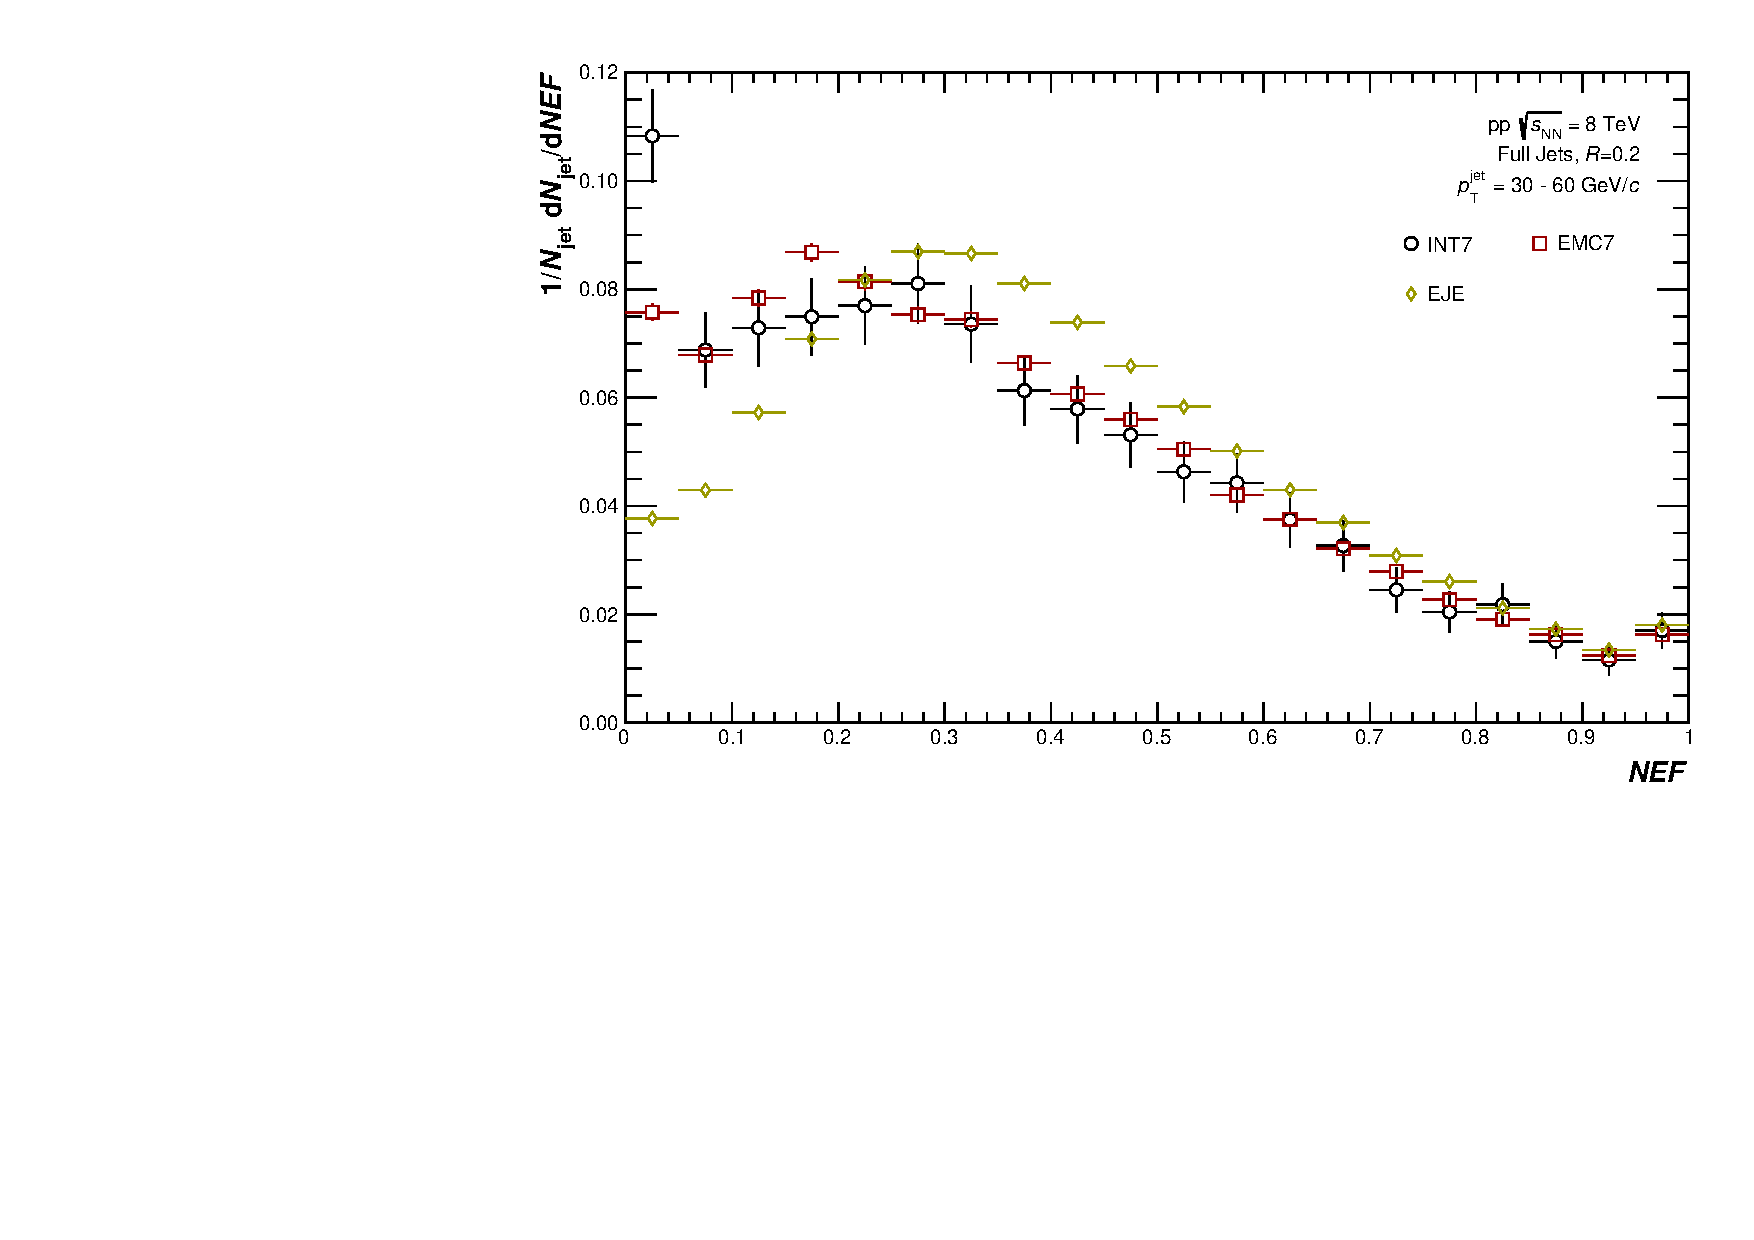
\includegraphics[width=7.5cm]{figures/NEF/All/hNEF_30-60GeV_R02.pdf}
            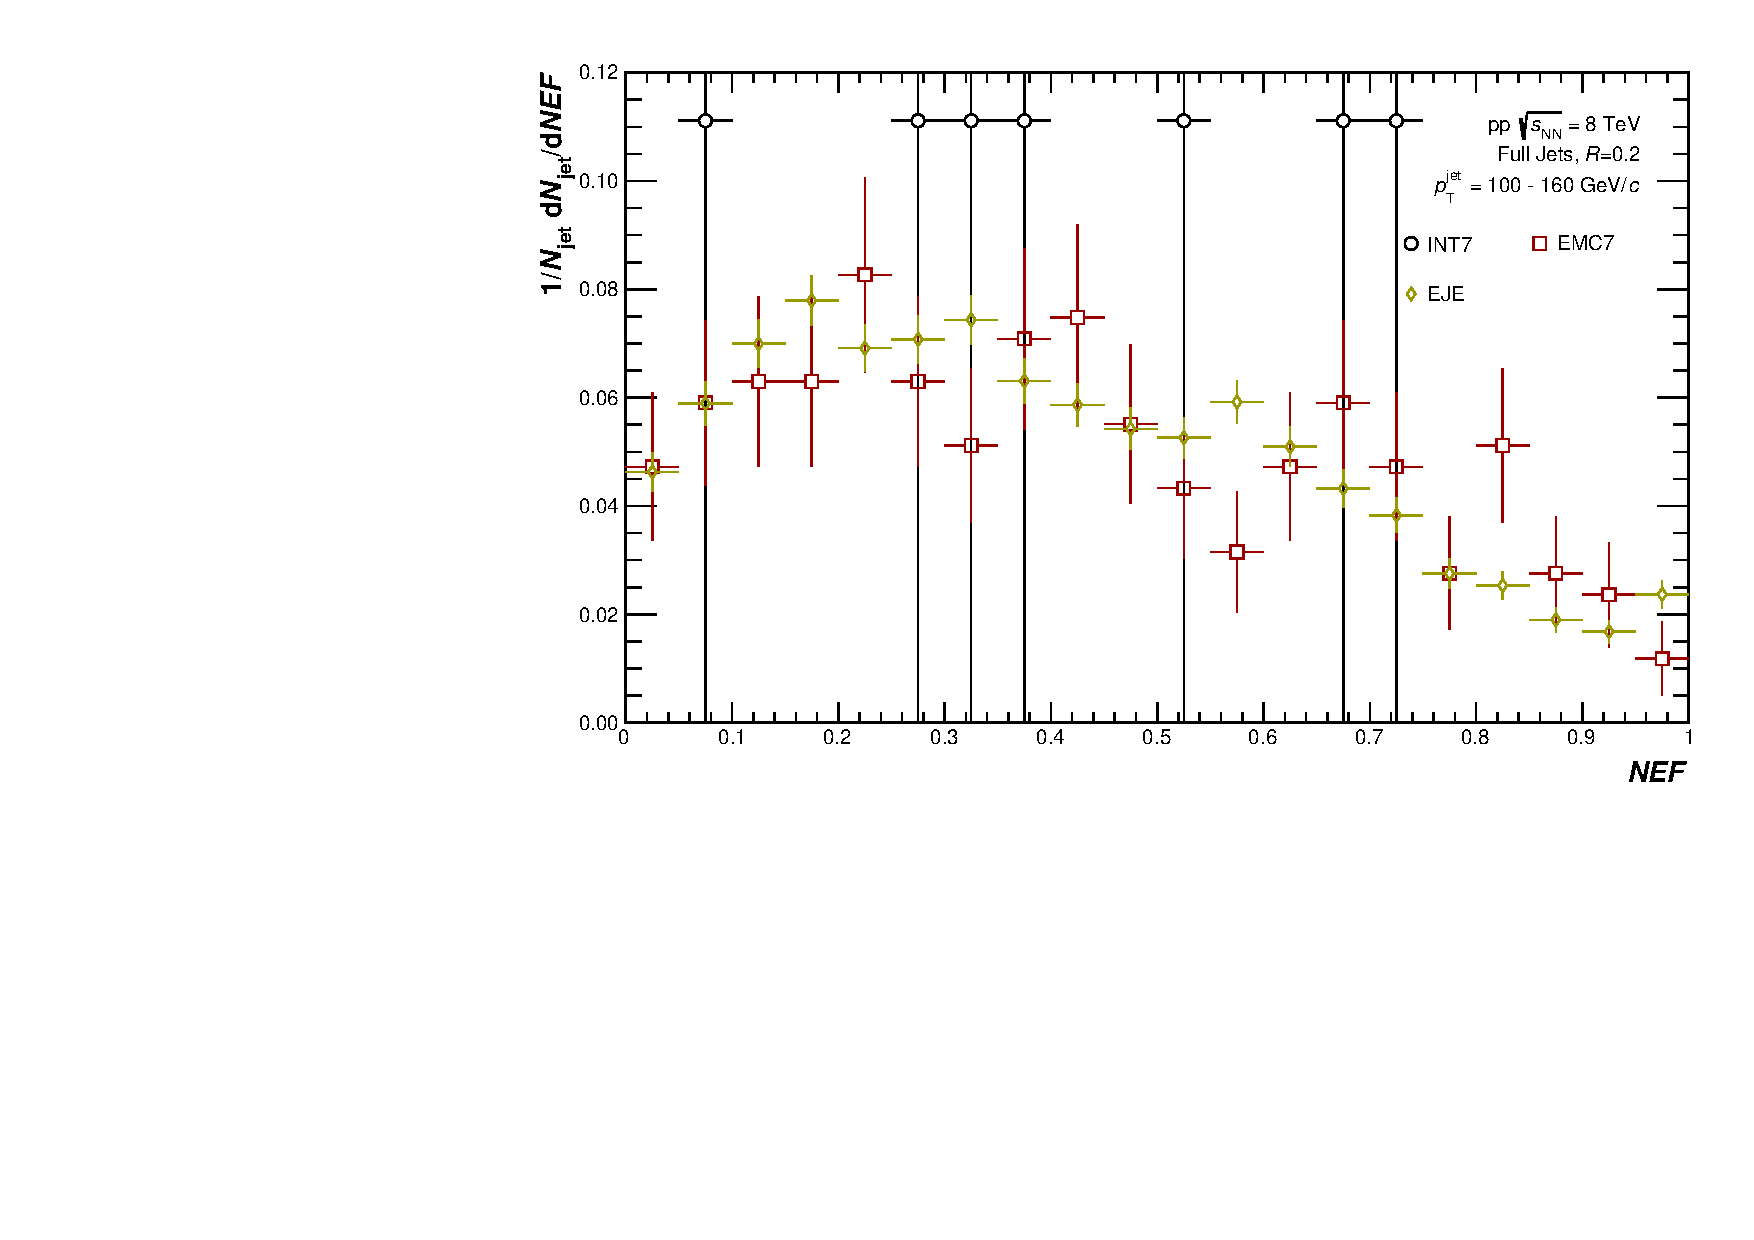
\includegraphics[width=7.5cm]{figures/NEF/All/hNEF_100-160GeV_R02.pdf}
        \vfill\null
    \end{multicols}
    \caption{Neutral energy fraction for jets \DIFaddbeginFL \DIFaddFL{in }\pp \DIFaddFL{collisions }\DIFaddendFL found using the minimum bias and EMCal triggers for different bins in jet energy using R = 0.2 jets.}
    \label{fig:NEF}
\end{figure}

\begin{figure}[h!]
    \centering
    \begin{multicols}{2}
            \includegraphics[width=7.5cm]{figures/TriggerSwap/ratio_EMCINT_data.pdf}
        \vfill\null 
        \columnbreak
            \includegraphics[width=7.5cm]{figures/TriggerSwap/ratio_EJEEMC_data.pdf}
        \vfill\null
    \end{multicols}
    \caption{Ratios in \DIFaddbeginFL \pp \DIFaddendFL data of EMC7/INT7 triggers (left) and EJE/EMC7 triggers (right).}
    \label{fig:trigger_ratios}
\end{figure}

As the trigger selects jets based on its neutral energy component, it introduces a bias on the selected jets that vanishes only at higher \pT. Fig. \ref{fig:NEF} shows the comparison of the distribution of the neutral energy fraction (NEF) of \DIFaddbegin \pp \DIFaddend jets in min. bias and triggered events for various bins in \pT for R = 0.2 jets. For other radii \DIFaddbegin \DIFadd{and equivalent plots in }\pPb\DIFaddend , see appendix \ref{sec:appendixTriggerBias} \DIFaddbegin \DIFadd{\textcolor{red}{remember to put the \pPb plots in the appendix}. }\DIFaddend The NEF is the fraction of the total energy of the track + EMCal cluster that comes from the neutral component. At lower \pT, the distribution in EMCal triggered events is shifted towards higher NEF values, since for jets close to the threshold, the dominant part of the energy must originate from neutral particles in order to fire the trigger. Only for jets with \pT larger than 30 (60) GeV/c, the distributions for the EMC7 (EJE) trigger start overlapping with the distribution in minimum bias events \DIFaddbegin \DIFadd{(for }\pPb\DIFadd{, this occurs at \textcolor{red}{? (?)} for the EJ2 (EJ1) trigger)}\DIFaddend . Additionally, at lower \pT, an effect can be seen from the different track and cluster \pT cutoffs (150 MeV for tracks, 300 MeV for clusters). As jet \pT decreases, it is more likely to find tracks than clusters, since the cutoff for tracks is lower. As jet \pT increases, the distributions begin to overlap. This is apparent in the 30-60 GeV/c region, but minimum bias statistics are too small to see beyond this \pT region. This effect can also be seen in figure 100 of the 2022 EMCal Performance paper \cite{EMCalPerformance}. Fig. \ref{fig:trigger_ratios} shows the \pT dependence of the jet yield ratio of trigger/min bias, which rises with \pT until a plateau is reached at 30 (60) GeV. At this point, the trigger is fully efficient, and the bias vanishes. For the analysis, jets are selected in triggered events only in the region where the trigger is bias-free. This will be discussed further in section \ref{sec:triggerCorrection}.

The trigger response in simulations is obtained by applying the same sliding window algorithm as implemented in the trigger hardware. A single EMCal FEE card provides readout for 32 towers, arranged in an 8x4 configuration. A FastOR covers a 2x2 tower group, and can cross boundaries between FEE cards. It provides a fast way to determine whether the 2x2 group is above a given threshold, as well as a rough energy reading. The trigger patches are calculated based on the energy from overlapping 4x4 tower sums that come from the FEE (Front End Electronics) simulation summed to FastORs. As the energy measurements in the trigger hardware suffer from residual decalibration, the energy is smeared based on the correlation between the energy measured in the FastOR and the calibrated FEE energy obtained from data. Realistic acceptance is simulated by removing FastOR energies based on the trigger mask in data. Triggered events are required to have at least one trigger patch above the nominal threshold. The description of the trigger bias in simulation is tested comparing the distributions of neutral energy fraction, z$_{ch}$, and z$_{neutral}$ between data and simulation. The objects z$_{ch}$ and z$_{neutral}$ are the fraction of the jet \pT coming from charged and neutral particles, respectively. Fig. \ref{fig:TriggerBiasNEFR02} shows the comparison of the neutral energy fraction for jets \DIFaddbegin \DIFadd{from }\pp \DIFadd{collisions }\DIFaddend with R=0.2 in triggered events between data and simulations for different bins in \pT (for other radii and the comparison of z$_{ch}$ and z$_{neutral}$ \DIFaddbegin \DIFadd{as well as the equivalent plots for }\pPb\DIFaddend , see appendix \ref{sec:appendixTriggerBiasRatios}) \DIFaddbegin \DIFadd{\textcolor{red}{remember to put the \pPb plots in the appendix}}\DIFaddend . The distributions obtained from simulation are in good agreement with the distributions obtained from data. 

Fig. \ref{fig:TriggerEfficiency} shows the trigger efficiency for jets with R=0.2 - R=0.6, obtained from taking the ratio of trigger/min. bias in simulations. The trigger gets adequately efficient at a jet \pT of 60 (30) GeV/c for the EJE (EMC7) trigger. In the low energy region, other detector effects which are not simulated (i.e. random noise) play a role. The simulated trigger efficiency will overpredict the correction, and thus the Monte-Carlo based correction can be trusted only in the higher-pt region of the turn-on.

\begin{figure}[h!]
    \centering
    \begin{multicols}{2}
            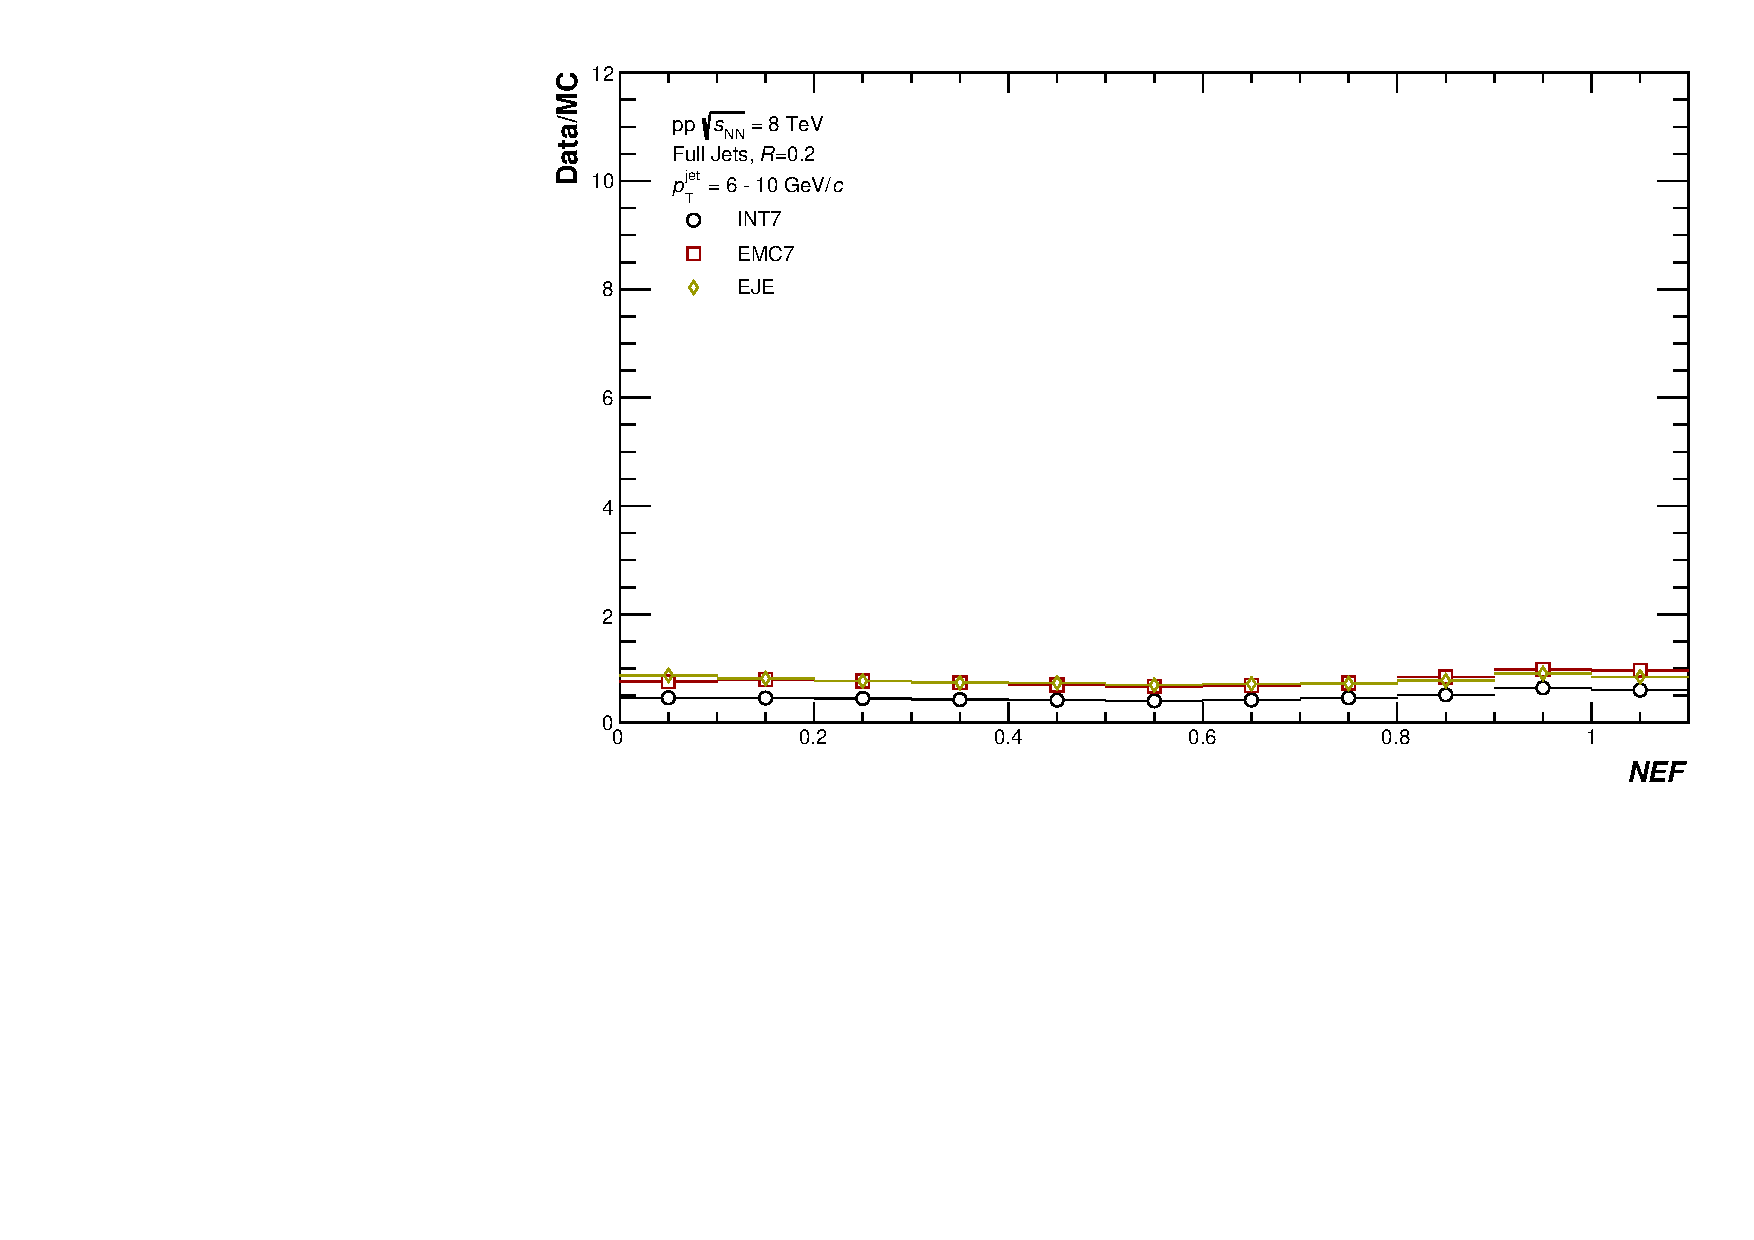
\includegraphics[width=7.5cm]{figures/TriggerBias/NEF/hNEF_ptBin0_R02.pdf}
            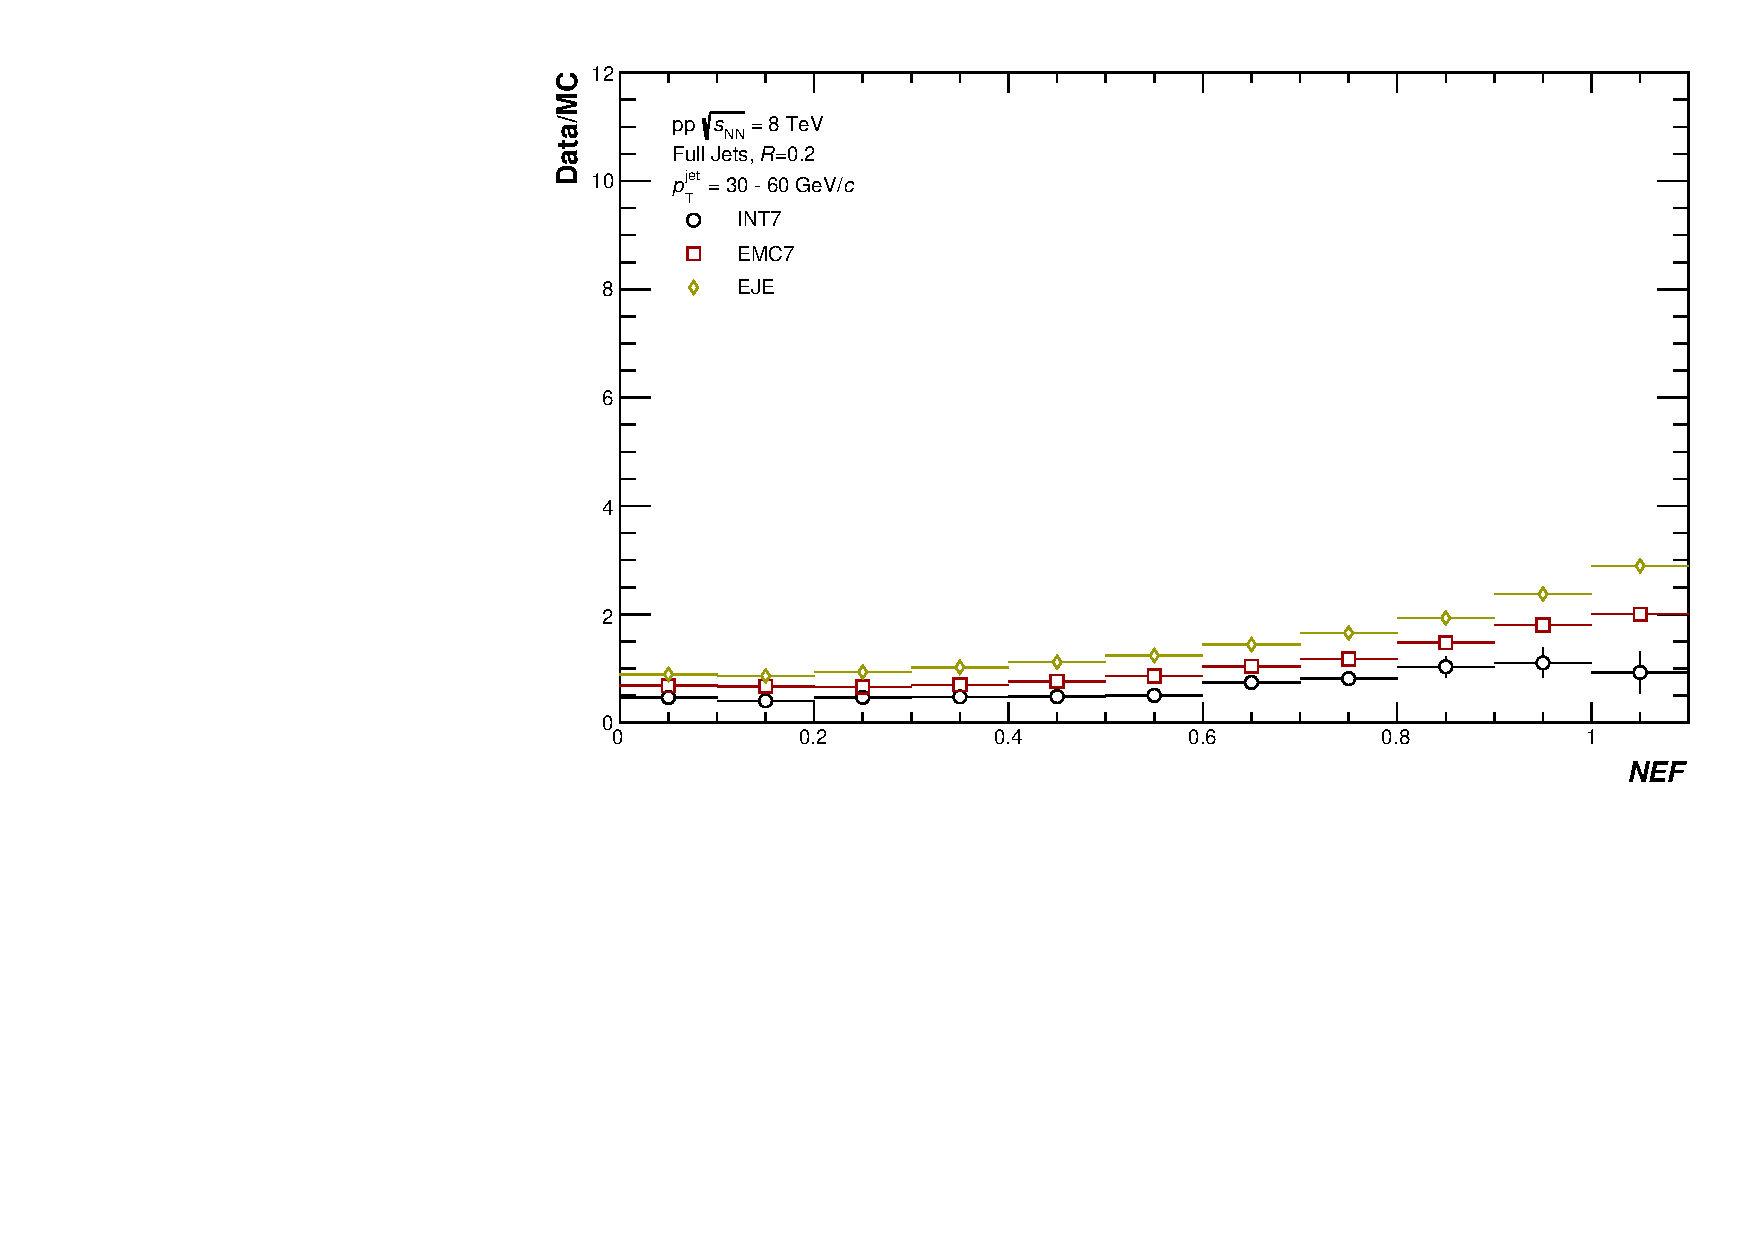
\includegraphics[width=7.5cm]{figures/TriggerBias/NEF/hNEF_ptBin2_R02.pdf}
            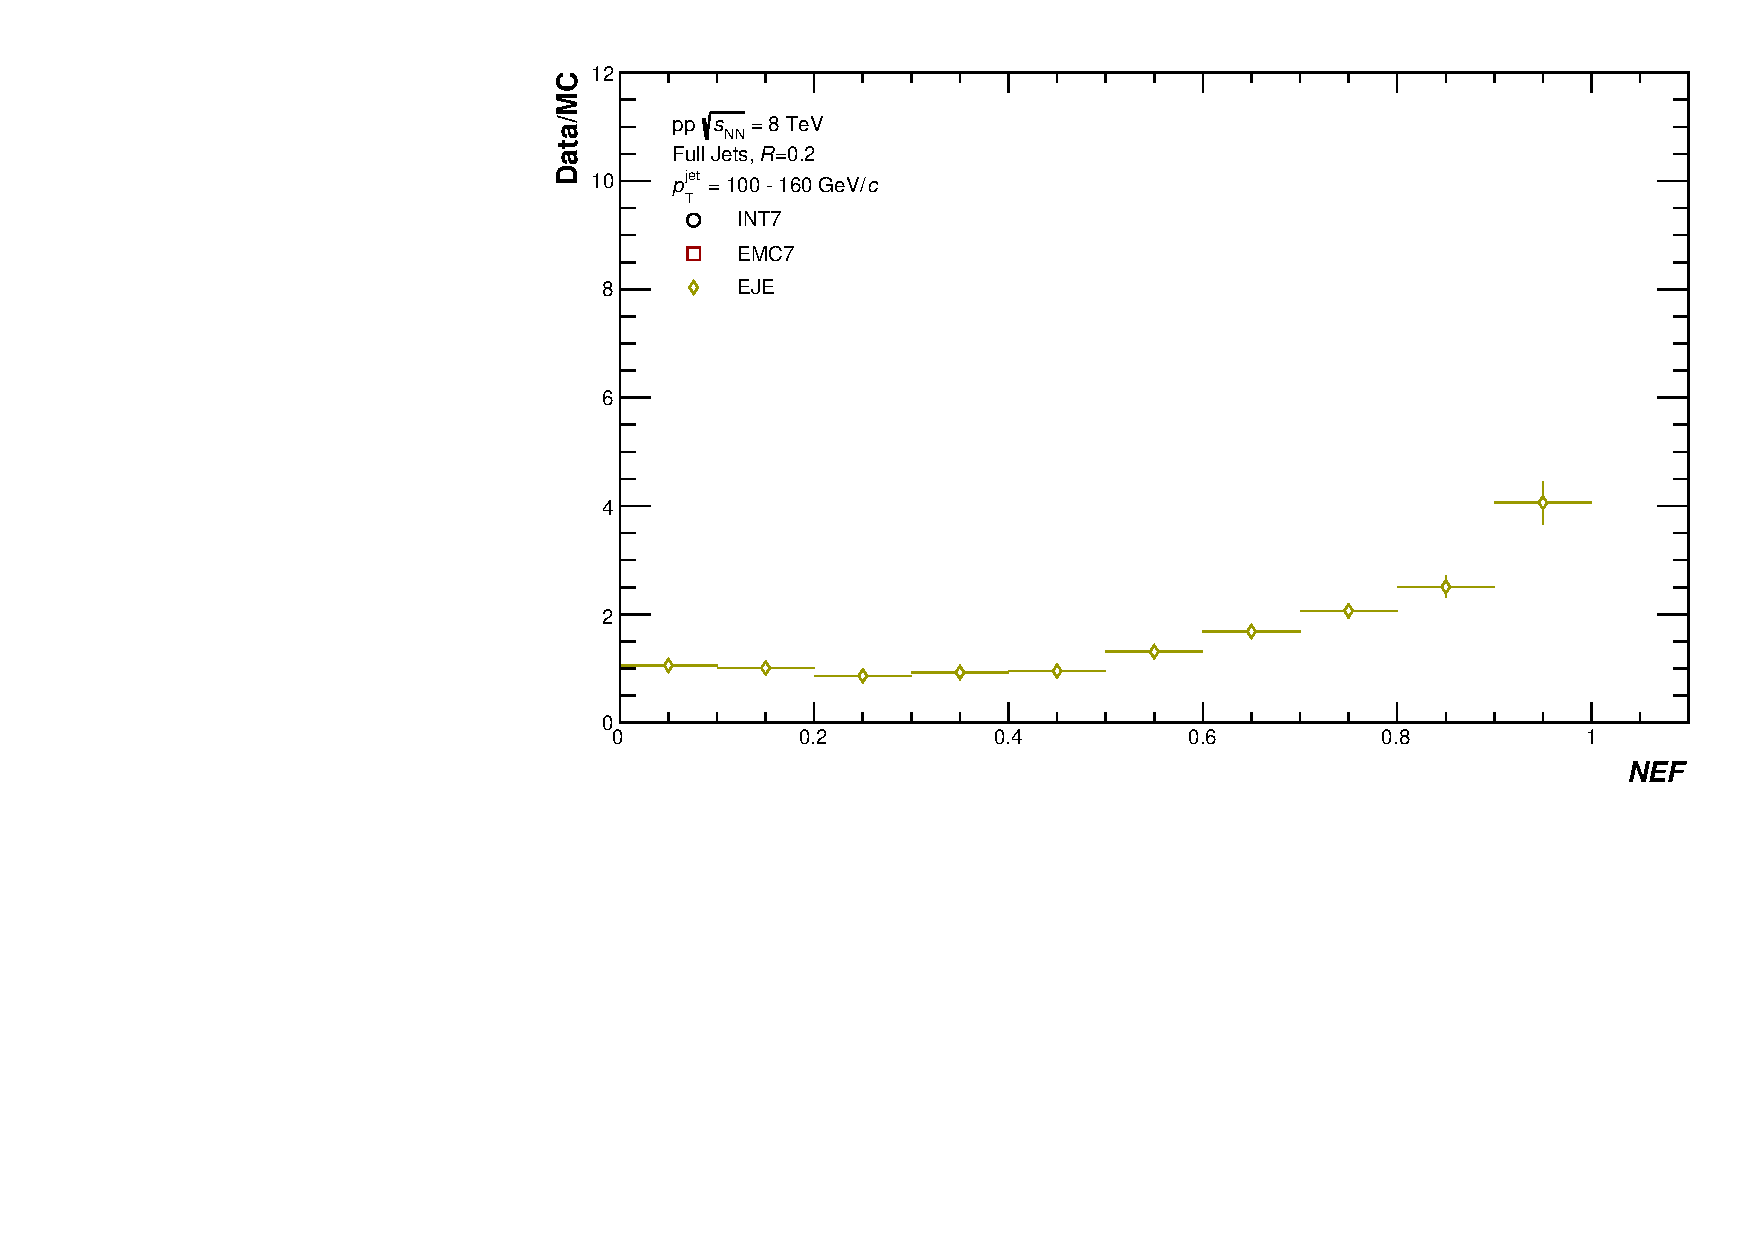
\includegraphics[width=7.5cm]{figures/TriggerBias/NEF/hNEF_ptBin4_R02.pdf}
        \vfill\null
        \columnbreak
            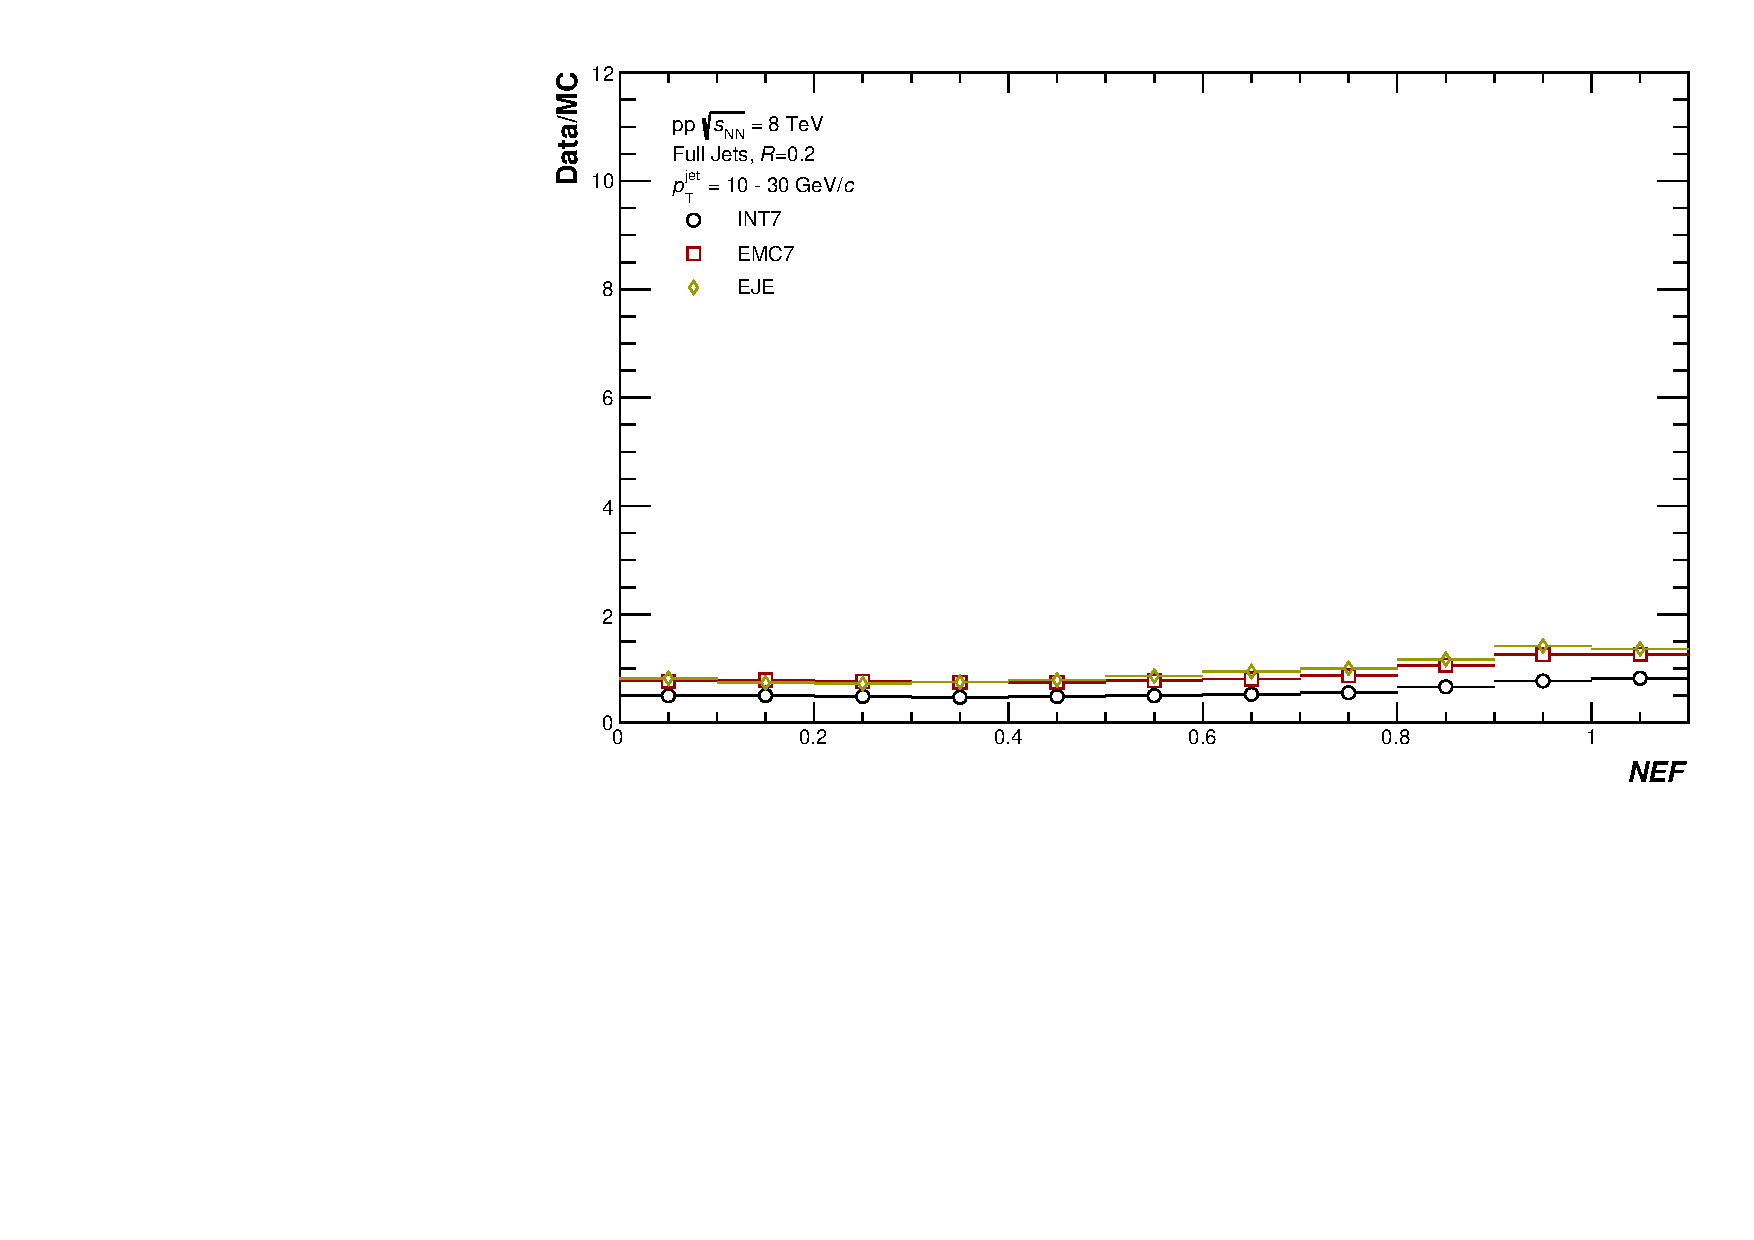
\includegraphics[width=7.5cm]{figures/TriggerBias/NEF/hNEF_ptBin1_R02.pdf}
            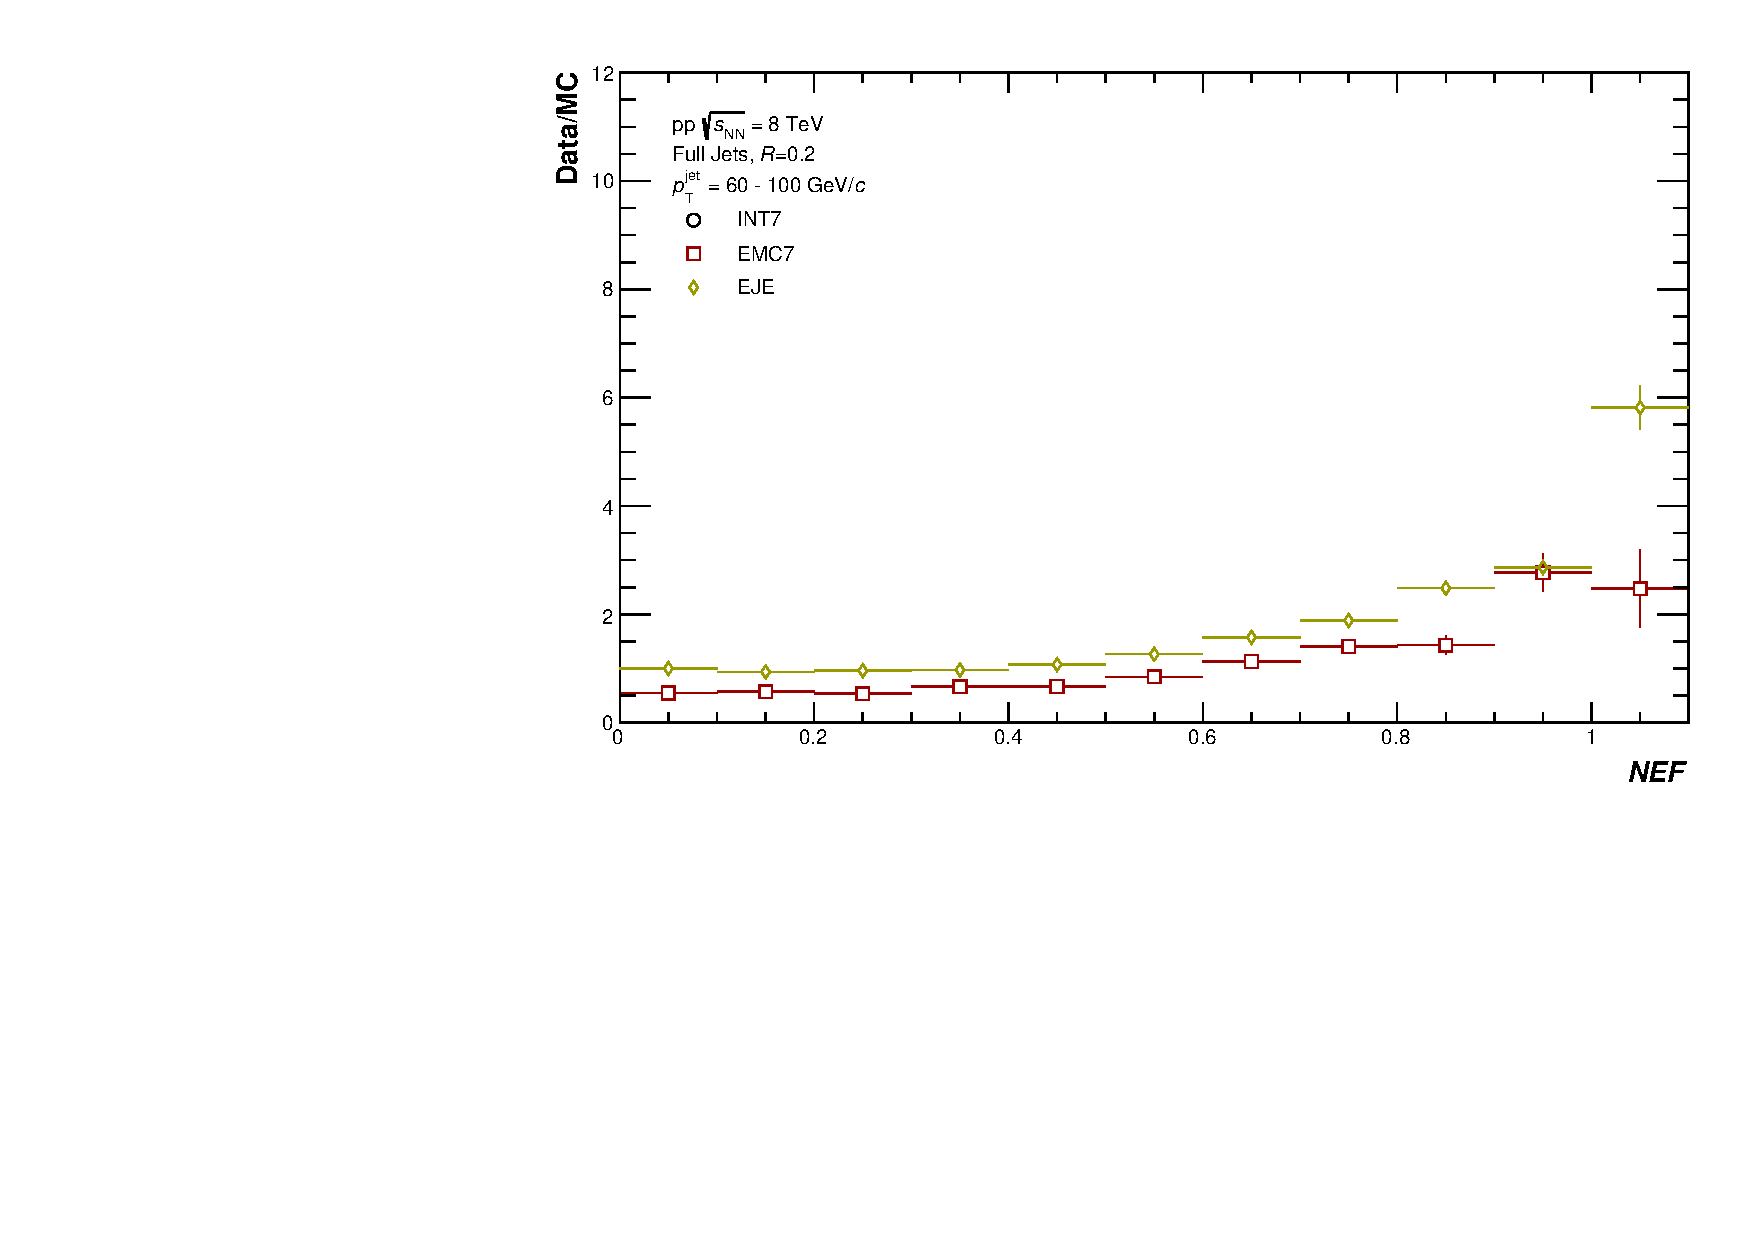
\includegraphics[width=7.5cm]{figures/TriggerBias/NEF/hNEF_ptBin3_R02.pdf}
            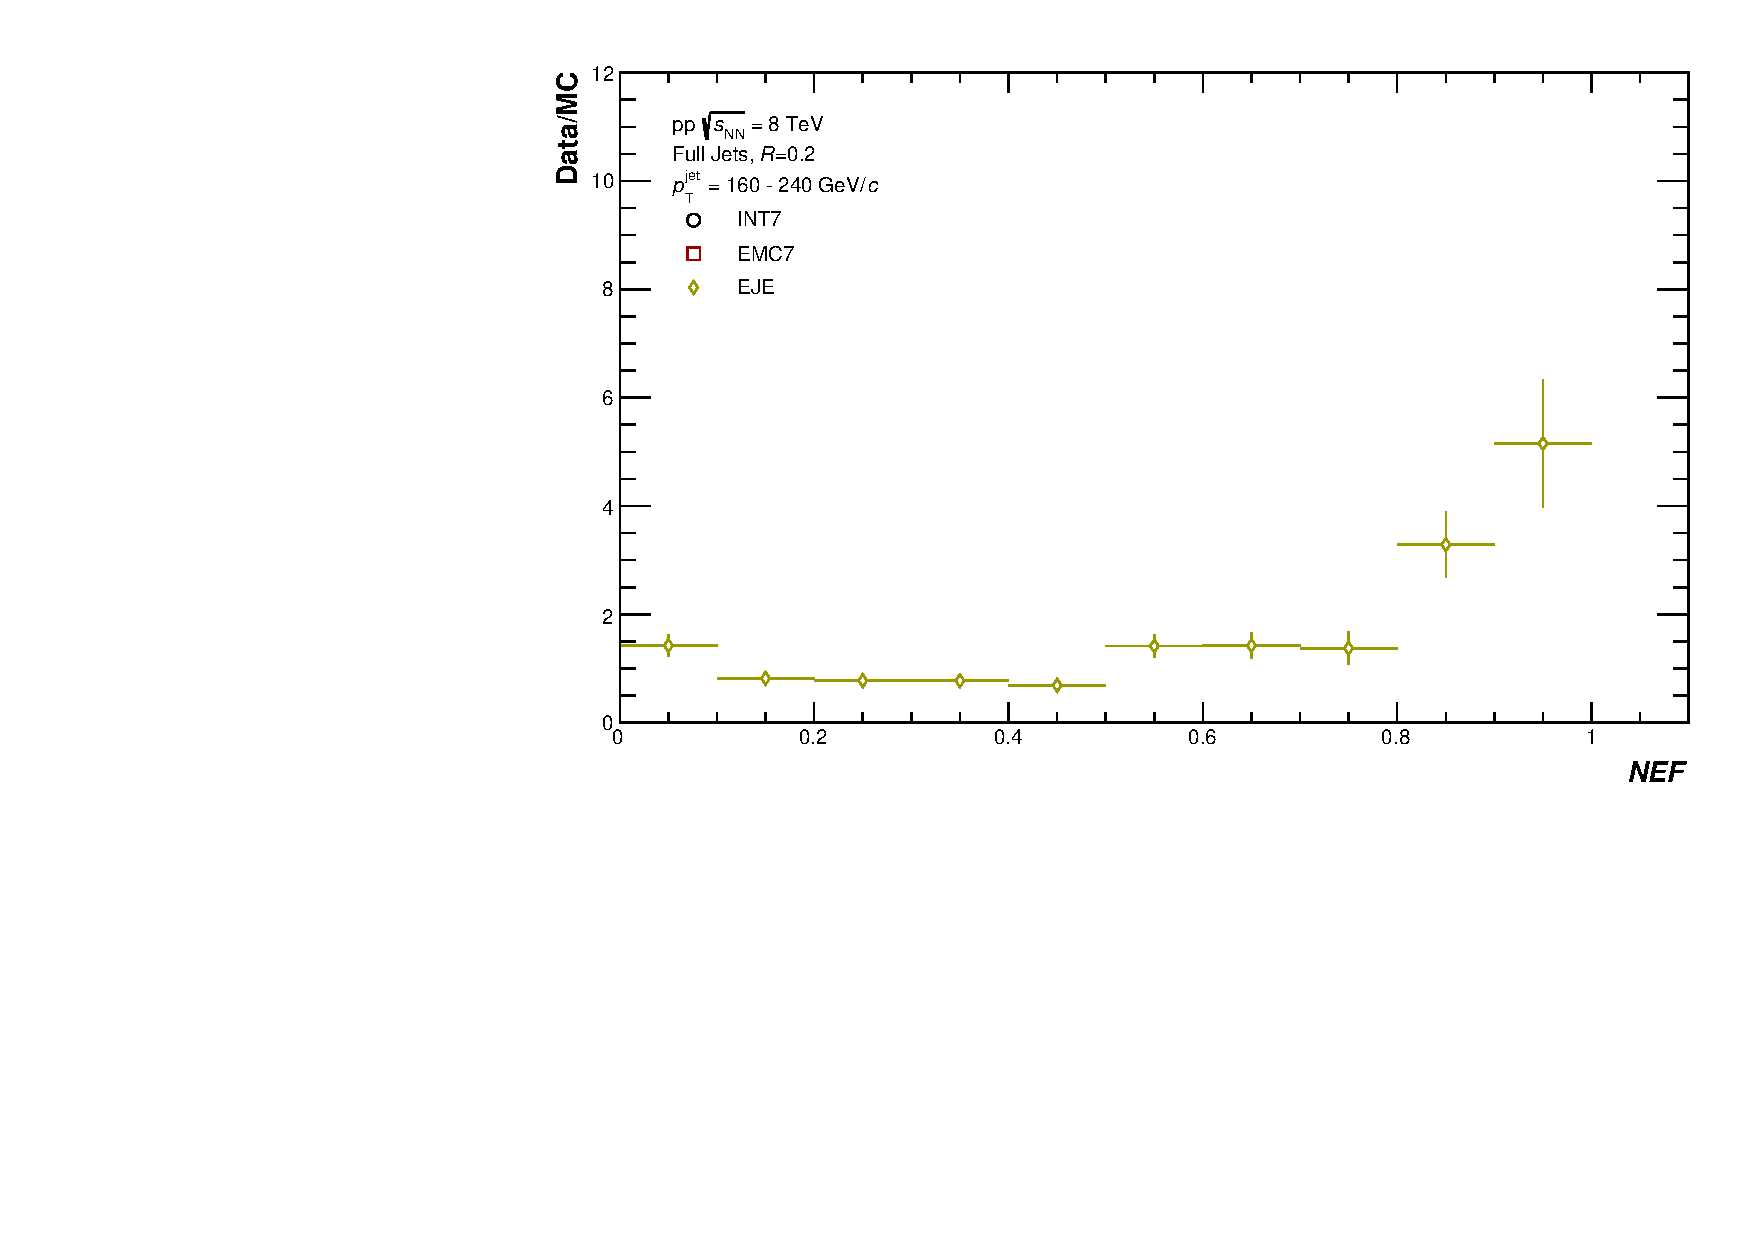
\includegraphics[width=7.5cm]{figures/TriggerBias/NEF/hNEF_ptBin5_R02.pdf}
        \vfill\null
    \end{multicols}
    \caption{NEF ratios of \DIFaddbeginFL \pp \DIFaddendFL data to MC for different bins in jet \DIFdelbeginFL \DIFdelFL{energy }\DIFdelendFL \DIFaddbeginFL \pT \DIFaddendFL and a jet radius of R=0.2.}
    \label{fig:TriggerBiasNEFR02}
\end{figure}

\begin{figure}[h!]
    \centering
    \begin{multicols}{2}
            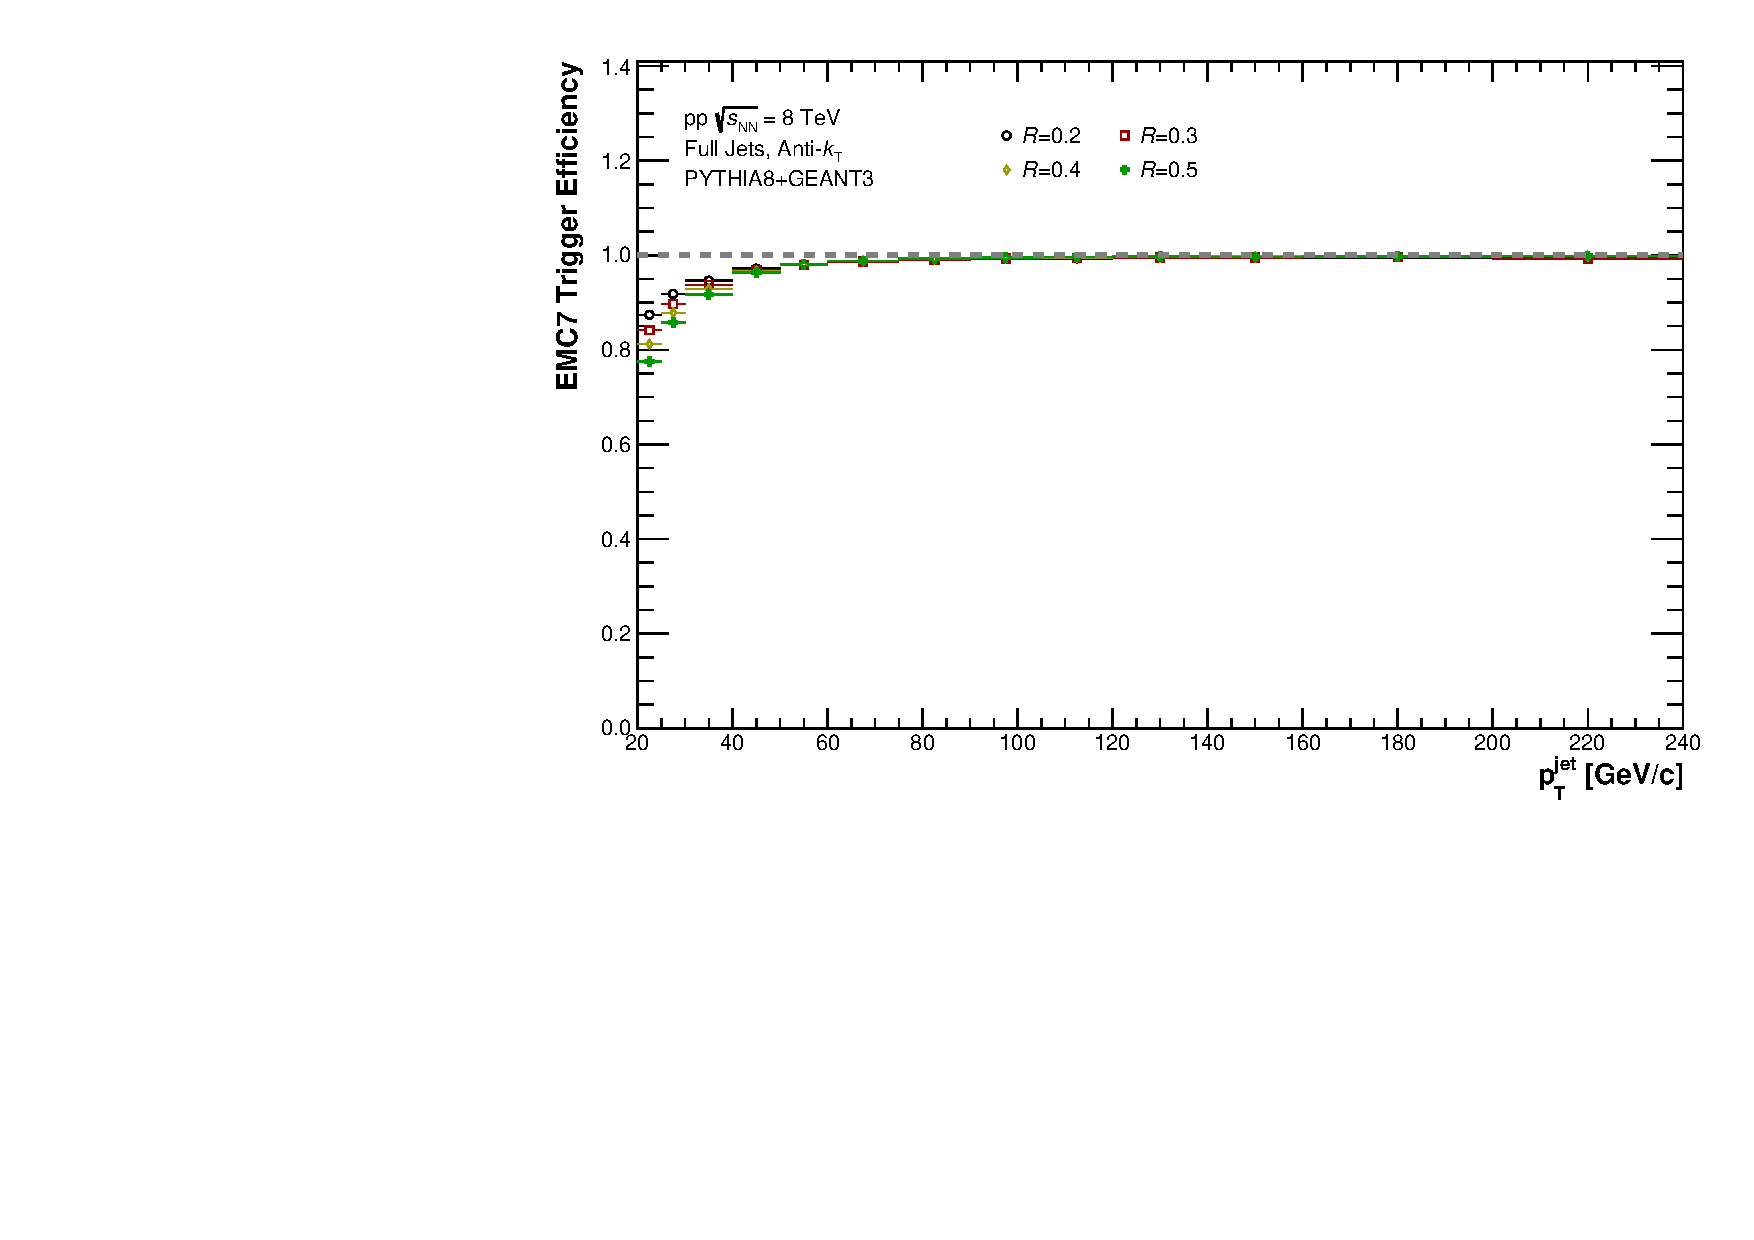
\includegraphics[width=7.5cm]{figures/TriggerEfficiency/hEfficiency_EMC7.pdf}
        \vfill\null
        \columnbreak
            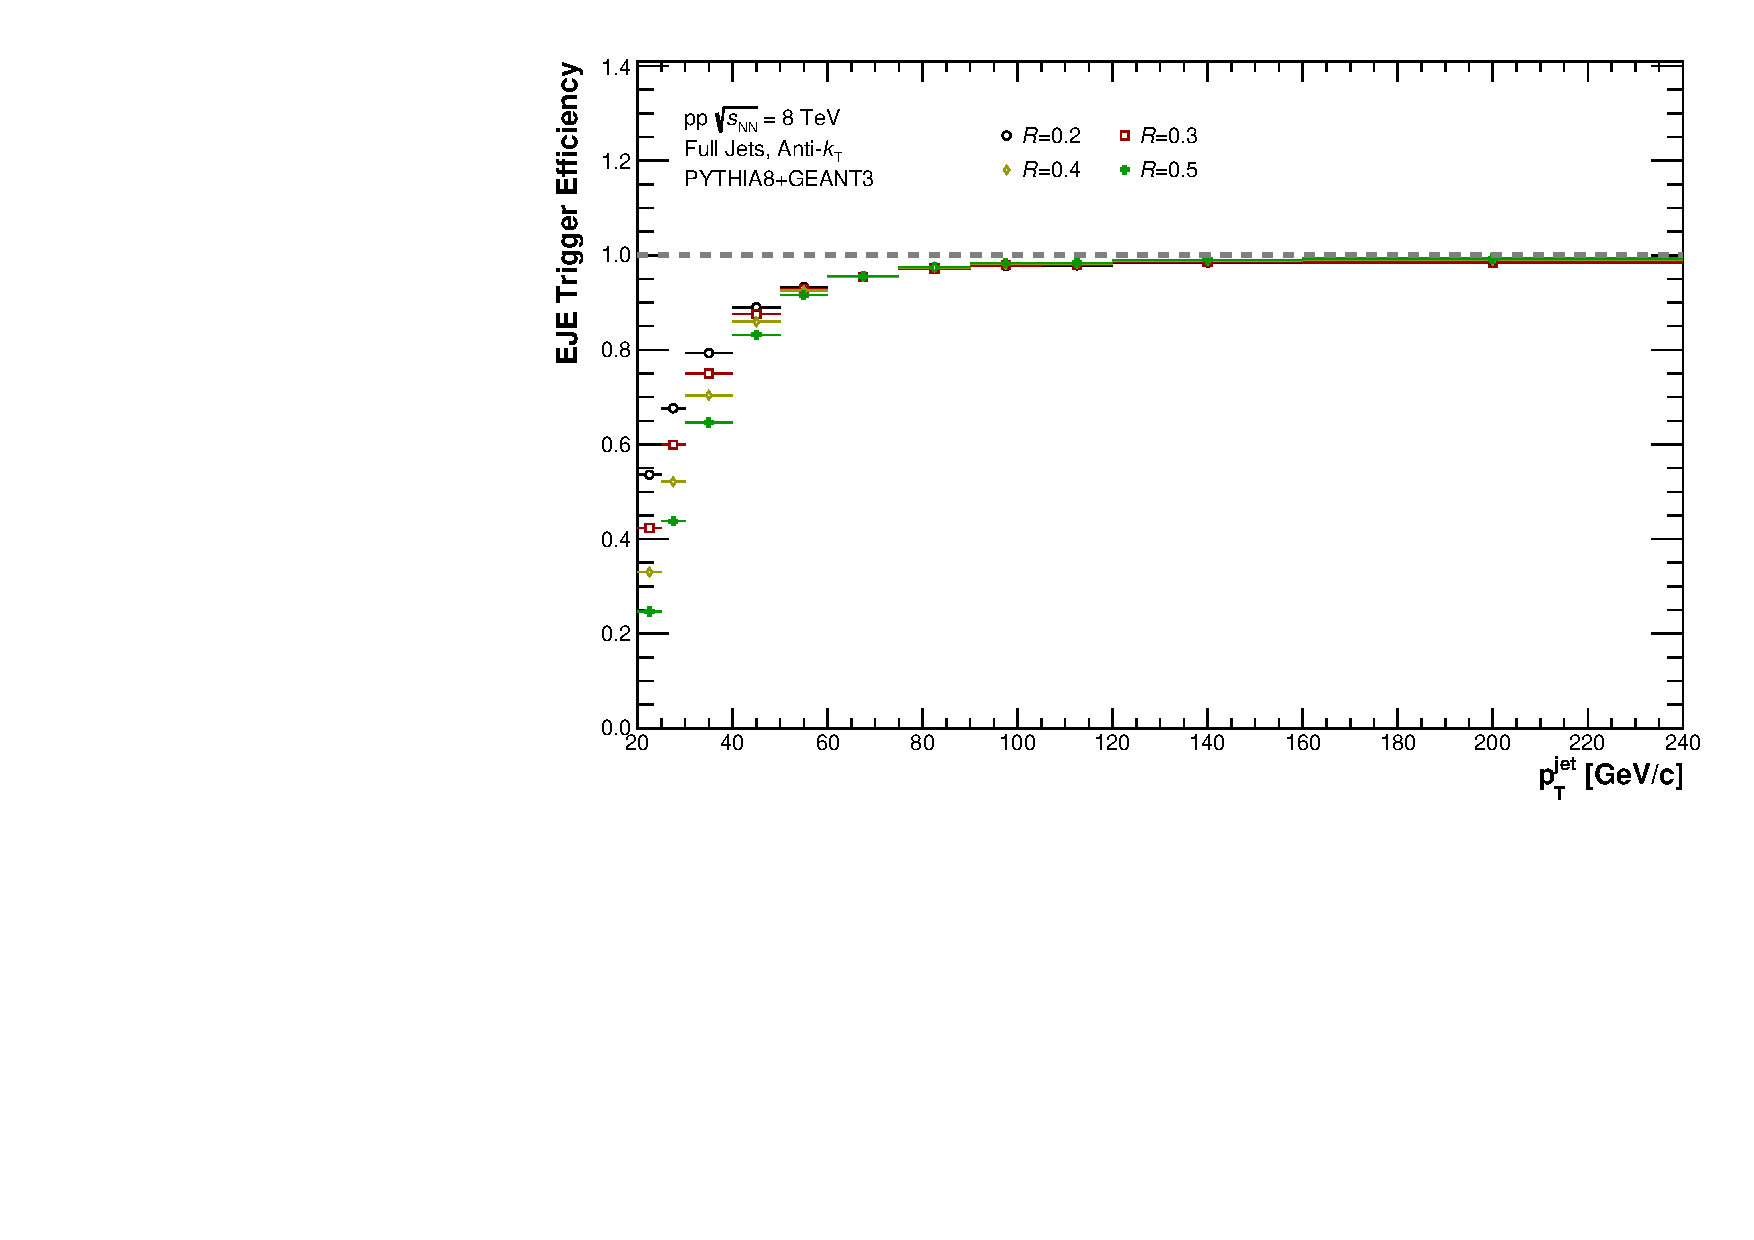
\includegraphics[width=7.5cm]{figures/TriggerEfficiency/hEfficiency_EJE.pdf}
        \vfill\null
    \end{multicols}
    \caption{Trigger efficiency for the EMC7 trigger (left) and the EJE trigger (right), found by taking the ratio of trigger/min bias in \DIFaddbeginFL \pp \DIFaddendFL simulation.}
    \label{fig:TriggerEfficiency}
\end{figure}

\subsection{Instrumental Response}
\label{sec:InstResponse}

\begin{figure}[h!]
    \centering
    \begin{multicols}{2}
            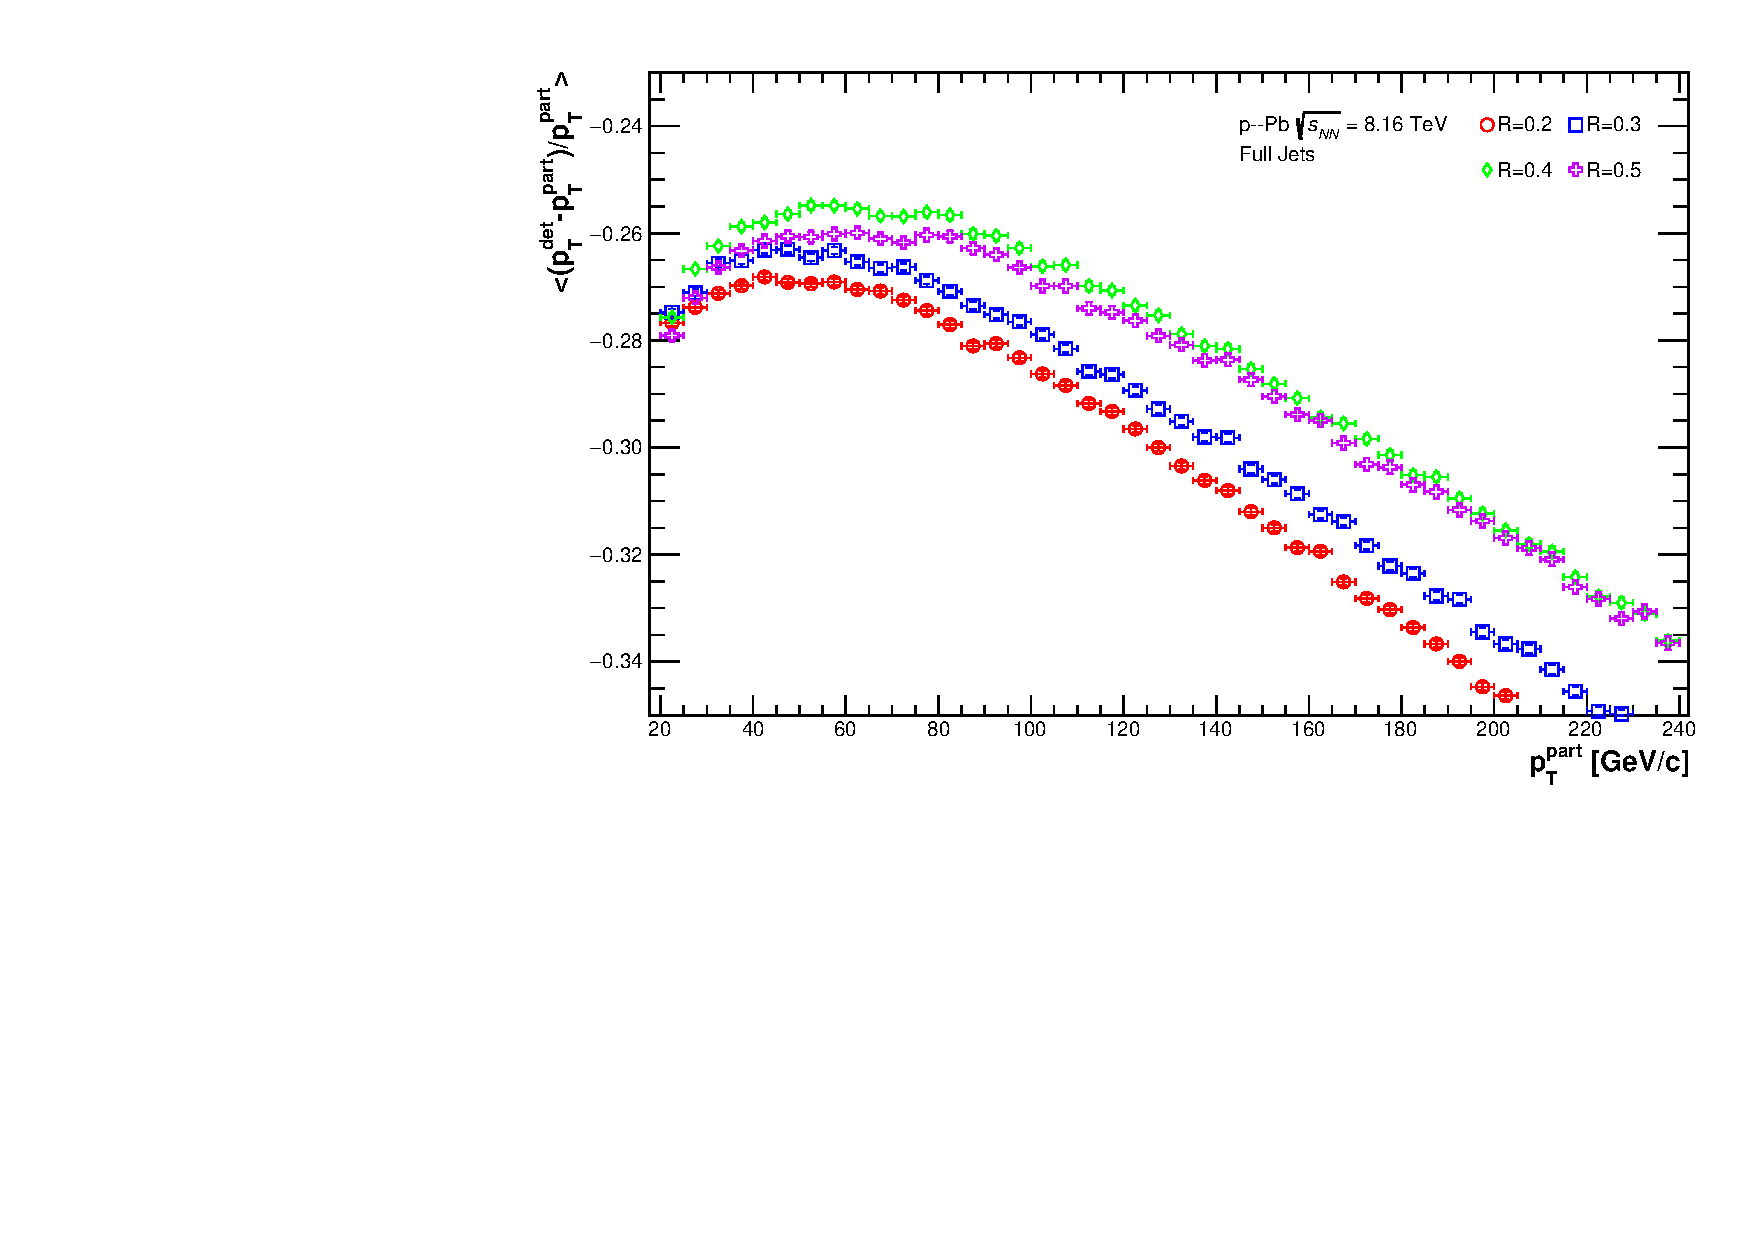
\includegraphics[width=7.5cm]{figures/EnergyScale/EnergyScaleMean.pdf}
        \vfill\null 
        \columnbreak
            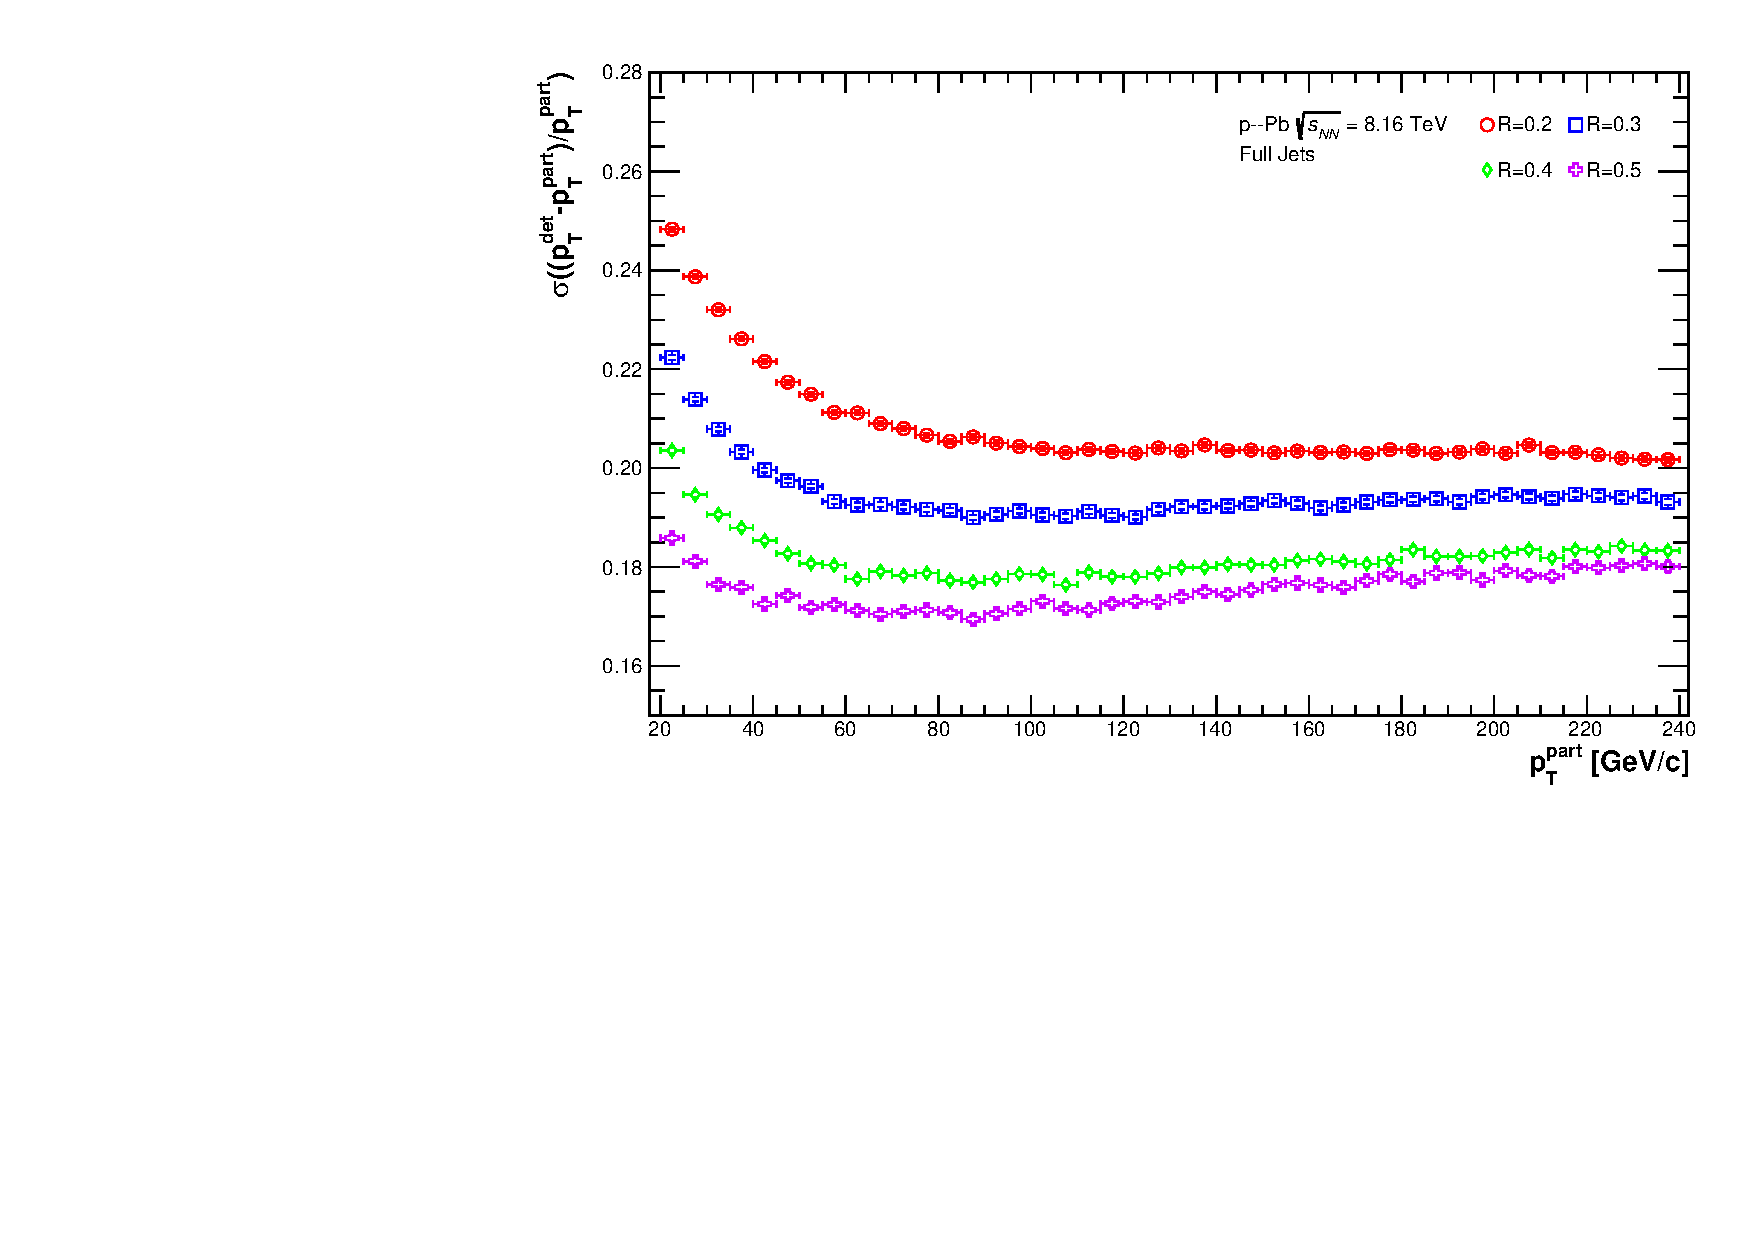
\includegraphics[width=7.5cm]{figures/EnergyScale/EnergyScaleWidth.pdf}
        \vfill\null
    \end{multicols}
    \caption{Jet energy scale (left) and jet energy resolution (right) showing the instrumental response \DIFaddbeginFL \DIFaddFL{for jets in }\pp \DIFaddFL{collisions}\DIFaddendFL .}
    \label{fig:EnergyScale}
\end{figure}

In order to quantify the detector effects on the observables\DIFdelbegin \DIFdel{in pp collisions, the }\DIFdelend \DIFaddbegin \DIFadd{, the PYTHIA }\DIFaddend production LHC16c2 was used \DIFdelbegin \DIFdel{. Events generated by PYTHIA }\DIFdelend \DIFaddbegin \DIFadd{for }\pp\DIFadd{, and the PYTHIA productions LHC23d7a and LHC23d7b were used for }\pPb\DIFadd{. LHC23d7a,b were further embedded in }\pPb \DIFadd{data in order to simulate a realistic background. This is further discussed in section \textcolor{red}{insert reference to embedding section}. Generated events }\DIFaddend were fully propagated using GEANT3 to form a detector response in \pT$^{jet}$, which is used to unfold the measured \DIFdelbegin \DIFdel{pp distributions in 2D }\DIFdelend \DIFaddbegin \DIFadd{jet distributions }\DIFaddend (see section \ref{sec:unfolding}). The instrumental response \DIFaddbegin \DIFadd{for }\pp \DIFadd{collisions }\DIFaddend is characterized in Fig. \ref{fig:EnergyScale}\DIFaddbegin \DIFadd{, while that for }\pPb \DIFadd{collisions can be found in Fig. \textcolor{red}{insert \pPb energy scale plots}}\DIFaddend . The left plot shows the jet energy scale shift, quantified as the mean of the residuals distribution, as function of the true jet \pT. We see a mild R dependence and a relative negative shift of around 27\% at \pT$^{jet}$ = 100 GeV/c due to finite tracking efficiency. The right plot shows the jet energy resolution, quantified as the RMS of the residuals distribution. We observe that the jet energy resolution is relatively flat for full jets at higher \pT due to the neutral constituents.

\DIFdelbegin \DIFdel{A }\DIFdelend \DIFaddbegin \DIFadd{For }\pp\DIFadd{, a }\DIFaddend comparison to the energy scale results from 13 TeV is also included, and can be seen in figure \ref{fig:EnergyScaleComp}. The larger the jet radius, the larger the difference gets compared to 13 TeV. This is likely due to detector performance effects. The performance for run 2 is significantly different, in part from a better resolution due to the inclusion of TRD tracking in ~50\% of events. Additionally, there was a smaller fraction of bad channels in the EMCal for run 2.

\begin{figure}[h!]
    \centering
    \begin{multicols}{2}
            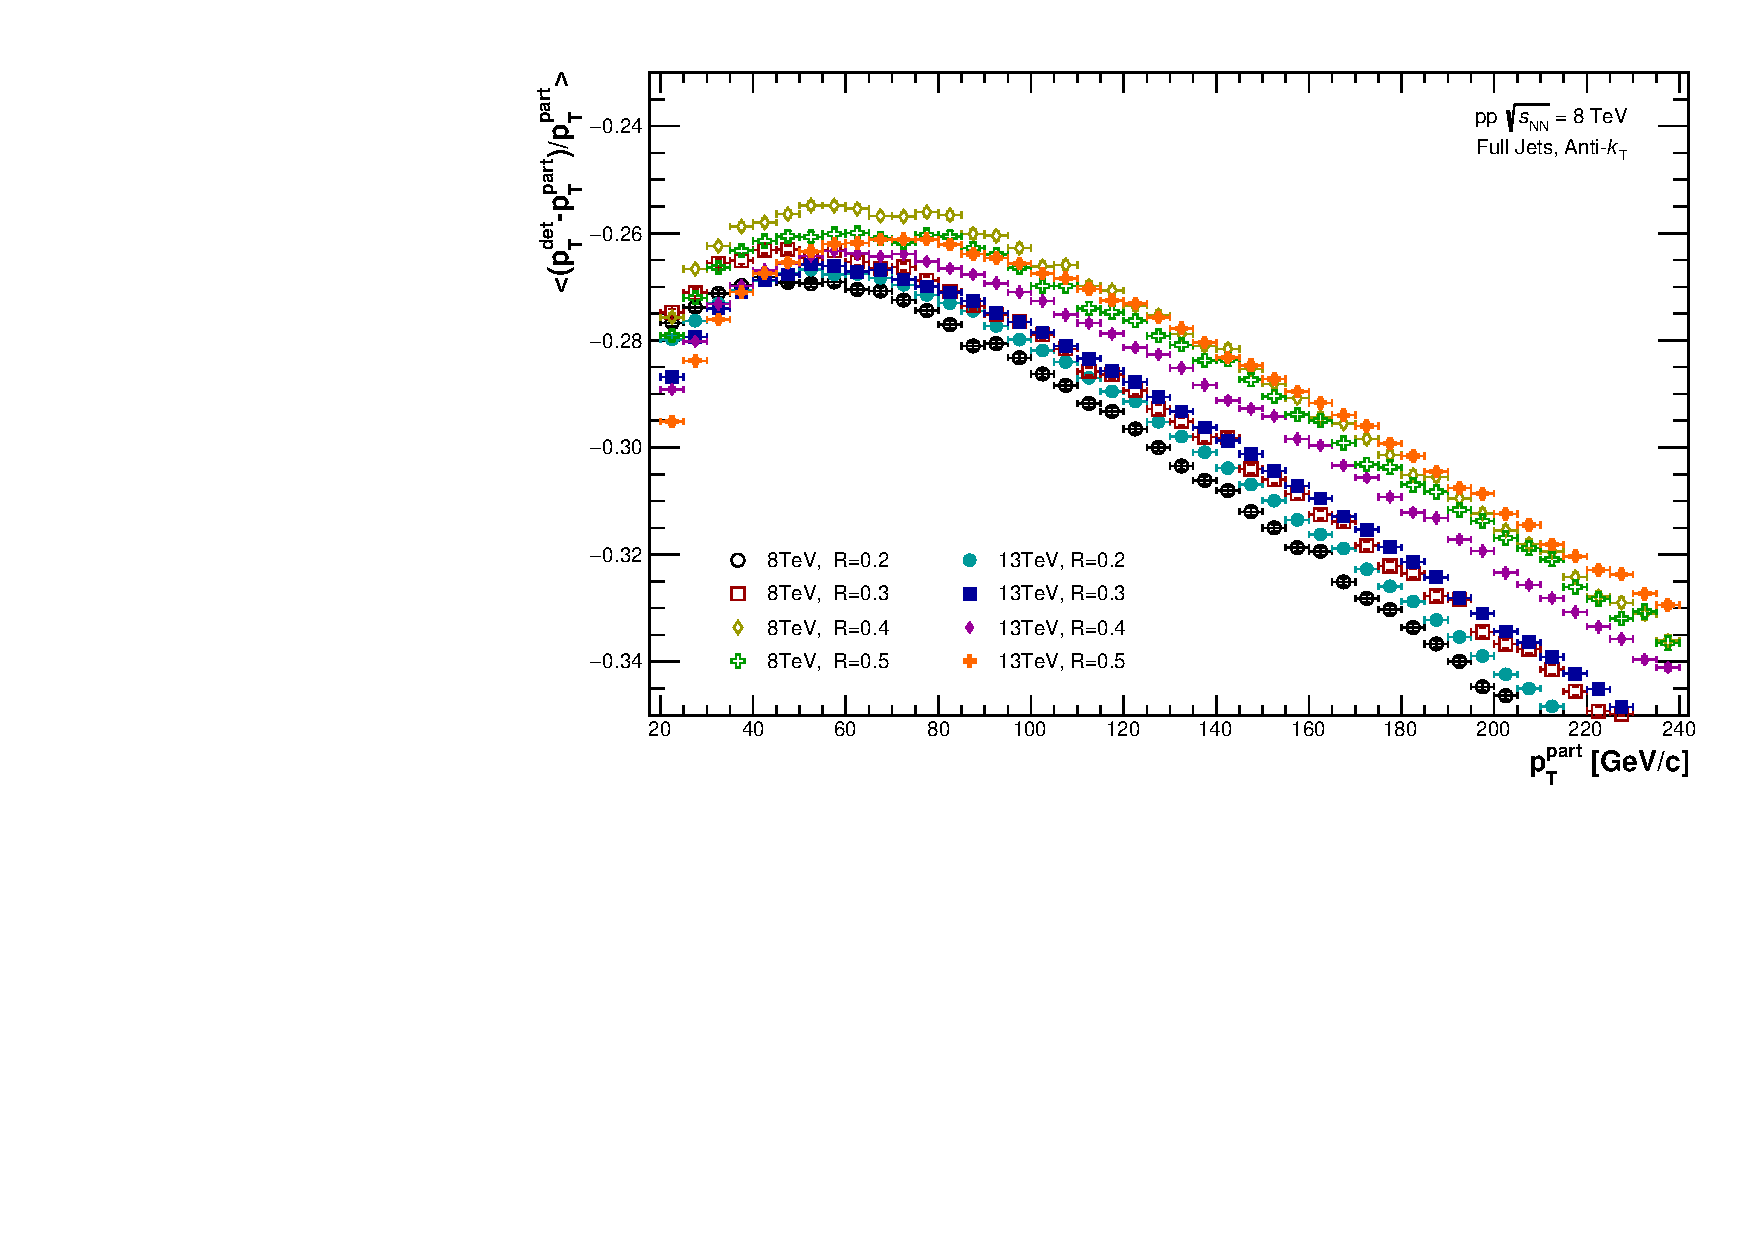
\includegraphics[width=7.5cm]{figures/EnergyScale/EnergyScaleMean_Comparison.pdf}
        \vfill\null 
        \columnbreak
            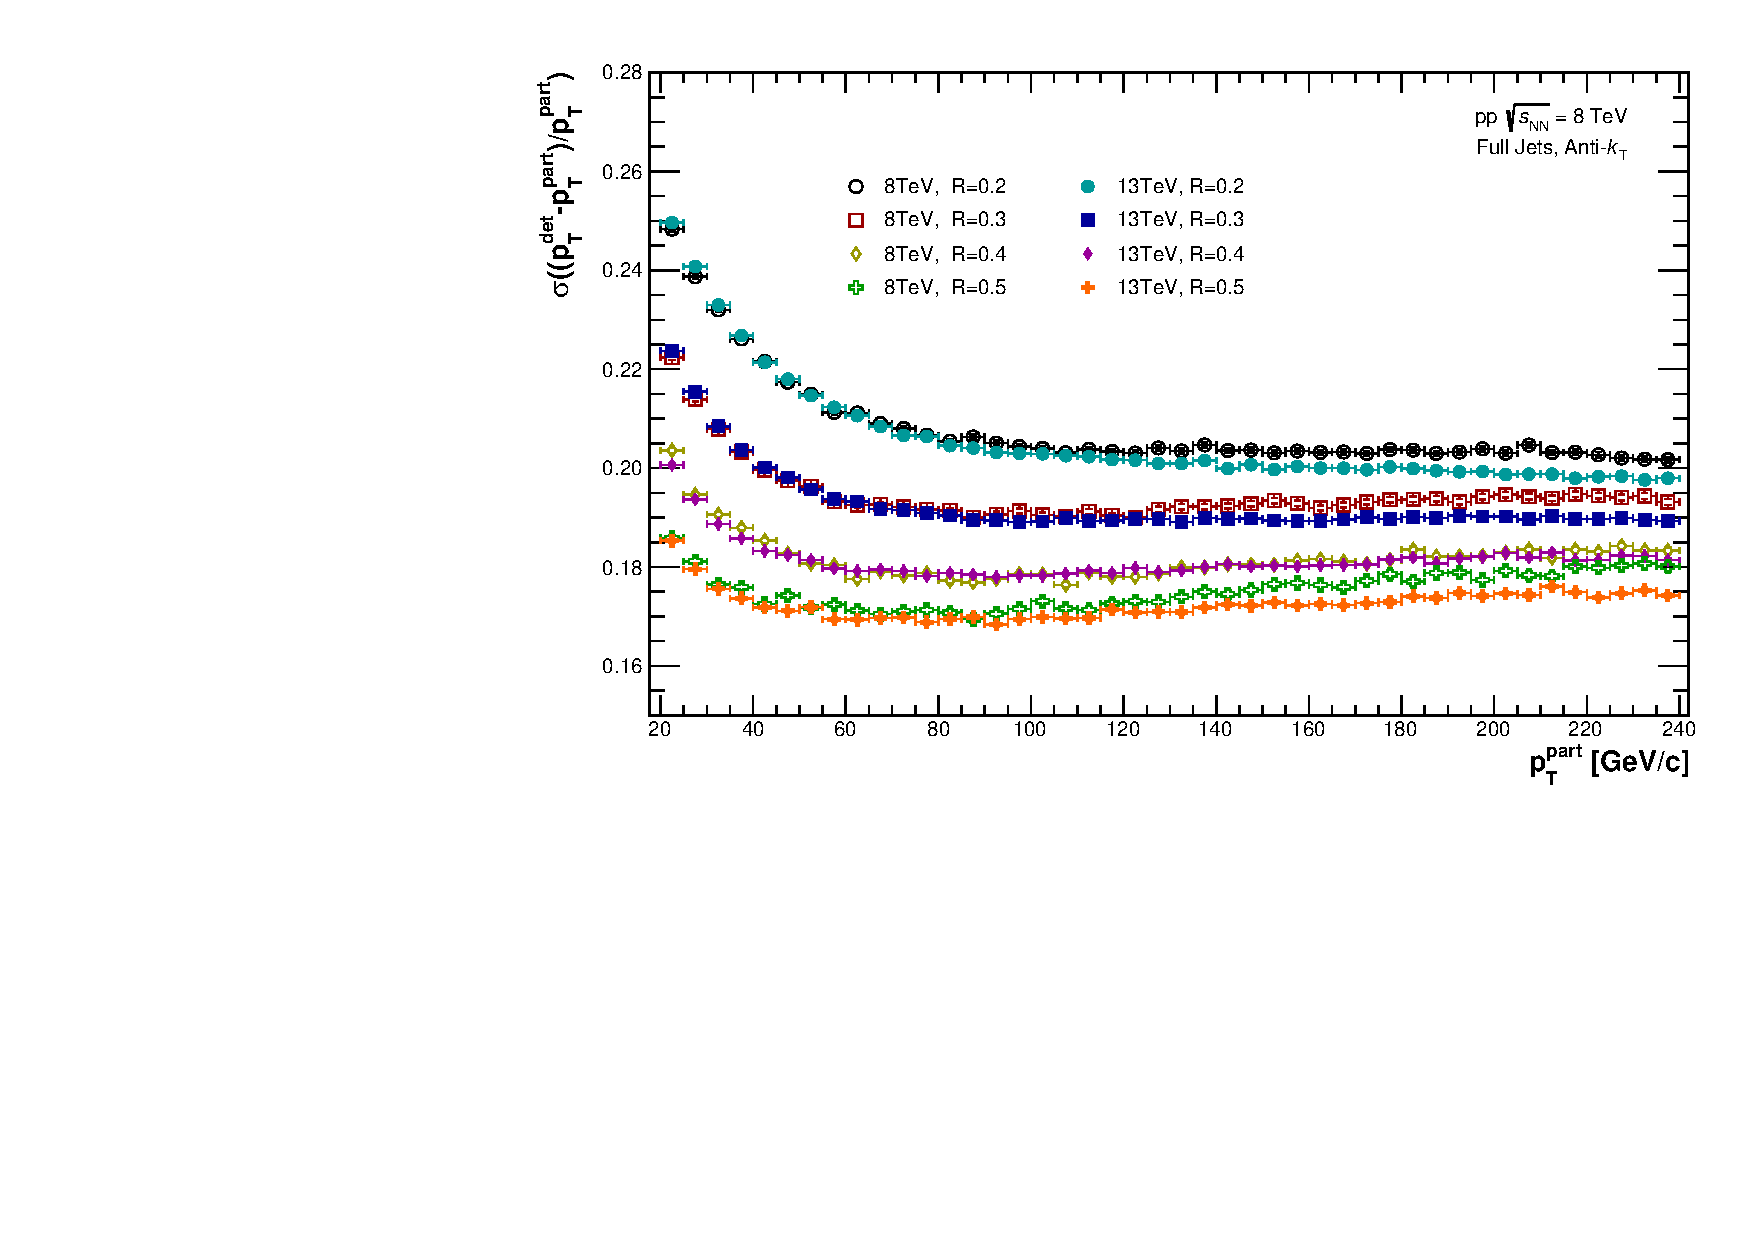
\includegraphics[width=7.5cm]{figures/EnergyScale/EnergyScaleWidth_Comparison.pdf}
        \vfill\null
    \end{multicols}
    \caption{Jet energy scale (left) and jet energy resolution (right) from the results of this analysis (\DIFaddbeginFL \pp \DIFaddendFL 8 TeV) compared to those of the \DIFaddbeginFL \pp \DIFaddendFL 13 TeV analysis.}
    \label{fig:EnergyScaleComp}
\end{figure}

A different R-ordering can also be seen when comparing the jet energy scale from 8 TeV and 13 TeV. For 13 TeV (and \DIFaddbegin \pp \DIFaddend 5 TeV), the energy scale increases with increasing radii from R = 0.2 - 0.6, whereas in 8 TeV, the energy scale increases from R = 0.2 - 0.4, then decreases again for R = 0.5 and R = 0.6. This has been studied, and a likely conclusion has been reached, but it is important to point out that although the jet energy scale ordering is different, it can be seen in figure \ref{fig:eScaleShapeWidth} that the shape of the distributions is comparable, but the width is slightly greater for 8 TeV.

\begin{figure}[h!]
    \centering
    \subfigure{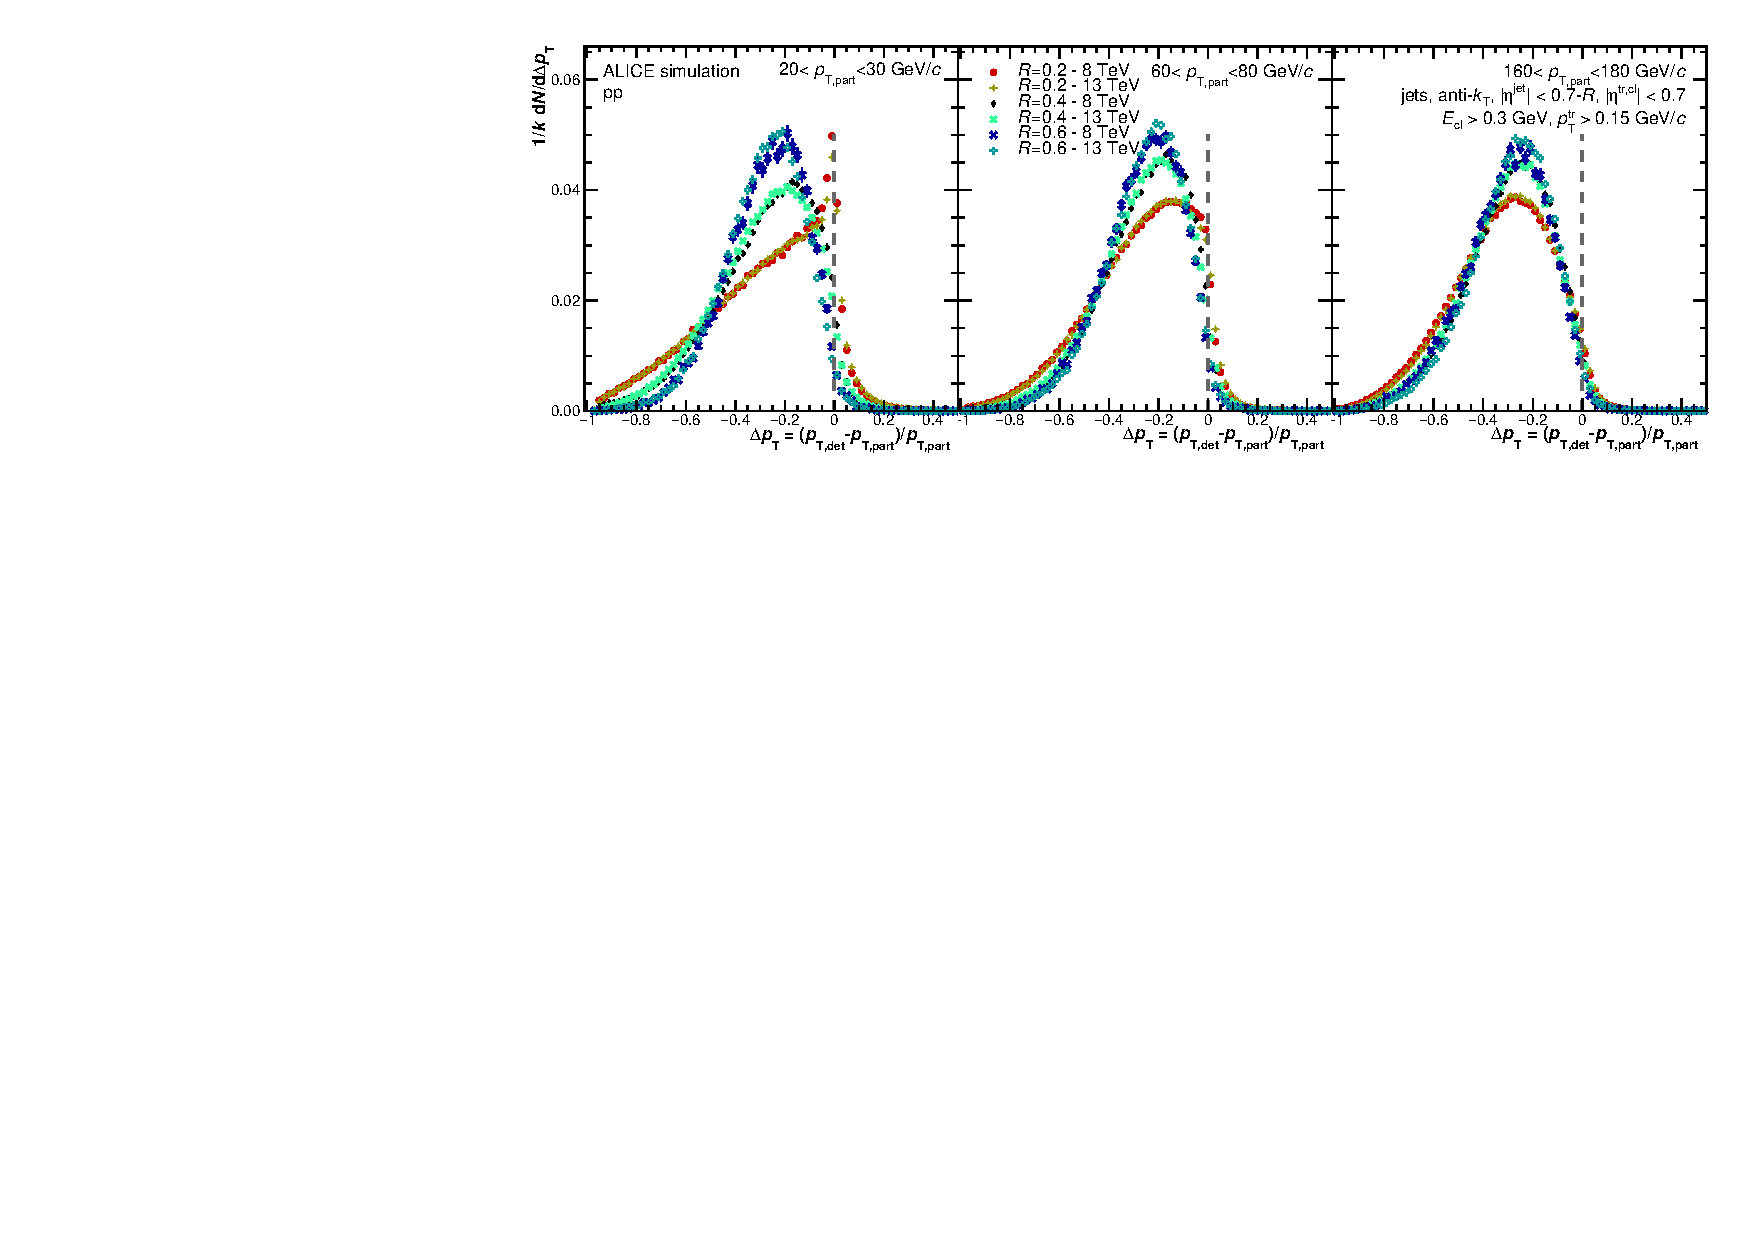
\includegraphics[width=0.85\textwidth]{figures/EnergyScale/ROrdering/JetEscaleProj_3_EnergyComp.pdf}}
    \subfigure{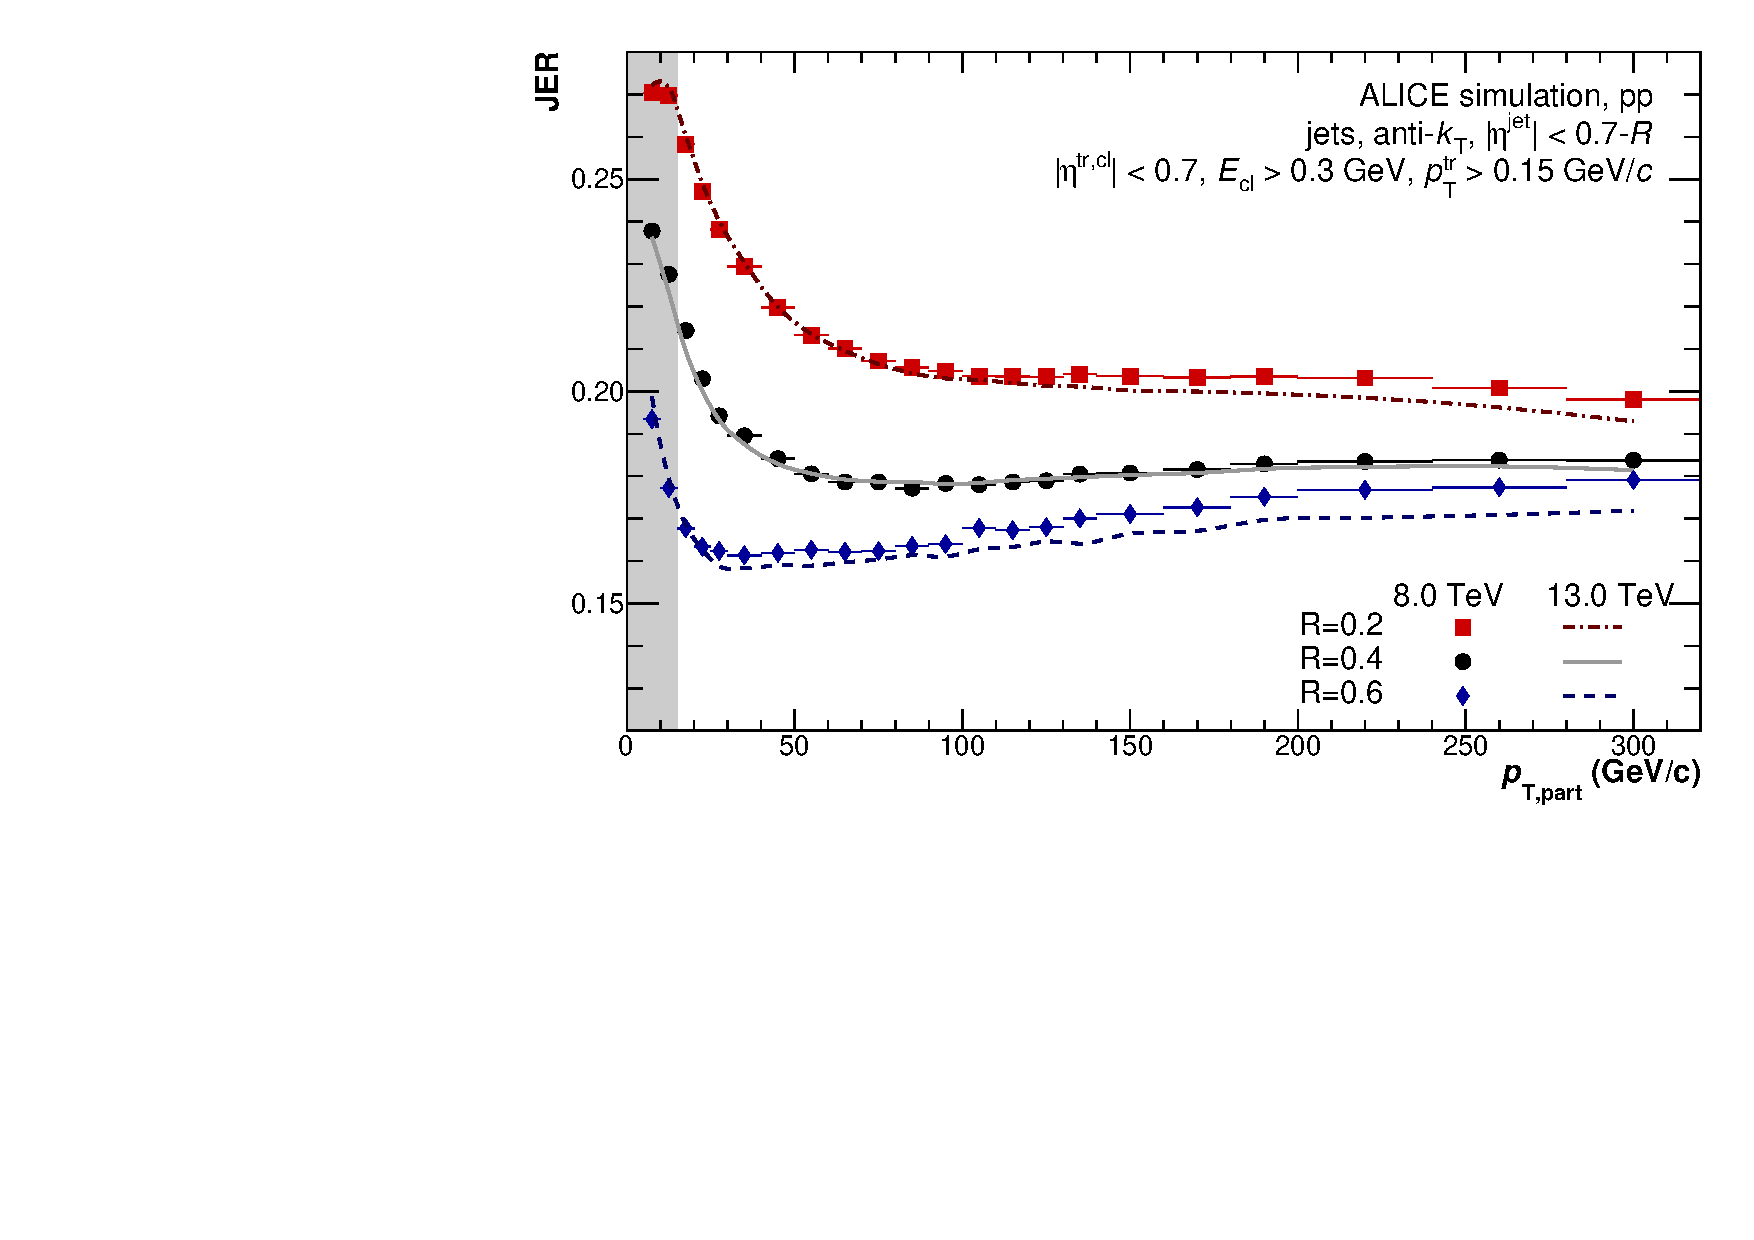
\includegraphics[width=0.75\textwidth]{figures/EnergyScale/ROrdering/JER_8_13_3_EnergyComp.pdf}}
    \caption{Jet energy scale projections showing the shape of the distributions (top), and the width of the residuals (bottom) for 8 and 13 TeV \DIFaddbeginFL \DIFaddFL{in }\pp \DIFaddFL{collisions}\DIFaddendFL .}
    \label{fig:eScaleShapeWidth}
\end{figure}

To explore the discrepancy, the jet energy scale is broken down into its charged and neutral components (figure \ref{fig:eScaleChNe}). The R-ordering difference is seen for both components, but is greater for the neutral component. For the charged component, in 2012, there were "holes" in the SPD tracking, and the ITS-TPC track matching was different as a function of phi. This was not present for the majority of the runs (evident by the smaller impact compared to the neutral component), but was enough to see an effect. For the neutral component, in 2012, the TRD was only partially installed. Some of the EMCal supermodules had TRD material in front of them, while others did not. The larger the jet radius, the more likely it was to cross boundaries in the EMCal between where there was and was not TRD material, or overlap with tracking holes in the ITS. Example plots showing tracking and EMCal occupancy as a function of $\eta$ and $\phi$ can be seen in figure \ref{fig:eScaleTracksClusters}.

\begin{figure}[h!]
    \centering
    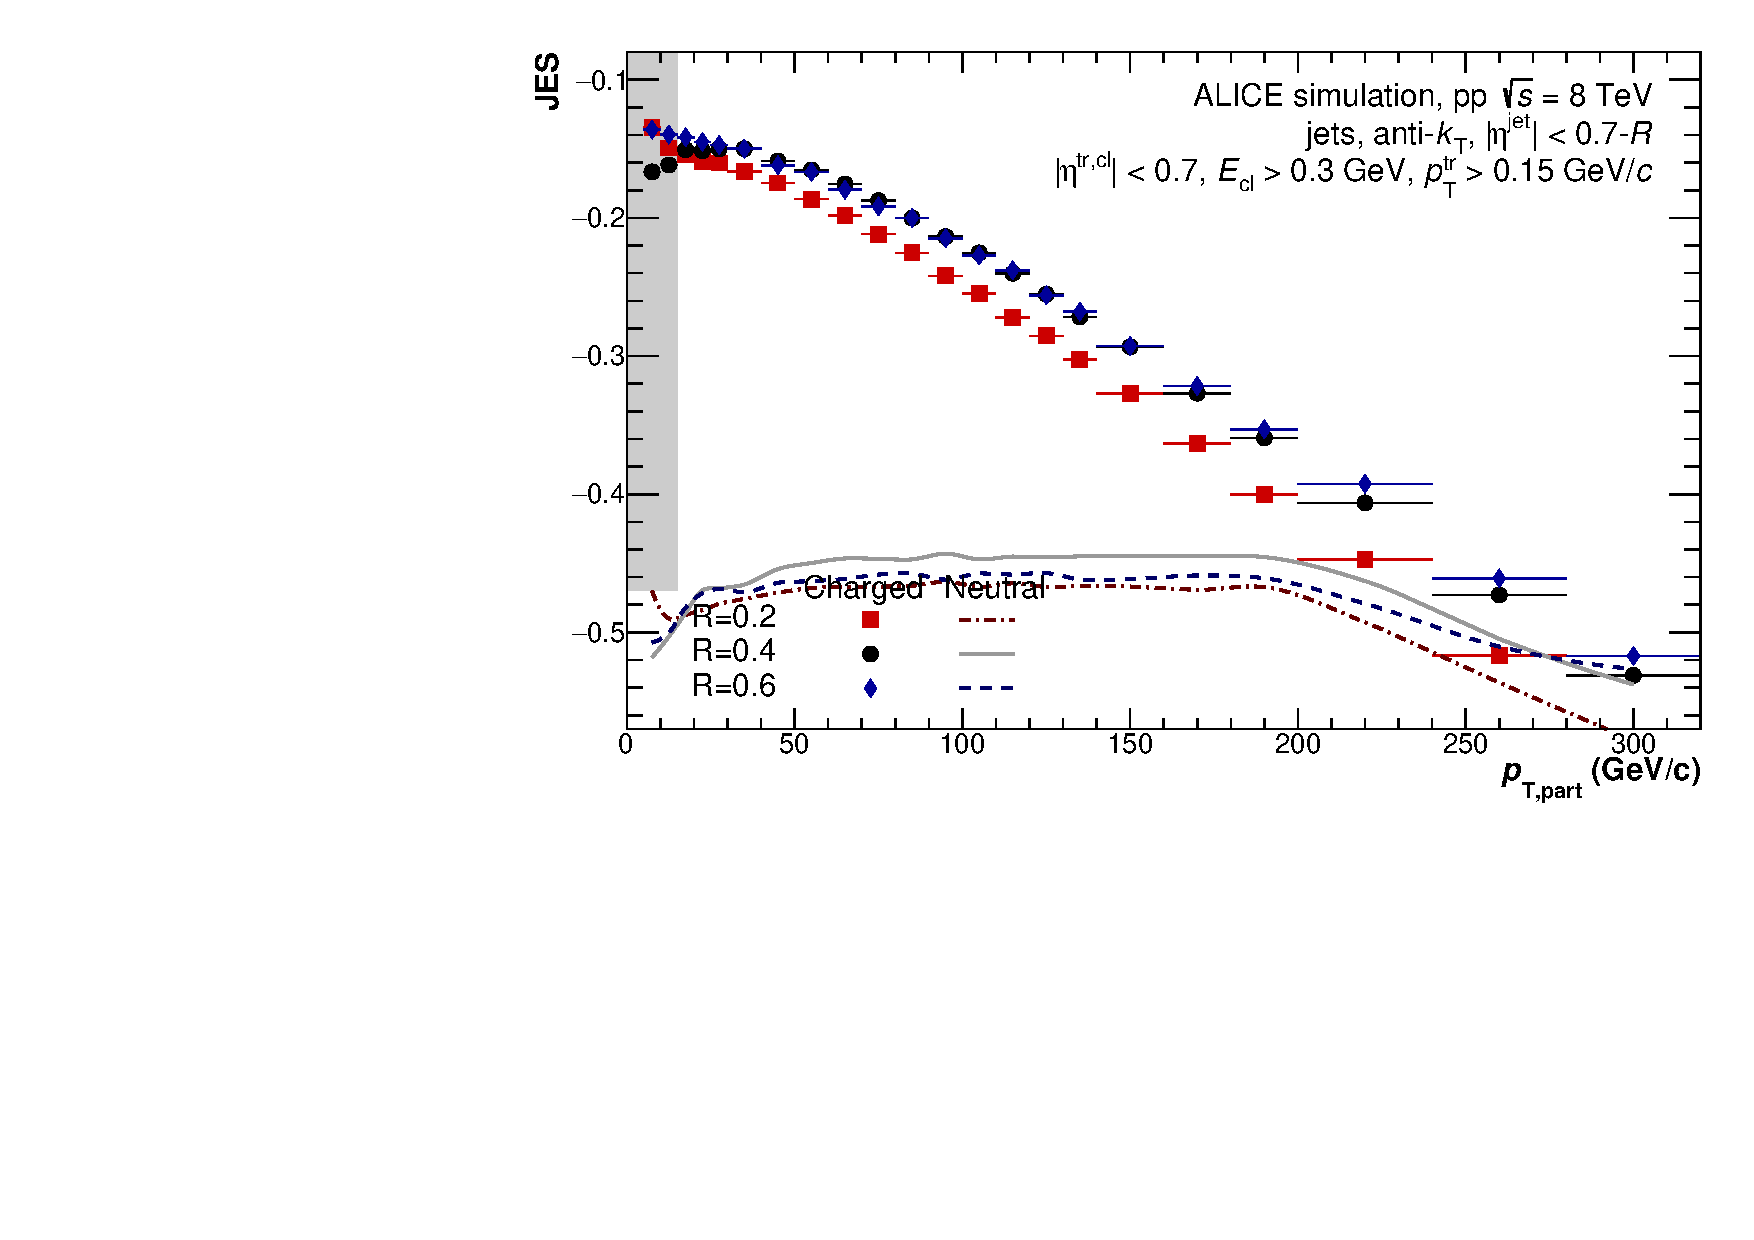
\includegraphics[width=0.75\textwidth]{figures/EnergyScale/ROrdering/JES_8_3_ChNe.pdf}
    \caption{Jet energy scale broken up into its charged and neutral components.}
    \label{fig:eScaleChNe}
\end{figure}

\begin{figure}[h!]
    \centering
    \subfigure{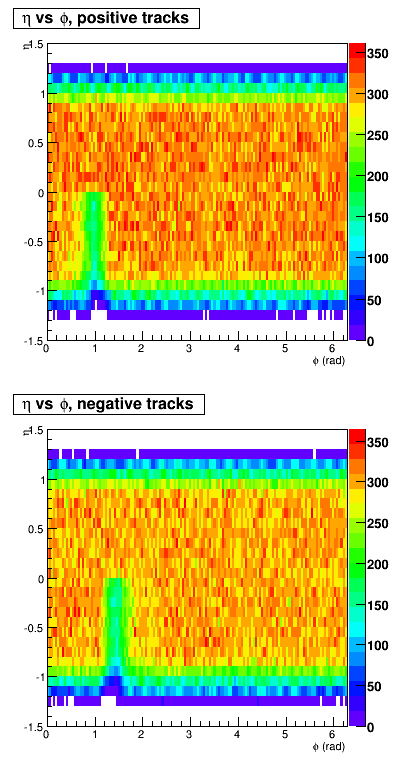
\includegraphics[width=0.25\textwidth]{figures/EnergyScale/ROrdering/spd_holes.png}}
    \subfigure{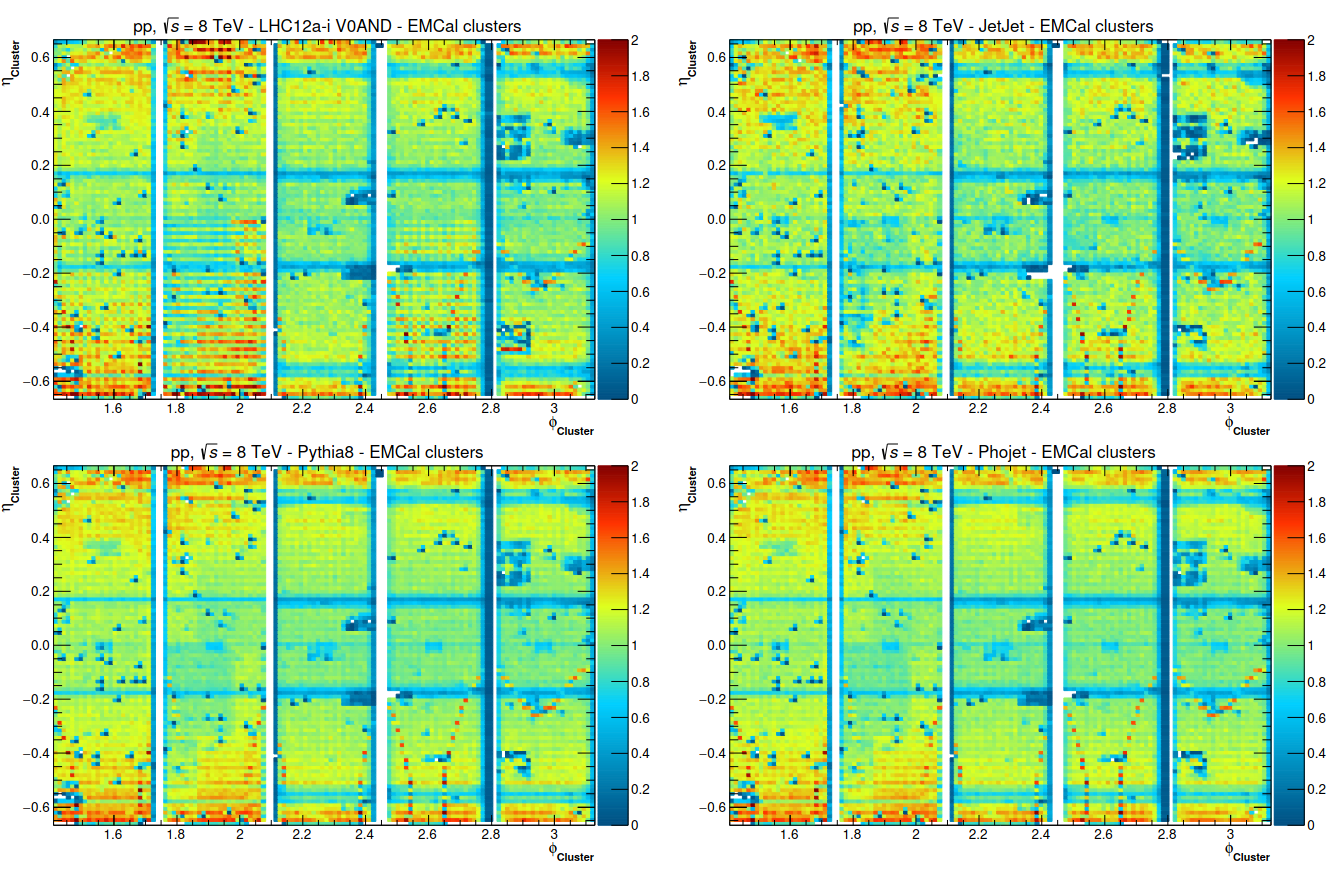
\includegraphics[width=0.73\textwidth]{figures/EnergyScale/ROrdering/emcal_occupancy.png}}
    \caption{TPC-ITS tracking (left) and EMCal occupancy (right) as a function of eta and phi.}
    \label{fig:eScaleTracksClusters}
\end{figure}
\clearpage{}
\clearpage{}\section{Jet Cross-Section Measurement and Corrections}
\label{chap:jetXsec}

\subsection{Jet Reconstruction and Selection}
\label{sec:JetRecoSel}

Jets are reconstructed with the fastjet package using the anti-k$_T$ algorithm under the E-scheme. Charged constituent tracks are measured with the central barrel tracking detectors TPC and ITS, and neutral constituents are measured with the EMCal. Tracks are selected using the standard hybrid track method with a minimum track p$_T$ of 150 MeV/c, excluding hybrid tracks failing refit in the ITS. EMCal clusters are reconstructed with the v3 clusterizer algorithm using an EMCal seed threshold of 300 MeV and a cell threshold of 100 MeV. These methods were also used in \cite{anaNoteMFasel}, and are standard for jet analyses. Only clusters with an energy larger than 300 MeV are considered, and the cluster energy is corrected for non-linearity using the final corrections stated in the recent EMCal performance paper \cite{EMCalPerformance2022}. This corresponds to kTestBeamShaper and kTestBeamFinalMC for data and monte carlo, respectively. In order to remove clusters from different bunch crossings within the EMCal integration window, a time cut of [-30,+35] ns is applied \DIFdelbegin \DIFdel{. This is the same cut }\DIFdelend \DIFaddbegin \DIFadd{for }\pp\DIFadd{, and a time cut of }[\DIFadd{\textcolor{red}{insert \pPb time cut}}] \DIFadd{ns is applied for }\pPb\DIFadd{. These are the cuts }\DIFaddend used within the GA group, and the same was followed here. Cluster energy measured before the event cannot be from the event, given a finite resolution. Cluster energy measured after the event can be from slower particles. In order to avoid double counting of energy deposited by charged particles in the EMCal, the contribution from all tracks matched to clusters is estimated and subtracted from the cluster energy using momentum-dependent track matching. So-called exotic clusters, i.e clusters with a very high percentage of energy deposited in a single cell, are removed from the analysis. Jets at detector level are required to be fully contained within the EMCal acceptance and have a minimum pt of 10 GeV/c. As the study covers a \DIFdelbegin \DIFdel{pt }\DIFdelend \DIFaddbegin \pT \DIFaddend range exceeding 100 GeV/c, tracks with constituent p$_T$ up to 200 GeV/c are accepted in order to not introduce a fragmentation bias. It should be noted that tracks with a \DIFdelbegin \DIFdel{p\mbox{%DIFAUXCMD
$_T$
}%DIFAUXCMD
}\DIFdelend \DIFaddbegin \pT \DIFaddend larger than 100 GeV/c have a significantly worse \DIFdelbegin \DIFdel{p\mbox{%DIFAUXCMD
$_T$
}%DIFAUXCMD
}\DIFdelend \DIFaddbegin \pT \DIFaddend resolution. This is accounted for in the systematic uncertainities by varying the maximum track \pT.

\DIFaddbegin \subsection{\DIFadd{Background subtraction}}
\label{sec:backgroundSubtraction}

\DIFadd{\textcolor{red}{This would probably be a good place to stick the section about background subtraction.}
}

\DIFaddend \subsection{Trigger normalization and correction for the rejection factor}
\label{sec:triggerCorrection}

\begin{figure}
    \centering
    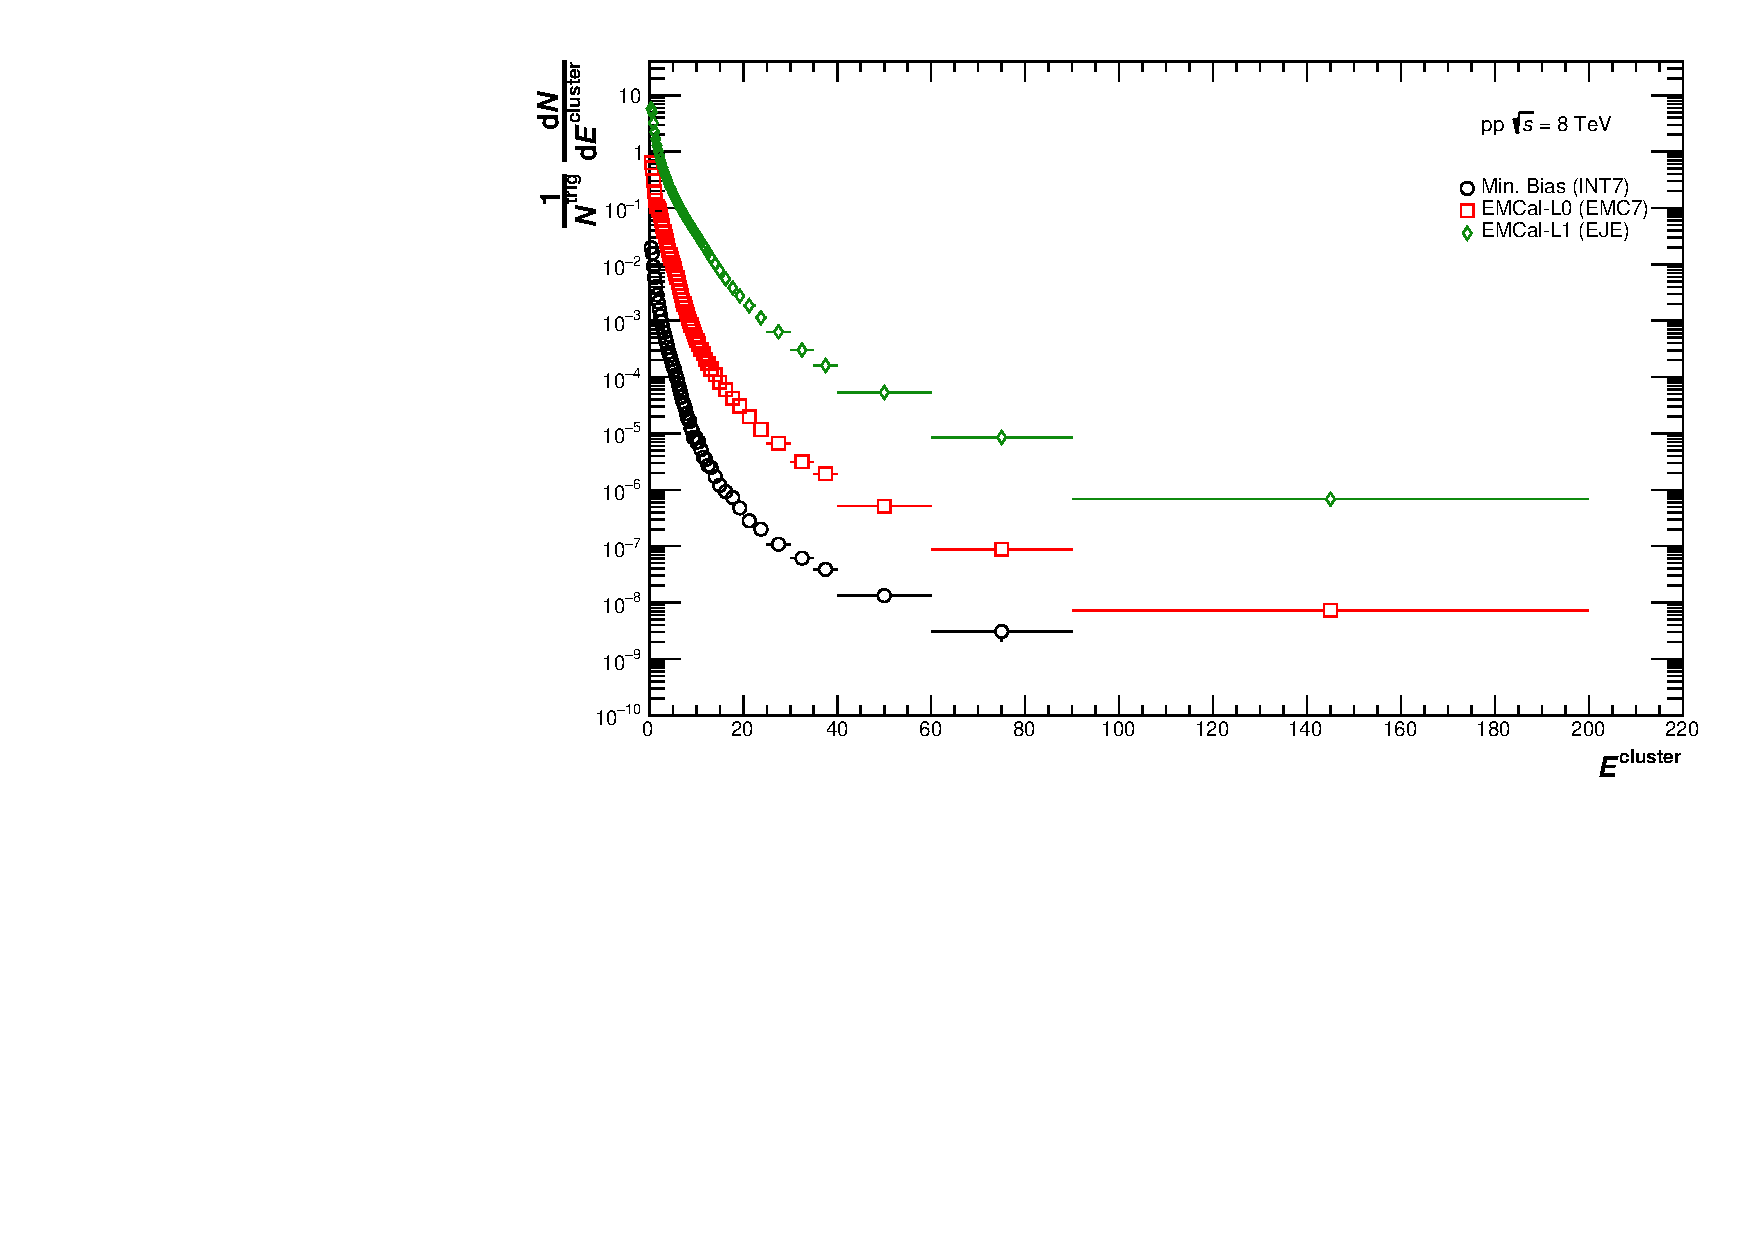
\includegraphics[width=15cm]{figures/TriggerClusters/clusters_R02.pdf}
    \caption{Trigger cluster yields for the INT7, EMC7, and EJE triggers \DIFaddbeginFL \DIFaddFL{in }\pp \DIFaddFL{(left), and for INT7, EJ2, and EJ1 triggers in }\pPb \DIFaddFL{(right) \textcolor{red}{insert \pPb trigger cluster plot}}\DIFaddendFL . Rejection factors are required in order for the spectra to overlap.}
    \label{fig:triggerClusters}
\end{figure}

The trigger cluster yield for all three triggers for jet radius R = 0.2 can be found in \ref{fig:triggerClusters}. The integrated luminosity inspected by the trigger is independent of the probe, therefore it is sufficient to study only one jet radius. From this, it can be seen that the yields do not overlap. This is due to the downscaling of the minimum bias\DIFdelbegin \DIFdel{and EMCal-L0 }\DIFdelend \DIFaddbegin \DIFadd{, EMC7, and EJ2 }\DIFaddend triggers (to different degrees) in order to allow trigger time for the EMCal triggers to record rare events (jets, in this case). In the 2012 dataset, these downscale factors were not recorded. Instead, the triggered data must be corrected by the use of rejection factors. \DIFaddbegin \DIFadd{The downscale factors were recorded for the 2016 }\pPb \DIFadd{dataset, but rejection factors are also used here in order to achieve equivalence with the }\pp \DIFadd{measurement. }\DIFaddend These trigger rejection factors are calculated by taking the ratio of the trigger cluster yield between triggers with neighboring thresholds after correction for the cluster trigger efficiency. In this case, the ratio is taken between the EMC7 \DIFaddbegin \DIFadd{(EJ2) }\DIFaddend and INT7 triggers and between the EJE \DIFaddbegin \DIFadd{(EJ1) }\DIFaddend and EMC7 \DIFaddbegin \DIFadd{(EJ2) }\DIFaddend triggers. The EMC7 \DIFaddbegin \DIFadd{(EJ2) }\DIFaddend trigger is then divided by the former, while the EJE \DIFaddbegin \DIFadd{(EJ1) }\DIFaddend trigger is divided by both rejection factors. The ratio of cluster yields for different triggers without correction for the cluster trigger efficiency is shown in figure \ref{fig:RejectionFactorsUnscaled}. The plateaus are fit with an error function, and the flat region of the function is taken as the constant rejection factor. The ratio of cluster yields for different triggers after the trigger efficiency correction is shown in figure \ref{fig:RejectionFactors}. The plateaus are fit linearly to find the rejection factor.

\begin{figure}
    \centering
    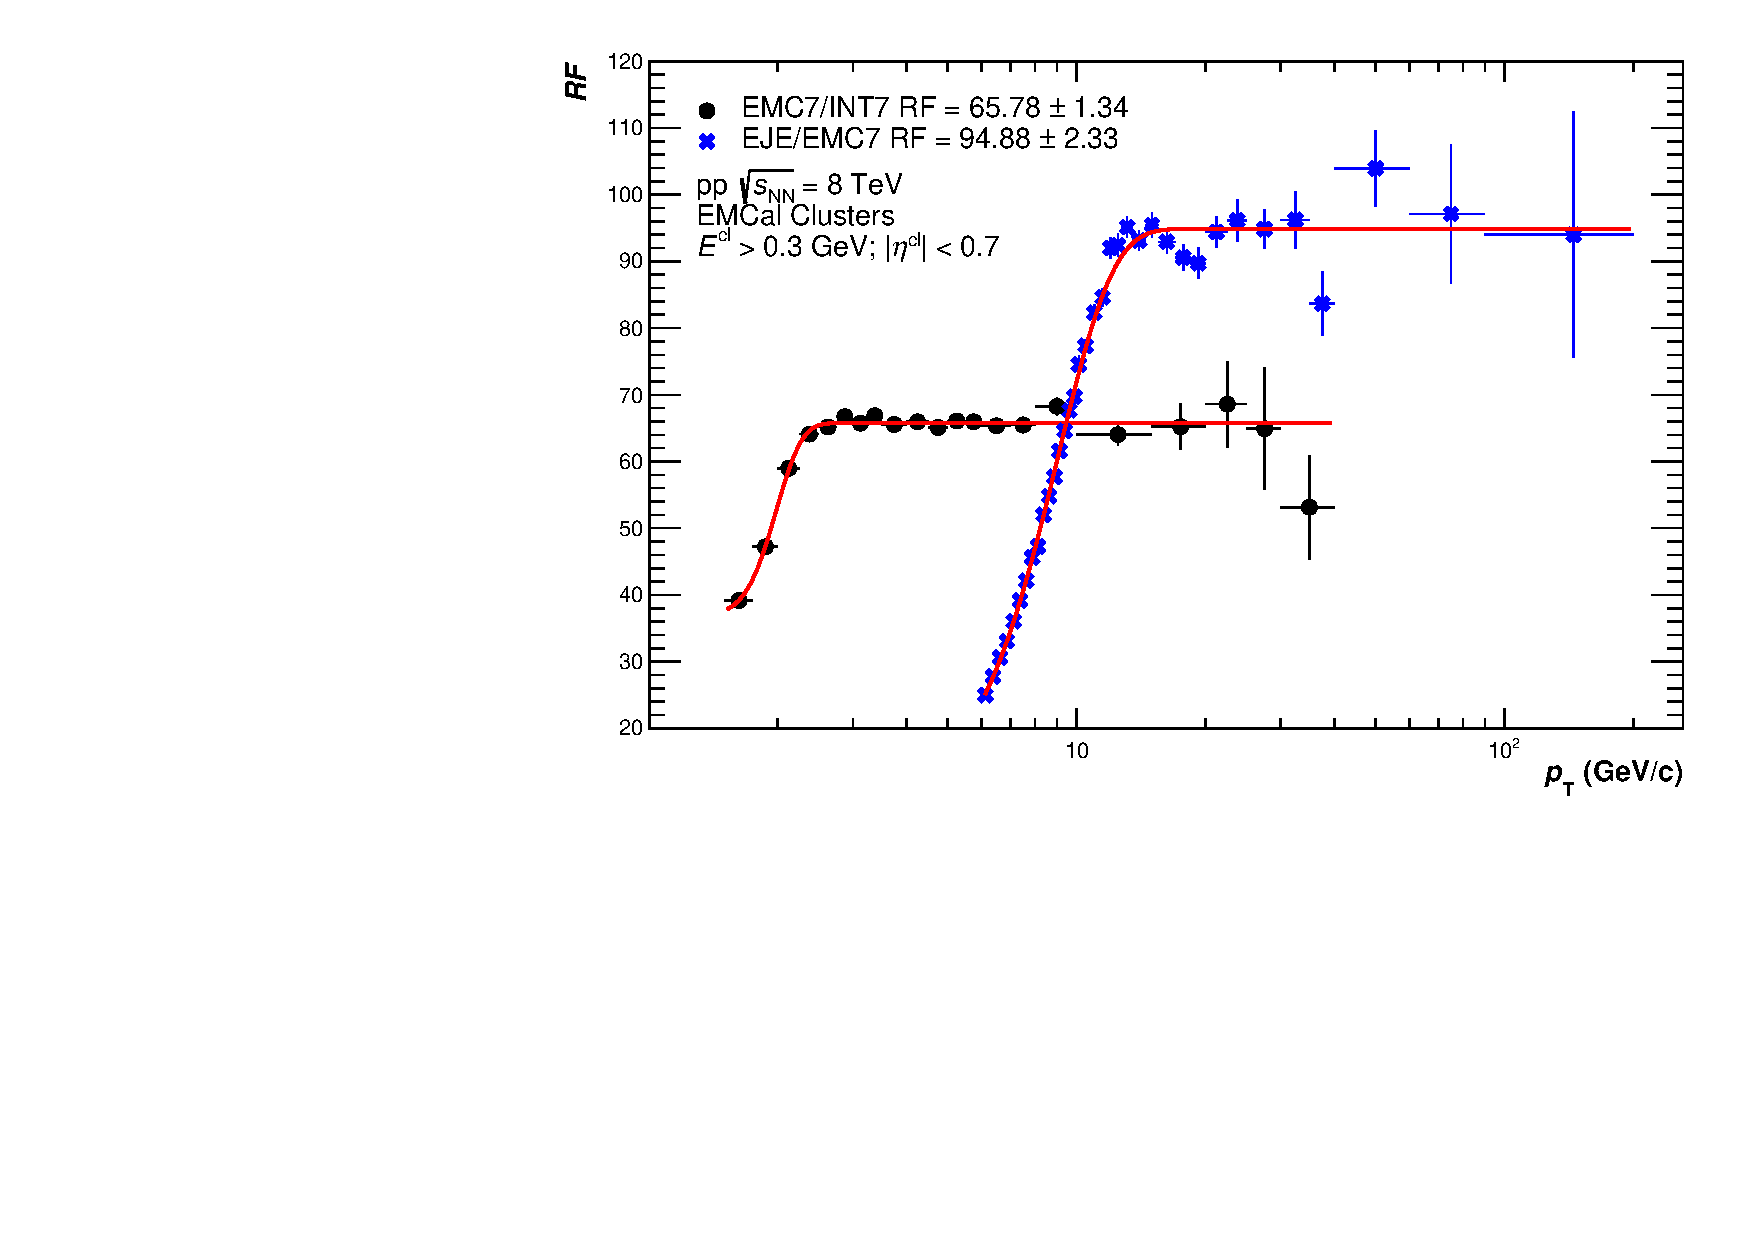
\includegraphics[width=15cm]{figures/RejectionFactors/RF_R02_Unscaled.pdf}
    \caption{Rejection factors for the EMC7 trigger and the EJE trigger \DIFaddbeginFL \DIFaddFL{(left) and for the EJ2 and EJ1 triggers (right) \textcolor{red}{insert RF plot}}\DIFaddendFL , found by taking the ratio of the event-normalized trigger yields of the EMC7/INT7 \DIFaddbeginFL \DIFaddFL{(EJ2/INT7) }\DIFaddendFL triggers and EJE/EMC7 \DIFaddbeginFL \DIFaddFL{(EJ1/EJ2) }\DIFaddendFL triggers, respectively.}
    \label{fig:RejectionFactorsUnscaled}
\end{figure}

\begin{figure}
    \centering
    \includegraphics[width=15cm]{figures/RejectionFactors/RF_R02.pdf}
    \caption{Rejection factors scaled by the cluster trigger efficiency \DIFaddbeginFL \DIFaddFL{in }\pp \DIFaddFL{(left) and }\pPb \DIFaddFL{(right) \textcolor{red}{insert RF plot}}\DIFaddendFL .}
    \label{fig:RejectionFactors}
\end{figure}

\subsection{Combination of the triggers at raw level}
\label{sec:triggerCombination}

\begin{figure}
    \centering
    \begin{multicols}{2}
            \includegraphics[width=7.5cm]{figures/CorrRawSpec/corrRawSpec_INT7.pdf}
            \includegraphics[width=7.5cm]{figures/CorrRawSpec/corrRawSpec_EMC7.pdf}
        \vfill\null 
        \columnbreak
            \includegraphics[width=7.5cm]{figures/CorrRawSpec/corrRawSpec_EJE.pdf}
        \vfill\null
    \end{multicols}
    \caption{Raw spectra for the three triggers with corrections from chapter \ref{chap:TriggerAndInstrumentation} for varous jet radii.}
    \label{fig:CorrRawSpec}
\end{figure}

The raw spectrum is constructed by combining the raw spectra from the three trigger classes after the application of the rejection factors and the corrections discussed in chapter \ref{chap:TriggerAndInstrumentation}. Fig. \ref{fig:CorrRawSpec} shows the comparison of the raw spectra from the three triggers \DIFaddbegin \DIFadd{in }\pp \DIFaddend for jets with different jet radii. 

As can be seen in section \ref{sec:EMCTriggerBias}, figure \ref{fig:trigger_ratios}, the ratio EMC7/INT7 (EJE/EMC7) deviates from 1 for jets with pt $>$ 30 (60) GeV/c. As discussed in chapter \ref{sec:EMCTriggerBias}, jets with \pT $<$ 30 (60) GeV/c for the the EMC7 (EJE) trigger also suffer from effects like random noise, which are not simulated, contributing to triggers selecting jets in the sub-threshold region. The trigger efficiency is therefore underestimated in this \pT region and the corrections cannot be trusted any more. For the combination of the spectra at raw level, the data points from the triggers are selected in a way that contributes the least to the statistical uncertainty. The ranges are selected as the following:

\begin{itemize}
    \item 20 GeV/c $\le$ \pT $<$ 30 GeV/c: INT7 trigger
    \item 30 GeV/c $\le$ \pT $<$ 60 GeV/c: EMC7 trigger
    \item \pT $\ge$ 60 GeV/c: EJE trigger
\end{itemize}

These ranges are chosen based on the topics discussed in section \ref{sec:ptRanges}. Additionally, at very high momentum, energy corrections - in particular with respect to the non-linearity in EMCal - are not sufficiently well understood to perform a measurement.

\DIFaddbegin \DIFadd{The same is true for the triggers in }\pPb\DIFadd{, and the ranges for these triggers are selected as the following:
}

\begin{itemize}
    \item \DIFadd{\textcolor{red}{?} GeV/c \mbox{%DIFAUXCMD
$\le$
}%DIFAUXCMD
}\pT \DIFadd{\mbox{%DIFAUXCMD
$<$
}%DIFAUXCMD
\textcolor{red}{?} GeV/c: INT7 trigger
    }\item \DIFadd{30 GeV/c \mbox{%DIFAUXCMD
$\le$
}%DIFAUXCMD
}\pT \DIFadd{\mbox{%DIFAUXCMD
$<$
}%DIFAUXCMD
\textcolor{red}{?} GeV/c: EJ2 trigger
    }\item \pT \DIFadd{\mbox{%DIFAUXCMD
$\ge$
}%DIFAUXCMD
\textcolor{red}{?} GeV/c: EJ1 trigger
}\end{itemize}

\DIFaddend \subsection{Cross section normalization}
\label{sec:xsecNomalization}

Since the jet yield was measured only in the EMCal acceptance, a correction for the limited acceptance has to be applied. The acceptance correction is

\begin{equation}
    Acc = \frac{\Delta\eta \Delta\phi}{2\pi}
\end{equation}

where $\Delta\eta$ = 1.4 − 2R and $\Delta\phi$ = 1.745 − 2R.

\DIFaddbegin \DIFadd{\textcolor{red}{Check to see if this changed for 2016 b/c of extra emcal modules}
}

\DIFaddend The number of events has to be corrected for the vertex finding efficiency. The vertex finding efficiency is defined as the fraction of events before and after vertex selection and is evaluated before the vertex-z cut. The vertex finding efficiency has been determined from the event counters for accepted and rejected events to be 94.8$\%$ for INT7, 99.2$\%$ for EMC7, \DIFdelbegin \DIFdel{and }\DIFdelend 99.6$\%$ for EJE, \DIFaddbegin \DIFadd{\textcolor{red}{?}\mbox{%DIFAUXCMD
$\%$
}%DIFAUXCMD
for EJ2, and \textcolor{red}{?}\mbox{%DIFAUXCMD
$\%$
}%DIFAUXCMD
for EJ1, }\DIFaddend and applied as scaling factor to the spectrum. EMCal triggered events have a higher multiplicity on average, so there are more tracks to reconstruct the vertex with, especially in pp-collisions.

The reference cross section for the INT7 trigger (V0AND condition) has been determined in a van-der-Meer scan to be 55.8 mb \DIFdelbegin \DIFdel{, }\DIFdelend with an uncertainty of 2.6$\%$ \DIFaddbegin \DIFadd{in }\pp\DIFadd{, and \textcolor{red}{?} mb with an uncertainty of \textcolor{red}{?}\mbox{%DIFAUXCMD
$\%$
}%DIFAUXCMD
in }\pPb\DIFaddend . The total correction excluding unfolding is

\begin{equation}
   \frac{d\sigma}{dp_T d\eta} = \frac{\sigma_{V0AND}\epsilon_{vtx}}{N_{trg,INT7}} \frac{1}{Acc\epsilon_{trg}*RF} \frac{dN_{jet}}{dp_T d\eta}
\end{equation}

with the corrected trigger yield N$_{trg,INT7}$, the vertex finding efficiency $\epsilon_{vtx}$, the trigger efficiency $\epsilon_{trg}$, and the rejection factor RF, which is 1 for the INT7 trigger. The corrected raw spectrum for different jet radii before unfolding is shown in fig. \ref{fig:CombinedRawSpec}

\begin{figure}
    \centering
    \includegraphics[width=15cm]{figures/CorrRawSpec/corrRawSpec_Combined.pdf}
    \vfill\null
    \caption{Combined raw spectrum after corrections for the rejection factors, vertex finding efficiency, trigger efficiency, and cross-section normalization \DIFaddbeginFL \DIFaddFL{for }\pp \DIFaddFL{(left) and }\pPb \DIFaddFL{(right) \textcolor{red}{insert combined \pPb spectra}}\DIFaddendFL .}
    \label{fig:CombinedRawSpec}
\end{figure}

\DIFaddbegin \subsection{\DIFadd{Embedding}}
\label{sec:embedding}

\DIFadd{\textcolor{red}{This would probably be a good place to stick the section about embedding.}
}

\DIFaddend \subsection{Unfolding of the jet spectrum}
\label{sec:unfolding}
\subsubsection{Kinematic efficiency}
\label{subsec:kinEff}

\begin{figure}
    \centering
    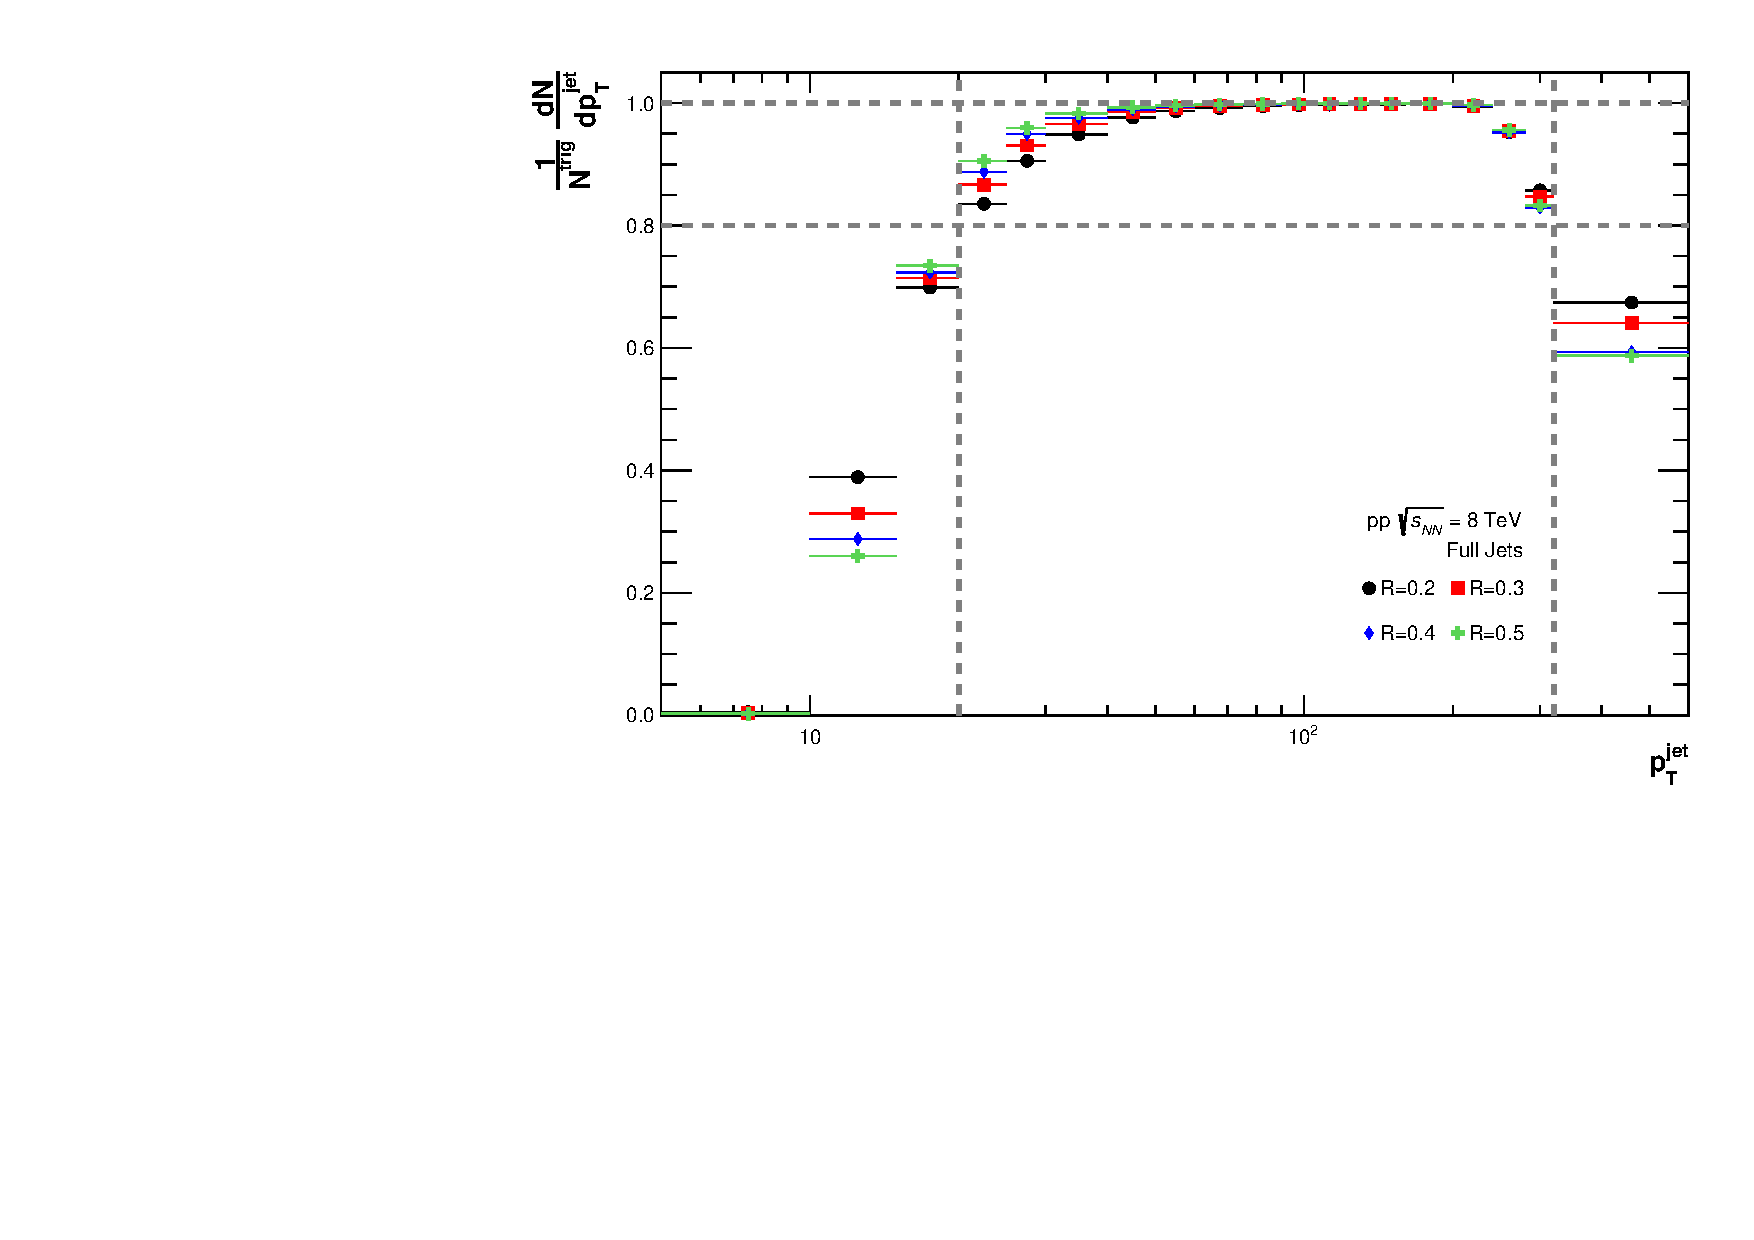
\includegraphics[width=15cm]{figures/KinematicEfficiency/EffKine.pdf}
    \caption{Kinematic efficiency for various jet radii \DIFdelbeginFL \DIFdelFL{.}\DIFdelendFL \DIFaddbeginFL \DIFaddFL{in }\pp \DIFaddFL{(left) and }\pPb \DIFaddFL{(right) \textcolor{red}{insert \pPb plot}}\DIFaddendFL }
    \label{fig:KinematicEfficiency}
\end{figure}

Fig. \ref{fig:KinematicEfficiency} shows the kinematic efficiency for jets with R=0.2 to R=0.6. Jets are selected at detector level to have a \pT within 10 and 240 GeV/c \DIFaddbegin \DIFadd{\textcolor{red}{see if this holds for \pPb, or if I NEED to keep it the same for consistency}}\DIFaddend . The efficiency is 80$\%$ beyond 20 GeV/c \DIFaddbegin \DIFadd{\textcolor{red}{check for \pPb}}\DIFaddend , and stays around this value in the whole region covered by the measurement. At lower \pT, the turn-on is sharper for jets with larger jet radii. The kinematic efficiency is corrected for in the unfolding procedure. A measurement is feasible for 20 GeV /c $<$ \pT $<$ 320 GeV/c \DIFaddbegin \DIFadd{\textcolor{red}{check if this holds}}\DIFaddend , where the reported range is selected where the kinematic efficiency is larger than 80$\%$.

\subsubsection{Unfolding tests \DIFaddbegin \DIFadd{- }\pp\DIFaddend }
\label{subsec:unfoldingTests}

For this measurement, both bayesian unfolding and unfolding based on singular value decomposition (SVD) are used. Both methods were implemented in the RooUnfold framework \cite{roounfold}. The bayesian method is used as the standard method, while SVD unfolding is used to test the sensitivity with respect to different unfolding methods. It is important to note that the unfolding procedure corrects towards harder spectra. The following figures contain test results for jet radius R = 0.2 for SVD and Bayesian unfolding. For the remaining jet radii, see appendix \ref{sec:AppendixUnfoldingTests}.

\begin{figure}
    \centering
    \begin{multicols}{2}
            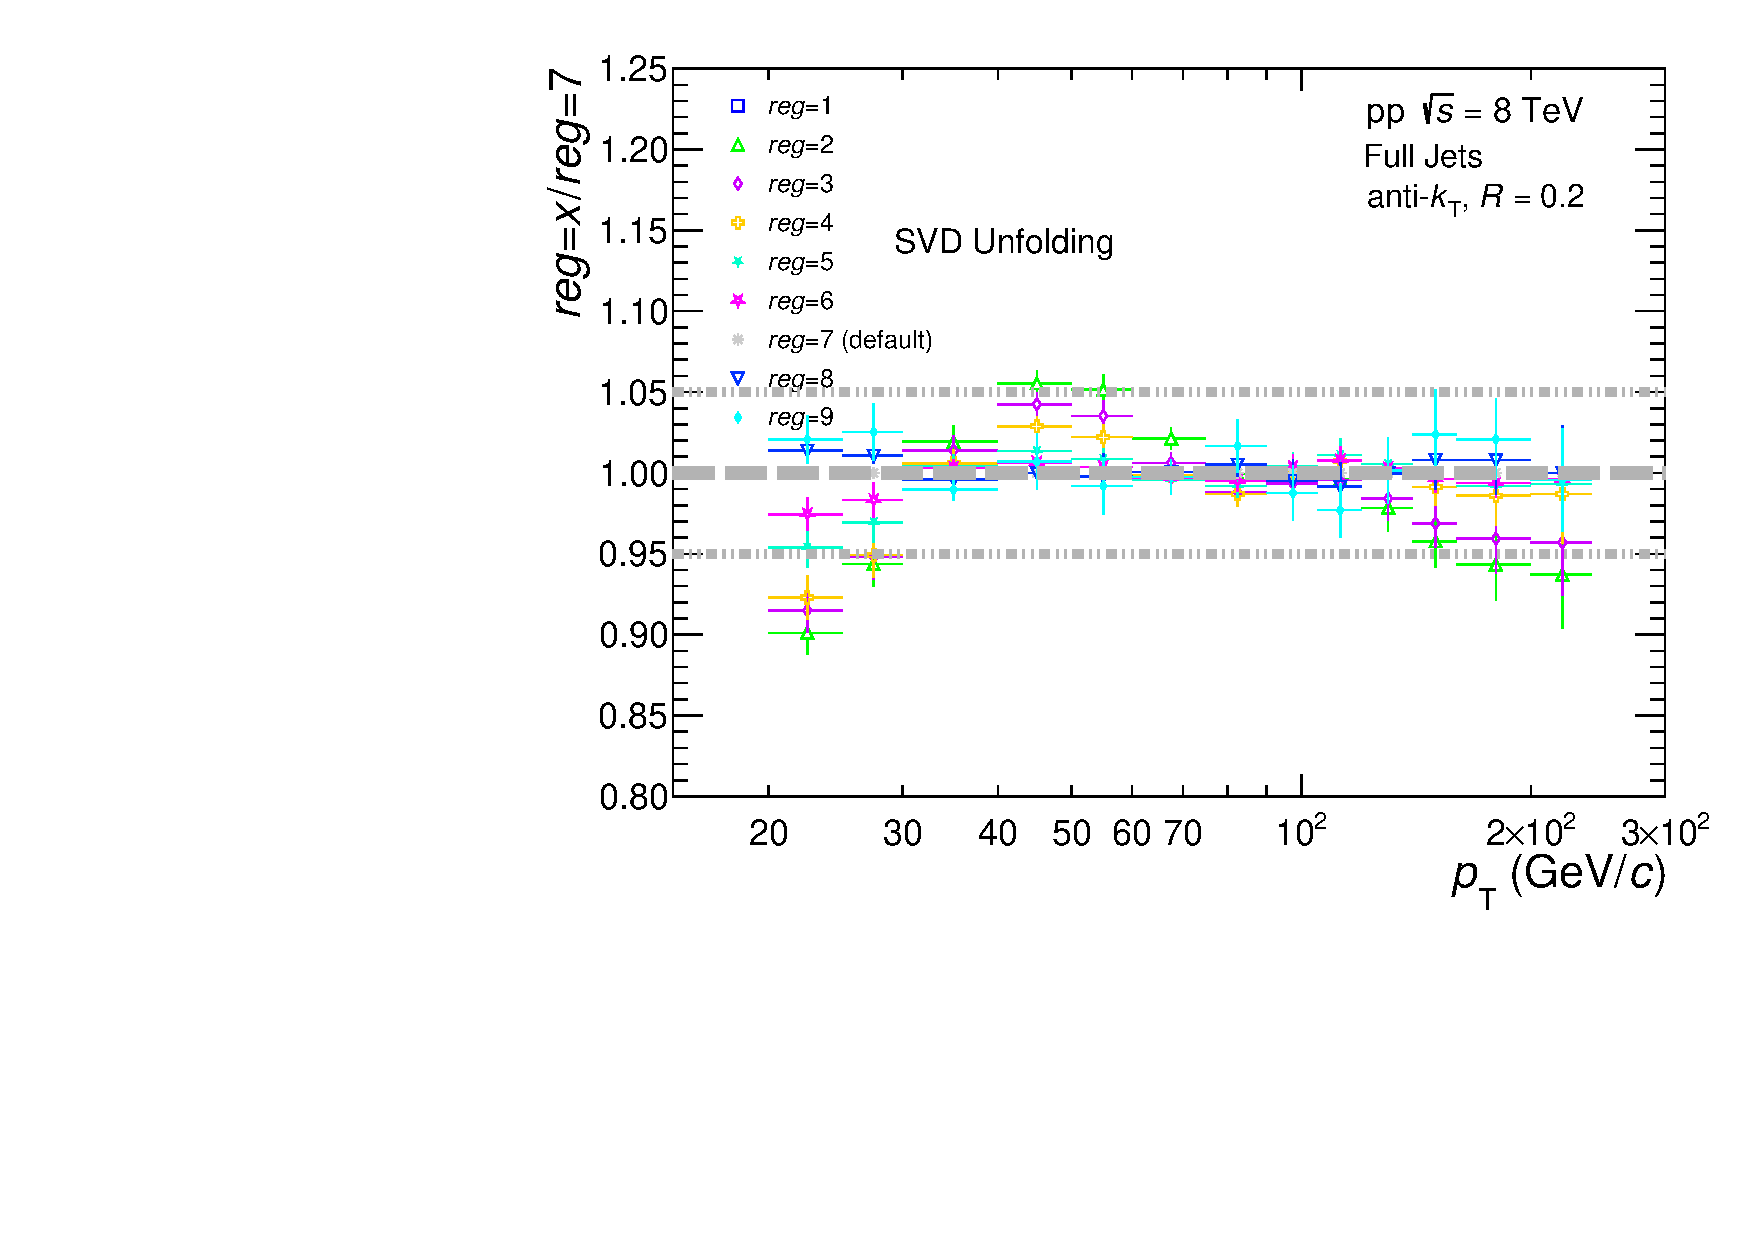
\includegraphics[width=7.5cm]{figures/UnfoldingComparisons/Regularizations/RatioRegularizationSvd_R02.pdf}
        \vfill\null 
        \columnbreak
            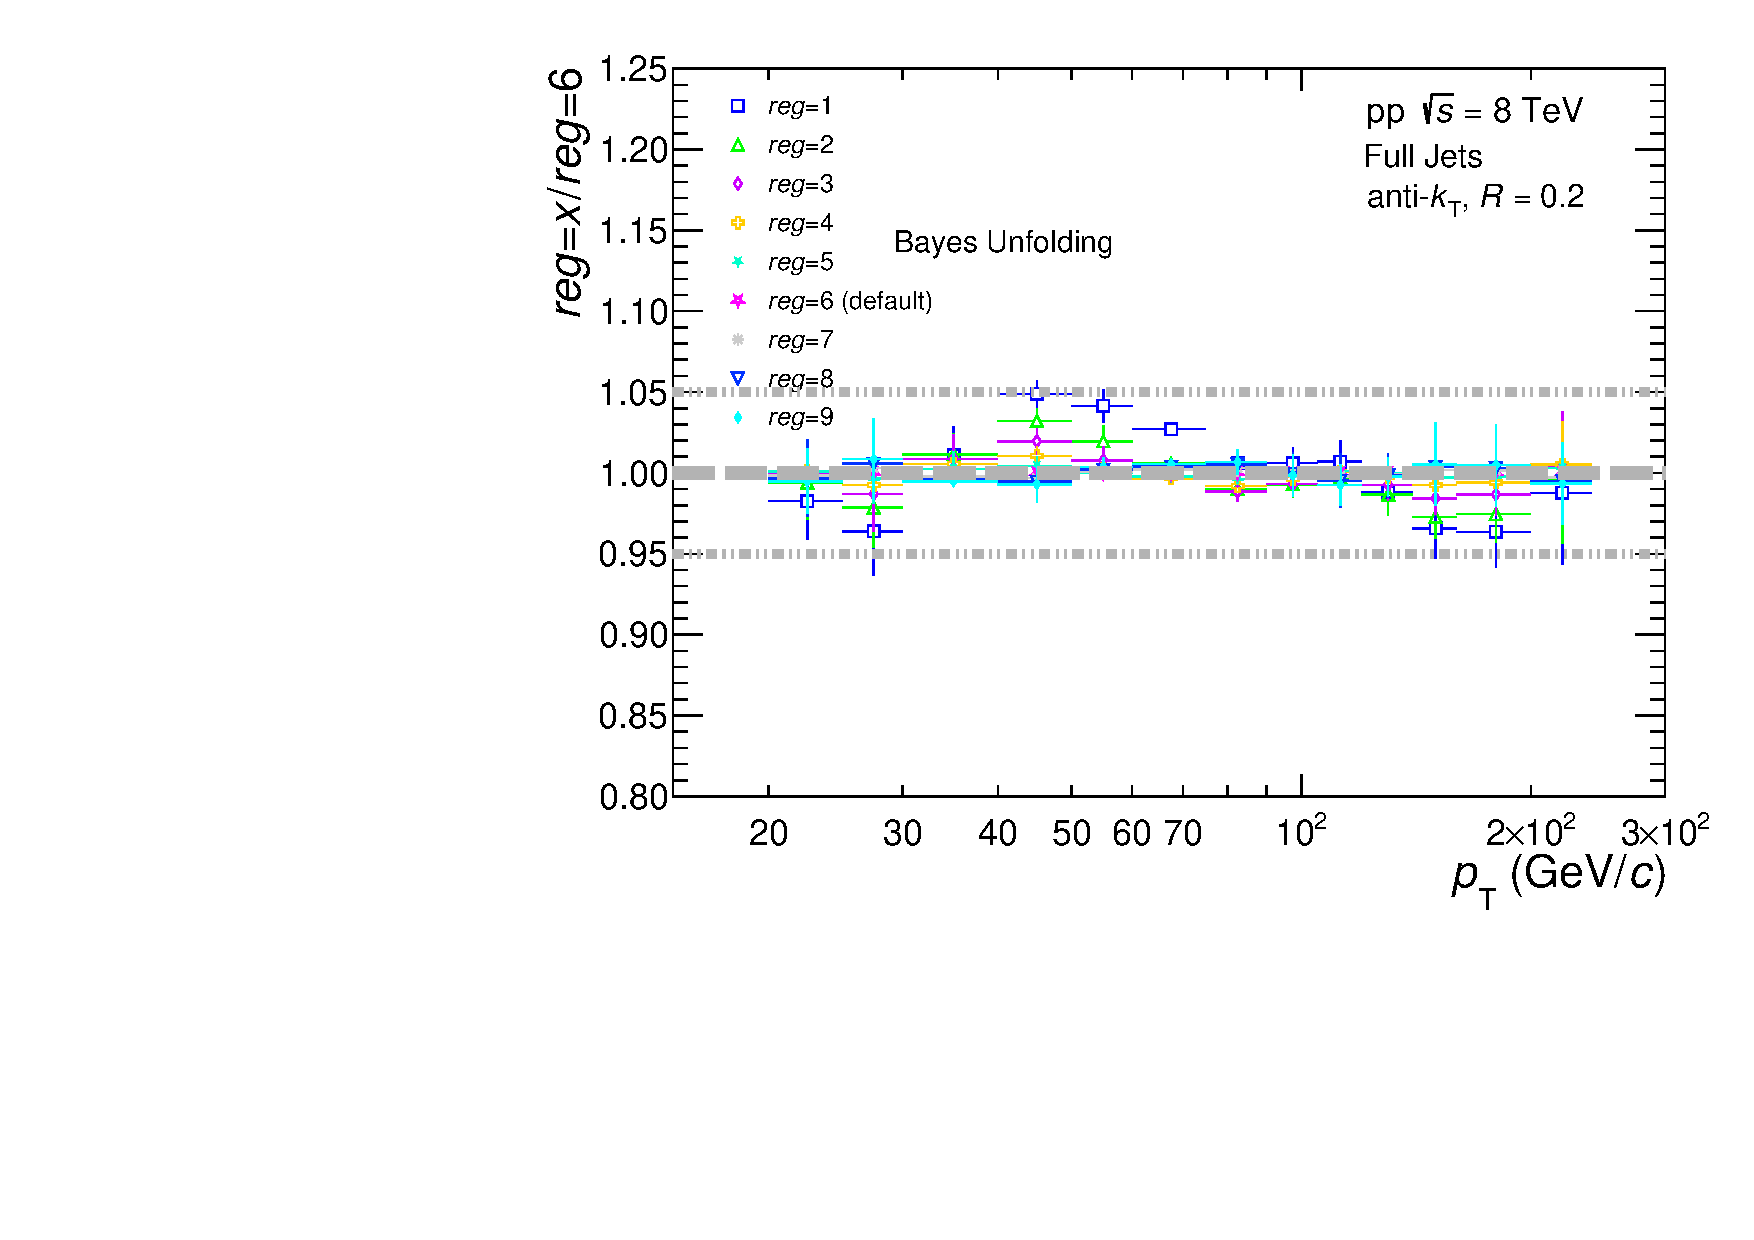
\includegraphics[width=7.5cm]{figures/UnfoldingComparisons/Regularizations/RatioRegularizationBayes_R02.pdf}
        \vfill\null
    \end{multicols}
    \caption{Regularization dependence for SVD (left) and Bayesian (right) unfolding.}
    \label{fig:RegIter}
\end{figure}

Fig. \ref{fig:RegIter} shows the dependence of the SVD and bayesian undfolded solutions on the regularization parameter. A regularization parameter of 7 is selected as default for the SVD unfolding, while for bayesian unfolding, 6 iterations is chosen as default with 4 and 9 as variations. The choice of the regularization parameter for SVD of 7 is also motivated by the D-vector (Fig. \ref{fig:DVector}). 

\begin{figure}
    \centering
    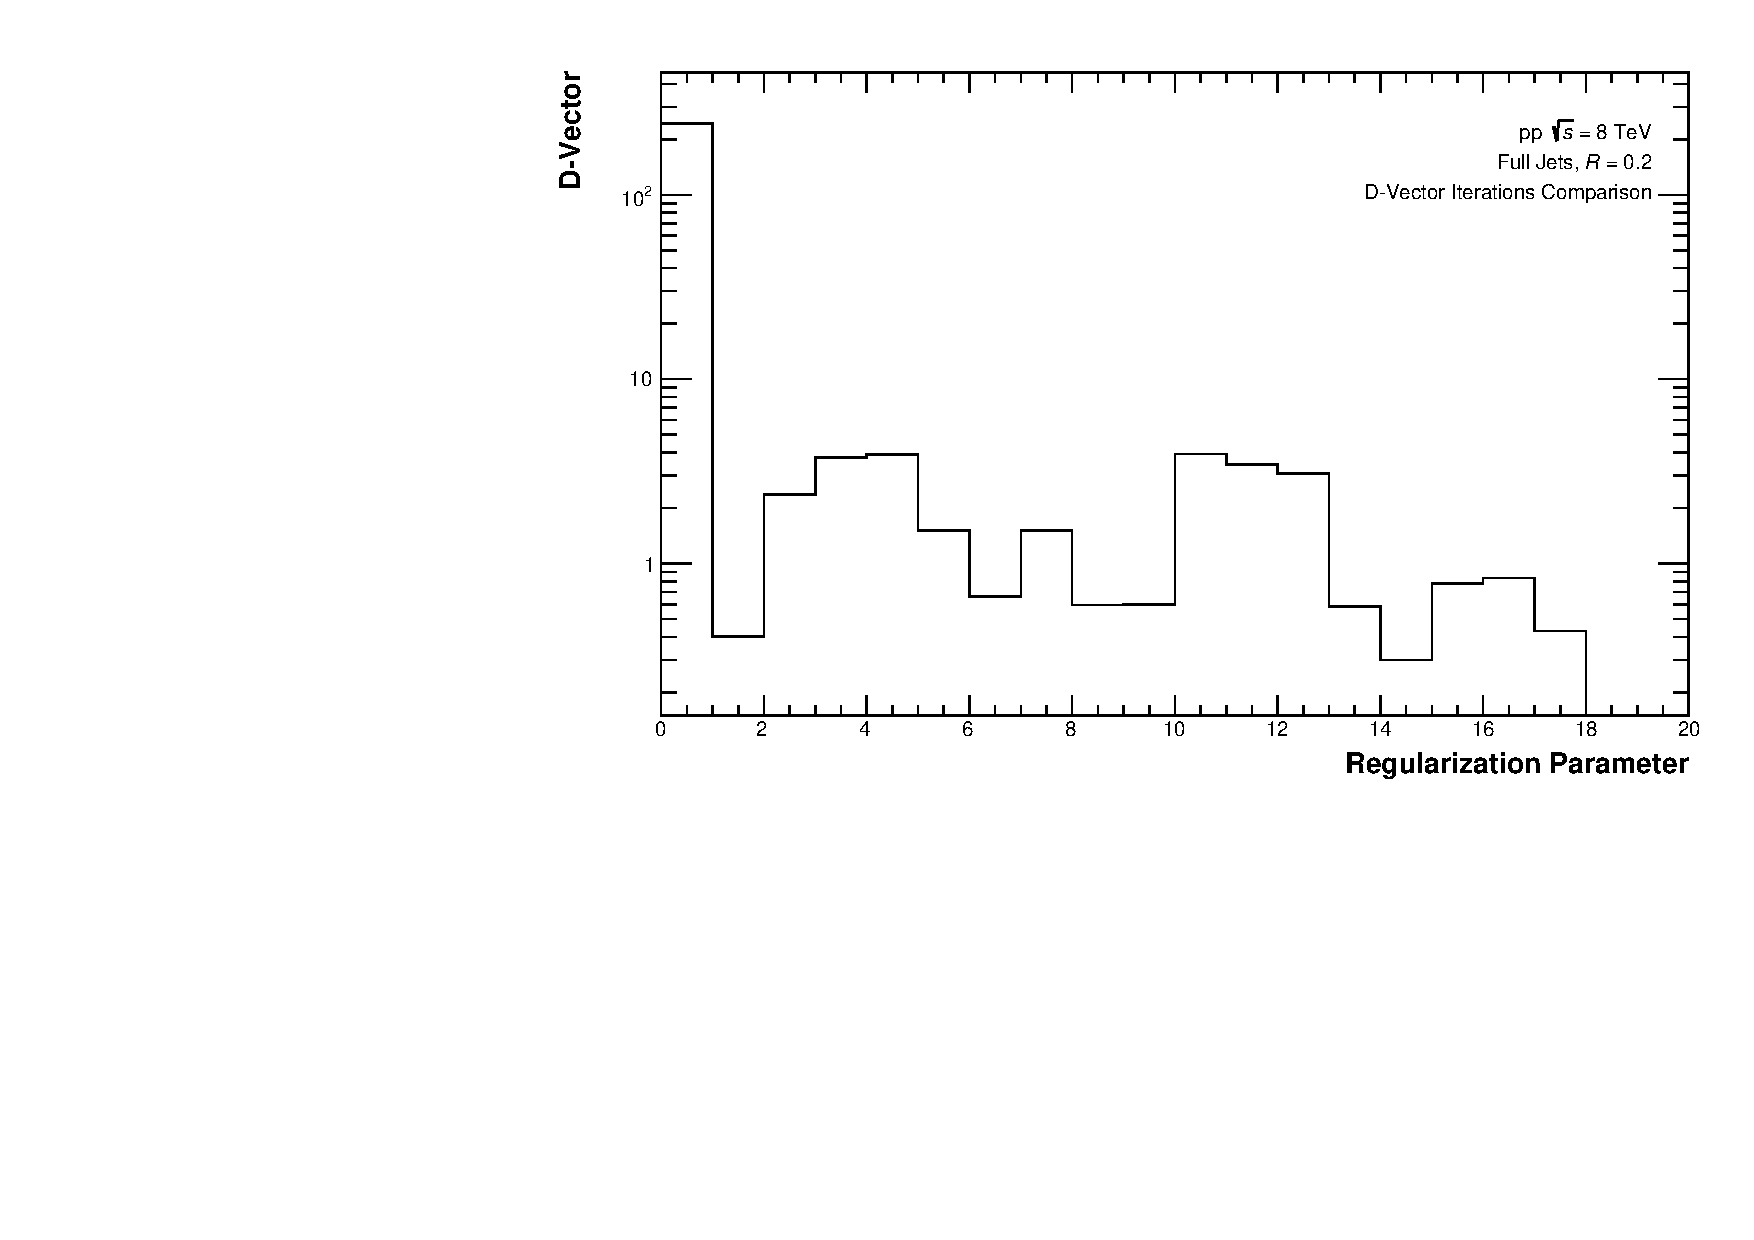
\includegraphics[width=15cm]{figures/DVector/DVector_R02.pdf}
    \caption{D-Vector comparison for different iterations.}
    \label{fig:DVector}
\end{figure}

\begin{figure}
    \centering
    \begin{multicols}{2}
        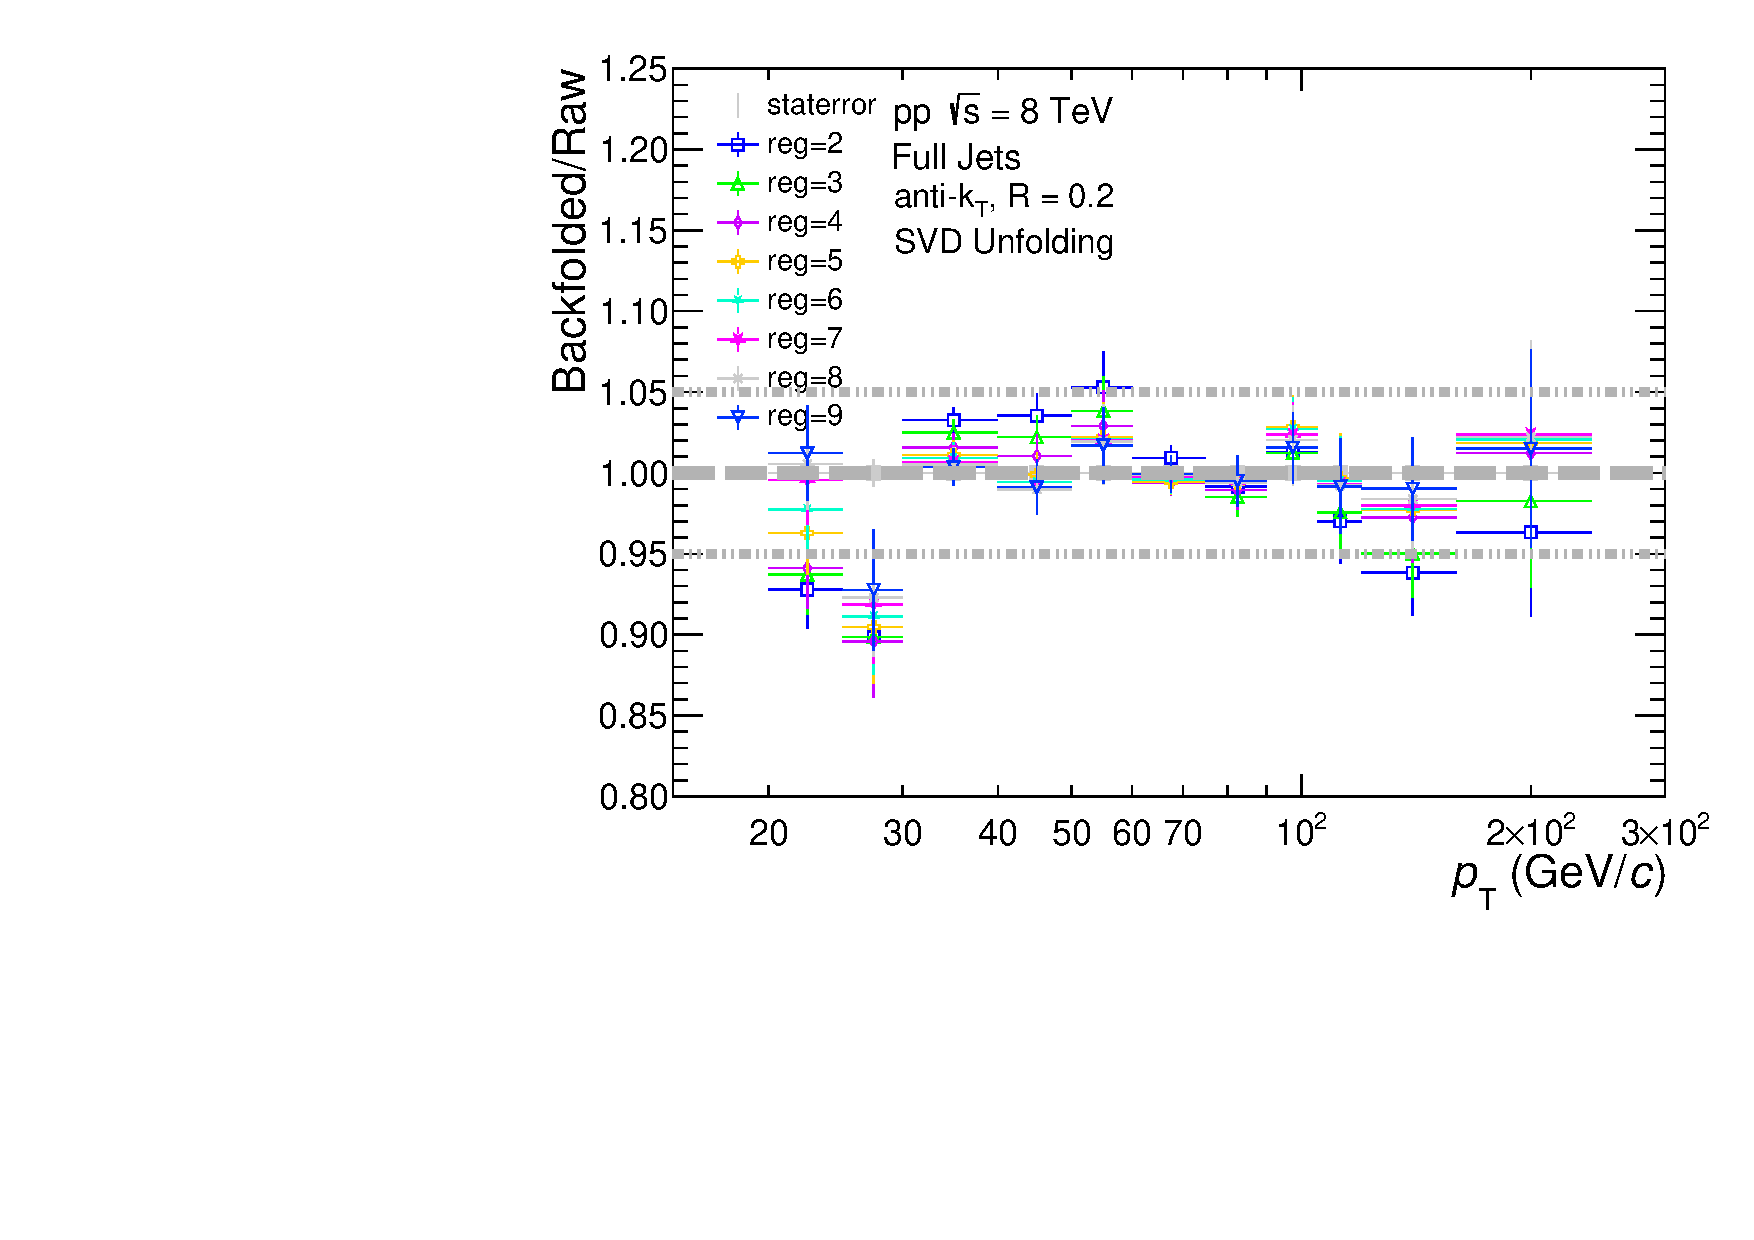
\includegraphics[width=7.5cm]{figures/UnfoldingComparisons/BackfoldedVsRaw/RatioFoldRawSvd_R02.pdf}
    \vfill\null
    \columnbreak
        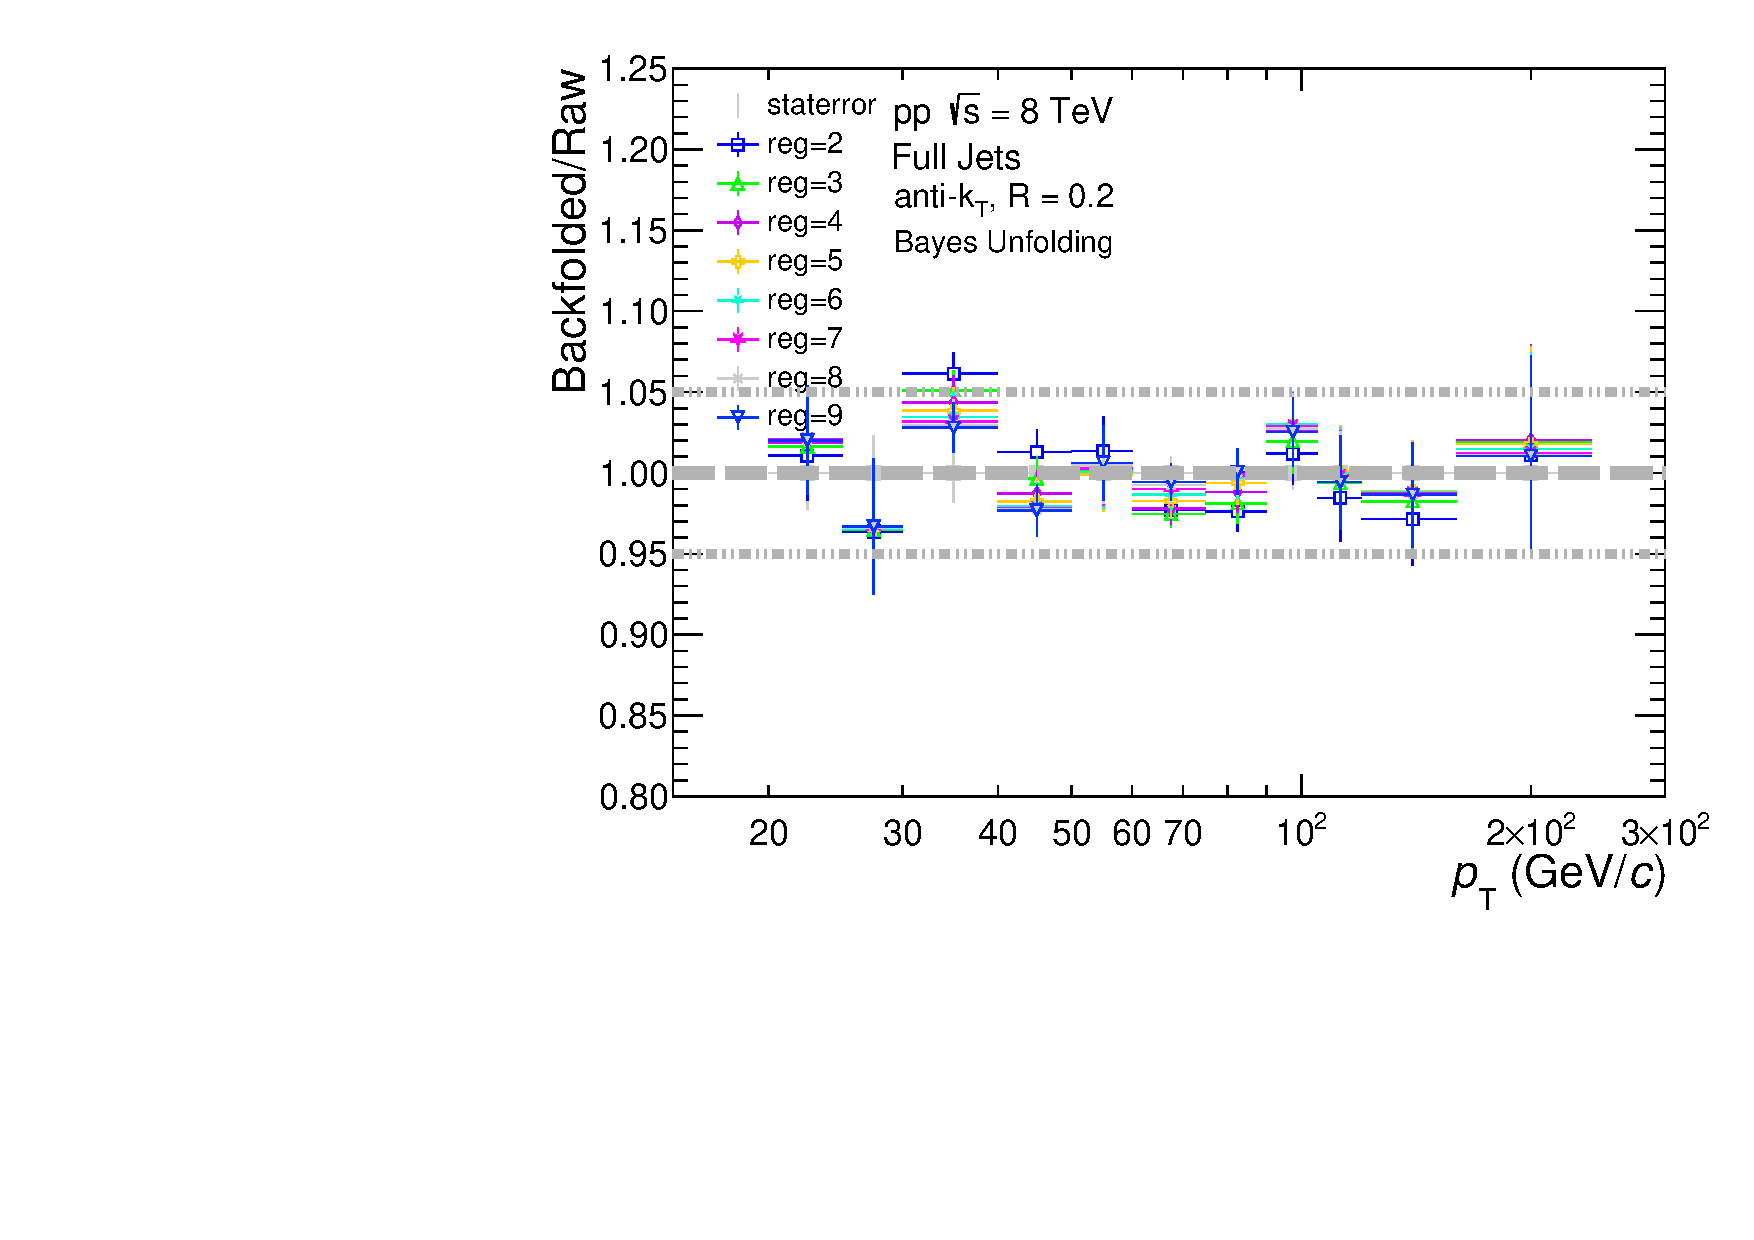
\includegraphics[width=7.5cm]{figures/UnfoldingComparisons/BackfoldedVsRaw/RatioFoldRawBayes_R02.pdf}
        \vfill\null
    \end{multicols}
    \caption{Backfolded vs. Raw for R=0.2.}
    \label{fig:BackfoldedRaw}
\end{figure}

Fig. \ref{fig:BackfoldedRaw} shows the comparison of the back-folded spectrum to the raw spectrum for several regularizations for SVD and bayesian unfolding. Using the default settings for regularization and number of iterations the two unfolding methods produce consistent results. For the largest jet radius some oscillating behavior can be seen. The difference between the unfolding methods is accounted for as systematic uncertainty.

\begin{figure}
    \centering
    \begin{multicols}{2}
            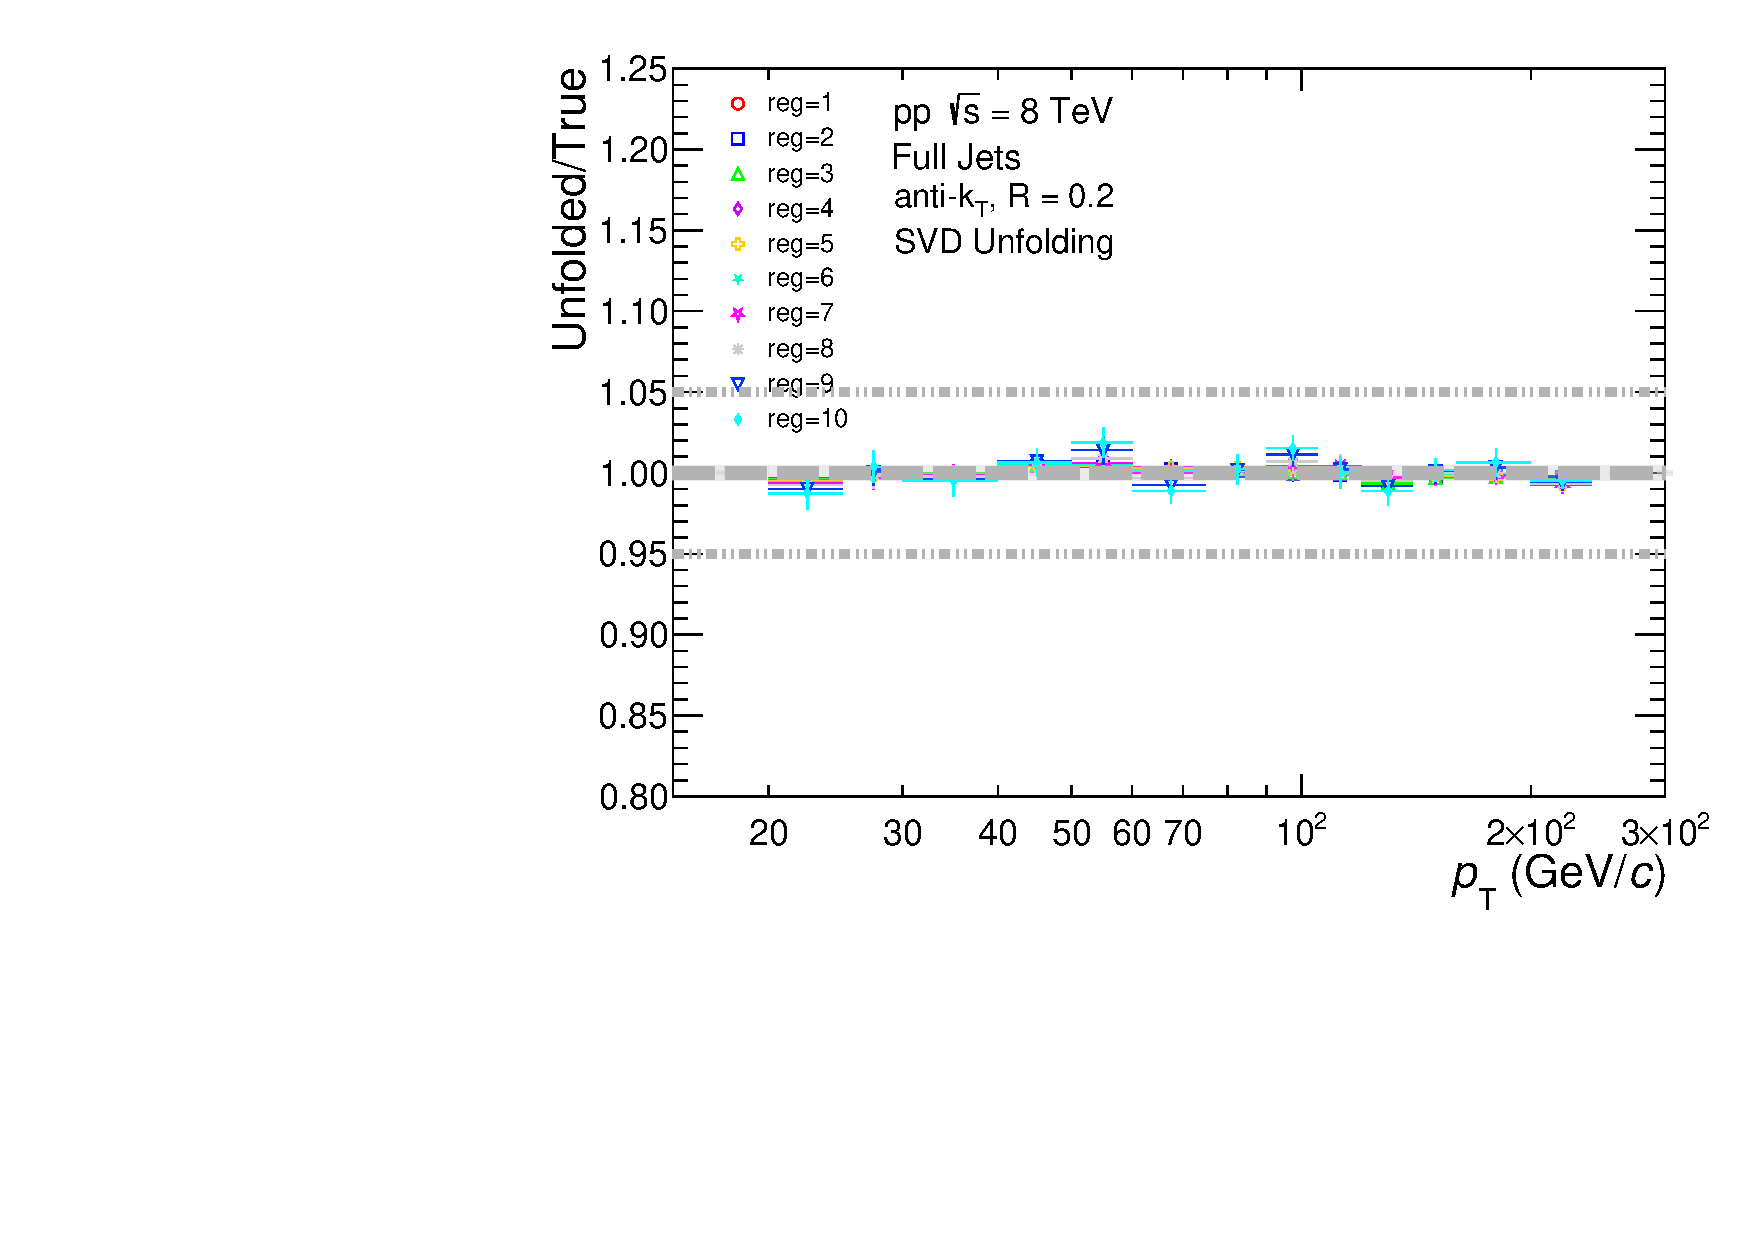
\includegraphics[width=7.5cm]{figures/UnfoldingComparisons/Closure/RatioClosure1DSvd_R02.pdf}
        \vfill\null
        \columnbreak
            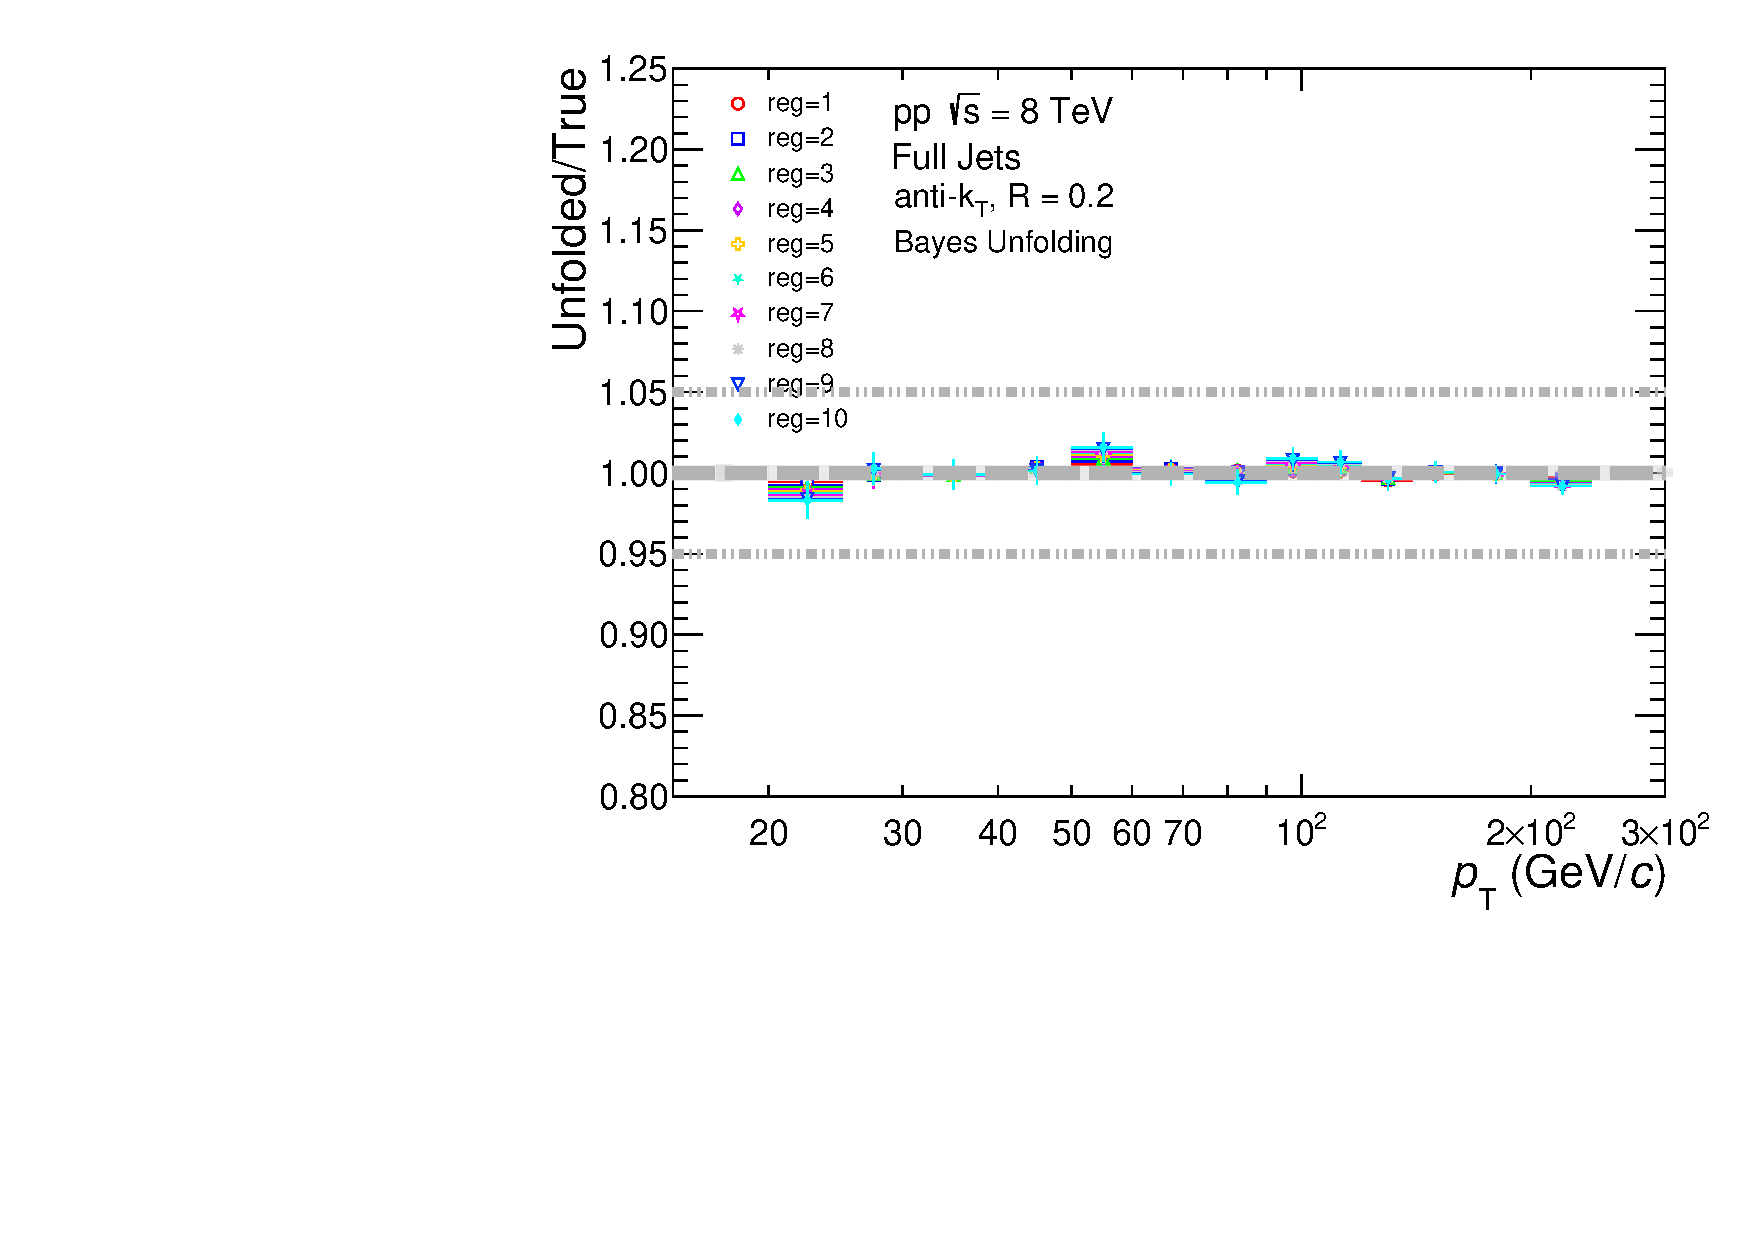
\includegraphics[width=7.5cm]{figures/UnfoldingComparisons/Closure/RatioClosure1DBayes_R02.pdf}
        \vfill\null
    \end{multicols}
    \caption{Closure test for R=0.2.}
    \label{fig:Closure}
\end{figure}

Fig. \ref{fig:Closure} shows the MC closure test for SVD and bayesian unfolding, where the MC sample is split randomly, with 20$\%$ used for the smeared spectrum, and 80$\%$ used for the response matrix. Good agreement between the true spectrum and the unfolded solution is found.

\DIFaddbegin \subsubsection{\DIFadd{Unfolding tests - }\pPb}

\DIFadd{\textcolor{red}{Duplicate the unfolding test section with \pPb plots.}
}

\DIFaddend \subsection{Study of a bias the spectrum at high-\texorpdfstring{\pT}{pT} due to possible fake contributions}
\label{sec:biasStudy}

The track sample at high-\pT is contaminated by fake tracks, originating either from a misreconstruction of the \pT of tracks with lower momenta, or from a contamination of tracks from muons from cosmic or atmospheric sources passing the detector in coincidence with triggered events. A study was done to account for these fake tracks and can be found in \cite{anaNoteMFasel}.\clearpage{}
\clearpage{}\DIFaddbegin \section{\DIFadd{Nuclear modification factor}}
\label{sec:nuclearModFac}

\DIFadd{\textcolor{red}{Section on building the RpA.}}\clearpage{}
\clearpage{}\DIFaddend \section{Systematic Uncertainties}
\label{chap:Systematics}

\subsection{Spectra}
\label{sec:SystematicsSpectra}

Below are the studied sources of systematic uncertainty and their details. For each of the systematics, the analysis was repeated from start to finish for each variation and required either a seperate subwagon or train run. All variations for one systematic contribution are evaluated simultaneously. The five unfolding systematics are also evaluated together. For each bin in each systematic other than unfolding, the mean of the absolute deviations of all variations is found. For unfolding, the maximum of the absolute deviations of all variations is found. In order to suppress unphysical statistical fluctiations, for most contributions, the mean for all bins is then fit with a 0th - 2nd order polynomial. Some contributions remain as binwise, where the binwise uncertainty is not expected to follow a clear pattern. All the uncertainties are then added in quadrature for each bin.

\begin{itemize}
    \item Tracking efficiency: Variations of $\pm 4\%$ are considered.

    \item Unfolding
    \begin{itemize}
        \item Regularization: The default number of iterations is 6, and variations of +3/-2 iteration are considered.
        \item Truncation: The raw distribution and the response matrix are truncated at different values. The default minimum accepted jet \pT is 10 GeV. As variations, $\pm 5$ GeV are considered.
        \item Prior: The default prior is Pythia 8, the MC used in the generation of the response. The ratio between the default unfolded solution and the default prior is considered. This ratio is applied as a weight to the response prior to unfolding.
        \item Binning: Four bin variations to the measured input are considered. For a list of the binning, see appendix \ref{sec:appendixSysBinVar}.
        \item Unfolding method: Bayesian is used by default with SVD as a variation. The difference between the bayesian and the SVD method is primarily used in order to account for the discrepancy seen between the two methods in the region where the triggers swap.
    \end{itemize}

    \item EMCAL seed thresholds:
    \begin{itemize}
        \item Default: Seed threshold = 300 MeV, cell threshold = 100 MeV
        \item Low: Seed threshold = 275 MeV, cell threshold = 75 MeV
        \item High: Seed threshold = 350 MeV, cell threshold = 100 MeV
    \end{itemize}

    \item Clusterizer algorithm: The default clusterizer algorithm is Clusterizer v3. NxN clusterizer with N = 3 and N = 5 are also considered, where N is the number of EMCal towers.

    \item Hadronic correction: The cluster energy is corrected for the hadronic contribution. By default, the energy of the full track in the ITS-TPC is subtracted from the cluster under assumption of the electron mass (F=1). Two variations are considered. In one case, 70\% of the energy of the matched tracks is subtracted. In the other, the minimally ionizing particle (MIP) energy is subtracted.

    \item Trigger rejection factor fit: The trigger rejection factor is calculated by linearly fitting to the ratio of triggers at the turn-on after corrections for the cluster trigger efficiency. By default, this fit starts at 4 (12.25) GeV for the lower (upper) trigger. Variations of $\pm 0.5 GeV$ are considered. To account for the uncertainty on the rejection factor, these uncertainties are added to the rejection factor fit uncertainty before analysis and adding to the total.

    \item Trigger swap momentum: A momentum must be selected at which to switch from using one trigger to the next higher threshold trigger when combining the spectra. By default, these momenta are 30 and 60 GeV for the EMC7 and EJE triggers, respectively. Variations of $\pm 5 GeV$ are considered for the low trigger swap, while variations of $\pm 10 GeV$ are considered for the high trigger swap.

    \item Maximum track \pT: The analysis puts an upper limit on the track momentum of 200 GeV by default. As variations, 125, 150, 175, and 225 GeV are tested.

    \item Maximum track/cluster energy: The analysis puts an upper limit on the cluster energy of 200 GeV by default. The same variation used for the track momentum are tested.

    \item Q/\pT Shift: The spectrum is varied for the Q/\pT shift caused by space-time distortions in the TPC. By default, no shift is considered. The variation considered is 2e-3. This shift was determined by running a PYTHIA 8 simulation and applying a shift to the tracks. The shift that matches the shift in data the closest is chosen. See figure \ref{fig:QoverPtShift}
\end{itemize}

\begin{figure}
    \centering
    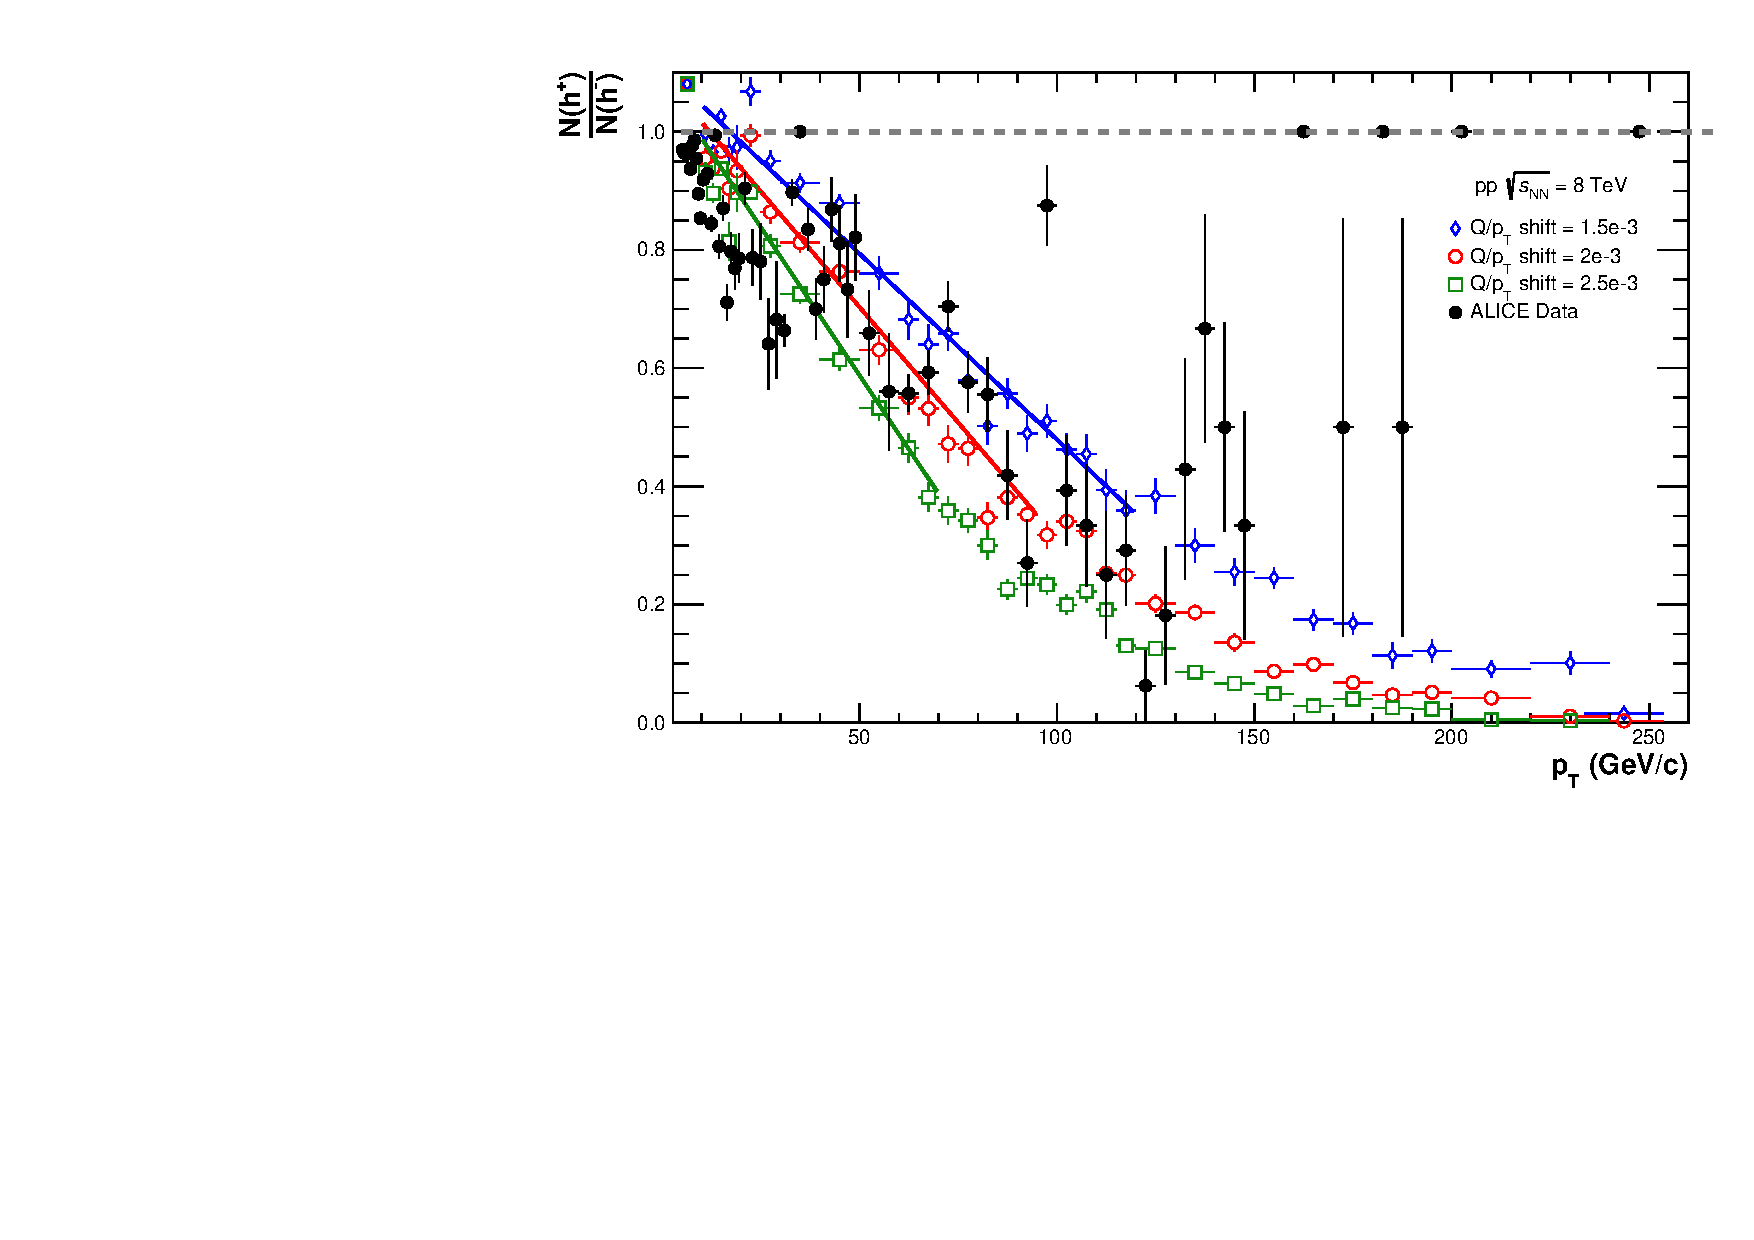
\includegraphics[width=15cm]{figures/QoverPtShift/QPTComparison.pdf}
    \caption{Comparison of different Q/\pT shift values.}
    \label{fig:QoverPtShift}
\end{figure}

\DIFaddbegin \DIFadd{Some additional uncertainties are required for }\pPb\DIFadd{. These are as follows:
}

\begin{itemize}
    \item \DIFadd{\textcolor{red}{BG sub uncertainty}
    }\item \DIFadd{\textcolor{red}{Any uncertainties from embedding? Probably.}
    }\item \DIFadd{\textcolor{red}{I also assumed there's something from 8 vs. 8.16 TeV discrepancy.}
}\end{itemize}

\DIFaddend The components of the uncertainty are then added in quadrature. The different components of the systematic uncertainties for R = 0.2 jets are shown in Fig. \ref{fig:SystematicsSpectraR02} (for other jet radii and individual contributions, see appendix \ref{sec:AppendixSystematics}).

\begin{figure}
    \centering
    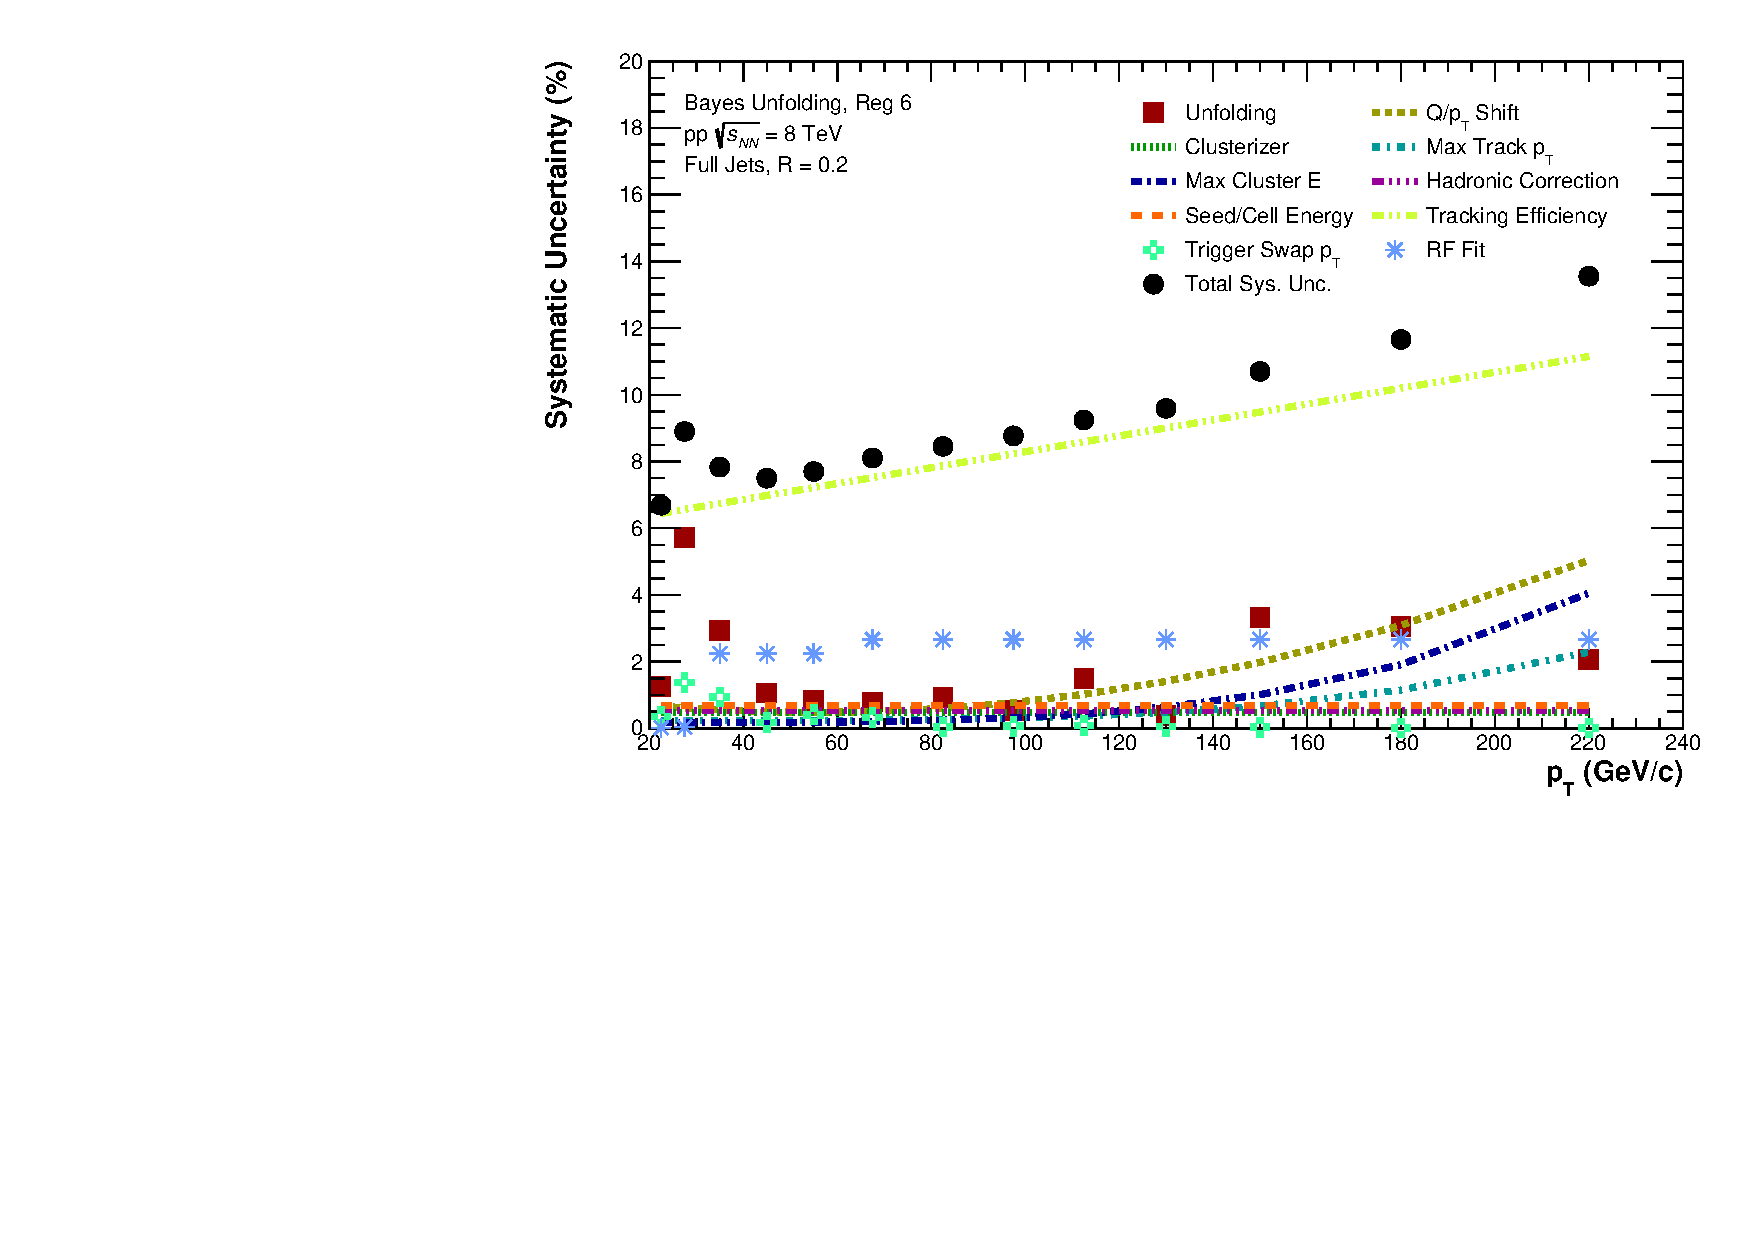
\includegraphics[width=15cm]{figures/Systematics/TotalSystematics_R02.pdf}
    \caption{All sources of systematic uncertainties, including the total systematic uncertainty with all components added in quadrature \DIFaddbeginFL \DIFaddFL{for }\pp \DIFaddFL{(left) and }\pPb \DIFaddFL{(right) \textcolor{red}{insert \pPb plot}}\DIFaddendFL .}
    \label{fig:SystematicsSpectraR02}
\end{figure}

\subsection{Cross-Section Ratios}
\label{sec:SystematicsRatios}

For the cross-section ratios, the same systematic contributions are considered. With the exception of the trigger rejection factor fit, trigger swap, and unfolding systematics, all contributions are calculated directly on the ratio, resulting in partial cancelling \DIFaddbegin \DIFadd{\textcolor{red}{see what is required for \pPb. Some stuff might/might not cancel, etc}}\DIFaddend . The rejection factor fit is not included at all, since this contribution cancels entirely. The trigger swap and unfolding contributions for each cross-section in the ratio are added in quadrature to the total uncertainty. The different components of the systematic uncertainties for R = 0.2/0.3 jets are shown in Fig. \ref{fig:SystematicsRatiosR02} (for other jet radii and individual contributions, see appendix \ref{sec:AppendixSystematics}).

\begin{figure}
    \centering
    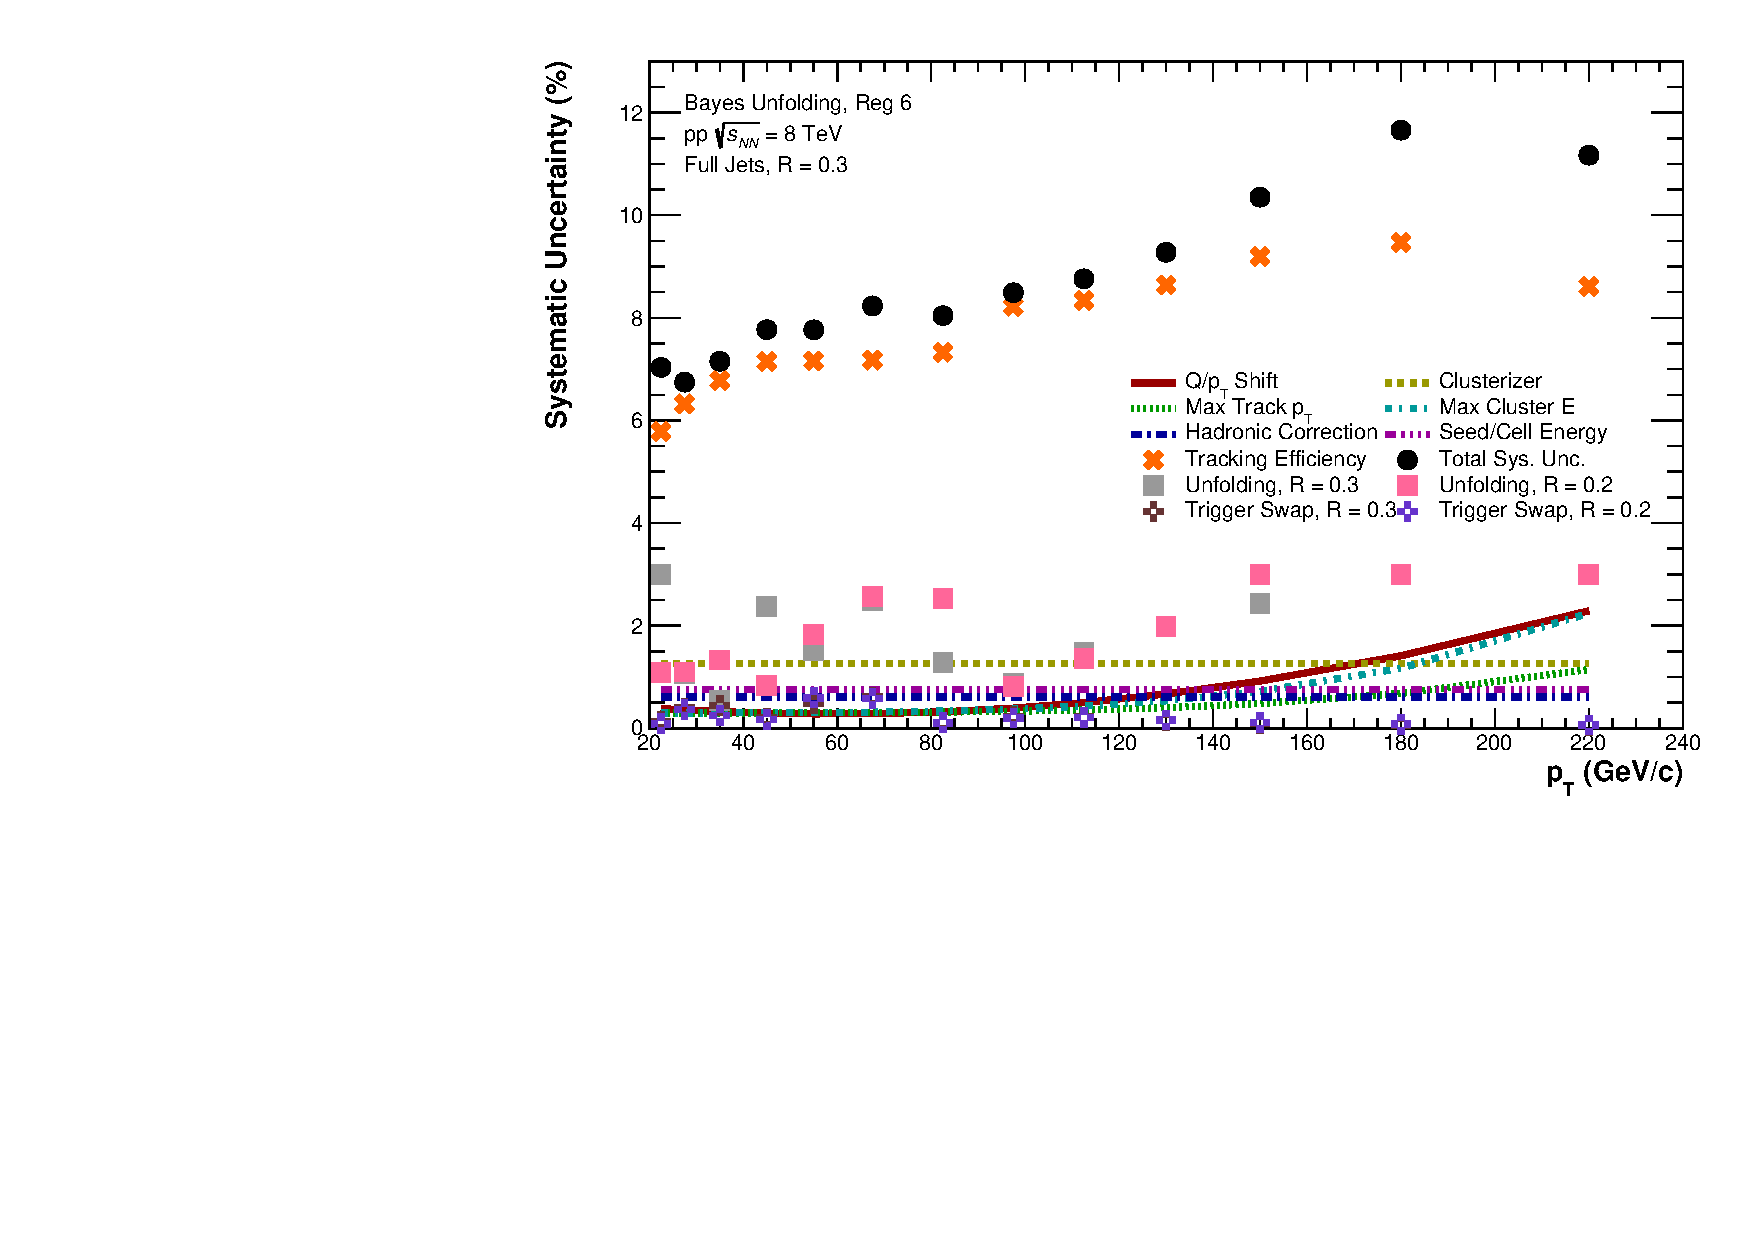
\includegraphics[width=15cm]{figures/Systematics/ratios/TotalSystematics_R02R03.pdf}
    \caption{All sources of systematic uncertainties, including the total systematic uncertainty with all components added in quadrature \DIFaddbeginFL \DIFaddFL{for }\pp \DIFaddFL{(left) and }\pPb \DIFaddFL{(right) \textcolor{red}{\pPb plot}}\DIFaddendFL .}
    \label{fig:SystematicsRatiosR02}
\end{figure}
\DIFaddbegin 

\subsection{\DIFadd{Nuclear modification factor}}
\label{sec:systematicsRpA}

\DIFadd{\textcolor{red}{Section on uncertainties for RpA.}}\DIFaddend \clearpage{}
\clearpage{}\section{Results and Comparison to Simulation}
\label{chap:results}

\subsection{Corrected jet spectrum}
\label{sec:corrJetSpectrum}

\begin{figure}
    \centering
    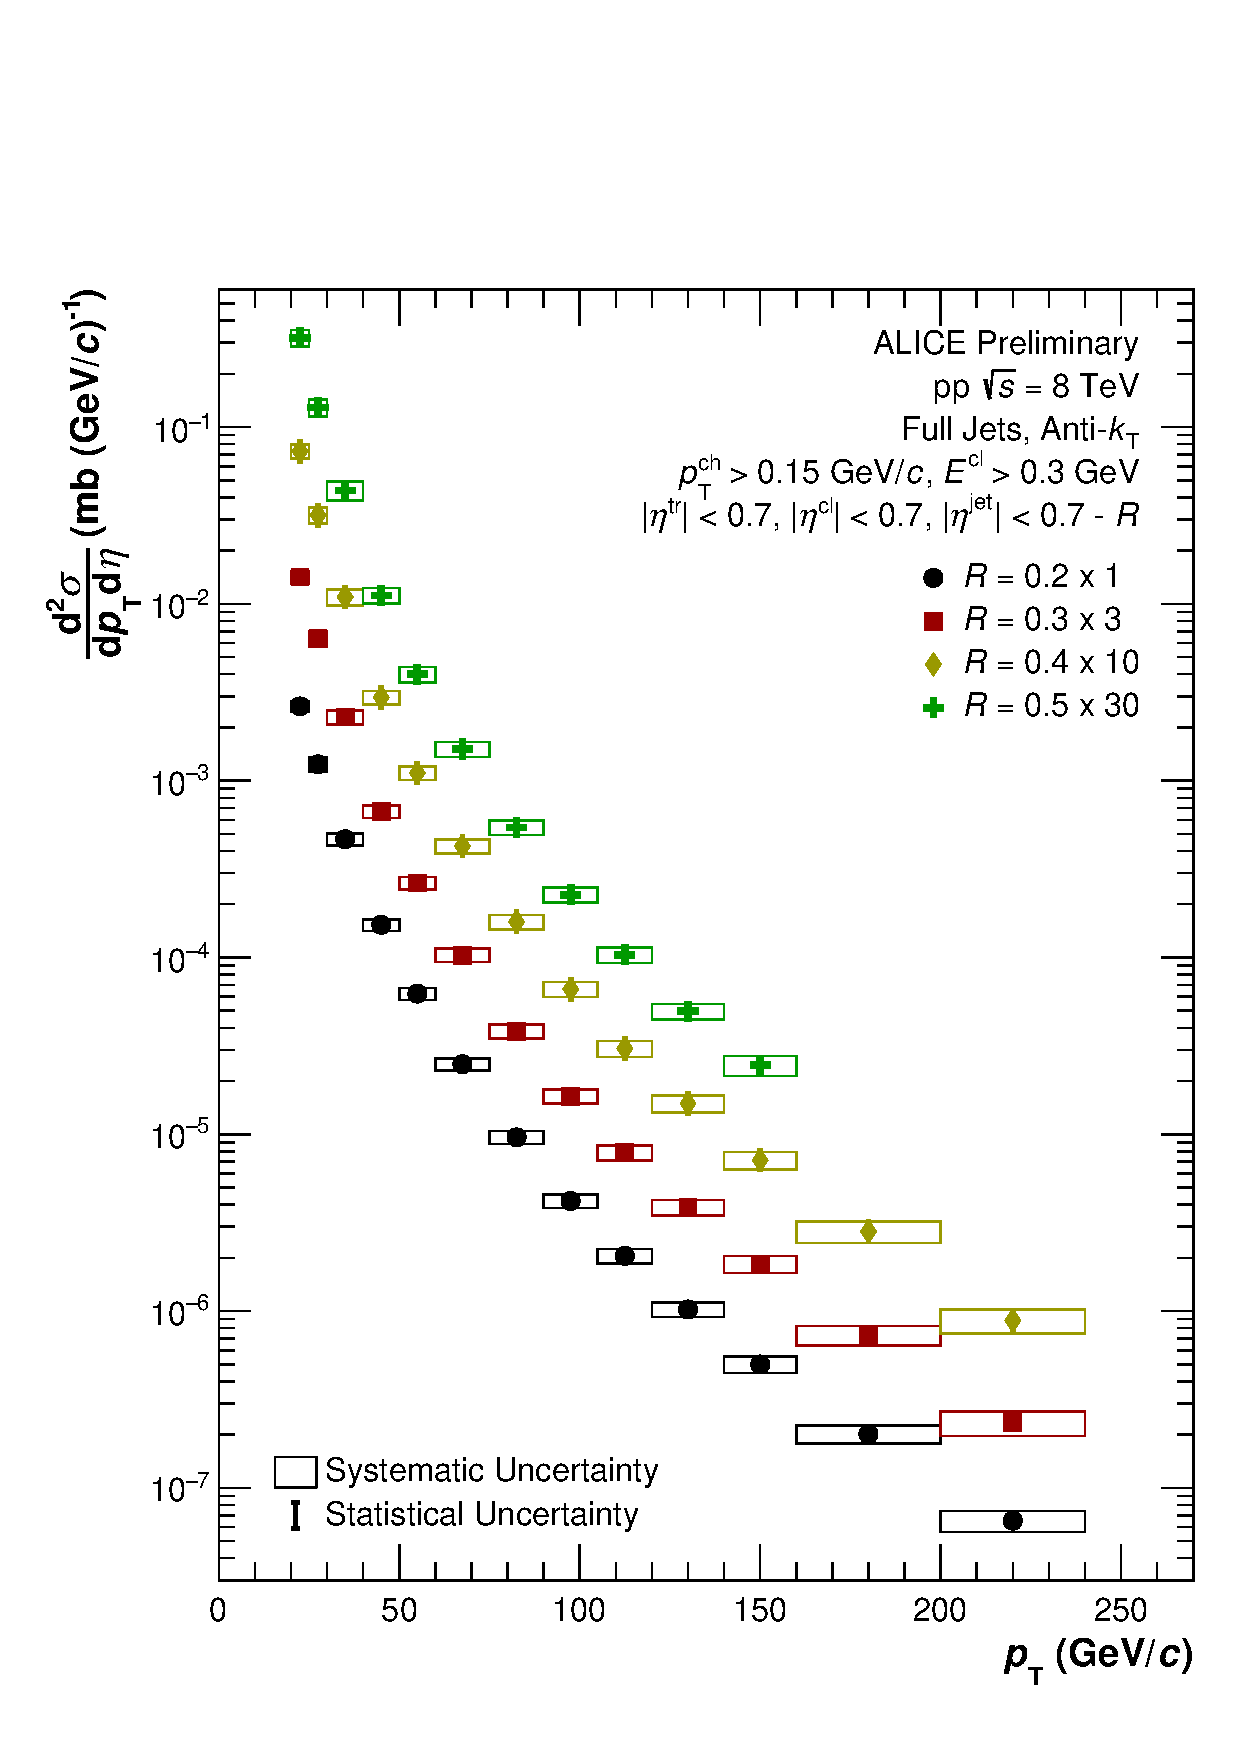
\includegraphics[width=15cm]{figures/FinalResults/Bayes_reg6.pdf}
    \caption{Jet spectra for various jet radii after corrections, unfolding, and addition of systematic errors. Scaled for visual clarity. \DIFaddbeginFL \pp \DIFaddFL{(left) and }\pPb \DIFaddFL{(right) \textcolor{red}{\pPb plot}.}\DIFaddendFL }
    \label{fig:finalSpectra}
\end{figure}

\begin{figure}
    \centering
    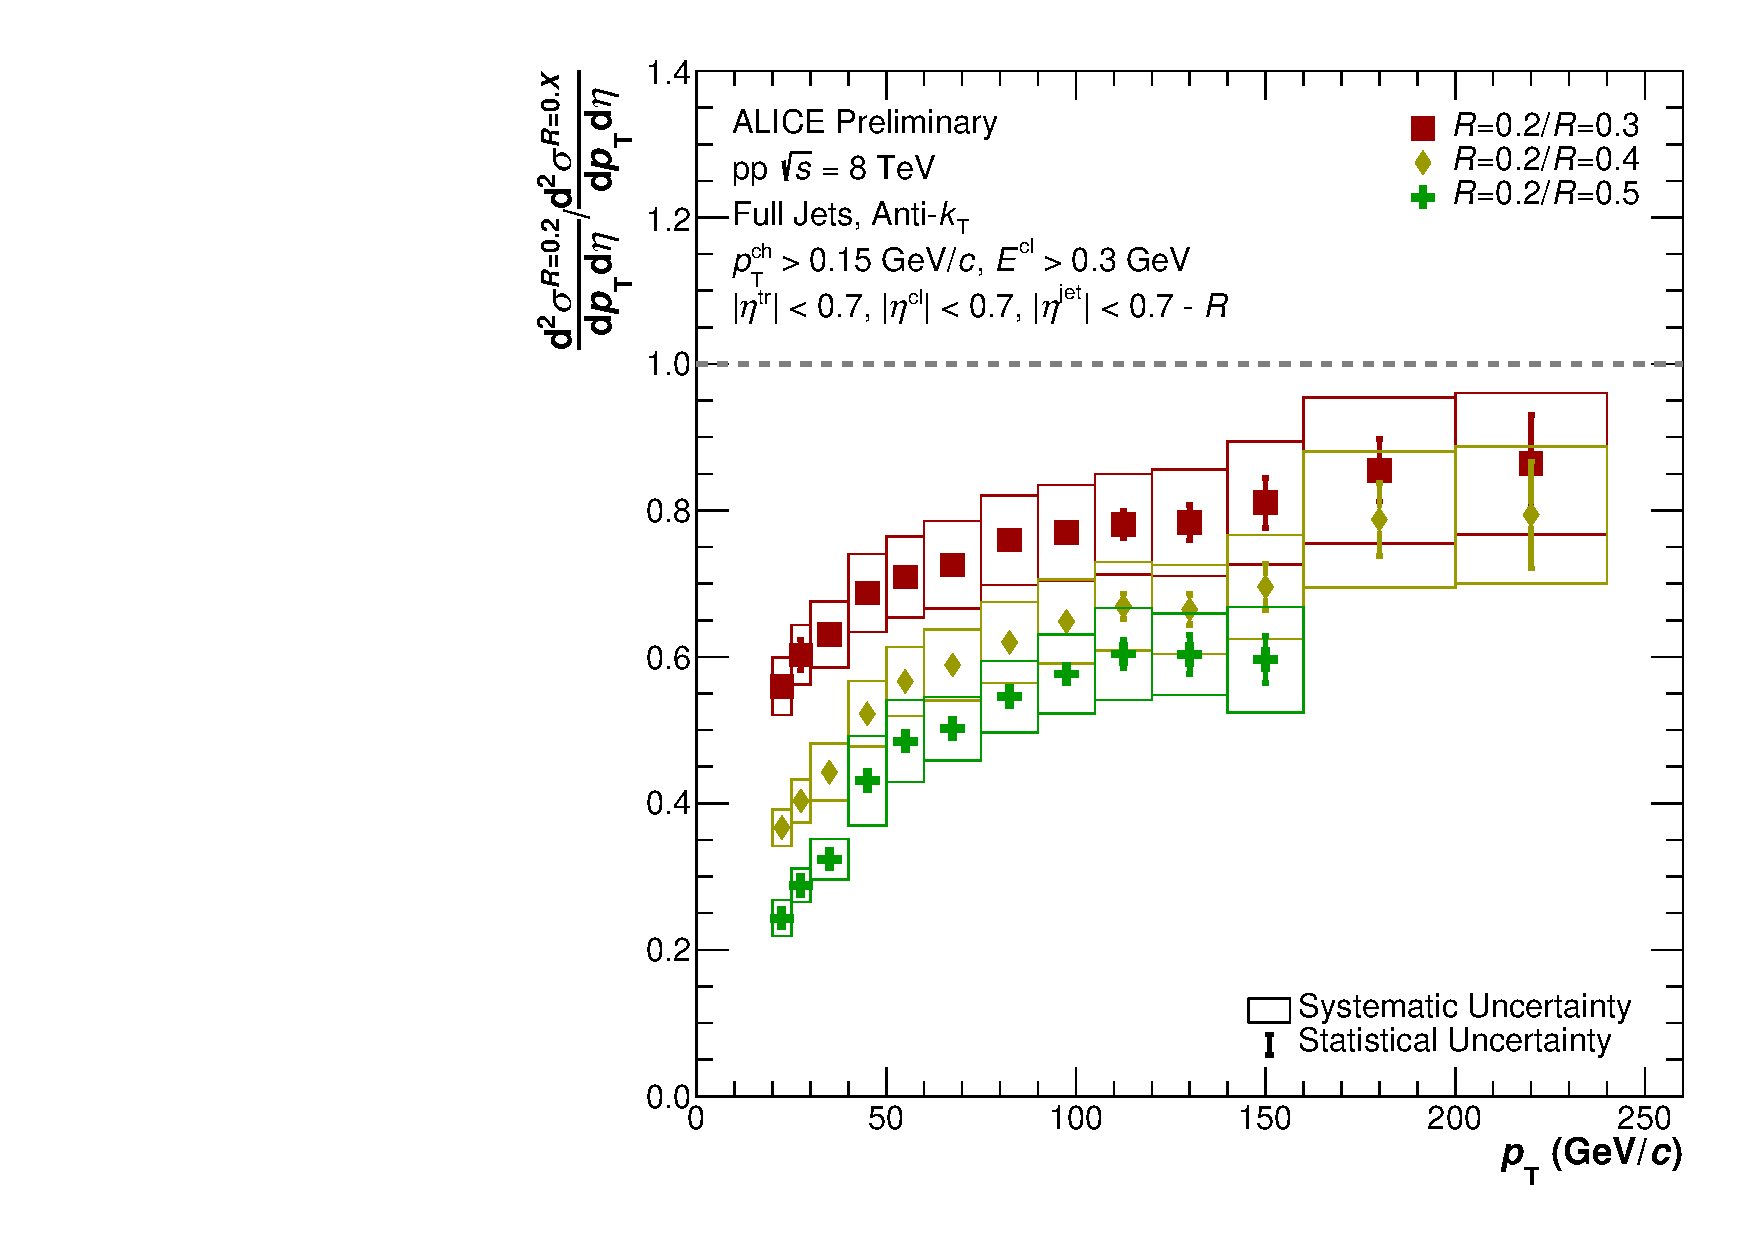
\includegraphics[width=15cm]{figures/FinalResults/Bayes_reg6_Ratio.pdf}
    \caption{Jet spectra for various jet radii compared to R = 0.2 after corrections, unfolding, and addition of systematic errors. \DIFaddbeginFL \pp \DIFaddFL{(left) and }\pPb \DIFaddFL{(right) \textcolor{red}{\pPb plot}.}\DIFaddendFL }
    \label{fig:finalSpectraRatios}
\end{figure}

Fig. \ref{fig:finalSpectra} shows the comparison of the jet \pT spectra for the different jet radii, while fig. \ref{fig:finalSpectraRatios} shows the ratio of R = 0.2 and the remaining radii. Three plotting variations of the final spectra can be found in figures \ref{fig:finalSpectraLogX}, \ref{fig:finalSpectraUnscaled}, and \ref{fig:finalSpectraUnscaledLogX}.
The measurements are shown in the selected \pT regions.

\begin{figure}
    \centering
    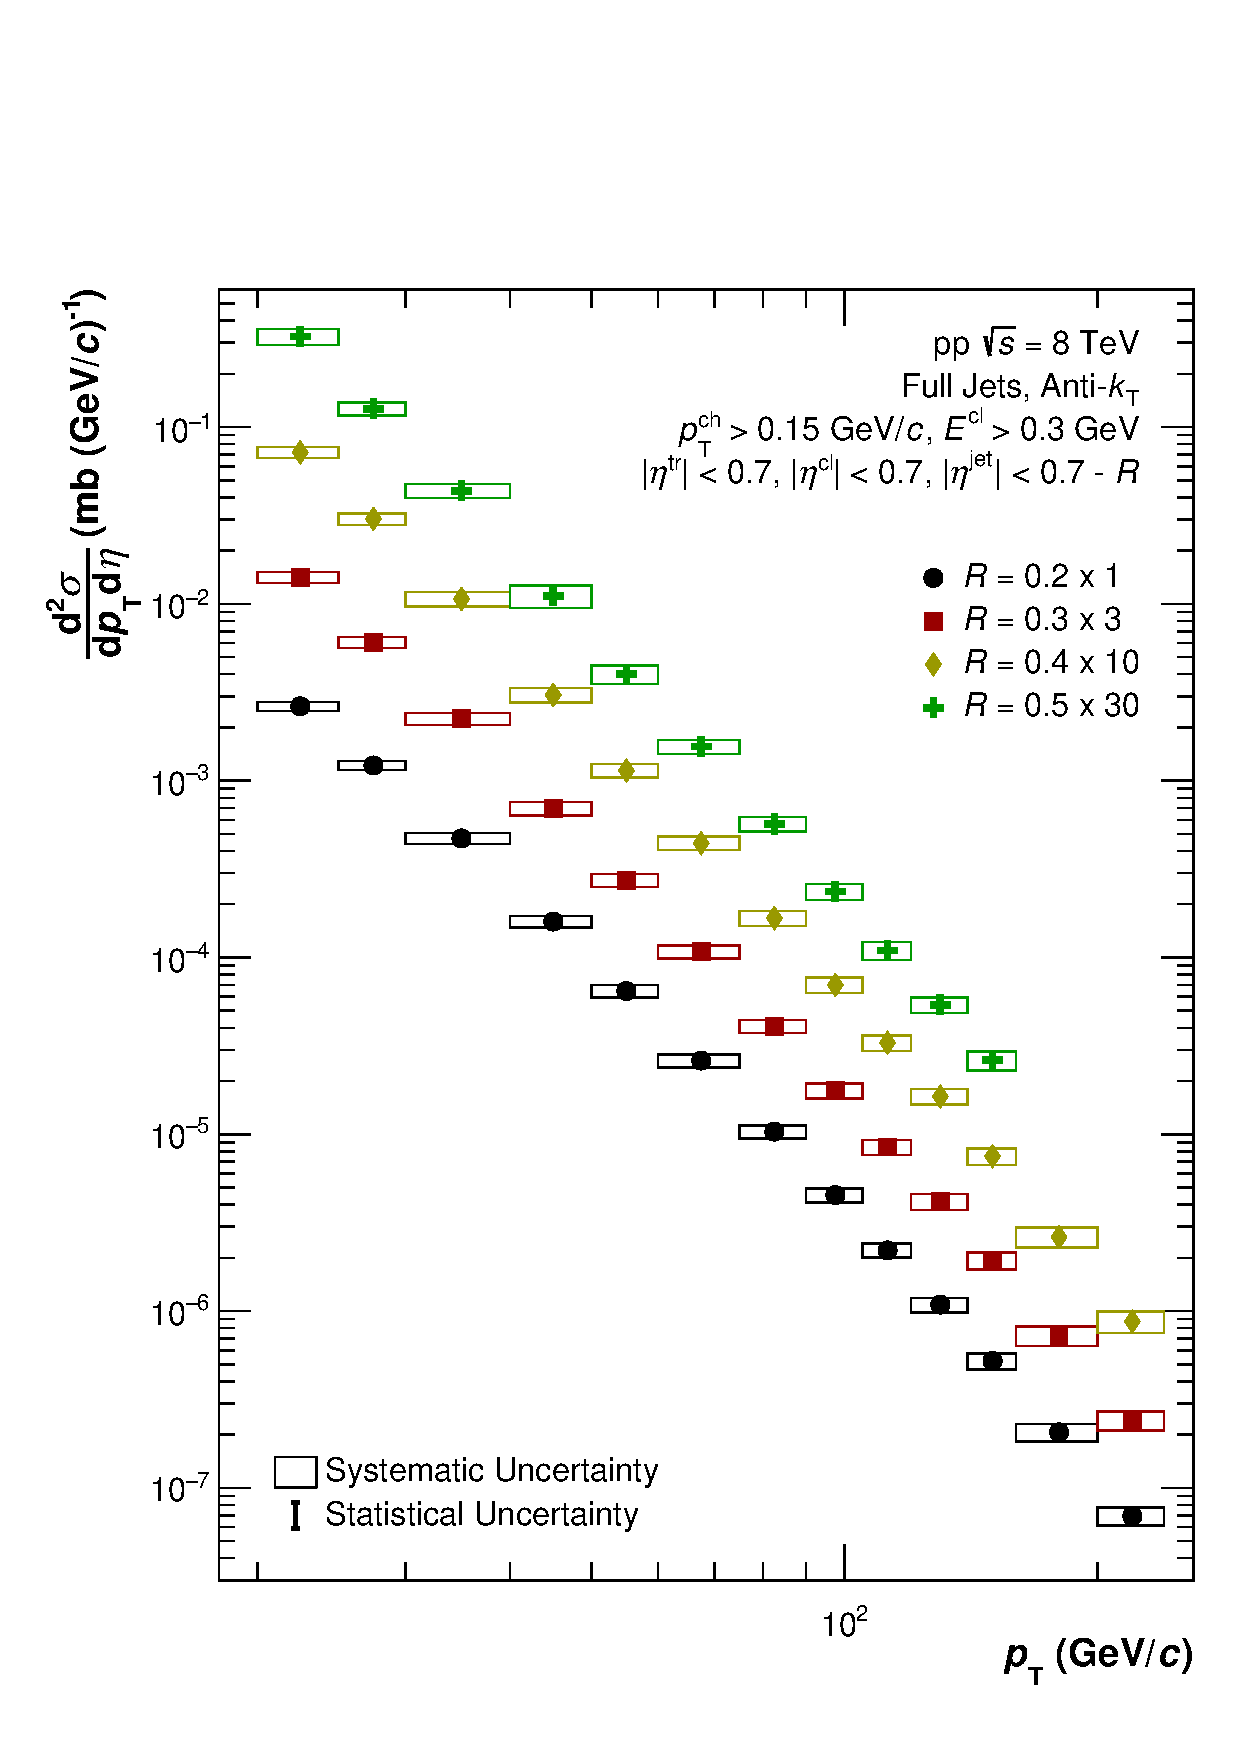
\includegraphics[width=15cm]{figures/FinalResults/Bayes_reg6_logx.pdf}
    \caption{Jet spectra with a logarithmic x-axis for various jet radii after corrections, unfolding, and addition of systematic errors. Scaled for visual clarity. \DIFaddbeginFL \pp \DIFaddFL{(left) and }\pPb \DIFaddFL{(right) \textcolor{red}{\pPb plot}.}\DIFaddendFL }
    \label{fig:finalSpectraLogX}
\end{figure}

\begin{figure}
    \centering
    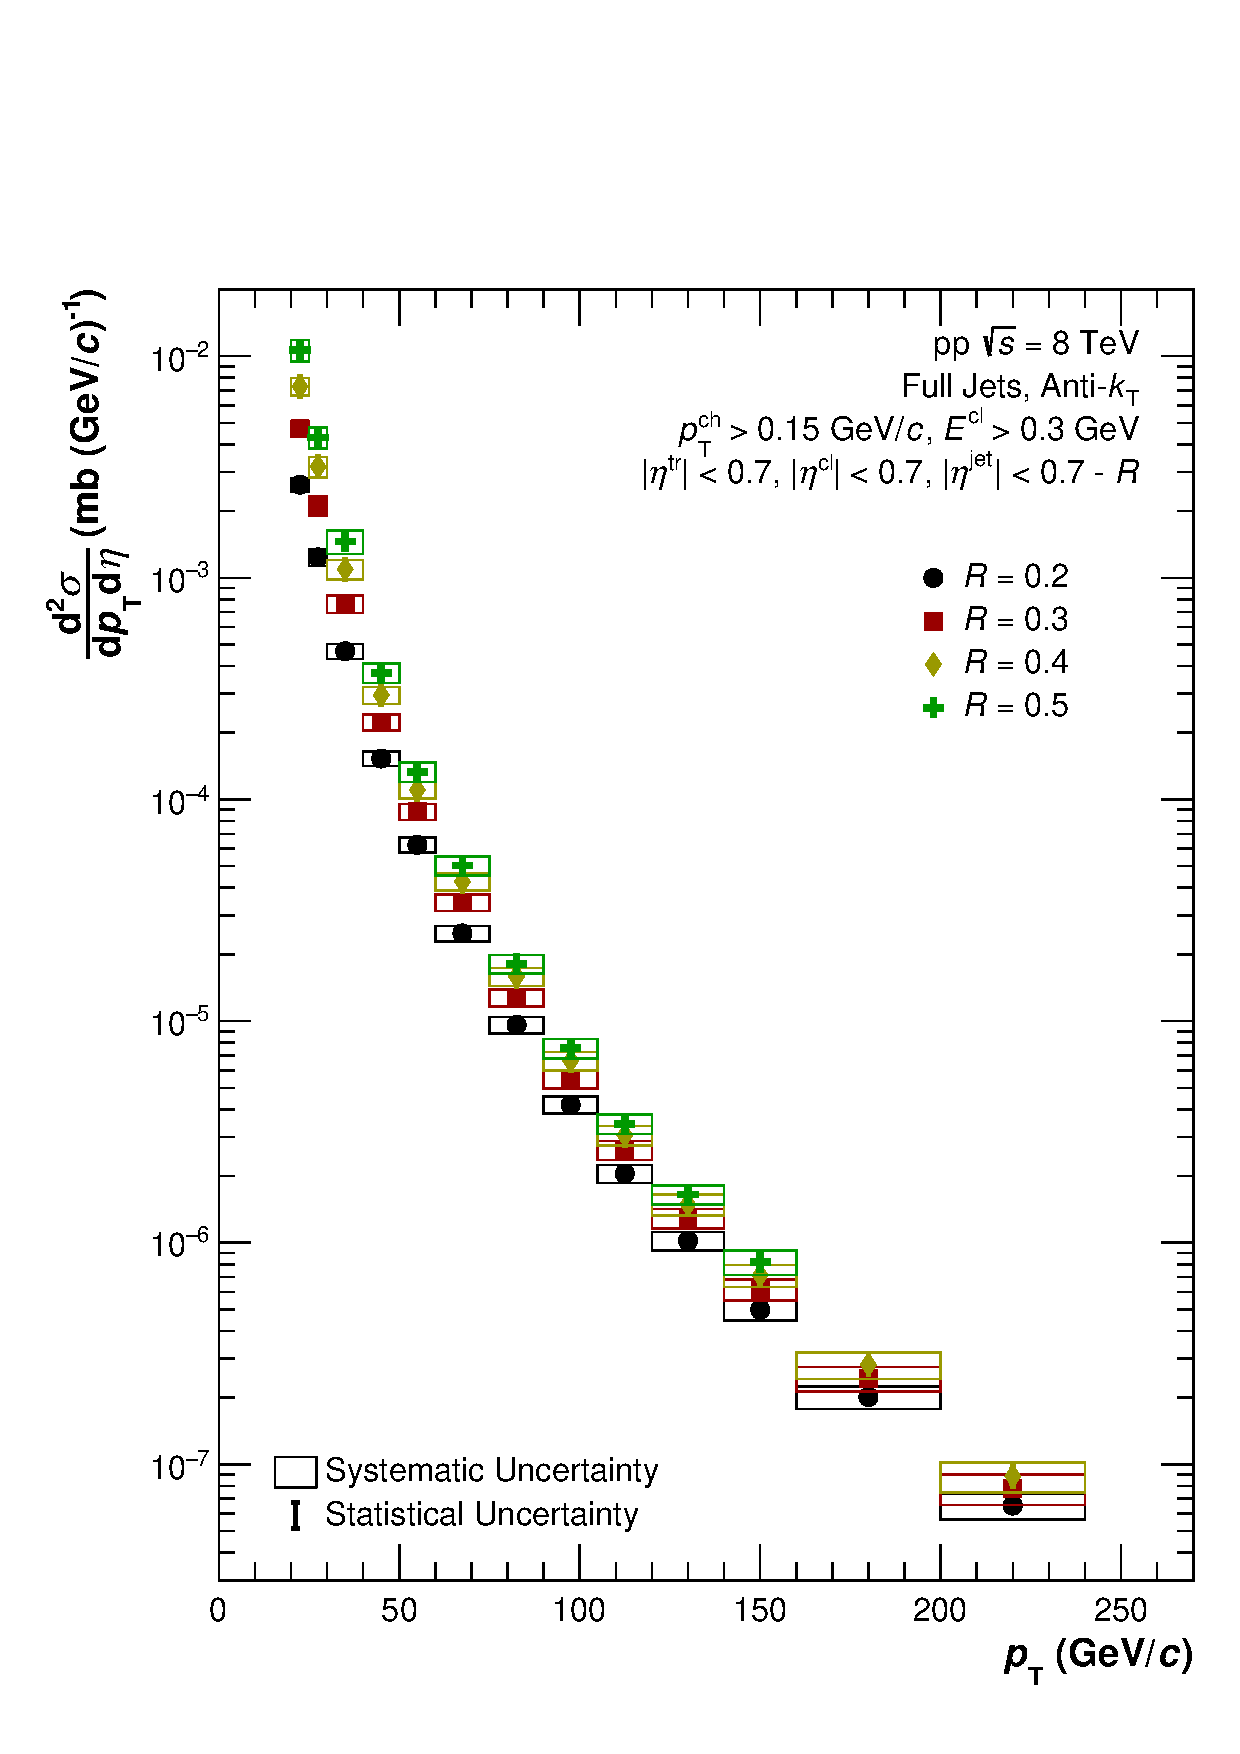
\includegraphics[width=15cm]{figures/FinalResults/Bayes_reg6_unscaled.pdf}
    \caption{Jet spectra for various jet radii after corrections, unfolding, and addition of systematic errors. Unscaled. \DIFaddbeginFL \pp \DIFaddFL{(left) and }\pPb \DIFaddFL{(right) \textcolor{red}{\pPb plot}.}\DIFaddendFL }
    \label{fig:finalSpectraUnscaled}
\end{figure}

\begin{figure}
    \centering
    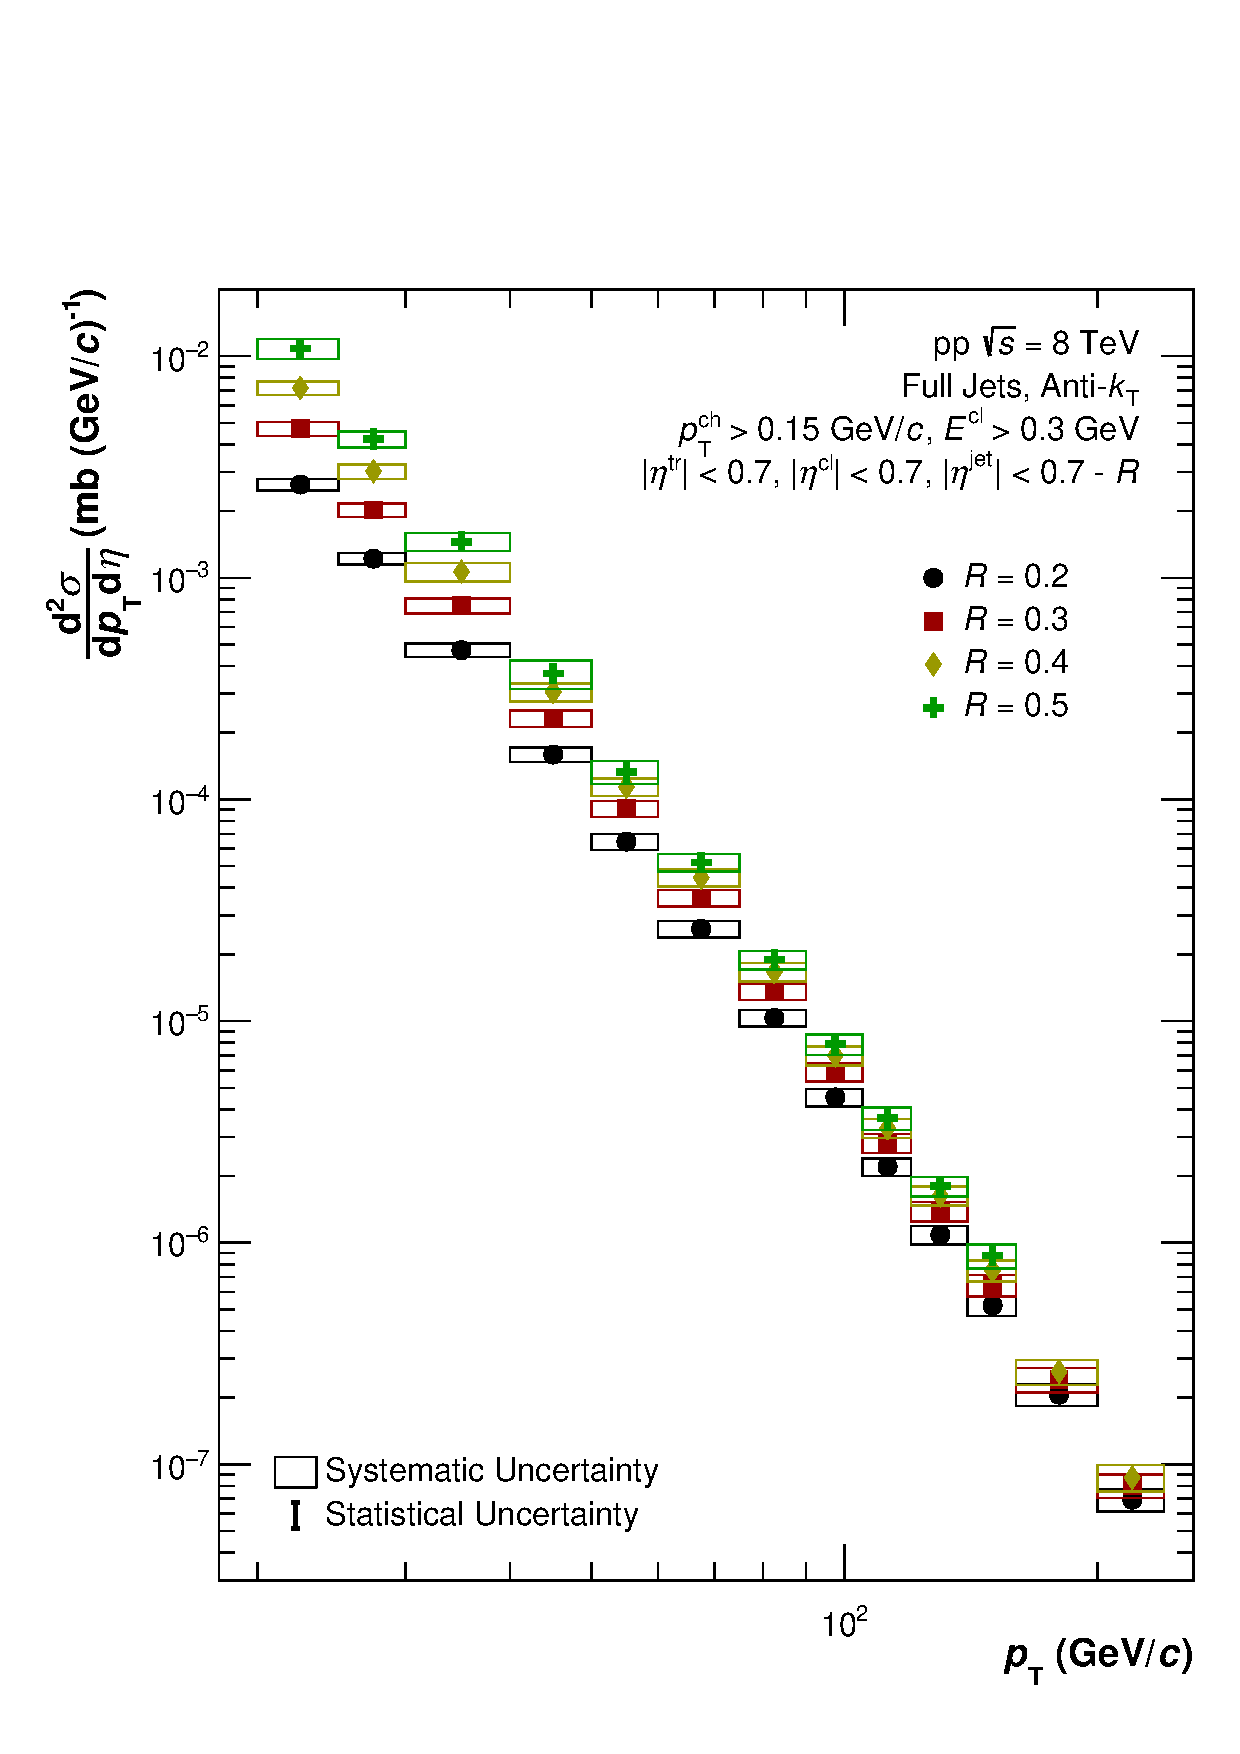
\includegraphics[width=15cm]{figures/FinalResults/Bayes_reg6_logx_unscaled.pdf}
    \caption{Jet spectra with a logarithmic x-axis for various jet radii after corrections, unfolding, and addition of systematic errors. Unscaled. \DIFaddbeginFL \pp \DIFaddFL{(left) and }\pPb \DIFaddFL{(right) \textcolor{red}{\pPb plot}.}\DIFaddendFL }
    \label{fig:finalSpectraUnscaledLogX}
\end{figure}

\DIFaddbegin \subsection{\DIFadd{Nuclear modification factor}}
\label{sec:resultsRpA}

\DIFadd{\textcolor{red}{RpA results}
}

\DIFaddend \subsection{Comparison to PYTHIA8}
\label{sec:mcComparison}

The jet spectra are compared to calculations done in the framework of PYTHIA8.
Fig. \ref{fig:MCGen} shows the comparison of the jet spectra for jet radii R = 0.2 and R = 0.6 to the generator model, and \ref{fig:MCGen_RatioDataMC} shows the ratio of simulation to ALICE data. Fig. \ref{fig:MCGen_Ratio} shows the ratios of radii 0.2/0.3 and 0.2/0.6 compared to the generator model. It is known that PYTHIA overshoots the \DIFaddbegin \pp \DIFaddend data by roughly 40-50\%. It has been seen in all collision systems so far, and can also be observed here. \DIFaddbegin \DIFadd{\textcolor{red}{Do I want these for \pPb?}
}\DIFaddend 

\begin{figure}
    \centering
    \begin{multicols}{2}
            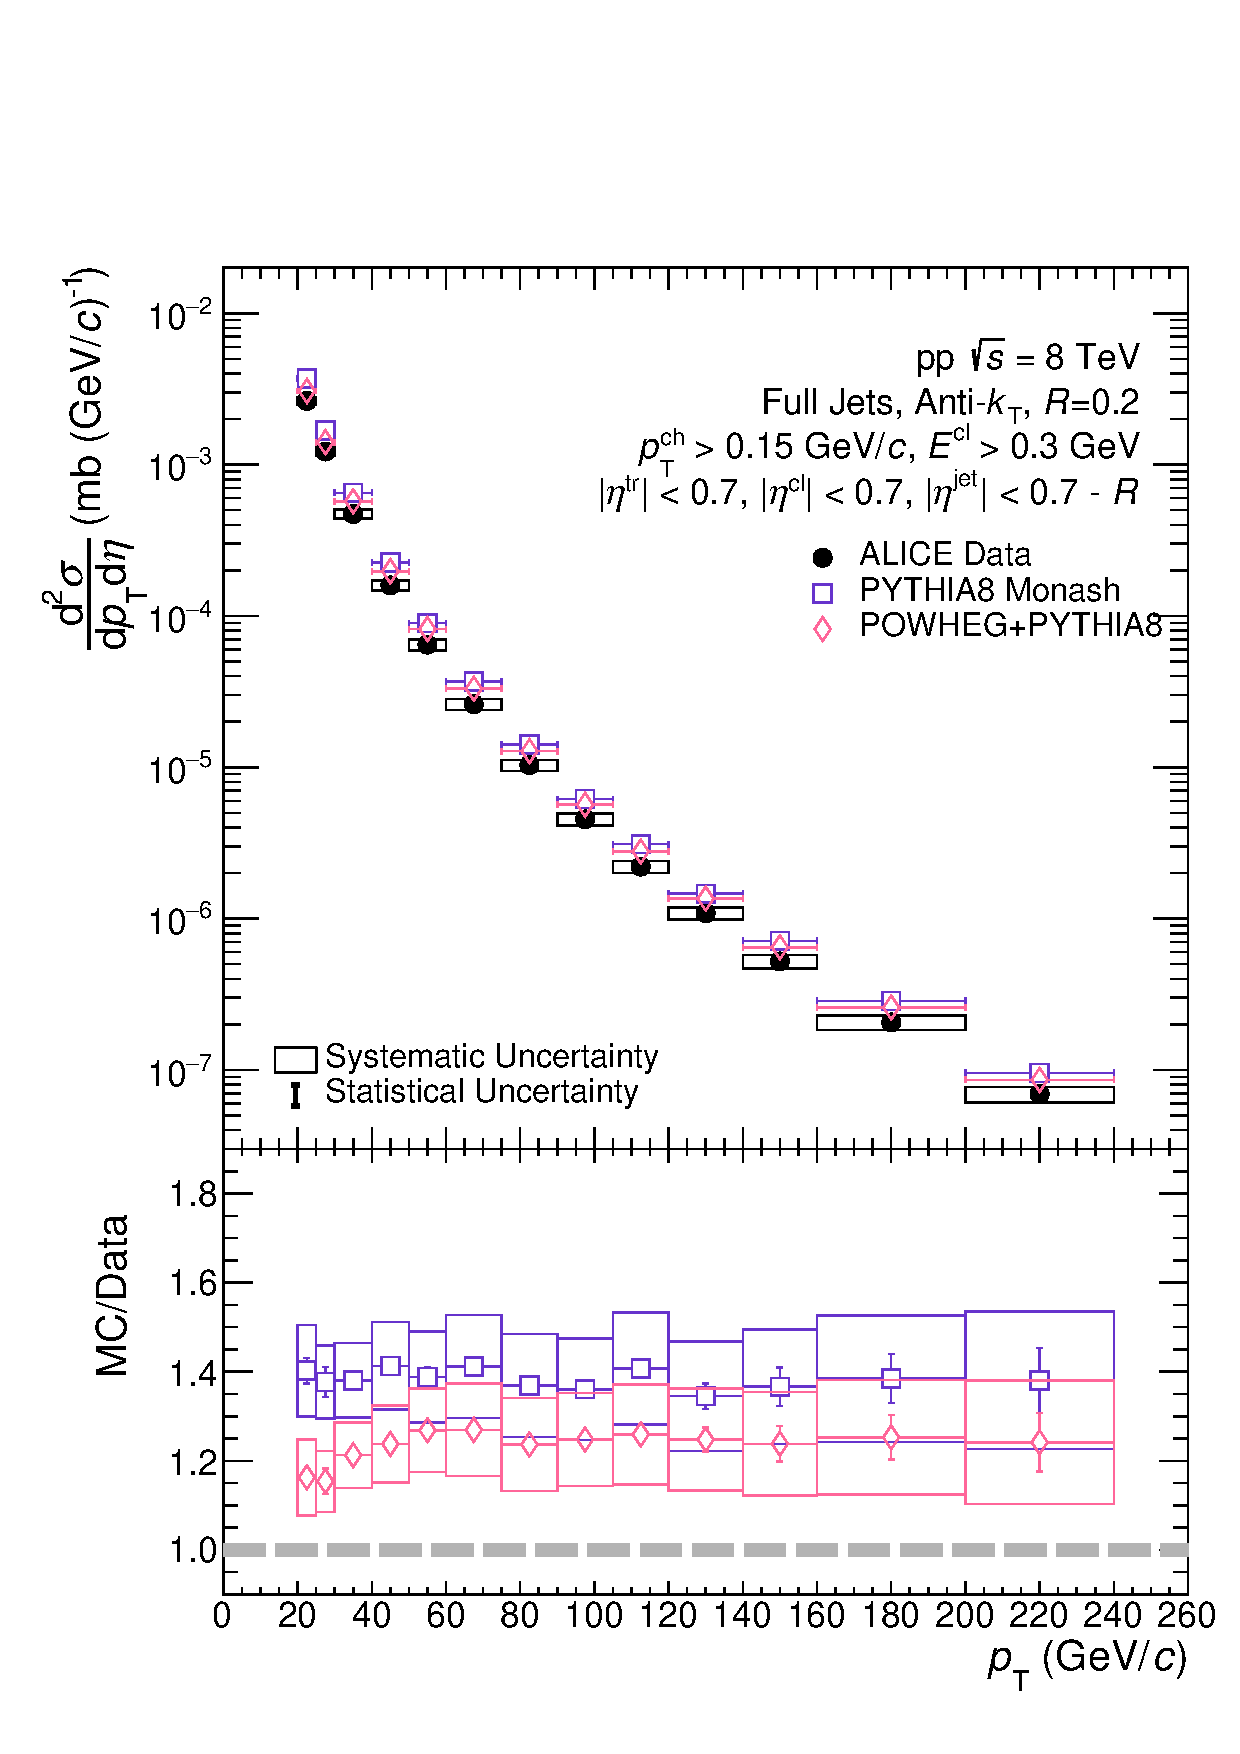
\includegraphics[width=7.5cm]{figures/MCGen/MCComp_R02_nooutlier.pdf}
        \vfill\null
        \columnbreak
            \includegraphics[width=7.5cm]{figures/MCGen/MCComp_R06_nooutlier.pdf}
        \vfill\null
    \end{multicols}
    \caption{Comparison to PYTHIA8 for jet radii 0.2 and 0.6.}
    \label{fig:MCGen}
\end{figure}

\begin{figure}
    \centering
    \begin{multicols}{2}
            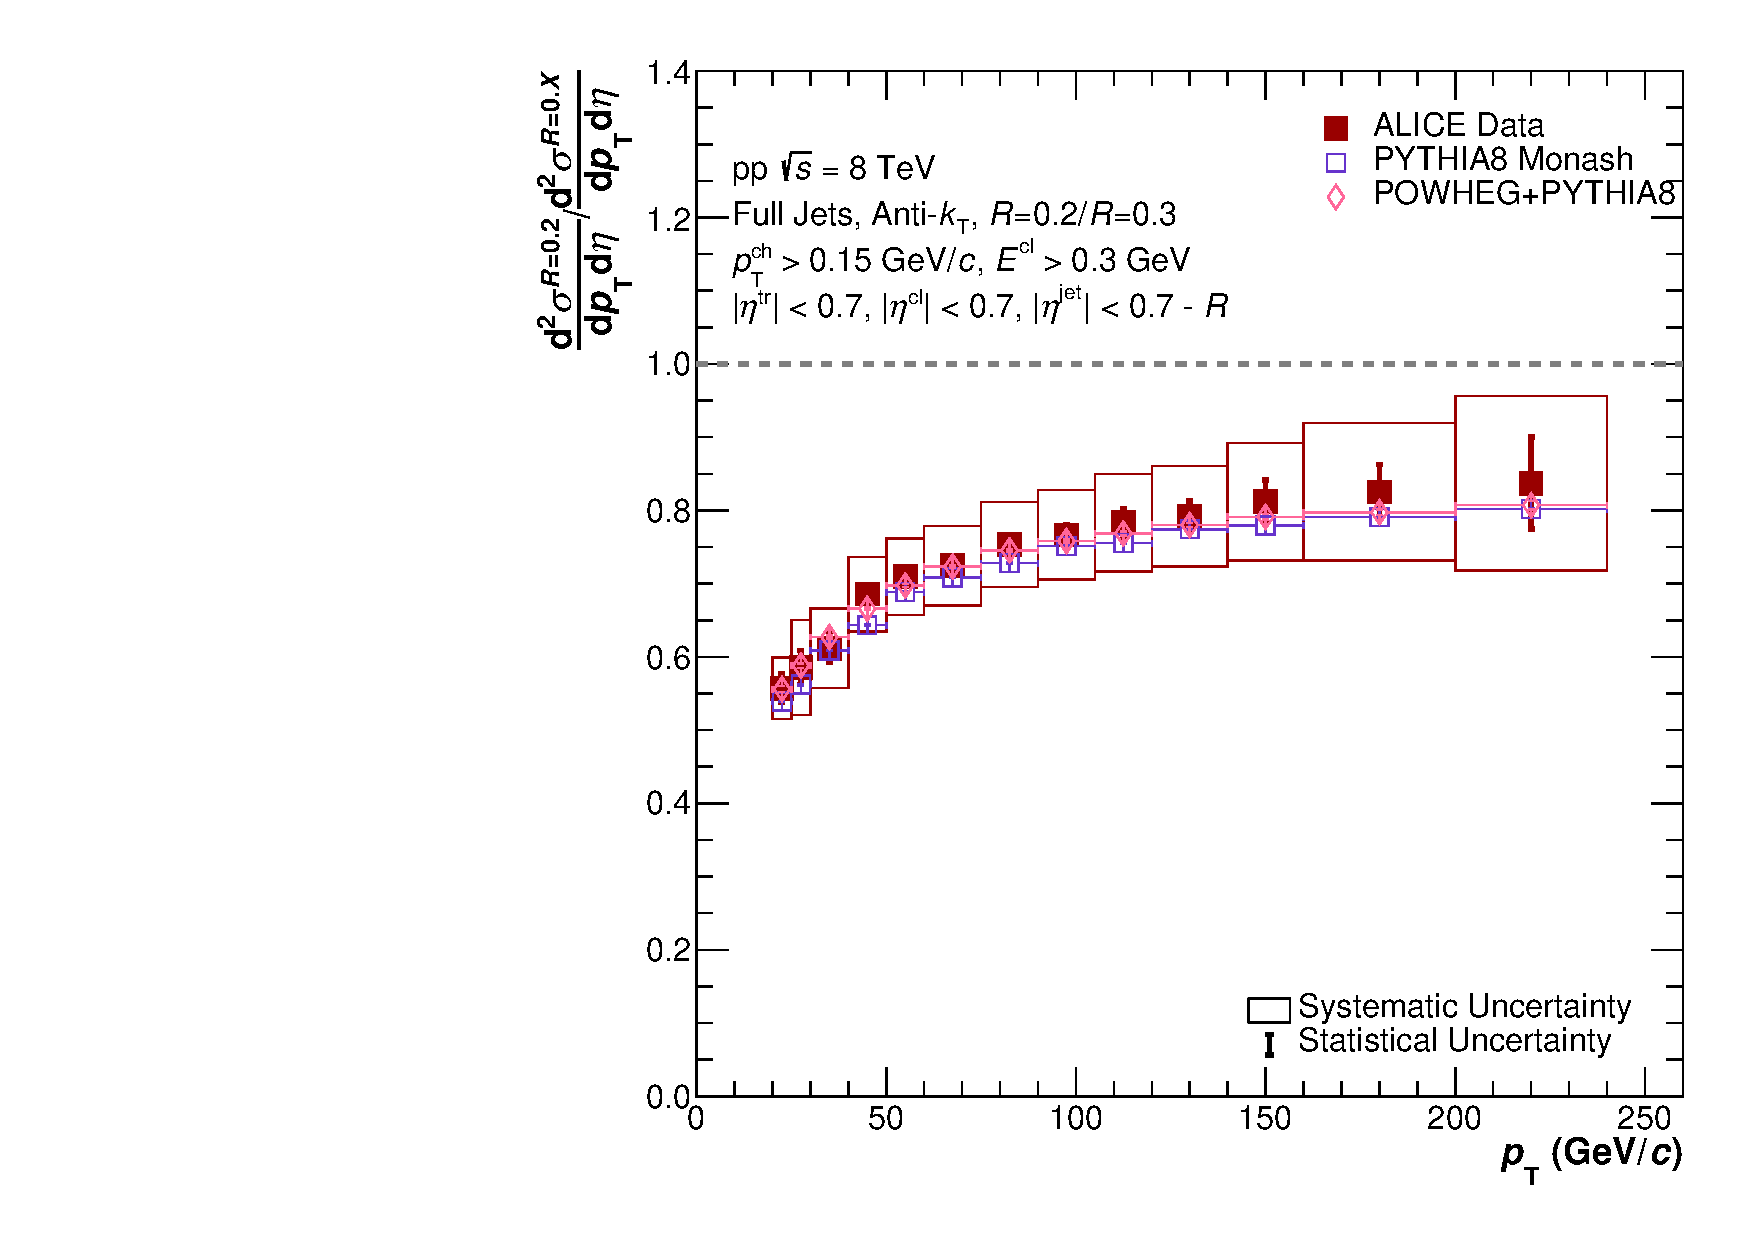
\includegraphics[width=7.5cm]{figures/MCGen/MCComp_Ratio_R0302_nooutlier.pdf}
        \vfill\null
        \columnbreak
            \includegraphics[width=7.5cm]{figures/MCGen/MCComp_Ratio_R0602_nooutlier.pdf}
        \vfill\null
    \end{multicols}
    \caption{Comparison to PYTHIA8 for ratios of jet radii 0.2/0.3 and 0.2/0.6.}
    \label{fig:MCGen_Ratio}
\end{figure}

\begin{figure}
    \centering
    \begin{multicols}{2}
            \includegraphics[width=7.5cm]{figures/MCGen/ratioDataMC/ratio_simdata_R02_nooutlier.pdf}
        \vfill\null
        \columnbreak
            \includegraphics[width=7.5cm]{figures/MCGen/ratioDataMC/ratio_simdata_R06_nooutlier.pdf}
        \vfill\null
    \end{multicols}
    \caption{Ratio of PYTHIA8 simulation to ALICE data for jet radii 0.2 and 0.6.}
    \label{fig:MCGen_RatioDataMC}
\end{figure}\clearpage{}



\begin{appendix}

\clearpage{}\section{Software Version \& Input Data}
\label{sec:software}
In the following, the software versions and train runs are listed which have been used to generate the results shown in this note. All trains were run on GA\_pp\_AOD for data and GA\_pp\_MC\_AOD for MC:

Data:
\begin{enumerate}
    \item Default for final results
    \begin{enumerate}
        \item AliPhysics Version: vAN-20221214\_O2-1
        \item Train: 2423
    \end{enumerate}
    \item Default for systematics
    \begin{enumerate}
        \item AliPhysics Version: vAN-20221214\_O2-1
        \item Train: 2422
    \end{enumerate}
    \item Seed/Cell 275/75
    \begin{enumerate}
        \item AliPhysics Version: vAN-20220302\_ROOT6-1
        \item Train: 2230
    \end{enumerate}
    \item Seed/Cell 350/100
    \begin{enumerate}
        \item AliPhysics Version: vAN-20220302\_ROOT6-1
        \item Train: 2231
    \end{enumerate}
    \item 5x5 Clusterizer
    \begin{enumerate}
        \item AliPhysics Version: vAN-20220307\_ROOT6-1
        \item Train: 2245
    \end{enumerate}
    \item 3x3 Clusterizer
    \begin{enumerate}
        \item AliPhysics Version: vAN-20220307\_ROOT6-1
        \item Train: 2246
    \end{enumerate}
    \item Hadronic correction, F = 0.7
    \begin{enumerate}
        \item AliPhysics Version: vAN-20220313\_ROOT6-1
        \item Train: 2256
    \end{enumerate}
    \item Hadronic correction, MIP
    \begin{enumerate}
        \item AliPhysics Version: vAN-20220313\_ROOT6-1
        \item Train: 2257
    \end{enumerate}
    \item Max track \pT
    \begin{enumerate}
        \item AliPhysics Version: vAN-20221027\_O2-1
        \item Train: 2386
    \end{enumerate}
    \item Max cluster E
    \begin{enumerate}
        \item AliPhysics Version: vAN-20221027\_O2-1
        \item Train: 2385
    \end{enumerate}
    \item Q/\pT shift
    \begin{enumerate}
        \item AliPhysics Version: vAN-20230201\_O2-1
        \item Train: 2440
    \end{enumerate}
    \item Tracking
    \begin{enumerate}
        \item AliPhysics Version: vAN-20221214\_O2-1
        \item Train: 2422
    \end{enumerate}
\end{enumerate}

MC:
\begin{enumerate}
    \item Default for final results
    \begin{enumerate}
        \item AliPhysics Version: vAN-20221214\_O2-1, vAN-20230111\_O2-1
        \item Train: 5486, 5517
    \end{enumerate}
    \item Default for systematics
    \begin{enumerate}
        \item AliPhysics Version: vAN-20221214\_O2-1, vAN-20230111\_O2-1
        \item Train: 5481, 5485
    \end{enumerate}
    \item Seed/Cell 275/75
    \begin{enumerate}
        \item AliPhysics Version: vAN-20220328\_ROOT6-1
        \item Train: 5053, 5054
    \end{enumerate}
    \item Seed/Cell 350/100
    \begin{enumerate}
        \item AliPhysics Version: vAN-20220328\_ROOT6-1
        \item Train: 5055, 5056
    \end{enumerate}
    \item 5x5 Clusterizer
    \begin{enumerate}
        \item AliPhysics Version: vAN-20220318\_ROOT6-1
        \item Train: 5033, 5034
    \end{enumerate}
    \item 3x3 Clusterizer
    \begin{enumerate}
        \item AliPhysics Version: vAN-20220318\_ROOT6-1
        \item Train: 5031, 5032
    \end{enumerate}
    \item Hadronic correction, F = 0.7
    \begin{enumerate}
        \item AliPhysics Version: vAN-20220313\_ROOT6-1
        \item Train: 5019, 5020
    \end{enumerate}
    \item Hadronic correction, MIP
    \begin{enumerate}
        \item AliPhysics Version: vAN-20220313\_ROOT6-1
        \item Train: 5021, 5022
    \end{enumerate}
    \item Max track \pT
    \begin{enumerate}
        \item AliPhysics Version: vAN-20221028\_O2-1, vAN-20221114\_O2-1
        \item Train: 5381, 5400-5403
    \end{enumerate}
    \item Max cluster E
    \begin{enumerate}
        \item AliPhysics Version: vAN-20221027\_O2-1, vAN-20221114\_O2-1, vAN-20221121\_O2-1
        \item Train: 5376, 5410-5412, 5420
    \end{enumerate}
    \item Q/\pT shift
    \begin{enumerate}
        \item AliPhysics Version: vAN-20221214\_O2-1, vAN-20230111\_O2-1 
        \item Train: 5481, 5485
    \end{enumerate}
    \item Tracking
    \begin{enumerate}
        \item AliPhysics Version: vAN-20220302\_ROOT6-1
        \item Train: 4940, 4941
    \end{enumerate}
\end{enumerate}

Offline software used:
\begin{enumerate}
    \item[-] QA Software: https://gitlab.cern.ch/alice-pcg/AnalysisSoftware
    \item[-] Post-Processing Software: https://github.com/aschmier/SpectrumPostProcessing
    \item[-] Unfolding and Energy Scale Software: https://github.com/aschmier/SubstructureAnalysis (Derived from: https://github.com/mfasDa/SubstructureAnalysis)
\end{enumerate}

\newpage

\section{List of Good Runs}
\label{sec:goodRuns}
\subsection{LHC12a-i, MB INT7}
\label{subsec:goodRuns12}

\begin{table}[h!]
	\hspace*{-0.2cm}
	\small
	\centering
	\begin{tabular}{ll}  
	    \toprule
	    \textbf{LHC12a - Good Runs INT7} \\ \midrule
		176715, 176730, 176749, 176752, 176753, 176849, 176854, 176859, 176924, 176926, \\ \midrule
		176927, 176929, 177011 \\
		\bottomrule
	\end{tabular}
	\caption{Runs used in this analysis for LHC12a, minimum bias trigger INT7. The set of runs is identical for data and corresponding Monte Carlo productions that are used.}
	\label{tab:runs12a}
\end{table}

\begin{table}[h!]
	\hspace*{-0.2cm}
	\small
	\centering
	\begin{tabular}{ll}  
	    \toprule
	    \textbf{LHC12b - Good Runs INT7} \\ \midrule
		177580, 177592, 177597, 177612, 177620, 177624, 177671, 177679, 177680, 177681, \\ \midrule
		177682, 177798, 177799, 177802, 177804, 177805, 177942 \\
		\bottomrule
	\end{tabular}
	\caption{Runs used in this analysis for LHC12b, minimum bias trigger INT7. The set of runs is identical for data and corresponding Monte Carlo productions that are used.}
	\label{tab:runs12b}
\end{table}

\begin{table}[h!]
	\hspace*{-0.2cm}
	\small
	\centering
	\begin{tabular}{ll}  
	    \toprule
	    \textbf{LHC12c - Good Runs INT7} \\ \midrule
		179569, 179571, 179584, 179585, 179591, 179618, 179621, 179639, 179796, 179803,  \\ \midrule
		179806, 179858, 179859, 179916, 179917, 179918, 179919, 179920, 180000, 180042,  \\ \midrule
		180044, 180129, 180130, 180131, 180132, 180133, 180199, 180200, 180500, 180501,  \\ \midrule 
		180515, 180517, 180561, 180564, 180567, 180569, 180716, 180717, 180719, 180720,  \\ \midrule 
		182017, 182018, 182022, 182023, 182106, 182110, 182111, 182207, 182289, 182295,  \\ \midrule 
		182297, 182299, 182300, 182302, 182322, 182323, 182324, 182325, 182624, 182635,  \\ \midrule 
		182684, 182686, 182687, 182691, 182692, 182724, 182725, 182728, 182729, 182730,  \\ \midrule 
		182741, 182744 \\
		\bottomrule
	\end{tabular}
	\caption{Runs used in this analysis for LHC12c, minimum bias trigger INT7. The set of runs is identical for data and corresponding Monte Carlo productions that are used.}
	\label{tab:runs12c}
\end{table}

\newpage
	////////////////////////////////////////////////////////////////////////////////////////
\begin{table}[h!]
	\hspace*{-0.2cm}
	\small
	\centering
	\begin{tabular}{ll}  
	    \toprule
	    \textbf{LHC12d - Good Runs INT7} \\ \midrule
	    183913, 183916, 183932, 183933, 183934, 183935, 183936, 183937, 183938, 183942,  \\ \midrule
	    183946, 184126, 184127, 184131, 184132, 184134, 184135, 184137, 184138, 184140,  \\ \midrule
	    184144, 184145, 184147, 184183, 184188, 184208, 184209, 184210, 184215, 184216,  \\ \midrule
	    184371, 184383, 184389, 184673, 184678, 184682, 184687, 184784, 184786, 185029,  \\ \midrule
	    185031, 185116, 185126, 185127, 185132, 185133, 185134, 185157, 185160, 185164,  \\ \midrule
	    185189, 185196, 185198, 185203, 185206, 185208, 185217, 185221, 185282, 185284,  \\ \midrule
	    185289, 185291, 185292, 185293, 185296, 185299, 185300, 185302, 185303, 185349,  \\ \midrule
	    185350, 185351, 185356, 185359, 185360, 185361, 185362, 185363, 185368, 185371,  \\ \midrule
	    185375, 185378, 185461, 185465, 185474, 185582, 185583, 185588, 185589, 185659,  \\ \midrule
	    185687, 185738, 185764, 185765, 185768, 185775, 185776, 185778, 185784, 186007,  \\ \midrule
	    186009, 186011, 186163, 186164, 186165, 186167, 186205, 186208, 186319, 186320 \\
		\bottomrule
	\end{tabular}
	\caption{Runs used in this analysis for LHC12d, minimum bias trigger INT7. The set of runs is identical for data and corresponding Monte Carlo productions that are used.}
	\label{tab:runs12d}
\end{table}

\begin{table}[h!]
	\hspace*{-0.2cm}
	\small
	\centering
	\begin{tabular}{ll}  
	    \toprule
	    \textbf{LHC12f - Good Runs INT7} \\ \midrule
		186668, 186688, 186689, 186690, 186692, 186694, 186811, 186814, 186937, 186938,  \\ \midrule
		186939, 186966, 186969, 186990, 186992, 186994, 187143, 187145, 187146, 187147,  \\ \midrule
		187148, 187149, 187150, 187151, 187152, 187202, 187203, 187339, 187340, 187341,  \\ \midrule
		187487, 187488, 187489, 187510, 187623, 187624, 187627, 187656, 187698, 187739,  \\ \midrule
		187749, 187783, 187785, 187791, 187796, 188093, 188101 \\
		\bottomrule
	\end{tabular}
	\caption{Runs used in this analysis for LHC12f, minimum bias trigger INT7. The set of runs is identical for data and corresponding Monte Carlo productions that are used.}
	\label{tab:runs12f}
\end{table}

\newpage

\begin{table}[h!]
	\hspace*{-0.2cm}
	\small
	\centering
	\begin{tabular}{ll}  
	    \toprule
	    \textbf{LHC12h - Good Runs INT7} \\ \midrule
		189306, 189310, 189315, 189316, 189350, 189351, 189352, 189353, 189400, 189407,  \\ \midrule
		189409, 189410, 189411, 189577, 189578, 189602, 189603, 189605, 189610, 189611,  \\ \midrule
		189612, 189616, 189621, 189623, 189647, 189648, 189650, 189654, 189656, 189658,  \\ \midrule
		189659, 189696, 189697, 189698, 190150, 190209, 190210, 190212, 190213, 190214,  \\ \midrule
		190215, 190216, 190240, 190303, 190305, 190307, 190335, 190337, 190338, 190340,  \\ \midrule
		190341, 190342, 190344, 190386, 190388, 190389, 190390, 190392, 190393, 190416,  \\ \midrule
		190417, 190418, 190419, 190421, 190422, 190424, 190425, 190895, 190898, 190903,  \\ \midrule
		190904, 190968, 190970, 190974, 190975, 190979, 190981, 190983, 190984, 191129,  \\ \midrule
		191227, 191229, 191230, 191231, 191245, 191247, 191248, 191450, 191451, 192072,  \\ \midrule
		192073, 192075, 192128, 192136, 192140, 192141, 192172, 192174, 192177, 192194,  \\ \midrule
		192197, 192199, 192200, 192201, 192202, 192205, 192246, 192344, 192347, 192348,  \\ \midrule
		192349, 192415, 192417, 192453, 192461, 192468, 192471, 192492, 192499, 192505,  \\ \midrule
		192510, 192535, 192542, 192548, 192551, 192729, 192731, 192732 \\
		\bottomrule
	\end{tabular}
	\caption{Runs used in this analysis for LHC12h, minimum bias trigger INT7. The set of runs is identical for data and corresponding Monte Carlo productions that are used.}
	\label{tab:runs12h}
\end{table}

\begin{table}[h!]
	\hspace*{-0.2cm}
	\small
	\centering
	\begin{tabular}{ll}  
	    \toprule
	    \textbf{LHC12i - Good Runs INT7} \\ \midrule
		192772, 192775, 192778, 192779, 192820, 192822, 192824, 193004, 193005, 193007,  \\ \midrule
		193008, 193010, 193011, 193014, 193047, 193049, 193051, 193092, 193093, 193094,  \\ \midrule
		193097, 193148, 193155, 193156, 193187, 193188, 193189, 193194 \\
		\bottomrule
	\end{tabular}
	\caption{Runs used in this analysis for LHC12i, minimum bias trigger INT7. The set of runs is identical for data and corresponding Monte Carlo productions that are used.}
	\label{tab:runs12i}
\end{table}

\newpage

\subsection{LHC12c-i, EMC L0, INT7}	
\label{subsec:runsL0}

\begin{table}[h!]
	\hspace*{-0.2cm}
	\small
	\centering
	\begin{tabular}{ll}  
	    \toprule
	    \textbf{LHC12c - Good Runs EMC L0, INT7} \\ \midrule
		179796, 179803, 179806, 179858, 179859, 179916, 179917, 179918, 179919, 179920,  \\ \midrule
		180000, 180042, 180044, 180129, 180130, 180131, 180132, 180133, 180500, 180501,  \\ \midrule
		180515, 180517, 180561, 180564, 180567, 180569, 180716, 180717, 180719, 180720,  \\ \midrule
		182017, 182018, 182022, 182023, 182106, 182110, 182111, 182207, 182289, 182295,  \\ \midrule
		182297, 182299, 182300, 182302, 182322, 182323, 182324, 182325, 182624, 182635,  \\ \midrule
		182684, 182686, 182687, 182691, 182692, 182724, 182725, 182728, 182729, 182730,  \\ \midrule
		182741, 182744 \\
		\bottomrule
	\end{tabular}
	\caption{Runs used in this analysis for LHC12c, EMC L0, INT7.}
	\label{tab:runs12cL0}
\end{table}

\begin{table}[h!]
	\hspace*{-0.2cm}
	\small
	\centering
	\begin{tabular}{ll}  
	    \toprule
	    \textbf{LHC12d - Good Runs EMC L0, INT7} \\ \midrule
		183913, 183916, 183932, 183933, 183934, 183935, 183936, 183937, 183938, 183942,  \\ \midrule
		183946, 184126, 184127, 184131, 184132, 184134, 184135, 184137, 184138, 184140,  \\ \midrule
		184144, 184145, 184147, 184183, 184188, 184208, 184209, 184210, 184215, 184216,  \\ \midrule
		184371, 184383, 184389, 184673, 184678, 184682, 184687, 184784, 184786, 185029,  \\ \midrule
		185031, 185116, 185126, 185127, 185132, 185133, 185134, 185157, 185160, 185164,  \\ \midrule
		185189, 185196, 185198, 185203, 185206, 185208, 185217, 185221, 185282, 185284,  \\ \midrule
		185289, 185292, 185293, 185296, 185299, 185300, 185302, 185303, 185349, 185350,  \\ \midrule
		185351, 185356, 185359, 185360, 185361, 185362, 185363, 185368, 185371, 185375,  \\ \midrule
		185378, 185461, 185465, 185474, 185582, 185583, 185588, 185589, 185659, 185687,  \\ \midrule
		185738, 185764, 185765, 185768, 185775, 185776, 185778, 185784, 186163, 186164,  \\ \midrule
		186165, 186167, 186205, 186208, 186319, 186320 \\
		\bottomrule
	\end{tabular}
	\caption{Runs used in this analysis for LHC12d, EMC L0, INT7}
	\label{tab:runs12dL0}
\end{table}

\begin{table}[h!]
	\hspace*{-0.2cm}
	\small
	\centering
	\begin{tabular}{ll}  
	    \toprule
	    \textbf{LHC12f - Good Runs EMC L0, INT7} \\ \midrule
		186668, 186688, 186689, 186690, 186692, 186694, 186811, 186814, 186937, 186938,  \\ \midrule
		186939, 186966, 186969, 186990, 186992, 186994, 187143, 187145, 187146, 187147,  \\ \midrule
		187148, 187149, 187150, 187151, 187152, 187202, 187203, 187339, 187340, 187341,  \\ \midrule
		187487, 187488, 187489, 187510, 187623, 187624, 187627, 187656, 187698, 187739,  \\ \midrule
		187749, 187783, 187785, 187791, 187796, 188093, 188101 \\
		\bottomrule
	\end{tabular}
	\caption{Runs used in this analysis for LHC12f, EMC L0, INT7.}
	\label{tab:runs12fL0}
\end{table}

\newpage

\begin{table}[h!]
	\hspace*{-0.2cm}
	\small
	\centering
	\begin{tabular}{ll}  
	    \toprule
	    \textbf{LHC12h - Good Runs EMC L0, INT7} \\ \midrule
		190209, 190210, 190212, 190213, 190214, 190215, 190216, 190240, 190303, 190305,  \\ \midrule
		190307, 190335, 190337, 190338, 190340, 190341, 190342, 190344, 190386, 190388,  \\ \midrule
		190389, 190390, 190392, 190393, 190416, 190417, 190418, 190419, 190421, 190422,  \\ \midrule
		190424, 190425, 191129, 191227, 191230, 191231, 191245, 191247, 191248, 191450,  \\ \midrule
		191451, 192072, 192073, 192075, 192128, 192136, 192140, 192141, 192172, 192174,  \\ \midrule
		192177, 192194, 192197, 192199, 192200, 192201, 192202, 192205, 192344, 192347,  \\ \midrule
		192348, 192349, 192415, 192417, 192453, 192461, 192468, 192471, 192492, 192499,  \\ \midrule
		192535, 192542, 192548, 192551, 192729, 192731, 192732 \\
		\bottomrule
	\end{tabular}
	\caption{Runs used in this analysis for LHC12h, EMC L0, INT7.}
	\label{tab:runs12hL0}
\end{table}

\begin{table}[h!]
	\hspace*{-0.2cm}
	\small
	\centering
	    \begin{tabular}{ll}  
	    \toprule
	    \textbf{LHC12i - Good Runs EMC L0, INT7} \\ \midrule
		192775, 192778, 192779, 192822, 192824, 193004, 193005, 193007, 193008, 193010,  \\ \midrule
		193011, 193014, 193049, 193051, 193092, 193093, 193094, 193097, 193148, 193155,  \\ \midrule
		193156, 193187, 193188, 193189, 193194 \\
		\bottomrule
	\end{tabular}
	\caption{Runs used in this analysis for LHC12i, EMC L0, INT7.}
	\label{tab:runs12iL0}
\end{table}

\newpage

\subsection{LHC12c-i, EMC L1, INT7}	
\label{subsec:runsL1}

\begin{table}[h!]
	\hspace*{-0.2cm}
	\small
	\centering
	\begin{tabular}{ll}  
	    \toprule
	    \textbf{LHC12c - Good Runs EMC L1, INT7} \\ \midrule
		179806, 179859, 179916, 179917, 179918, 179919, 179920, 180000, 180042, 180044,  \\ \midrule
		180129, 180130, 180131, 180132, 180133, 180500, 180501, 180515, 180517, 180561,  \\ \midrule
		180564, 180567, 180569, 180716, 180717, 180719, 180720, 182017, 182018, 182022,  \\ \midrule
		182023, 182106, 182110, 182111, 182207, 182289, 182295, 182297, 182299, 182300,  \\ \midrule
		182302, 182322, 182323, 182324, 182325, 182624, 182635, 182684, 182686, 182687,  \\ \midrule
		182691, 182692, 182724, 182725, 182728, 182729, 182730, 182741, 182744 \\
		\bottomrule
	\end{tabular}
	\caption{Runs used in this analysis for LHC12c, EMC L1, INT7.}
	\label{tab:runs12cL1}
\end{table}

\begin{table}[h!]
	\hspace*{-0.2cm}
	\small
	\centering
	\begin{tabular}{ll}  
	    \toprule
	    \textbf{LHC12d - Good Runs EMC L1, INT7} \\ \midrule
		183913, 183916, 183932, 183933, 183934, 183935, 183936, 183937, 183938, 183942,  \\ \midrule
		183946, 184126, 184127, 184131, 184132, 184134, 184135, 184137, 184138, 184140,  \\ \midrule
		184144, 184145, 184147, 184183, 184188, 184208, 184209, 184210, 184215, 184216,  \\ \midrule
		184371, 184383, 184389, 184673, 184678, 184682, 184687, 184784, 184786, 185029,  \\ \midrule
		185031, 185116, 185126, 185127, 185132, 185133, 185134, 185157, 185160, 185164,  \\ \midrule
		185189, 185196, 185198, 185203, 185206, 185208, 185217, 185221, 185282, 185284,  \\ \midrule
		185289, 185292, 185293, 185296, 185299, 185300, 185302, 185303, 185349, 185350,  \\ \midrule
		185351, 185356, 185359, 185360, 185361, 185362, 185363, 185368, 185371, 185375,  \\ \midrule
		185378, 185461, 185465, 185582, 185583, 185588, 185589, 185659, 185687, 185738,  \\ \midrule
		185764, 185765, 185768, 185775, 185776, 185778, 185784, 186163, 186164, 186165,  \\ \midrule
		186167, 186205, 186208, 186319, 186320 \\
		\bottomrule
	\end{tabular}
	\caption{Runs used in this analysis for LHC12d, EMC L1, INT7.}
	\label{tab:runs12dL1}
\end{table}

\begin{table}[h!]
	\hspace*{-0.2cm}
	\small
	\centering
	\begin{tabular}{ll}  
	    \toprule
	    \textbf{LHC12f - Good Runs EMC L1, INT7} \\ \midrule
		186668, 186688, 186689, 186690, 186692, 186694, 186811, 186814, 186937, 186939,  \\ \midrule
		186966, 186969, 186990, 186992, 186994, 187143, 187145, 187146, 187148, 187149,  \\ \midrule
		187150, 187151, 187152, 187202, 187203, 187339, 187340, 187341, 187487, 187488,  \\ \midrule
		187489, 187510, 187623, 187624, 187627, 187656, 187698, 187739, 187749, 187783,  \\ \midrule
		187785, 187791, 187796, 188093, 188101 \\
		\bottomrule
	\end{tabular}
	\caption{Runs used in this analysis for LHC12f, EMC L1, INT7.}
	\label{tab:runs12fL1}
\end{table}

\newpage

\begin{table}[h!]
	\hspace*{-0.2cm}
	\small
	\centering
	\begin{tabular}{ll}  
	    \toprule
	    \textbf{LHC12h - Good Runs EMC L1, INT7} \\ \midrule
		189603, 189605, 189610, 189611, 189612, 189616, 189621, 189623, 189647, 189648,  \\ \midrule
		189650, 189654, 189656, 189658, 189659, 189696, 189697, 189698, 190209, 190210,  \\ \midrule
		190212, 190213, 190214, 190215, 190216, 190240, 190303, 190305, 190307, 190335,  \\ \midrule
		190337, 190338, 190340, 190341, 190342, 190344, 190386, 190388, 190389, 190390,  \\ \midrule
		190392, 190393, 190416, 190417, 190418, 190419, 190421, 190422, 190424, 190425,  \\ \midrule
		191129, 191227, 191230, 191231, 191245, 191247, 191248, 191450, 191451, 192072,  \\ \midrule
		192073, 192075, 192128, 192136, 192140, 192141, 192172, 192174, 192177, 192194,  \\ \midrule
		192197, 192199, 192200, 192201, 192202, 192205, 192344, 192347, 192348, 192349,  \\ \midrule
		192415, 192417, 192453, 192461, 192468, 192471, 192492, 192499, 192535, 192542,  \\ \midrule
		192548, 192551, 192729, 192731, 192732 \\
		\bottomrule
	\end{tabular}
	\caption{Runs used in this analysis for LHC12h, EMC L1, INT7.}
	\label{tab:runs12hL1}
\end{table}

\begin{table}[h!]
	\hspace*{-0.2cm}
	\small
	\centering
	\begin{tabular}{ll}  
	    \toprule
	    \textbf{LHC12i - Good Runs EMC L1, INT7} \\ \midrule
		192772, 192775, 192778, 192779, 192820, 192822, 192824, 193004, 193005, 193007,  \\ \midrule
		193008, 193010, 193011, 193014, 193047, 193049, 193051, 193092, 193093, 193094,  \\ \midrule
		193097 \\
		\bottomrule
	\end{tabular}
	\caption{Runs used in this analysis for LHC12i, EMC L1, INT7.}
	\label{tab:runs12iL1}
\end{table}

\newpage

\subsection{Jet-Jet Monte Carlo}	
\label{subsec:runsJJMC}

\begin{table}[h!]
	\hspace*{-0.2cm}
	\small
	\centering
	\begin{tabular}{lccccc}  
	    \toprule
		\multicolumn{6}{l}{\textbf{LHC16c2 - anchor run list for JetJet Pythia8 Monte Carlo}} \\ \midrule
		Period & LHC12c & LHC12d & LHC12f & LHC12h & LHC12i\\
		$N^{\text{EMC L1-GA}}_{\text{collected}}$ & $3.8 \cdot 10^{5}$ & $4.9 \cdot 10^{5}$ & $2.5 \cdot 10^{5}$ & $9.8 \cdot 10^{5}$ & $2.4 \cdot 10^{5}$\\ \midrule
		Runs 			 & 180720 (8.13\%) & 184215 (16.75\%) & 187488 (10.78\%) & 189616 (6.66\%) & 193051 (10.32\%) \\
		with fraction	 & 182692 (8.13\%) & 185687 (4.19\%) &  & 190393 (5.90\%) &  \\
		of generated	 &  &  &  & 192073 (14.58\%) &  \\
		statistics (\%)	 &  &  &  & 192349 (14.58\%) &  \\
		\bottomrule
	\end{tabular}
	\caption{List of runs to which JetJet Monte Carlo LHC16c2 has been anchored to. The basis for this selection is the good trigger runlist, LHC12c-i, EMC L1-GA, INT7. The number of total triggers has been determined and one anchor run per approximately $ 2.5 \cdot 10^{6}$ events has been defined. Furthermore, it has been ensured that varying detector acceptance is properly reflected in the percentage of events to be generated for each anchor run. For example, if one or even multiple RCUs of EMCal were switched off during some runs in data taking, it has properly been considered by grouping the runs according to detector acceptance and summing up the respective number of events collected using L1-GA trigger. Then the fraction of events for each group could be calculated according to the full sample of collected EMC L1-GA triggers, which are also displayed in the table above.}
	\label{tab:runsJetJet}
\end{table}

\newpage

\section{NEF, \texorpdfstring{Z\textsubscript{ch}}{Zch}, and \texorpdfstring{Z\textsubscript{ne}}{Zne} for Other Radii}
\label{sec:appendixTriggerBias}


\begin{figure}[h!]
    \centering
    \subfigure{\label{fig:NEF_6-10GeV_R02}\includegraphics[width=.45\textwidth]{figures/NEF/All/hNEF_6-10GeV_R02.pdf}}
    \qquad
    \subfigure{\label{fig:NEF_10-20GeV_R02}\includegraphics[width=.45\textwidth]{figures/NEF/All/hNEF_10-20GeV_R02.pdf}}\\
    \subfigure{\label{fig:NEF_20-30GeV_R02}\includegraphics[width=.45\textwidth]{figures/NEF/All/hNEF_20-30GeV_R02.pdf}}
    \qquad
    \subfigure{\label{fig:NEF_30-60GeV_R02}\includegraphics[width=.45\textwidth]{figures/NEF/All/hNEF_30-60GeV_R02.pdf}}\\
    \subfigure{\label{fig:NEF_60-100GeV_R02}\includegraphics[width=.45\textwidth]{figures/NEF/All/hNEF_60-100GeV_R02.pdf}}
    \qquad
    \subfigure{\label{fig:NEF_100-200GeV_R02}\includegraphics[width=.45\textwidth]{figures/NEF/All/hNEF_100-160GeV_R02.pdf}}\\
    \subfigure{\label{fig:NEF_200-350GeV_R02}\includegraphics[width=.45\textwidth]{figures/NEF/All/hNEF_160-240GeV_R02.pdf}}
    \caption{NEF for R=0.2 jets in several bins of \pT}
    \label{fig:appendixTriggerBiasNEFR02}
\end{figure}

\newpage

\begin{figure}[h!]
    \centering
    \subfigure{\label{fig:Zch_6-10GeV_R02}\includegraphics[width=.45\textwidth]{figures/Zch/All/hZch_6-10GeV_R02.pdf}}
    \qquad
    \subfigure{\label{fig:Zch_10-20GeV_R02}\includegraphics[width=.45\textwidth]{figures/Zch/All/hZch_10-20GeV_R02.pdf}}\\
    \subfigure{\label{fig:Zch_20-30GeV_R02}\includegraphics[width=.45\textwidth]{figures/Zch/All/hZch_20-30GeV_R02.pdf}}
    \qquad
    \subfigure{\label{fig:Zch_30-60GeV_R02}\includegraphics[width=.45\textwidth]{figures/Zch/All/hZch_30-60GeV_R02.pdf}}\\
    \subfigure{\label{fig:Zch_60-100GeV_R02}\includegraphics[width=.45\textwidth]{figures/Zch/All/hZch_60-100GeV_R02.pdf}}
    \qquad
    \subfigure{\label{fig:Zch_100-200GeV_R02}\includegraphics[width=.45\textwidth]{figures/Zch/All/hZch_100-160GeV_R02.pdf}}\\
    \subfigure{\label{fig:Zch_200-350GeV_R02}\includegraphics[width=.45\textwidth]{figures/Zch/All/hZch_160-240GeV_R02.pdf}}
    \caption{Z$_{ch}$ for R=0.2 jets in several bins of \pT}
    \label{fig:TriggerBiasZchR02}
\end{figure}

\newpage

\begin{figure}[h!]
    \centering
    \subfigure{\label{fig:Zne_6-10GeV_R02}\includegraphics[width=.45\textwidth]{figures/Zne/All/hZne_6-10GeV_R02.pdf}}
    \qquad
    \subfigure{\label{fig:Zne_10-20GeV_R02}\includegraphics[width=.45\textwidth]{figures/Zne/All/hZne_10-20GeV_R02.pdf}}\\
    \subfigure{\label{fig:Zne_20-30GeV_R02}\includegraphics[width=.45\textwidth]{figures/Zne/All/hZne_20-30GeV_R02.pdf}}
    \qquad
    \subfigure{\label{fig:Zne_30-60GeV_R02}\includegraphics[width=.45\textwidth]{figures/Zne/All/hZne_30-60GeV_R02.pdf}}\\
    \subfigure{\label{fig:Zne_60-100GeV_R02}\includegraphics[width=.45\textwidth]{figures/Zne/All/hZne_60-100GeV_R02.pdf}}
    \qquad
    \subfigure{\label{fig:Zne_100-200GeV_R02}\includegraphics[width=.45\textwidth]{figures/Zne/All/hZne_100-160GeV_R02.pdf}}\\
    \subfigure{\label{fig:Zne_200-350GeV_R02}\includegraphics[width=.45\textwidth]{figures/Zne/All/hZne_160-240GeV_R02.pdf}}
    \caption{Z$_{ne}$ for R=0.2 jets in several bins of \pT}
    \label{fig:TriggerBiasZneR02}
\end{figure}

\newpage

\begin{figure}[h!]
    \centering
    \subfigure{\label{fig:NEF_6-10GeV_R03}\includegraphics[width=.45\textwidth]{figures/NEF/All/hNEF_6-10GeV_R03.pdf}}
    \qquad
    \subfigure{\label{fig:NEF_10-20GeV_R03}\includegraphics[width=.45\textwidth]{figures/NEF/All/hNEF_10-20GeV_R03.pdf}}\\
    \subfigure{\label{fig:NEF_20-30GeV_R03}\includegraphics[width=.45\textwidth]{figures/NEF/All/hNEF_20-30GeV_R03.pdf}}
    \qquad
    \subfigure{\label{fig:NEF_30-60GeV_R03}\includegraphics[width=.45\textwidth]{figures/NEF/All/hNEF_30-60GeV_R03.pdf}}\\
    \subfigure{\label{fig:NEF_60-100GeV_R03}\includegraphics[width=.45\textwidth]{figures/NEF/All/hNEF_60-100GeV_R03.pdf}}
    \qquad
    \subfigure{\label{fig:NEF_100-200GeV_R03}\includegraphics[width=.45\textwidth]{figures/NEF/All/hNEF_100-160GeV_R03.pdf}}\\
    \subfigure{\label{fig:NEF_200-350GeV_R03}\includegraphics[width=.45\textwidth]{figures/NEF/All/hNEF_160-240GeV_R03.pdf}}
    \caption{NEF for R=0.3 jets in several bins of \pT}
    \label{fig:TriggerBiasNEFR03}
\end{figure}

\newpage

\begin{figure}[h!]
    \centering
    \subfigure{\label{fig:Zch_6-10GeV_R03}\includegraphics[width=.45\textwidth]{figures/Zch/All/hZch_6-10GeV_R03.pdf}}
    \qquad
    \subfigure{\label{fig:Zch_10-20GeV_R03}\includegraphics[width=.45\textwidth]{figures/Zch/All/hZch_10-20GeV_R03.pdf}}\\
    \subfigure{\label{fig:Zch_20-30GeV_R03}\includegraphics[width=.45\textwidth]{figures/Zch/All/hZch_20-30GeV_R03.pdf}}
    \qquad
    \subfigure{\label{fig:Zch_30-60GeV_R03}\includegraphics[width=.45\textwidth]{figures/Zch/All/hZch_30-60GeV_R03.pdf}}\\
    \subfigure{\label{fig:Zch_60-100GeV_R03}\includegraphics[width=.45\textwidth]{figures/Zch/All/hZch_60-100GeV_R03.pdf}}
    \qquad
    \subfigure{\label{fig:Zch_100-200GeV_R03}\includegraphics[width=.45\textwidth]{figures/Zch/All/hZch_100-160GeV_R03.pdf}}\\
    \subfigure{\label{fig:Zch_200-350GeV_R03}\includegraphics[width=.45\textwidth]{figures/Zch/All/hZch_160-240GeV_R03.pdf}}
    \caption{Z$_{ch}$ for R=0.3 jets in several bins of \pT}
    \label{fig:TriggerBiasZchR03}
\end{figure}

\newpage

\begin{figure}[h!]
    \centering
    \subfigure{\label{fig:Zne_6-10GeV_R03}\includegraphics[width=.45\textwidth]{figures/Zne/All/hZne_6-10GeV_R03.pdf}}
    \qquad
    \subfigure{\label{fig:Zne_10-20GeV_R03}\includegraphics[width=.45\textwidth]{figures/Zne/All/hZne_10-20GeV_R03.pdf}}\\
    \subfigure{\label{fig:Zne_20-30GeV_R03}\includegraphics[width=.45\textwidth]{figures/Zne/All/hZne_20-30GeV_R03.pdf}}
    \qquad
    \subfigure{\label{fig:Zne_30-60GeV_R03}\includegraphics[width=.45\textwidth]{figures/Zne/All/hZne_30-60GeV_R03.pdf}}\\
    \subfigure{\label{fig:Zne_60-100GeV_R03}\includegraphics[width=.45\textwidth]{figures/Zne/All/hZne_60-100GeV_R03.pdf}}
    \qquad
    \subfigure{\label{fig:Zne_100-200GeV_R03}\includegraphics[width=.45\textwidth]{figures/Zne/All/hZne_100-160GeV_R03.pdf}}\\
    \subfigure{\label{fig:Zne_200-350GeV_R03}\includegraphics[width=.45\textwidth]{figures/Zne/All/hZne_160-240GeV_R03.pdf}}
    \caption{Z$_{ne}$ for R=0.3 jets in several bins of \pT}
    \label{fig:TriggerBiasZneR03}
\end{figure}

\newpage

\begin{figure}[h!]
    \centering
    \subfigure{\label{fig:NEF_6-10GeV_R04}\includegraphics[width=.45\textwidth]{figures/NEF/All/hNEF_6-10GeV_R04.pdf}}
    \qquad
    \subfigure{\label{fig:NEF_10-20GeV_R04}\includegraphics[width=.45\textwidth]{figures/NEF/All/hNEF_10-20GeV_R04.pdf}}\\
    \subfigure{\label{fig:NEF_20-30GeV_R04}\includegraphics[width=.45\textwidth]{figures/NEF/All/hNEF_20-30GeV_R04.pdf}}
    \qquad
    \subfigure{\label{fig:NEF_30-60GeV_R04}\includegraphics[width=.45\textwidth]{figures/NEF/All/hNEF_30-60GeV_R04.pdf}}\\
    \subfigure{\label{fig:NEF_60-100GeV_R04}\includegraphics[width=.45\textwidth]{figures/NEF/All/hNEF_60-100GeV_R04.pdf}}
    \qquad
    \subfigure{\label{fig:NEF_100-200GeV_R04}\includegraphics[width=.45\textwidth]{figures/NEF/All/hNEF_100-160GeV_R04.pdf}}\\
    \subfigure{\label{fig:NEF_200-350GeV_R04}\includegraphics[width=.45\textwidth]{figures/NEF/All/hNEF_160-240GeV_R04.pdf}}
    \caption{NEF for R=0.4 jets in several bins of \pT}
    \label{fig:TriggerBiasNEFR04}
\end{figure}

\newpage

\begin{figure}[h!]
    \centering
    \subfigure{\label{fig:Zch_6-10GeV_R04}\includegraphics[width=.45\textwidth]{figures/Zch/All/hZch_6-10GeV_R04.pdf}}
    \qquad
    \subfigure{\label{fig:Zch_10-20GeV_R04}\includegraphics[width=.45\textwidth]{figures/Zch/All/hZch_10-20GeV_R04.pdf}}\\
    \subfigure{\label{fig:Zch_20-30GeV_R04}\includegraphics[width=.45\textwidth]{figures/Zch/All/hZch_20-30GeV_R04.pdf}}
    \qquad
    \subfigure{\label{fig:Zch_30-60GeV_R04}\includegraphics[width=.45\textwidth]{figures/Zch/All/hZch_30-60GeV_R04.pdf}}\\
    \subfigure{\label{fig:Zch_60-100GeV_R04}\includegraphics[width=.45\textwidth]{figures/Zch/All/hZch_60-100GeV_R04.pdf}}
    \qquad
    \subfigure{\label{fig:Zch_100-200GeV_R04}\includegraphics[width=.45\textwidth]{figures/Zch/All/hZch_100-160GeV_R04.pdf}}\\
    \subfigure{\label{fig:Zch_200-350GeV_R04}\includegraphics[width=.45\textwidth]{figures/Zch/All/hZch_160-240GeV_R04.pdf}}
    \caption{Z$_{ch}$ for R=0.4 jets in several bins of \pT}
    \label{fig:TriggerBiasZchR04}
\end{figure}

\newpage

\begin{figure}[h!]
    \centering
    \subfigure{\label{fig:Zne_6-10GeV_R04}\includegraphics[width=.45\textwidth]{figures/Zne/All/hZne_6-10GeV_R04.pdf}}
    \qquad
    \subfigure{\label{fig:Zne_10-20GeV_R04}\includegraphics[width=.45\textwidth]{figures/Zne/All/hZne_10-20GeV_R04.pdf}}\\
    \subfigure{\label{fig:Zne_20-30GeV_R04}\includegraphics[width=.45\textwidth]{figures/Zne/All/hZne_20-30GeV_R04.pdf}}
    \qquad
    \subfigure{\label{fig:Zne_30-60GeV_R04}\includegraphics[width=.45\textwidth]{figures/Zne/All/hZne_30-60GeV_R04.pdf}}\\
    \subfigure{\label{fig:Zne_60-100GeV_R04}\includegraphics[width=.45\textwidth]{figures/Zne/All/hZne_60-100GeV_R04.pdf}}
    \qquad
    \subfigure{\label{fig:Zne_100-200GeV_R04}\includegraphics[width=.45\textwidth]{figures/Zne/All/hZne_100-160GeV_R04.pdf}}\\
    \subfigure{\label{fig:Zne_200-350GeV_R04}\includegraphics[width=.45\textwidth]{figures/Zne/All/hZne_160-240GeV_R04.pdf}}
    \caption{Z$_{ne}$ for R=0.4 jets in several bins of \pT}
    \label{fig:TriggerBiasZneR04}
\end{figure}

\newpage

\begin{figure}[h!]
    \centering
    \subfigure{\label{fig:NEF_6-10GeV_R05}\includegraphics[width=.45\textwidth]{figures/NEF/All/hNEF_6-10GeV_R05.pdf}}
    \qquad
    \subfigure{\label{fig:NEF_10-20GeV_R05}\includegraphics[width=.45\textwidth]{figures/NEF/All/hNEF_10-20GeV_R05.pdf}}\\
    \subfigure{\label{fig:NEF_20-30GeV_R05}\includegraphics[width=.45\textwidth]{figures/NEF/All/hNEF_20-30GeV_R05.pdf}}
    \qquad
    \subfigure{\label{fig:NEF_30-60GeV_R05}\includegraphics[width=.45\textwidth]{figures/NEF/All/hNEF_30-60GeV_R05.pdf}}\\
    \subfigure{\label{fig:NEF_60-100GeV_R05}\includegraphics[width=.45\textwidth]{figures/NEF/All/hNEF_60-100GeV_R05.pdf}}
    \qquad
    \subfigure{\label{fig:NEF_100-200GeV_R05}\includegraphics[width=.45\textwidth]{figures/NEF/All/hNEF_100-160GeV_R05.pdf}}\\
    \subfigure{\label{fig:NEF_200-350GeV_R05}\includegraphics[width=.45\textwidth]{figures/NEF/All/hNEF_160-240GeV_R05.pdf}}
    \caption{NEF for R=0.5 jets in several bins of \pT}
    \label{fig:TriggerBiasNEFR05}
\end{figure}

\newpage

\begin{figure}[h!]
    \centering
    \subfigure{\label{fig:Zch_6-10GeV_R05}\includegraphics[width=.45\textwidth]{figures/Zch/All/hZch_6-10GeV_R05.pdf}}
    \qquad
    \subfigure{\label{fig:Zch_10-20GeV_R05}\includegraphics[width=.45\textwidth]{figures/Zch/All/hZch_10-20GeV_R05.pdf}}\\
    \subfigure{\label{fig:Zch_20-30GeV_R05}\includegraphics[width=.45\textwidth]{figures/Zch/All/hZch_20-30GeV_R05.pdf}}
    \qquad
    \subfigure{\label{fig:Zch_30-60GeV_R05}\includegraphics[width=.45\textwidth]{figures/Zch/All/hZch_30-60GeV_R05.pdf}}\\
    \subfigure{\label{fig:Zch_60-100GeV_R05}\includegraphics[width=.45\textwidth]{figures/Zch/All/hZch_60-100GeV_R05.pdf}}
    \qquad
    \subfigure{\label{fig:Zch_100-200GeV_R05}\includegraphics[width=.45\textwidth]{figures/Zch/All/hZch_100-160GeV_R05.pdf}}\\
    \subfigure{\label{fig:Zch_200-350GeV_R05}\includegraphics[width=.45\textwidth]{figures/Zch/All/hZch_160-240GeV_R05.pdf}}
    \caption{Z$_{ch}$ for R=0.5 jets in several bins of \pT}
    \label{fig:TriggerBiasZchR05}
\end{figure}

\newpage

\begin{figure}[h!]
    \centering
    \subfigure{\label{fig:Zne_6-10GeV_R05}\includegraphics[width=.45\textwidth]{figures/Zne/All/hZne_6-10GeV_R05.pdf}}
    \qquad
    \subfigure{\label{fig:Zne_10-20GeV_R05}\includegraphics[width=.45\textwidth]{figures/Zne/All/hZne_10-20GeV_R05.pdf}}\\
    \subfigure{\label{fig:Zne_20-30GeV_R05}\includegraphics[width=.45\textwidth]{figures/Zne/All/hZne_20-30GeV_R05.pdf}}
    \qquad
    \subfigure{\label{fig:Zne_30-60GeV_R05}\includegraphics[width=.45\textwidth]{figures/Zne/All/hZne_30-60GeV_R05.pdf}}\\
    \subfigure{\label{fig:Zne_60-100GeV_R05}\includegraphics[width=.45\textwidth]{figures/Zne/All/hZne_60-100GeV_R05.pdf}}
    \qquad
    \subfigure{\label{fig:Zne_100-200GeV_R05}\includegraphics[width=.45\textwidth]{figures/Zne/All/hZne_100-160GeV_R05.pdf}}\\
    \subfigure{\label{fig:Zne_200-350GeV_R05}\includegraphics[width=.45\textwidth]{figures/Zne/All/hZne_160-240GeV_R05.pdf}}
    \caption{Z$_{ne}$ for R=0.5 jets in several bins of \pT}
    \label{fig:TriggerBiasZneR05}
\end{figure}

\newpage

\begin{figure}[h!]
    \centering
    \subfigure{\label{fig:NEF_6-10GeV_R06}\includegraphics[width=.45\textwidth]{figures/NEF/All/hNEF_6-10GeV_R06.pdf}}
    \qquad
    \subfigure{\label{fig:NEF_10-20GeV_R06}\includegraphics[width=.45\textwidth]{figures/NEF/All/hNEF_10-20GeV_R06.pdf}}\\
    \subfigure{\label{fig:NEF_20-30GeV_R06}\includegraphics[width=.45\textwidth]{figures/NEF/All/hNEF_20-30GeV_R06.pdf}}
    \qquad
    \subfigure{\label{fig:NEF_30-60GeV_R06}\includegraphics[width=.45\textwidth]{figures/NEF/All/hNEF_30-60GeV_R06.pdf}}\\
    \subfigure{\label{fig:NEF_60-100GeV_R06}\includegraphics[width=.45\textwidth]{figures/NEF/All/hNEF_60-100GeV_R06.pdf}}
    \qquad
    \subfigure{\label{fig:NEF_100-200GeV_R06}\includegraphics[width=.45\textwidth]{figures/NEF/All/hNEF_100-160GeV_R06.pdf}}\\
    \subfigure{\label{fig:NEF_200-350GeV_R06}\includegraphics[width=.45\textwidth]{figures/NEF/All/hNEF_160-240GeV_R06.pdf}}
    \caption{NEF for R=0.6 jets in several bins of \pT}
    \label{fig:TriggerBiasNEFR06}
\end{figure}

\newpage

\begin{figure}[h!]
    \centering
    \subfigure{\label{fig:Zch_6-10GeV_R06}\includegraphics[width=.45\textwidth]{figures/Zch/All/hZch_6-10GeV_R06.pdf}}
    \subfigure{\label{fig:Zch_10-20GeV_R06}\includegraphics[width=.45\textwidth]{figures/Zch/All/hZch_10-20GeV_R06.pdf}}\\
    \subfigure{\label{fig:Zch_20-30GeV_R06}\includegraphics[width=.45\textwidth]{figures/Zch/All/hZch_20-30GeV_R06.pdf}}
    \subfigure{\label{fig:Zch_30-60GeV_R06}\includegraphics[width=.45\textwidth]{figures/Zch/All/hZch_30-60GeV_R06.pdf}}\\
    \subfigure{\label{fig:Zch_60-100GeV_R06}\includegraphics[width=.45\textwidth]{figures/Zch/All/hZch_60-100GeV_R06.pdf}}
    \subfigure{\label{fig:Zch_100-200GeV_R06}\includegraphics[width=.45\textwidth]{figures/Zch/All/hZch_100-160GeV_R06.pdf}}\\
    \subfigure{\label{fig:Zch_200-350GeV_R06}\includegraphics[width=.45\textwidth]{figures/Zch/All/hZch_160-240GeV_R06.pdf}}
    \caption{Z$_{ch}$ for R=0.6 jets in several bins of \pT}
    \label{fig:TriggerBiasZchR06}
\end{figure}

\newpage

\begin{figure}[h!]
    \centering
    \subfigure{\label{fig:Zne_6-10GeV_R06}\includegraphics[width=.45\textwidth]{figures/Zne/All/hZne_6-10GeV_R06.pdf}}
    \qquad
    \subfigure{\label{fig:Zne_10-20GeV_R06}\includegraphics[width=.45\textwidth]{figures/Zne/All/hZne_10-20GeV_R06.pdf}}\\
    \subfigure{\label{fig:Zne_20-30GeV_R06}\includegraphics[width=.45\textwidth]{figures/Zne/All/hZne_20-30GeV_R06.pdf}}
    \subfigure{\label{fig:Zne_30-60GeV_R06}\includegraphics[width=.45\textwidth]{figures/Zne/All/hZne_30-60GeV_R06.pdf}}\\
    \subfigure{\label{fig:Zne_60-100GeV_R06}\includegraphics[width=.45\textwidth]{figures/Zne/All/hZne_60-100GeV_R06.pdf}}
    \subfigure{\label{fig:Zne_100-200GeV_R06}\includegraphics[width=.45\textwidth]{figures/Zne/All/hZne_100-160GeV_R06.pdf}}\\
    \subfigure{\label{fig:Zne_200-350GeV_R06}\includegraphics[width=.45\textwidth]{figures/Zne/All/hZne_160-240GeV_R06.pdf}}
    \caption{Z$_{ne}$ for R=0.6 jets in several bins of \pT}
    \label{fig:TriggerBiasZneR06}
\end{figure}

\newpage

\section{NEF, \texorpdfstring{Z\textsubscript{ch}}{Zch}, and \texorpdfstring{Z\textsubscript{ne}}{Zne} Ratios for Data/MC}
\label{sec:appendixTriggerBiasRatios}


\begin{figure}[h!]
    \centering
    \subfigure{\includegraphics[width=.45\textwidth]{figures/TriggerBias/NEF/hNEF_ptBin0_R02.pdf}}
    \qquad
    \subfigure{\includegraphics[width=.45\textwidth]{figures/TriggerBias/NEF/hNEF_ptBin2_R02.pdf}}\\
    \subfigure{\includegraphics[width=.45\textwidth]{figures/TriggerBias/NEF/hNEF_ptBin4_R02.pdf}}
    \qquad
    \subfigure{\includegraphics[width=.45\textwidth]{figures/TriggerBias/NEF/hNEF_ptBin1_R02.pdf}}\\
    \subfigure{\includegraphics[width=.45\textwidth]{figures/TriggerBias/NEF/hNEF_ptBin3_R02.pdf}}
    \qquad
    \subfigure{\includegraphics[width=.45\textwidth]{figures/TriggerBias/NEF/hNEF_ptBin5_R02.pdf}}
    \caption{NEF ratios of data to MC for R=0.2.}
    \label{fig:TriggerBiasRatiosNEFR02}
\end{figure}

\newpage

\begin{figure}[h!]
    \centering
    \subfigure{\includegraphics[width=.45\textwidth]{figures/TriggerBias/Zch/hZch_ptBin0_R02.pdf}}
    \qquad
    \subfigure{\includegraphics[width=.45\textwidth]{figures/TriggerBias/Zch/hZch_ptBin2_R02.pdf}}\\
    \subfigure{\includegraphics[width=.45\textwidth]{figures/TriggerBias/Zch/hZch_ptBin4_R02.pdf}}
    \qquad
    \subfigure{\includegraphics[width=.45\textwidth]{figures/TriggerBias/Zch/hZch_ptBin1_R02.pdf}}\\
    \subfigure{\includegraphics[width=.45\textwidth]{figures/TriggerBias/Zch/hZch_ptBin3_R02.pdf}}
    \qquad
    \subfigure{\includegraphics[width=.45\textwidth]{figures/TriggerBias/Zch/hZch_ptBin5_R02.pdf}}
    \caption{Z$_{ch}$ ratios of data to MC for R=0.2.}
    \label{fig:TriggerBiasRatiosZchR02}
\end{figure}

\newpage

\begin{figure}[h!]
    \centering
    \subfigure{\includegraphics[width=.45\textwidth]{figures/TriggerBias/Zne/hZne_ptBin0_R02.pdf}}
    \qquad
    \subfigure{\includegraphics[width=.45\textwidth]{figures/TriggerBias/Zne/hZne_ptBin2_R02.pdf}}\\
    \subfigure{\includegraphics[width=.45\textwidth]{figures/TriggerBias/Zne/hZne_ptBin4_R02.pdf}}
    \qquad
    \subfigure{\includegraphics[width=.45\textwidth]{figures/TriggerBias/Zne/hZne_ptBin1_R02.pdf}}\\
    \subfigure{\includegraphics[width=.45\textwidth]{figures/TriggerBias/Zne/hZne_ptBin3_R02.pdf}}
    \qquad
    \subfigure{\includegraphics[width=.45\textwidth]{figures/TriggerBias/Zne/hZne_ptBin5_R02.pdf}}
    \caption{Z$_{ne}$ ratios of data to MC for R=0.2.}
    \label{fig:TriggerBiasRatiosZneR02}
\end{figure}

\newpage

\begin{figure}[h!]
    \centering
    \subfigure{\includegraphics[width=.45\textwidth]{figures/TriggerBias/NEF/hNEF_ptBin0_R03.pdf}}
    \qquad
    \subfigure{\includegraphics[width=.45\textwidth]{figures/TriggerBias/NEF/hNEF_ptBin2_R03.pdf}}\\
    \subfigure{\includegraphics[width=.45\textwidth]{figures/TriggerBias/NEF/hNEF_ptBin4_R03.pdf}}
    \qquad
    \subfigure{\includegraphics[width=.45\textwidth]{figures/TriggerBias/NEF/hNEF_ptBin1_R03.pdf}}\\
    \subfigure{\includegraphics[width=.45\textwidth]{figures/TriggerBias/NEF/hNEF_ptBin3_R03.pdf}}
    \qquad
    \subfigure{\includegraphics[width=.45\textwidth]{figures/TriggerBias/NEF/hNEF_ptBin5_R03.pdf}}
    \caption{NEF ratios of data to MC for R=0.3.}
    \label{fig:TriggerBiasRatiosNEFR03}
\end{figure}

\newpage

\begin{figure}[h!]
    \centering
    \subfigure{\includegraphics[width=.45\textwidth]{figures/TriggerBias/Zch/hZch_ptBin0_R03.pdf}}
    \qquad
    \subfigure{\includegraphics[width=.45\textwidth]{figures/TriggerBias/Zch/hZch_ptBin2_R03.pdf}}\\
    \subfigure{\includegraphics[width=.45\textwidth]{figures/TriggerBias/Zch/hZch_ptBin4_R03.pdf}}
    \qquad
    \subfigure{\includegraphics[width=.45\textwidth]{figures/TriggerBias/Zch/hZch_ptBin1_R03.pdf}}\\
    \subfigure{\includegraphics[width=.45\textwidth]{figures/TriggerBias/Zch/hZch_ptBin3_R03.pdf}}
    \qquad
    \subfigure{\includegraphics[width=.45\textwidth]{figures/TriggerBias/Zch/hZch_ptBin5_R03.pdf}}
    \caption{Z$_{ch}$ ratios of data to MC for R=0.3.}
    \label{fig:TriggerBiasRatiosZchR03}
\end{figure}

\newpage

\begin{figure}[h!]
    \centering
    \subfigure{\includegraphics[width=.45\textwidth]{figures/TriggerBias/Zne/hZne_ptBin0_R03.pdf}}
    \qquad
    \subfigure{\includegraphics[width=.45\textwidth]{figures/TriggerBias/Zne/hZne_ptBin2_R03.pdf}}\\
    \subfigure{\includegraphics[width=.45\textwidth]{figures/TriggerBias/Zne/hZne_ptBin4_R03.pdf}}
    \qquad
    \subfigure{\includegraphics[width=.45\textwidth]{figures/TriggerBias/Zne/hZne_ptBin1_R03.pdf}}\\
    \subfigure{\includegraphics[width=.45\textwidth]{figures/TriggerBias/Zne/hZne_ptBin3_R03.pdf}}
    \qquad
    \subfigure{\includegraphics[width=.45\textwidth]{figures/TriggerBias/Zne/hZne_ptBin5_R03.pdf}}
    \caption{Z$_{ne}$ ratios of data to MC for R=0.3.}
    \label{fig:TriggerBiasRatiosZneR03}
\end{figure}

\newpage

\begin{figure}[h!]
    \centering
    \subfigure{\includegraphics[width=.45\textwidth]{figures/TriggerBias/NEF/hNEF_ptBin0_R04.pdf}}
    \qquad
    \subfigure{\includegraphics[width=.45\textwidth]{figures/TriggerBias/NEF/hNEF_ptBin2_R04.pdf}}\\
    \subfigure{\includegraphics[width=.45\textwidth]{figures/TriggerBias/NEF/hNEF_ptBin4_R04.pdf}}
    \qquad
    \subfigure{\includegraphics[width=.45\textwidth]{figures/TriggerBias/NEF/hNEF_ptBin1_R04.pdf}}\\
    \subfigure{\includegraphics[width=.45\textwidth]{figures/TriggerBias/NEF/hNEF_ptBin3_R04.pdf}}
    \qquad
    \subfigure{\includegraphics[width=.45\textwidth]{figures/TriggerBias/NEF/hNEF_ptBin5_R04.pdf}}
    \caption{NEF ratios of data to MC for R=0.4.}
    \label{fig:TriggerBiasRatiosNEFR04}
\end{figure}

\newpage

\begin{figure}[h!]
    \centering
    \subfigure{\includegraphics[width=.45\textwidth]{figures/TriggerBias/Zch/hZch_ptBin0_R04.pdf}}
    \qquad
    \subfigure{\includegraphics[width=.45\textwidth]{figures/TriggerBias/Zch/hZch_ptBin2_R04.pdf}}\\
    \subfigure{\includegraphics[width=.45\textwidth]{figures/TriggerBias/Zch/hZch_ptBin4_R04.pdf}}
    \qquad
    \subfigure{\includegraphics[width=.45\textwidth]{figures/TriggerBias/Zch/hZch_ptBin1_R04.pdf}}\\
    \subfigure{\includegraphics[width=.45\textwidth]{figures/TriggerBias/Zch/hZch_ptBin3_R04.pdf}}
    \qquad
    \subfigure{\includegraphics[width=.45\textwidth]{figures/TriggerBias/Zch/hZch_ptBin5_R04.pdf}}
    \caption{Z$_{ch}$ ratios of data to MC for R=0.4.}
    \label{fig:TriggerBiasRatiosZchR04}
\end{figure}

\newpage

\begin{figure}[h!]
    \centering
    \subfigure{\includegraphics[width=.45\textwidth]{figures/TriggerBias/Zne/hZne_ptBin0_R04.pdf}}
    \qquad
    \subfigure{\includegraphics[width=.45\textwidth]{figures/TriggerBias/Zne/hZne_ptBin2_R04.pdf}}\\
    \subfigure{\includegraphics[width=.45\textwidth]{figures/TriggerBias/Zne/hZne_ptBin4_R04.pdf}}
    \qquad
    \subfigure{\includegraphics[width=.45\textwidth]{figures/TriggerBias/Zne/hZne_ptBin1_R04.pdf}}\\
    \subfigure{\includegraphics[width=.45\textwidth]{figures/TriggerBias/Zne/hZne_ptBin3_R04.pdf}}
    \qquad
    \subfigure{\includegraphics[width=.45\textwidth]{figures/TriggerBias/Zne/hZne_ptBin5_R04.pdf}}
    \caption{Z$_{ne}$ ratios of data to MC for R=0.4.}
    \label{fig:TriggerBiasRatiosZneR04}
\end{figure}

\newpage

\begin{figure}[h!]
    \centering
    \subfigure{\includegraphics[width=.45\textwidth]{figures/TriggerBias/NEF/hNEF_ptBin0_R05.pdf}}
    \qquad
    \subfigure{\includegraphics[width=.45\textwidth]{figures/TriggerBias/NEF/hNEF_ptBin2_R05.pdf}}\\
    \subfigure{\includegraphics[width=.45\textwidth]{figures/TriggerBias/NEF/hNEF_ptBin4_R05.pdf}}
    \qquad
    \subfigure{\includegraphics[width=.45\textwidth]{figures/TriggerBias/NEF/hNEF_ptBin1_R05.pdf}}\\
    \subfigure{\includegraphics[width=.45\textwidth]{figures/TriggerBias/NEF/hNEF_ptBin3_R05.pdf}}
    \qquad
    \subfigure{\includegraphics[width=.45\textwidth]{figures/TriggerBias/NEF/hNEF_ptBin5_R05.pdf}}
    \caption{NEF ratios of data to MC for R=0.5.}
    \label{fig:TriggerBiasRatiosNEFR05}
\end{figure}

\newpage

\begin{figure}[h!]
    \centering
    \subfigure{\includegraphics[width=.45\textwidth]{figures/TriggerBias/Zch/hZch_ptBin0_R05.pdf}}
    \qquad
    \subfigure{\includegraphics[width=.45\textwidth]{figures/TriggerBias/Zch/hZch_ptBin2_R05.pdf}}\\
    \subfigure{\includegraphics[width=.45\textwidth]{figures/TriggerBias/Zch/hZch_ptBin4_R05.pdf}}
    \qquad
    \subfigure{\includegraphics[width=.45\textwidth]{figures/TriggerBias/Zch/hZch_ptBin1_R05.pdf}}\\
    \subfigure{\includegraphics[width=.45\textwidth]{figures/TriggerBias/Zch/hZch_ptBin3_R05.pdf}}
    \qquad
    \subfigure{\includegraphics[width=.45\textwidth]{figures/TriggerBias/Zch/hZch_ptBin5_R05.pdf}}
    \caption{Z$_{ch}$ ratios of data to MC for R=0.5.}
    \label{fig:TriggerBiasRatiosZchR05}
\end{figure}

\newpage

\begin{figure}[h!]
    \centering
    \subfigure{\includegraphics[width=.45\textwidth]{figures/TriggerBias/Zne/hZne_ptBin0_R05.pdf}}
    \qquad
    \subfigure{\includegraphics[width=.45\textwidth]{figures/TriggerBias/Zne/hZne_ptBin2_R05.pdf}}\\
    \subfigure{\includegraphics[width=.45\textwidth]{figures/TriggerBias/Zne/hZne_ptBin4_R05.pdf}}
    \qquad
    \subfigure{\includegraphics[width=.45\textwidth]{figures/TriggerBias/Zne/hZne_ptBin1_R05.pdf}}\\
    \subfigure{\includegraphics[width=.45\textwidth]{figures/TriggerBias/Zne/hZne_ptBin3_R05.pdf}}
    \qquad
    \subfigure{\includegraphics[width=.45\textwidth]{figures/TriggerBias/Zne/hZne_ptBin5_R05.pdf}}
    \caption{Z$_{ne}$ ratios of data to MC for R=0.5.}
    \label{fig:TriggerBiasRatiosZneR05}
\end{figure}

\newpage

\begin{figure}[h!]
    \centering
    \subfigure{\includegraphics[width=.45\textwidth]{figures/TriggerBias/NEF/hNEF_ptBin0_R06.pdf}}
    \qquad
    \subfigure{\includegraphics[width=.45\textwidth]{figures/TriggerBias/NEF/hNEF_ptBin2_R06.pdf}}\\
    \subfigure{\includegraphics[width=.45\textwidth]{figures/TriggerBias/NEF/hNEF_ptBin4_R06.pdf}}
    \qquad
    \subfigure{\includegraphics[width=.45\textwidth]{figures/TriggerBias/NEF/hNEF_ptBin1_R06.pdf}}\\
    \subfigure{\includegraphics[width=.45\textwidth]{figures/TriggerBias/NEF/hNEF_ptBin3_R06.pdf}}
    \qquad
    \subfigure{\includegraphics[width=.45\textwidth]{figures/TriggerBias/NEF/hNEF_ptBin5_R06.pdf}}
    \caption{NEF ratios of data to MC for R=0.6.}
    \label{fig:TriggerBiasRatiosNEFR06}
\end{figure}

\newpage

\begin{figure}[h!]
    \centering
    \subfigure{\includegraphics[width=.45\textwidth]{figures/TriggerBias/Zch/hZch_ptBin0_R06.pdf}}
    \qquad
    \subfigure{\includegraphics[width=.45\textwidth]{figures/TriggerBias/Zch/hZch_ptBin2_R06.pdf}}\\
    \subfigure{\includegraphics[width=.45\textwidth]{figures/TriggerBias/Zch/hZch_ptBin4_R06.pdf}}
    \qquad
    \subfigure{\includegraphics[width=.45\textwidth]{figures/TriggerBias/Zch/hZch_ptBin1_R06.pdf}}\\
    \subfigure{\includegraphics[width=.45\textwidth]{figures/TriggerBias/Zch/hZch_ptBin3_R06.pdf}}
    \qquad
    \subfigure{\includegraphics[width=.45\textwidth]{figures/TriggerBias/Zch/hZch_ptBin5_R06.pdf}}
    \caption{Z$_{ch}$ ratios of data to MC for R=0.6.}
    \label{fig:TriggerBiasRatiosZchR06}
\end{figure}

\newpage

\begin{figure}[h!]
    \centering
    \subfigure{\includegraphics[width=.45\textwidth]{figures/TriggerBias/Zne/hZne_ptBin0_R06.pdf}}
    \qquad
    \subfigure{\includegraphics[width=.45\textwidth]{figures/TriggerBias/Zne/hZne_ptBin2_R06.pdf}}\\
    \subfigure{\includegraphics[width=.45\textwidth]{figures/TriggerBias/Zne/hZne_ptBin4_R06.pdf}}
    \qquad
    \subfigure{\includegraphics[width=.45\textwidth]{figures/TriggerBias/Zne/hZne_ptBin1_R06.pdf}}\\
    \subfigure{\includegraphics[width=.45\textwidth]{figures/TriggerBias/Zne/hZne_ptBin3_R06.pdf}}
    \qquad
    \subfigure{\includegraphics[width=.45\textwidth]{figures/TriggerBias/Zne/hZne_ptBin5_R06.pdf}}
    \caption{Z$_{ne}$ ratios of data to MC for R=0.6.}
    \label{fig:TriggerBiasRatiosZneR06}
\end{figure}

\newpage

\section{Jet Energy Scale Slices}
\label{sec:AppendixJES}

Slices of the particle level \pT shift for R = 0.2 jets are shown in Figs. \ref{fig:EnergyScaleSlices1} and \ref{fig:EnergyScaleSlices2}. In the lowest bins, a bias from the jet selection at detector level due to the low \pT cut is visible. The distribution is asymmetric with a tail shifted towards higher \pT. Detector conditions, in particular the fraction of masked or dead area in the EMCal, will have an impact on jet energy scale and resolution. Part of the energy flow of jets overlapping these areas are missing. Small variations between the periods can be observed.

\newpage

\begin{figure}[h!]
    \centering
    \subfigure{\includegraphics[width=.45\textwidth]{figures/EnergyScale/Slices/EnergyScale_R02_10-12GeV.pdf}}
    \qquad
    \subfigure{\includegraphics[width=.45\textwidth]{figures/EnergyScale/Slices/EnergyScale_R02_14-16GeV.pdf}}\\
    \subfigure{\includegraphics[width=.45\textwidth]{figures/EnergyScale/Slices/EnergyScale_R02_20-25GeV.pdf}}
    \qquad
    \subfigure{\includegraphics[width=.45\textwidth]{figures/EnergyScale/Slices/EnergyScale_R02_30-35GeV.pdf}}\\
    \subfigure{\includegraphics[width=.45\textwidth]{figures/EnergyScale/Slices/EnergyScale_R02_12-14GeV.pdf}}
    \qquad
    \subfigure{\includegraphics[width=.45\textwidth]{figures/EnergyScale/Slices/EnergyScale_R02_16-20GeV.pdf}}\\
    \subfigure{\includegraphics[width=.45\textwidth]{figures/EnergyScale/Slices/EnergyScale_R02_25-30GeV.pdf}}
    \qquad
    \subfigure{\includegraphics[width=.45\textwidth]{figures/EnergyScale/Slices/EnergyScale_R02_35-40GeV.pdf}}
    \caption{Distribution of the relative \pT shift between detector and particle level \pT for R = 0.2 jets in different slices in particle level \pT from 10 - 40 GeV/c.}
    \label{fig:EnergyScaleSlices1}
\end{figure}

\newpage

\begin{figure}[h!]
    \centering
    \subfigure{\includegraphics[width=.45\textwidth]{figures/EnergyScale/Slices/EnergyScale_R02_40-50GeV.pdf}}
    \qquad
    \subfigure{\includegraphics[width=.45\textwidth]{figures/EnergyScale/Slices/EnergyScale_R02_60-70GeV.pdf}}\\
    \subfigure{\includegraphics[width=.45\textwidth]{figures/EnergyScale/Slices/EnergyScale_R02_80-100GeV.pdf}}
    \qquad
    \subfigure{\includegraphics[width=.45\textwidth]{figures/EnergyScale/Slices/EnergyScale_R02_120-160GeV.pdf}}\\
    \subfigure{\includegraphics[width=.45\textwidth]{figures/EnergyScale/Slices/EnergyScale_R02_50-60GeV.pdf}}
    \qquad
    \subfigure{\includegraphics[width=.45\textwidth]{figures/EnergyScale/Slices/EnergyScale_R02_70-80GeV.pdf}}\\
    \subfigure{\includegraphics[width=.45\textwidth]{figures/EnergyScale/Slices/EnergyScale_R02_100-120GeV.pdf}}
    \qquad
    \subfigure{\includegraphics[width=.45\textwidth]{figures/EnergyScale/Slices/EnergyScale_R02_160-200GeV.pdf}}
    \caption{Distribution of the relative \pT shift between detector and particle level \pT for R = 0.2 jets in different slices in particle level \pT from 40 - 200 GeV/c.}
    \label{fig:EnergyScaleSlices2}
\end{figure}

\newpage

\section{Individual Systematics Contributions and other jet radii.}
\label{sec:AppendixSystematics}

\subsection{Total Systematics for Other Jet Radii}
\label{subsec:appendixTotalSystematics}

\begin{figure}[h!]
    \centering
    \subfigure{\includegraphics[width=.45\textwidth]{figures/Systematics/TotalSystematics_R03.pdf}}
    \qquad
    \subfigure{\includegraphics[width=.45\textwidth]{figures/Systematics/TotalSystematics_R04.pdf}}\\
    \subfigure{\includegraphics[width=.45\textwidth]{figures/Systematics/TotalSystematics_R05.pdf}}
    \qquad
    \subfigure{\includegraphics[width=.45\textwidth]{figures/Systematics/TotalSystematics_R06.pdf}}
    \caption{Contribution to the systematic uncertainty for other jet radii.}
    \label{fig:TotalSysOtherR}
\end{figure}

\newpage

\subsection{Individual Contributions}
\label{subsec:appendixIndividualSystematics}

\begin{figure}[h!]
    \centering
    \subfigure{\includegraphics[width=.45\textwidth]{figures/Systematics/R02/clusterizer_bayes_R02_reg6.pdf}}
    \qquad
    \subfigure{\includegraphics[width=.45\textwidth]{figures/Systematics/R02/hadcorr_bayes_R02_reg6.pdf}}\\
    \subfigure{\includegraphics[width=.45\textwidth]{figures/Systematics/R02/allunfolding_bayes_R02_reg6.pdf}}
    \qquad
    \subfigure{\includegraphics[width=.45\textwidth]{figures/Systematics/R02/rffit_bayes_R02_reg6.pdf}}\\
    \subfigure{\includegraphics[width=.45\textwidth]{figures/Systematics/R02/maxclustere_bayes_R02_reg6.pdf}}
    \caption{Individual contributions to the systematic uncertainty for R=0.2, page 1.}
    \label{fig:IndividualSysR02_1}
\end{figure}
\newpage

\begin{figure}[h!]
    \centering
    \subfigure{\includegraphics[width=.45\textwidth]{figures/Systematics/R02/seed_bayes_R02_reg6.pdf}}
    \qquad
    \subfigure{\includegraphics[width=.45\textwidth]{figures/Systematics/R02/tracking_bayes_R02_reg6.pdf}}\\
    \subfigure{\includegraphics[width=.45\textwidth]{figures/Systematics/R02/triggerswap_bayes_R02_reg6.pdf}}
    \qquad
    \subfigure{\includegraphics[width=.45\textwidth]{figures/Systematics/R02/maxtrackpt_bayes_R02_reg6.pdf}}
    \caption{Individual contributions to the systematic uncertainty for R=0.2, page 2.}
    \label{fig:IndividualSysR02_2}
\end{figure}

\newpage

\begin{figure}[h!]
    \centering
    \subfigure{\includegraphics[width=.45\textwidth]{figures/Systematics/R03/clusterizer_bayes_R03_reg6.pdf}}
    \qquad
    \subfigure{\includegraphics[width=.45\textwidth]{figures/Systematics/R03/hadcorr_bayes_R03_reg6.pdf}}\\
    \subfigure{\includegraphics[width=.45\textwidth]{figures/Systematics/R03/allunfolding_bayes_R03_reg6.pdf}}
    \qquad
    \subfigure{\includegraphics[width=.45\textwidth]{figures/Systematics/R03/maxclustere_bayes_R03_reg6.pdf}}\\
    \subfigure{\includegraphics[width=.45\textwidth]{figures/Systematics/R03/seed_bayes_R03_reg6.pdf}}
    \qquad
    \subfigure{\includegraphics[width=.45\textwidth]{figures/Systematics/R03/tracking_bayes_R03_reg6.pdf}}\\
    \subfigure{\includegraphics[width=.45\textwidth]{figures/Systematics/R03/triggerswap_bayes_R03_reg6.pdf}}
    \qquad
    \subfigure{\includegraphics[width=.45\textwidth]{figures/Systematics/R03/maxtrackpt_bayes_R03_reg6.pdf}}
    \caption{Individual contributions to the systematic uncertainty for R=0.3.}
    \label{fig:IndividualSysR03}
\end{figure}

\newpage

\begin{figure}[h!]
    \centering
    \subfigure{\includegraphics[width=.45\textwidth]{figures/Systematics/R04/clusterizer_bayes_R04_reg6.pdf}}
    \qquad
    \subfigure{\includegraphics[width=.45\textwidth]{figures/Systematics/R04/hadcorr_bayes_R04_reg6.pdf}}\\
    \subfigure{\includegraphics[width=.45\textwidth]{figures/Systematics/R04/allunfolding_bayes_R04_reg6.pdf}}
    \qquad
    \subfigure{\includegraphics[width=.45\textwidth]{figures/Systematics/R04/maxclustere_bayes_R04_reg6.pdf}}\\
    \subfigure{\includegraphics[width=.45\textwidth]{figures/Systematics/R04/seed_bayes_R04_reg6.pdf}}
    \qquad
    \subfigure{\includegraphics[width=.45\textwidth]{figures/Systematics/R04/tracking_bayes_R04_reg6.pdf}}\\
    \subfigure{\includegraphics[width=.45\textwidth]{figures/Systematics/R04/triggerswap_bayes_R04_reg6.pdf}}
    \qquad
    \subfigure{\includegraphics[width=.45\textwidth]{figures/Systematics/R04/maxtrackpt_bayes_R04_reg6.pdf}}
    \caption{Individual contributions to the systematic uncertainty for R=0.4.}
    \label{fig:IndividualSysR04}
\end{figure}

\newpage

\begin{figure}[h!]
    \centering
    \subfigure{\includegraphics[width=.45\textwidth]{figures/Systematics/R05/clusterizer_bayes_R05_reg6.pdf}}
    \qquad
    \subfigure{\includegraphics[width=.45\textwidth]{figures/Systematics/R05/hadcorr_bayes_R05_reg6.pdf}}\\
    \subfigure{\includegraphics[width=.45\textwidth]{figures/Systematics/R05/allunfolding_bayes_R05_reg6.pdf}}
    \qquad
    \subfigure{\includegraphics[width=.45\textwidth]{figures/Systematics/R05/maxclustere_bayes_R05_reg6.pdf}}\\
    \subfigure{\includegraphics[width=.45\textwidth]{figures/Systematics/R05/seed_bayes_R05_reg6.pdf}}
    \qquad
    \subfigure{\includegraphics[width=.45\textwidth]{figures/Systematics/R05/tracking_bayes_R05_reg6.pdf}}\\
    \subfigure{\includegraphics[width=.45\textwidth]{figures/Systematics/R05/triggerswap_bayes_R05_reg6.pdf}}
    \qquad
    \subfigure{\includegraphics[width=.45\textwidth]{figures/Systematics/R05/maxtrackpt_bayes_R05_reg6.pdf}}
    \caption{Individual contributions to the systematic uncertainty for R=0.5.}
    \label{fig:IndividualSysR05}
\end{figure}

\newpage

\begin{figure}[h!]
    \centering
    \subfigure{\includegraphics[width=.45\textwidth]{figures/Systematics/R06/clusterizer_bayes_R06_reg6.pdf}}
    \qquad
    \subfigure{\includegraphics[width=.45\textwidth]{figures/Systematics/R06/hadcorr_bayes_R06_reg6.pdf}}\\
    \subfigure{\includegraphics[width=.45\textwidth]{figures/Systematics/R06/allunfolding_bayes_R06_reg6.pdf}}
    \qquad
    \subfigure{\includegraphics[width=.45\textwidth]{figures/Systematics/R06/maxclustere_bayes_R06_reg6.pdf}}\\
    \subfigure{\includegraphics[width=.45\textwidth]{figures/Systematics/R06/seed_bayes_R06_reg6.pdf}}
    \qquad
    \subfigure{\includegraphics[width=.45\textwidth]{figures/Systematics/R06/tracking_bayes_R06_reg6.pdf}}\\
    \subfigure{\includegraphics[width=.45\textwidth]{figures/Systematics/R06/triggerswap_bayes_R06_reg6.pdf}}
    \qquad
    \subfigure{\includegraphics[width=.45\textwidth]{figures/Systematics/R06/maxtrackpt_bayes_R06_reg6.pdf}}
    \caption{Individual contributions to the systematic uncertainty for R=0.6.}
    \label{fig:IndividualSysR06}
\end{figure}

\newpage

\section{Individual Systematics Contributions for Ratios and Ratios of Other Radii}
\label{sec:AppendixSystematicsRatios}

\subsection{Total Systematics for Other Ratios}
\label{subsec:appendixTotalSystematicsRatios}

\begin{figure}[h!]
    \centering
    \subfigure{\includegraphics[width=.45\textwidth]{figures/Systematics/ratios/TotalSystematics_R02R03.pdf}}
    \qquad
    \subfigure{\includegraphics[width=.45\textwidth]{figures/Systematics/ratios/TotalSystematics_R02R04.pdf}}\\
    \subfigure{\includegraphics[width=.45\textwidth]{figures/Systematics/ratios/TotalSystematics_R02R05.pdf}}
    \qquad
    \subfigure{\includegraphics[width=.45\textwidth]{figures/Systematics/ratios/TotalSystematics_R02R06.pdf}}
    \caption{Contribution to the systematic uncertainty for other ratios.}
    \label{fig:TotalSysRatiosOtherR}
\end{figure}

\newpage

\subsection{Individual Contributions}
\label{subsec:appendixIndividualSystematicsRatios}

\begin{figure}[h!]
    \centering
    \subfigure{\includegraphics[width=.45\textwidth]{figures/Systematics/ratios/R02R03/clusterizer_bayes_R02R03_reg6.pdf}}
    \qquad
    \subfigure{\includegraphics[width=.45\textwidth]{figures/Systematics/ratios/R02R03/hadcorr_bayes_R02R03_reg6.pdf}}\\
    \qquad
    \subfigure{\includegraphics[width=.45\textwidth]{figures/Systematics/ratios/R02R03/maxclustere_bayes_R02R03_reg6.pdf}}\\
    \subfigure{\includegraphics[width=.45\textwidth]{figures/Systematics/ratios/R02R03/seed_bayes_R02R03_reg6.pdf}}
    \qquad
    \subfigure{\includegraphics[width=.45\textwidth]{figures/Systematics/ratios/R02R03/tracking_bayes_R02R03_reg6.pdf}}\\
    \qquad
    \subfigure{\includegraphics[width=.45\textwidth]{figures/Systematics/ratios/R02R03/maxtrackpt_bayes_R02R03_reg6.pdf}}
    \caption{Individual contributions to the systematic uncertainty for R=0.2/0.3.}
    \label{fig:IndividualSysRatiosR03}
\end{figure}

\newpage

\begin{figure}[h!]
    \centering
    \subfigure{\includegraphics[width=.45\textwidth]{figures/Systematics/ratios/R02R04/clusterizer_bayes_R02R04_reg6.pdf}}
    \qquad
    \subfigure{\includegraphics[width=.45\textwidth]{figures/Systematics/ratios/R02R04/hadcorr_bayes_R02R04_reg6.pdf}}\\
    \qquad
    \subfigure{\includegraphics[width=.45\textwidth]{figures/Systematics/ratios/R02R04/maxclustere_bayes_R02R04_reg6.pdf}}\\
    \subfigure{\includegraphics[width=.45\textwidth]{figures/Systematics/ratios/R02R04/seed_bayes_R02R04_reg6.pdf}}
    \qquad
    \subfigure{\includegraphics[width=.45\textwidth]{figures/Systematics/ratios/R02R04/tracking_bayes_R02R04_reg6.pdf}}\\
    \qquad
    \subfigure{\includegraphics[width=.45\textwidth]{figures/Systematics/ratios/R02R04/maxtrackpt_bayes_R02R04_reg6.pdf}}
    \caption{Individual contributions to the systematic uncertainty for R=0.2/0.4.}
    \label{fig:IndividualSysRatiosR04}
\end{figure}

\newpage

\begin{figure}[h!]
    \centering
    \subfigure{\includegraphics[width=.45\textwidth]{figures/Systematics/ratios/R02R05/clusterizer_bayes_R02R05_reg6.pdf}}
    \qquad
    \subfigure{\includegraphics[width=.45\textwidth]{figures/Systematics/ratios/R02R05/hadcorr_bayes_R02R05_reg6.pdf}}\\
    \qquad
    \subfigure{\includegraphics[width=.45\textwidth]{figures/Systematics/ratios/R02R05/maxclustere_bayes_R02R05_reg6.pdf}}\\
    \subfigure{\includegraphics[width=.45\textwidth]{figures/Systematics/ratios/R02R05/seed_bayes_R02R05_reg6.pdf}}
    \qquad
    \subfigure{\includegraphics[width=.45\textwidth]{figures/Systematics/ratios/R02R05/tracking_bayes_R02R05_reg6.pdf}}\\
    \qquad
    \subfigure{\includegraphics[width=.45\textwidth]{figures/Systematics/ratios/R02R05/maxtrackpt_bayes_R02R05_reg6.pdf}}
    \caption{Individual contributions to the systematic uncertainty for R=0.2/0.5.}
    \label{fig:IndividualSysRatiosR05}
\end{figure}

\newpage

\begin{figure}[h!]
    \centering
    \subfigure{\includegraphics[width=.45\textwidth]{figures/Systematics/ratios/R02R06/clusterizer_bayes_R02R06_reg6.pdf}}
    \qquad
    \subfigure{\includegraphics[width=.45\textwidth]{figures/Systematics/ratios/R02R06/hadcorr_bayes_R02R06_reg6.pdf}}\\
    \qquad
    \subfigure{\includegraphics[width=.45\textwidth]{figures/Systematics/ratios/R02R06/maxclustere_bayes_R02R06_reg6.pdf}}\\
    \subfigure{\includegraphics[width=.45\textwidth]{figures/Systematics/ratios/R02R06/seed_bayes_R02R06_reg6.pdf}}
    \qquad
    \subfigure{\includegraphics[width=.45\textwidth]{figures/Systematics/ratios/R02R06/tracking_bayes_R02R06_reg6.pdf}}\\
    \qquad
    \subfigure{\includegraphics[width=.45\textwidth]{figures/Systematics/ratios/R02R06/maxtrackpt_bayes_R02R06_reg6.pdf}}
    \caption{Individual contributions to the systematic uncertainty for R=0.2/0.6.}
    \label{fig:IndividualSysRatiosR06}
\end{figure}

\newpage

\section{Unfolding Tests for Other Jet Radii}
\label{sec:AppendixUnfoldingTests}

\begin{figure}[h!]
    \centering
    \subfigure{\includegraphics[width=.45\textwidth]{figures/UnfoldingComparisons/UnfoldingType/RatioBayesSvd_R03.pdf}}
    \qquad
    \subfigure{\includegraphics[width=.45\textwidth]{figures/UnfoldingComparisons/UnfoldingType/RatioBayesSvd_R04.pdf}}\\
    \subfigure{\includegraphics[width=.45\textwidth]{figures/UnfoldingComparisons/UnfoldingType/RatioBayesSvd_R05.pdf}}
    \qquad
    \subfigure{\includegraphics[width=.45\textwidth]{figures/UnfoldingComparisons/UnfoldingType/RatioBayesSvd_R06.pdf}}
    \caption{Bayes vs. SVD for other jet radii.}
    \label{fig:appendixBayesSVD}
\end{figure}

\newpage

\begin{figure}[h!]
    \centering
    \subfigure{\includegraphics[width=.45\textwidth]{figures/UnfoldingComparisons/BackfoldedVsRaw/RatioFoldRawSvd_R03.pdf}}
    \qquad
    \subfigure{\includegraphics[width=.45\textwidth]{figures/UnfoldingComparisons/BackfoldedVsRaw/RatioFoldRawSvd_R04.pdf}}\\
    \subfigure{\includegraphics[width=.45\textwidth]{figures/UnfoldingComparisons/BackfoldedVsRaw/RatioFoldRawSvd_R05.pdf}}
    \qquad
    \subfigure{\includegraphics[width=.45\textwidth]{figures/UnfoldingComparisons/BackfoldedVsRaw/RatioFoldRawSvd_R06.pdf}}
    \caption{Backfolded vs. raw for other jet radii, SVD unfolding.}
    \label{fig:appendixBackfoldedRawSVD}
\end{figure}

\newpage 

\begin{figure}[h!]
    \subfigure{\includegraphics[width=.45\textwidth]{figures/UnfoldingComparisons/BackfoldedVsRaw/RatioFoldRawBayes_R03.pdf}}
    \qquad
    \subfigure{\includegraphics[width=.45\textwidth]{figures/UnfoldingComparisons/BackfoldedVsRaw/RatioFoldRawBayes_R04.pdf}}\\
    \subfigure{\includegraphics[width=.45\textwidth]{figures/UnfoldingComparisons/BackfoldedVsRaw/RatioFoldRawBayes_R05.pdf}}
    \qquad
    \subfigure{\includegraphics[width=.45\textwidth]{figures/UnfoldingComparisons/BackfoldedVsRaw/RatioFoldRawBayes_R06.pdf}}
    \caption{Backfolded vs. raw for other jet radii, Bayesian unfolding.}
    \label{fig:appendixBackfoldedRawBayes}
\end{figure}

\newpage

\begin{figure}[h!]
    \centering
    \subfigure{\includegraphics[width=.45\textwidth]{figures/UnfoldingComparisons/Closure/RatioClosure1DSvd_R03.pdf}}
    \qquad
    \subfigure{\includegraphics[width=.45\textwidth]{figures/UnfoldingComparisons/Closure/RatioClosure1DSvd_R04.pdf}}\\
    \subfigure{\includegraphics[width=.45\textwidth]{figures/UnfoldingComparisons/Closure/RatioClosure1DSvd_R05.pdf}}
    \qquad
    \subfigure{\includegraphics[width=.45\textwidth]{figures/UnfoldingComparisons/Closure/RatioClosure1DSvd_R06.pdf}}
    \caption{Closure test for other jet radii, SVD unfolding.}
    \label{fig:appendixClosureSVD}
\end{figure}

\newpage 

\begin{figure}[h!]
    \subfigure{\includegraphics[width=.45\textwidth]{figures/UnfoldingComparisons/Closure/RatioClosure1DBayes_R03.pdf}}
    \qquad
    \subfigure{\includegraphics[width=.45\textwidth]{figures/UnfoldingComparisons/Closure/RatioClosure1DBayes_R04.pdf}}\\
    \subfigure{\includegraphics[width=.45\textwidth]{figures/UnfoldingComparisons/Closure/RatioClosure1DBayes_R05.pdf}}
    \qquad
    \subfigure{\includegraphics[width=.45\textwidth]{figures/UnfoldingComparisons/Closure/RatioClosure1DBayes_R06.pdf}}
    \caption{Closure test for other jet radii, Bayesian unfolding.}
    \label{fig:appendixClosureBayes}
\end{figure}

\newpage

\section{Binnings}
\label{sec:appendixSysBinVar}

Default Binnings:
Using particle level binning as example the format is as follows:
\begin{itemize}
    \item[-] Begin at 0
    \item[-] Bins of 5 GeV until 30 GeV
    \item[-] Bins of 10 GeV until 60 GeV
    \item[-] Bins of 15 GeV until 120 GeV
    \item[-] Bins of 20 GeV until 160 GeV
    \item[-] Bins of 40 GeV until 320 GeV
    \item[-] Bins of 280 GeV until 600 GeV
\end{itemize}

Binning for EJE/EMC7 rejection factor:
0., {{10.25, 0.25},{12.75,0.5},{13.5,0.75},{15.5,1.},{20.,1.5},{25., 2.5}, {40., 5.}, {60., 20.}, {90., 30.}, {200., 110.}}

\bigskip

Binning for EMC7/INT7 rejection factor:
0., {{3.5, 0.25},{6.,0.5},{8.,1.},{10.,2.}, {30., 5.}, {40., 10.}, {80., 20.}, {200., 120.}}

\bigskip

Default detector level binning:
10., {{20., 2.}, {30., 5.}, {60., 10.}, {120, 15.}, {160., 20.}, {240., 40.}}

\bigskip

Default particle level binning:
0., {{30., 5.}, {60., 10.}, {120., 15.}, {160., 20.}, {320., 40.}, {600., 280.}}

\bigskip

Detector level bin edges for systematic bin variation:

\bigskip

Option 1:
10., 20., 30., 40., 50., 60., 75., 90., 110., 130., 150., 175., 200., 240.

\bigskip

Option 2:
10., 12., 14., 16., 18., 20., 25., 30., 40., 50., 60., 70., 80., 90., 100., 110., 120., 130., 140., 150., 160., 170., 180., 190., 200., 220., 240.

\bigskip

Option 3:
10., 15., 20., 25., 30., 40., 50., 65., 80., 100., 120., 140., 160., 180., 200., 240.

\bigskip

Option 4:
10., 15., 20., 25., 30., 35., 40., 50., 60., 80., 100., 120., 160., 200., 240.

\newpage

\section{Ratio of MC to Data for other jet radii}
\label{sec:appendixRatioSimData}

\begin{figure}[h!]
    \centering
    \subfigure{\includegraphics[width=.45\textwidth]{figures/MCGen/ratioDataMC/ratio_simdata_R03_nooutlier.pdf}}
    \qquad
    \subfigure{\includegraphics[width=.45\textwidth]{figures/MCGen/ratioDataMC/ratio_simdata_R05_nooutlier.pdf}}\\
    \subfigure{\includegraphics[width=.45\textwidth]{figures/MCGen/ratioDataMC/ratio_simdata_R04_nooutlier.pdf}}
    \caption{Ratio of PYTHIA8 simulation to ALICE data for jet radii 0.2 and 0.6.}
    \label{fig:appendixMCGen_RatioDataMC}
\end{figure}

\newpage

\section{Response Filter Comparison}
\label{sec:appendixFilterComparison}

\begin{figure}[h!]
    \centering
    \subfigure{\includegraphics[width=.45\textwidth]{figures/FilterComparison/filterComparison_R02.pdf}}
    \subfigure{\includegraphics[width=.45\textwidth]{figures/FilterComparison/filterComparison_R03.pdf}}
    \subfigure{\includegraphics[width=.45\textwidth]{figures/FilterComparison/filterComparison_R04.pdf}}
    \subfigure{\includegraphics[width=.45\textwidth]{figures/FilterComparison/filterComparison_R05.pdf}}
    \subfigure{\includegraphics[width=.45\textwidth]{figures/FilterComparison/filterComparison_R06.pdf}}
    \caption{Ratios of spectra produced by filtered vs unfiltered response matrices}
    \label{fig:filterComparison}
\end{figure}\clearpage{}

\end{appendix}

\bibliographystyle{kp.bst}
\bibliography{bibliography}

\end{document}
